% %!TEX root = ../thesis.tex
% %*******************************************************************************
% %****************************** First Chapter *********************************
% %*******************************************************************************

\chapter{Introduction}  %Title of the First Chapter
\label{chp:introduction}

\newpage\null\thispagestyle{empty}\newpage
%\newpage\null\thispagestyle{empty}\newpage

% \textbf{My Notes:}

% \begin{enumerate}
%     \item I could shorten \textbf{Section \ref{sec:pancorganoendodev}} \& \textbf{Section \ref{sec:betamat}} into a single page with a 2/3 panel figure. Not sure about \textbf{Section \ref{sec:insbio}} if its absolutely needed
%     \item IMO, \textbf{Section \ref{sec:gsis}} \& \textbf{Section \ref{sec:reggsis}} are important as I would be submitting to Dept. of Biochemistry.
%     \item I could shorten \textbf{Section \ref{sec:insact}} to 1-2 paragraphs max?
%     \item I am thinking of entirely excluding \textbf{Section \ref{sec:t1dm}} and \textbf{Section \ref{sec:otherdm}} as they are tangential to the thesis. I would rather focus on T2DM
%     \item Maybe I could shorten \textbf{Section \ref{sec:scrna_intro}}
%     \item I could exclude everything in \textbf{Section \ref{sec:scrna_modalities}} except for Single-cell Proteomics, within which I would introduce Imaging Mass Cytometry (IMC) as it was used in Chapter 2, Single-cell Multi-omics and Spatial Technologies ... ?
%     \item In \textbf{Section \ref{sec:scrna_analysis}}, from pages 33-41, I could potentially reduce it to 2-3 pages, but reframe the part as describing \textbf{Seurat} workflow and what are steps invovled ... 
%     \item If I implement the above point, I could re-categorize everything from pages 42 and onwards as \textbf{Downstream analyses}
% \end{enumerate}

% \clearpage

%\textit{[We might have just found] “The secret of life.”}\\
%\rightline{Francis Crick, 1953}


% %********************************** %First Section  **************************************
\section{Diabetes Mellitus}  %Section - 1.1
\label{sec:diabetes}
%\colorbox{green}{text clean-up} \\
Diabetes is a group of complex metabolic disorders that has reached pandemic proportions, and poses a significant global health challenge. %\st{As of 2019, approximately 463 million adults aged 20-79 were diabetic and this number is projected to rise to ~700-800 million by 2045.} 
The \gls{idf} reported that 10.5\% of the adult population (20-79 years) had diabetes in 2021, and projected that this proportion would increase to 13.7\% by 2045 (\textbf{Fig. \ref{fig:chp1_idf}}) \textbf{\cite{home_idf_nodate}}. In Germany, an estimated 7\% of the adult population was diabetic in the year 2021 \textbf{\cite{noauthor_germany_nodate}}. Diabetes is associated with several long-term complications such as kidney failure, cardiovascular diseases and is a major risk factor for blindness, lower limb amputation,%\st{stroke} 
 and stroke and nerve damage \textbf{\cite{ashcroft_diabetes_2012,the_emerging_risk_factors_collaboration_diabetes_2010,leon_diabetes_2015}}. Consequently, diabetes stands as one \\

\begin{figure}[H]
\centering
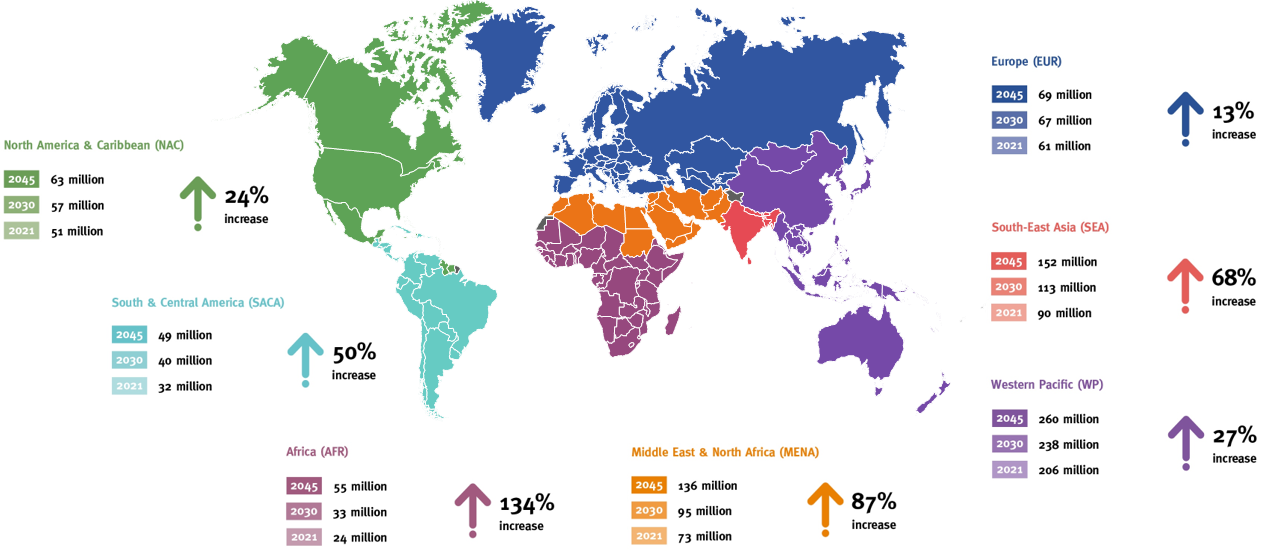
\includegraphics[width=\linewidth]{Chapter1/Fig/F1-3-01.png}
\caption[Global prevalence of diabetes]{\textbf{Global prevalence of diabetes.} Number of people with diabetes per IDF Region in 2021–2045 (20–79 years). \textit{This figure is adapted from \textbf{\cite{home_idf_nodate}}}}
\label{fig:chp1_idf}
\end{figure}
 %\st{Altogether, this makes diabetes a leading cause of mortality worldwide} 
of the foremost causes of global mortality with \textasciitilde6.7 million deaths in 2021 and inflicts a huge economic strain on healthcare systems  \textbf{\cite{home_idf_nodate}}. %These premature deaths and comorbidities %\st{due to diabetes} 
%inflict a huge economic strain on healthcare systems. The IDF estimated an expenditure of at least USD 966 billion in diabetes related causes in 2021 \textbf{\cite{home_idf_nodate}}. 
To address this burgeoning crisis and mitigate risk factors, a multifaceted approach is essential, with research efforts directed towards unraveling the complex interplay of genetic, environmental, and lifestyle factors that contribute to the development of diabetes.\\

% % ********************************** % 1.3.1  **************************************
% \subsection{Forms of Diabetes} %Section - 1.3.1 
% \label{sec:forsmDiabets}

% \colorbox{green}{text clean-up} \\

Diabetes is characterized by sustained high blood glucose concentrations (hyperglycemia) %\st{because of insufficient supply of insulin} 
resulting from inadequate insulin production, impaired insulin action, or a combination of both. Diabetes is broadly classified into two main types: \gls{t1d} and \gls{t2d}. The current classification relies both disease etiology and pathogenesis \textbf{\cite{banday_pathophysiology_2020}}, serving as a valuable tool in clinical disease assessment and therapy determination. In addition to the two major forms, there a range of other types of diabetes such as gestational diabetes (GD) which pertains to any degree of glucose intolerance or diabetes diagnosed either at the onset of pregnancy or during its course; latent autoimmune diabetes in adults (LADA) also referred as Type-1.5 diabetes, which exhibits clinical features similar to both \gls{t1d} and \gls{t2d}; neonatal diabetes (ND), a rare monogenic disorder diagnosed during the initial six months of life and maturity-onset diabetes of the young (MODY) which results from mutations in several specific genes involved in pancreatic $\beta$-cell function, and exhibits early onset. These less prevalent kinds of diabetes illustrate the broad etiological spectrum of the disease, necessitating personalized approaches to diagnosis and treatment.
% Based on this, diabetes can be divided into four main categories:\\
% \begin{enumerate}
%     \item Type 1 DM \textbf{(T1DM)}
%     \item Type 2 DM \textbf{(T2DM)} 
%     \item Gestational DM \textbf{(GDM)} and 
%     \item Diabetes associated with certain specific conditions and/or disorders.
% \end{enumerate}


%\begin{figure}[htbp]


% \subsection{Type-1 Diabetes Mellitus (T1DM)}
% \label{sec:t1dm}
% \colorbox{red}{missing references} \colorbox{green}{text clean-up} \colorbox{cyan}{might exclude from final draft} \\

% Type-1 DM (T1DM) is a chronic, autoimmune disorder in which the insulin-secreting \textbeta-cells are progressively lost, and immune cell infiltration into the pancreatic islets play a crucial role in this process. The destruction of \textbeta-cells, caused by auto-reactive CD4 and CD8 T-cells results in little to no insulin production causing hyperglycaemia. As the disease progresses, auto-antibodies targeting \textbeta-cell proteins, especially native insulin, manifest and are subsequently joined by auto-antibodies against other proteins (glutamic acid decarboxylase or zinc transporter 8), leading to an expansion of auto-reactivity and eventual development of overt clinical disease (marked by destruction of 85-90\% of \textbeta-cells).
% \newpage
% T1DM is typically \st{presents during} diagnosed in childhood and adolescence,\st{but not exclusively, and accounts for 5-10\% of all cases of diabetes} although it can occur at any age, contributing to 5-10\% of all diabetes cases \textbf{\cite{banday_pathophysiology_2020}}. The etiology of T1DM is multifactorial, involving both, genetic predisposition and environmental triggers \st{play an important role in in its the pathogenesis. of T1DM}. The current therapeutic strategy entails daily exogenous administration of insulin to maintain stable glucose levels. Alternative approaches include a hybrid-closed loop model (artificial pancreas) for regulated insulin delivery, primary islet transplantation or immuno-modulation, albeit, the latter two present their own set of challenges. Additionally, early clinical trials involving stem cell therapies, such as mesenchymal stem cell (MSC) therapy have shown promising results as potential treatments for T1DM \textbf{\cite{pathak_therapies_2019}}.

% \begin{figure}[t]
% \centering
% 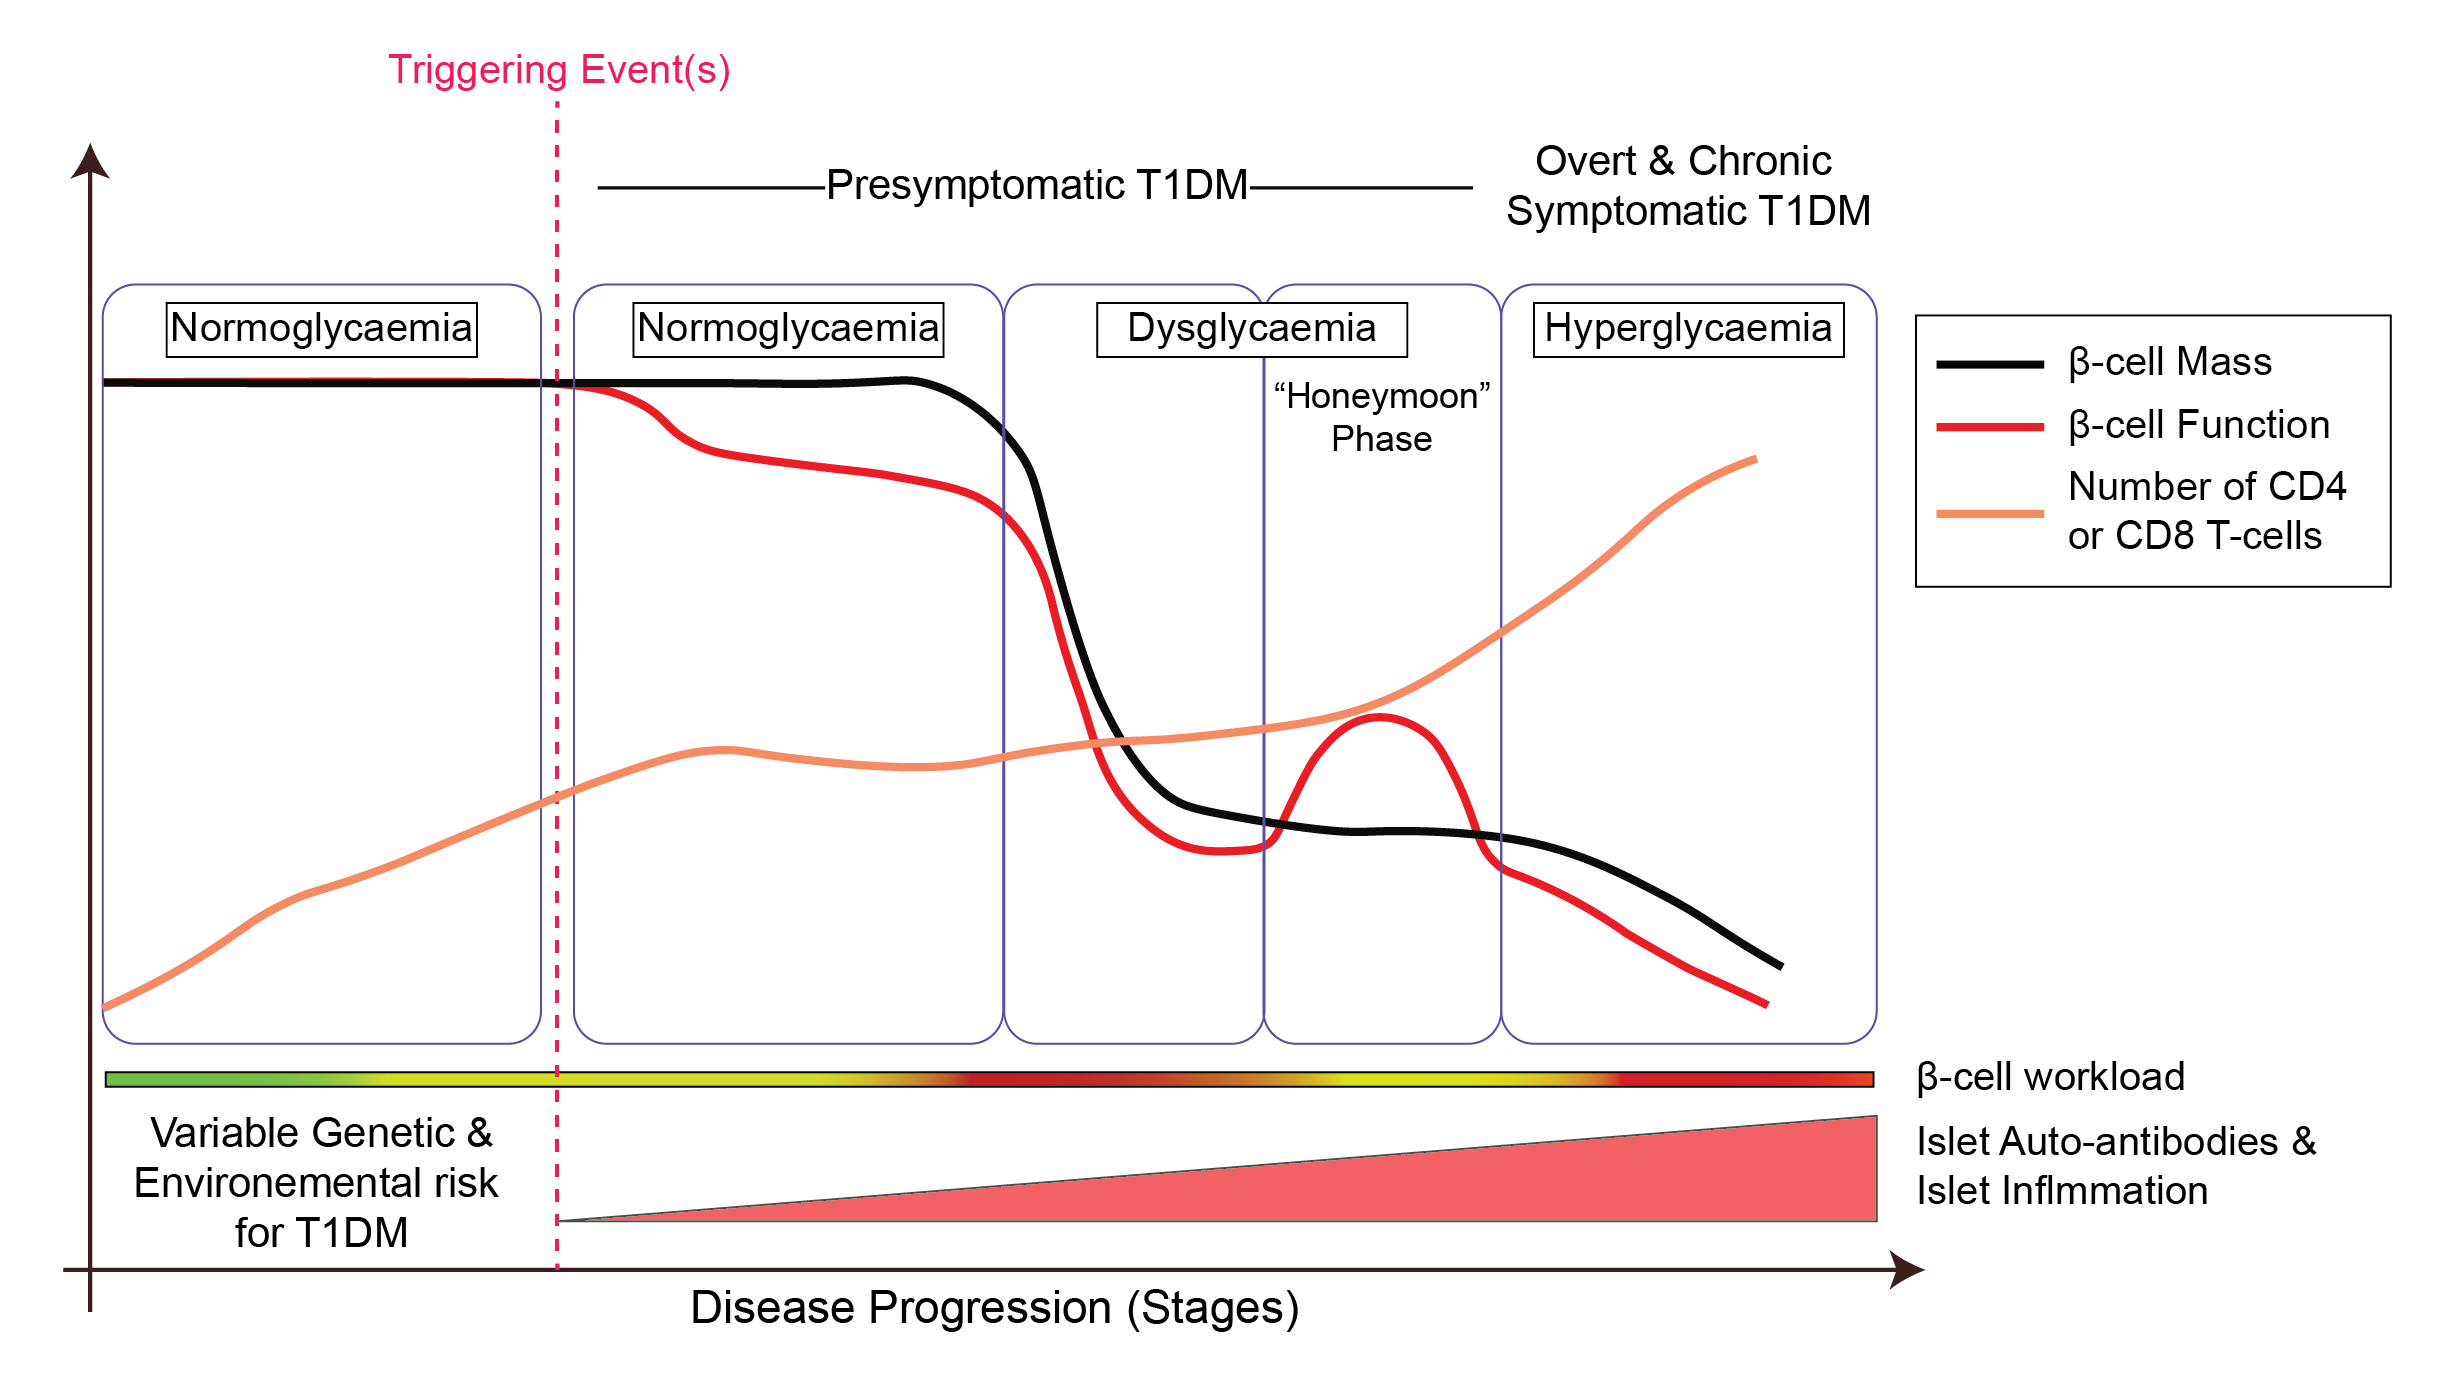
\includegraphics[width=16cm]{Chapter1/Fig/F1-3-02.png}
% \caption[diabetes]{\textbf{T1DM pathogenesis}.\\
% Adapted from several manuscripts that still need to be referenced here \textbf{\cite{chen_human_2017,von_herrath_type_2007,powers_type_2021}}}
% %\label{fig:ipsc}
% \end{figure}


\subsection{\glslink{t2d}{Type-2 Diabetes}}
\label{sec:t2dm}
%\colorbox{pink}{missing figure} \colorbox{green}{text clean-up} \\

\gls{t2d} develops from high insulin demand due to insulin resistance in peripheral target tissues. The insulin resistant state manifests several years prior to \gls{t2d} diagnosis. Functional $\beta$-cells can match the increased metabolic demand by secreting more insulin in order to maintain normal glucose levels. However, sustained demand over chronic periods leads to progressive $\beta$-cell dysfunction, resulting in glucose intolerance and overt disease \textbf{(Fig. \ref{fig:chp1_t2d_patho})}. Insulin resistance and $\beta$-cell dysfunction are considered as major hallmarks of \gls{t2d} \textbf{\cite{banday_pathophysiology_2020}}.\\

\begin{figure}[H]
    \centering
    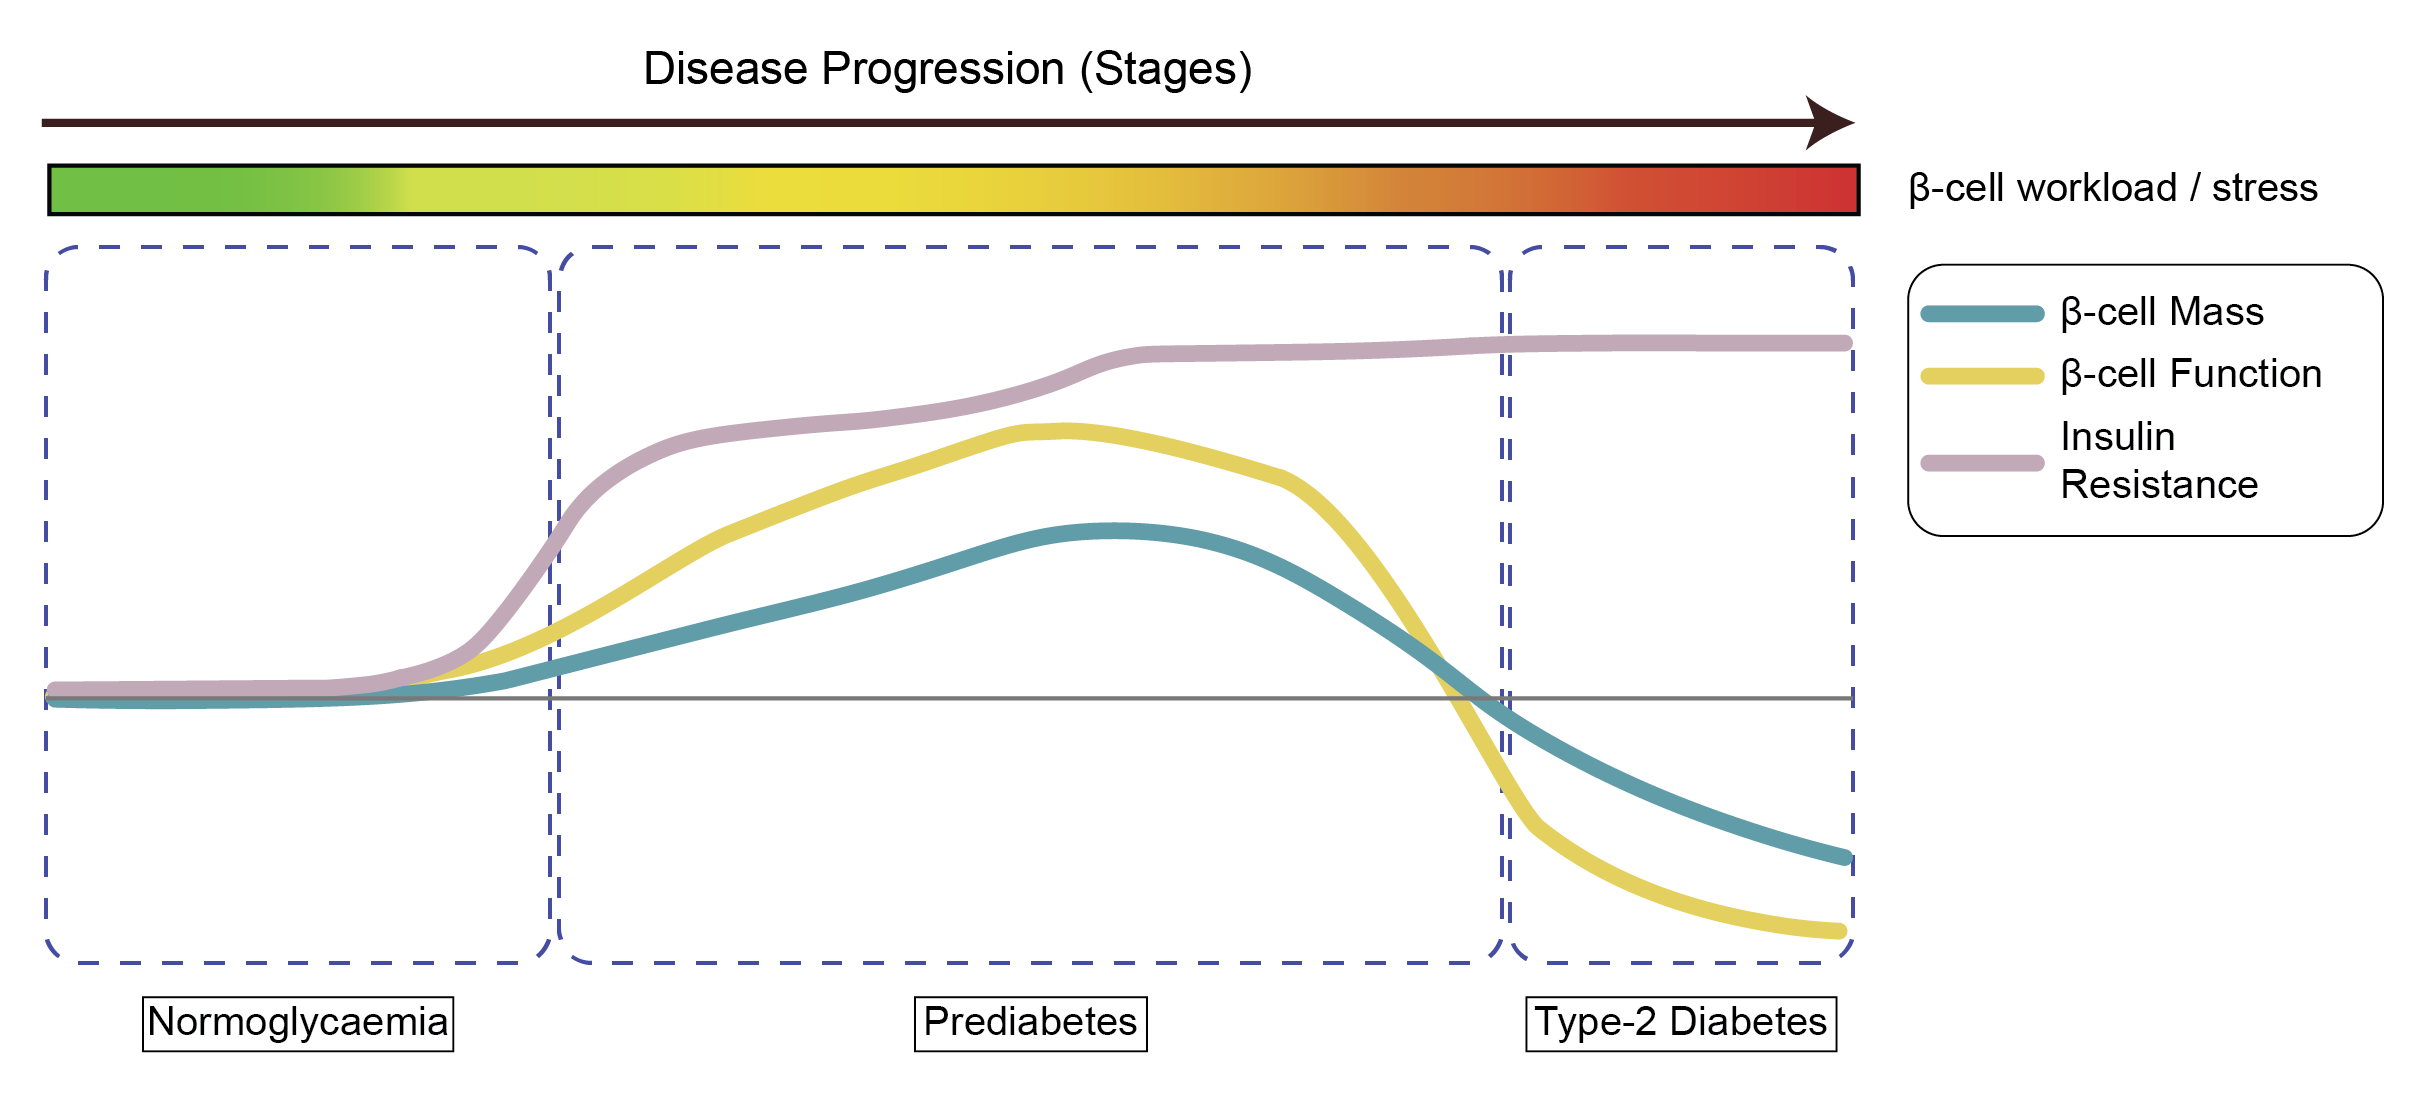
\includegraphics[width=\linewidth]{Chapter1/Fig/F1-3-04.png}
    \caption[Pathogenesis of \glslink{t2d}{T2D}]{\textbf{Insulin resistance and $\beta$-cell mass and function in the development of \gls{t2d}.} Genetic predisposition and unhealthy lifestyle lead to an increased insulin resistance, which is met by functional and morphological compensation to maintain normoglycemia, thus increasing $\beta$-cell workload. Prolonged insulin resistance leads to a prediabetic phase where chronic glucose intolerance and elevated blood glucose levels increase $\beta$-cell workload and stress, eventually causing cellular exhaustion, cell death, and the onset of hyperglycemia. Thereafter, uncontrolled hyperglycemia, leads to accelerated $\beta$-cell mass loss and functional deterioration in overt diabetes. \textit{This figure is adpated from }\textbf{\cite{chen_human_2017}}.\textit{ Reproduced with permission from Springer Nature.}}
    \label{fig:chp1_t2d_patho}
\end{figure}

While, \glslink{gwa}{GWA} studies have been able to identify the genetic susceptibility to \gls{t2d} \textbf{\cite{grarup_genetic_2014, wang_genetic_2016}}, other factors, particularly obesity have demonstrated a strong link to insulin resistance and \gls{t2d} pathogenesis. Excessive obesity causes a metabolic - overload of the adipose tissue, resulting in chronic inflammation via secretion of pro-inflammatory cytokines such as TNF-$\alpha$, IL-6, IL-1$\beta$ and MCP-1 \textbf{\cite{guilherme_adipocyte_2008}}. The macrophages recruited into the adipose tissue create a chronically inflamed state and reduce the uptake of fatty acids by skeletal muscle. The elevated levels of these free fatty acids impair signaling and insulin-stimulated glucose transport leading to the development of insulin resistance \textbf{\cite{unger_lipotoxicity_1995,uysal_protection_1997,kanda_mcp-1_2006}}. However, the critical determinant for \gls{t2d} is $\beta$-cell dysfunction \textbf{\cite{tahrani_glycaemic_2010, khin_pancreatic_2023}}, which is more severe than insulin resistance. The interplay between $\beta$-cell dysfunction and insulin resistance is highly complex; however, they likely influence each other and synergistically worsen \gls{t2d}.\\  
% Several factors are thought to contribute to $\beta$-cell dysfunction: chronic nutrient overload (glucotoxicity and glucolipotoxicity) \textbf{\cite{prentki_nutrient-induced_2020}}, insulin secretory defects \textbf{\cite{kahn_mechanisms_2006}}, reduced $\beta$-cell mass, amyloid deposition \textbf{\cite{prentki_islet_2006}} and/or islet inflammation and oxidative stresses \textbf{\cite{khin_pancreatic_2023}}.\\%\st{The role of islet inflammation in T2D and its involvement in β-cell dysfunction is discussed at length in Chapter 2.}


\par \gls{t2d} accounts for 90-95\% of all diagnosed diabetic cases \textbf{\cite{home_idf_nodate,banday_pathophysiology_2020,elsayed_2_2022}}. Due to the multi-faceted and progressive nature, the treatment for \gls{t2d} follows a step-wise approach. The very first recommended therapeutic intervention is the adoption of a healthier life style: more healthy diet, increased physical activity and maintaining a healthy body weight. The first anti-diabetic drug to be usually prescribed is Metformin, which works by reducing hepatic gluconeogenesis, delaying intestinal absorption and improving the overall insulin sensitivity \textbf{\cite{kaneto_multifaceted_2021}}, although accumulating evidence points to possible new mechanisms of actions \textbf{\cite{foretz_metformin_2023}}. The persistence of \gls{t2d} further requires additional medications, as monotherapy is insufficient to maintain normal blood glucose levels \textbf{\cite{home_idf_nodate,nathan_medical_2009}}. Other available anti-diabetic drugs include sulphonylureas, \glslink{glp1}{GLP-1} agonists, thiazolidinediones, sodium-glucose co-transporter 2 (SGLT2) inhibitors or dipeptidyl peptidase 4 (DPP-4) inhibitors \textbf{\cite{home_idf_nodate,nathan_medical_2009,american_diabetes_association_8_2017}}. Upon failure of these anti-diabetic drugs, intensive insulin therapy via exogenous administration becomes necessary in order to maintain the target range of blood glucose levels in \gls{t2d} patients and avoid health complications \textbf{\cite{home_idf_nodate}}.

% \clearpage

% \subsection{Other forms of Diabetes}
% \label{sec:otherdm}
% \colorbox{pink}{missing figure} \colorbox{cyan}{might exclude from final draft} \\\\
% T1DM and T2DM together account for most of the diabetes cases. Besides these two, there are also less common forms of diabetes:

% \subsubsection{Gestational Diabetes Mellitus (GDM)}
% Gestational diabetes mellitus (GDM) pertains to \st{is} any degree of glucose intolerance or diabetes diagnosed either at the onset of pregnancy or during its course \st{pregnancy}, usually in second or third trimester. Unlike preexisting diabetes in women, GDM usually resolves \st{soon after childbirth} shortly after childbirth or upon termination of pregnancy. \st{and is different from any preexisting diabetes in women.} Blood glucose levels undergo elevation during the third trimester, and when they reach diabetic levels, the condition is described as GDM. The risk of GDM increases with age, obesity, previous pregnancies and any previous history of glucose intolerance or GDM itself. Additionally, GDM has been associated with an increase lifetime risk of developing T2DM. Therefore, individuals need to be assessed for persistent diabetes postpartum, in order to ensure early diagnosis \textbf{\cite{banday_pathophysiology_2020,egan_what_2019}}.

% \subsubsection{Latent Autoimmune Diabetes in Adults (LADA)}
% Latent autoimmune diabetes in adults (LADA), also referred as Type-1.5 diabetes, exhibits clinical features similar to both T1DM and T2DM. It is the most common form of adult-onset autoimmune diabetes, accounting for 2-12\% of all diabetic cases. LADA is characterized by the presence of certain autoantibodies and its strong association with the human leukocyte antigen (HLA) region that are associated with immune response, including autoimmunity. Patients with LADA often exhibit insulin resistance similar to T2D. However, LADA is genetically distinct from both T1DM and T2DM despite sharing genetic risk factors \textbf{\cite{banday_pathophysiology_2020,carlsson_etiology_2019,andersen_latent_2010,andersen_type_2014,cervin_genetic_2008}}. 

% \subsubsection{Monogenic Diabetes}
% Monogenic diabetes arise \st{from defects in single gene}due to single-gene defects in contrast to the multifactorial etiologies of T1DM or T2DM\st{, which involved contributions of multiple genes and environmental factors}. Monogenic diabetes are less common contributing to 1.5 – 2\% of total diabetes cases, and are often misdiagnosed as either T1DM or T2DM. In recent years, with several genome-wide association studies, an increasing number of monogenic diabetes are being discovered\st{. Therefore, the true prevalence of this type may be underestimated.}, suggesting that its true prevalence might be underestimated. The spectrum of  monogenic diabetes encompasses conditions such as \st{forms present a broad spectrum from }maturity-onset diabetes of the young (MODY), neonatal diabetes mellitus (NDM) and rare diabetes-associated syndromic diseases \textbf{\cite{home_idf_nodate}}. 

% \subsubsection{Maturity-onset diabetes of the young (MODY)}
% Maturity-onset diabetes of the young (MODY)\st{, also known as monogenic diabetes,} results from mutations in several specific genes involved in pancreatic β-cell function thereby affecting glucose sensing and subsequent insulin secretion, with minimal to no defects in insulin action. As the name suggests, MODY demonstrates an early onset, with glucose intolerance and hyperglycemia manifesting usually before the age of 25, although it can occur late in life. It is distinct from both T1DM and T2DM and follows an autosomal dominant inheritance pattern. At least 14 genes associated with MODY have been identified so far and these are mostly located on different chromosomes. The most prevalent forms of MODY are designated as MODY2 (glucokinase gene, \textit{GCK}), MODY3 (transcription factor, \textit{HNF1A}) and MODY1 (transcription factor \textit{HNF4A}), together accounting for more than 80\% of MODY cases \textbf{\cite{banday_pathophysiology_2020,american_diabetes_association_2_2020}}.

% \subsubsection{Neonatal Diabetes Mellitus (NDM)}
% Neonatal diabetes mellitus (NDM) is a monogenic diabetes diagnosed during the \st{first 6} initial six months of life. The genetic abnormalities associated with NDM result in β-cell dysfunction and decreased β-cell mass due to increased apoptotic or non-apoptotic cell death leading to severe hyperglycemia along with hypoinsulinemia \textbf{\cite{banday_pathophysiology_2020}}. NDM is a rare disorder (incidence rate - 1 per 500,000 – 300,000 live births) \textbf{\cite{banday_pathophysiology_2020,iafusco_minimal_2012,polak_neonatal_2007}}  and is highly distinct from T1DM in both its origin and nature of inborn pancreatic disorder. The genetic defects also result in developmental \st{abnormalities}irregularities of pancreas and/or its islets and in extremely rare \st{cases} instances, their complete absence, leading to decreased insulin production and secretion, and in the latter case, an absolute deficiency, thereby requiring insulin replacement therapy. Based on the clinical presentation, NDM can be either transient (most common form – resulting from overexpression of genes on chromosome region \textit{6q24}) or permanent (less common form – resulting from heterozygous autosomal dominant mutations in the genes encoding for subunits of β-cell K\textsubscript{ATP channel}).%\clearpage
% \\\\Furthermore, various other forms of diabetes arise from diverse contributing factors, which are elucidated in this comprehensive review \textbf{\cite{banday_pathophysiology_2020}}.
% \\\\
% In summary, DM is a complex and heterogeneous metabolic disorder characterized by persistent hyperglycaemia and loss of functional β-cell mass. The pathogenesis of DM involves several factors, including genetics and strong environmental influences. While there are effective and personalized treatments available for DM, these strategies do not halt the progression of the disorder. Therefore, management of DM involves lifelong medication and continuous care to maintain health and prevent secondary complications. 


%The overall aim of this thesis is to provide suitable computational methods for the identification of cell type and context-specific eQTL using single cell expression profiles, and explore their application across a range of human iPSC-derived cell types, using data from the \gls{hipsci} project.\\

%Specifically, in \textbf{Chapter \ref{chapter2}}, I provide an overview of the use of linear and \glspl{lmm} for genetic association analyses, focusing on their application in \gls{eqtl} mapping.\\

%In \textbf{Chapter \ref{chapter3}}, I describe best-practice approaches to perform \gls{eqtl} mapping using \gls{scrnaseq} profiles and demonstrate these methods on matched bulk and single cell expression of around 100 human \gls{ipsc} lines. \\

%In \textbf{Chapter \ref{chapter4}}, I present a dataset of almost 40,000 cells from 125 human \gls{ipsc} lines differentiating to definitive endoderm, and demonstrate different approaches to \gls{eqtl} mapping using \gls{scrnaseq} data, identifying genetic variants that affect gene expression dynamically along differentiation and across other cellular states. \\

%In \textbf{Chapter \ref{chapter5}}, I present a dataset of over one million cells from 215 human \gls{ipsc} lines differentiating to midbrain dopaminergic neurons. We identify thousands of \glspl{eqtl} across a number of cell types and upon external stimulation. In addition, we identify hundreds of colocalisation events with variants that are known to be associated with neurological traits and diseases. Moreover, we investigate sources of variation in the capacity of individual cell lines to differentiate toward neurons.\\

%Finally, in \textbf{Chapter \ref{chapter6}}, I conclude and discuss future directions.

%\newpage

% ***************************************************************

% %********************************** %Second Section  **************************************
\section{Endocrine Pancreas: Morphology and Physiology}  %Section - 1.2
\label{sec:endopanc}

%\colorbox{pink}{incomplete figure} \colorbox{green}{text clean-up}\\

The pancreas is a glandular organ originating from the endoderm and located in the abdomen, behind the stomach \textbf{\cite{shih_pancreas_2013}}. It plays a %\st{vital organ originating from the endoderm} 
critical role 
%\st{with a central role} 
in energy homeostasis
%\st{. The pancreas exerts its effects} 
by secreting digestive enzymes and releasing metabolic hormones \textbf{\cite{kimmel_molecular_2010, baron_single-cell_2016}}. %The pancreas is the only organ with \st{functions both, as an} exocrine and endocrine \st{gland} functions.  \st{The exocrine} 
Majority of the pancreatic mass (\textasciitilde 90\%) is comprised of the exocrine tissue, consisting of acinar, 
%centro-acinar 
and ductal cells \textbf{\cite{pandiri_overview_2014}}. The acinar cells secrete digestive enzymes, which catalyze the breakdown of proteins (peptidases), carbohydrates (amylases), and lipids (lipases). The ductal system transports these digestive enzymes to the duodenum and gastrointestinal tract \textbf{\cite{shih_pancreas_2013, baron_single-cell_2016}}.  In addition to this, the 
%\st{ductal system} 
pancreatic ducts %along with the centro-acinar cells, 
secrete large volumes of bicarbonate-rich fluid, resulting in the flushing of acinar secretions \textbf{\cite{pandiri_overview_2014, low_pancreatic_2010}}. The endocrine component, called islets of Langerhans (short islets), comprise 1-2\%, and the interstitium with vasculature, lymphatics, nerves, and fibrous connective stroma make up the remainder of the tissue mass \textbf{\cite{pandiri_overview_2014}}. %The islets are named after Paul Langerhans, who in 1869, through exhaustive histological studies discovered that the pancreas was a heterogeneous organ comprised of different structures. 
The islets, embedded within the exocrine tissue and scattered throughout the whole pancreas, consist of several unique cell types, all of which secrete different hormones and peptides for regulating %\st{glucose homeostasis} 
blood glucose level \textbf{\cite{shih_pancreas_2013, baron_single-cell_2016}} and influencing exocrine function. The alpha \textbf{($\alpha$)} cells release glucagon, the beta \textbf{($\beta$)} cells produce insulin and amylin, the gamma \textbf{($\gamma$)} or PP-cells produce pancreatic polypeptide, the delta \textbf{($\delta$)} cells produce somatostatin and the epsilon \textbf{($\epsilon$)} cells produce ghrelin \textbf{\cite{mastracci_endocrine_2012} (Fig.\ref{fig1-1})}.\\

\begin{figure}[t]
\centering
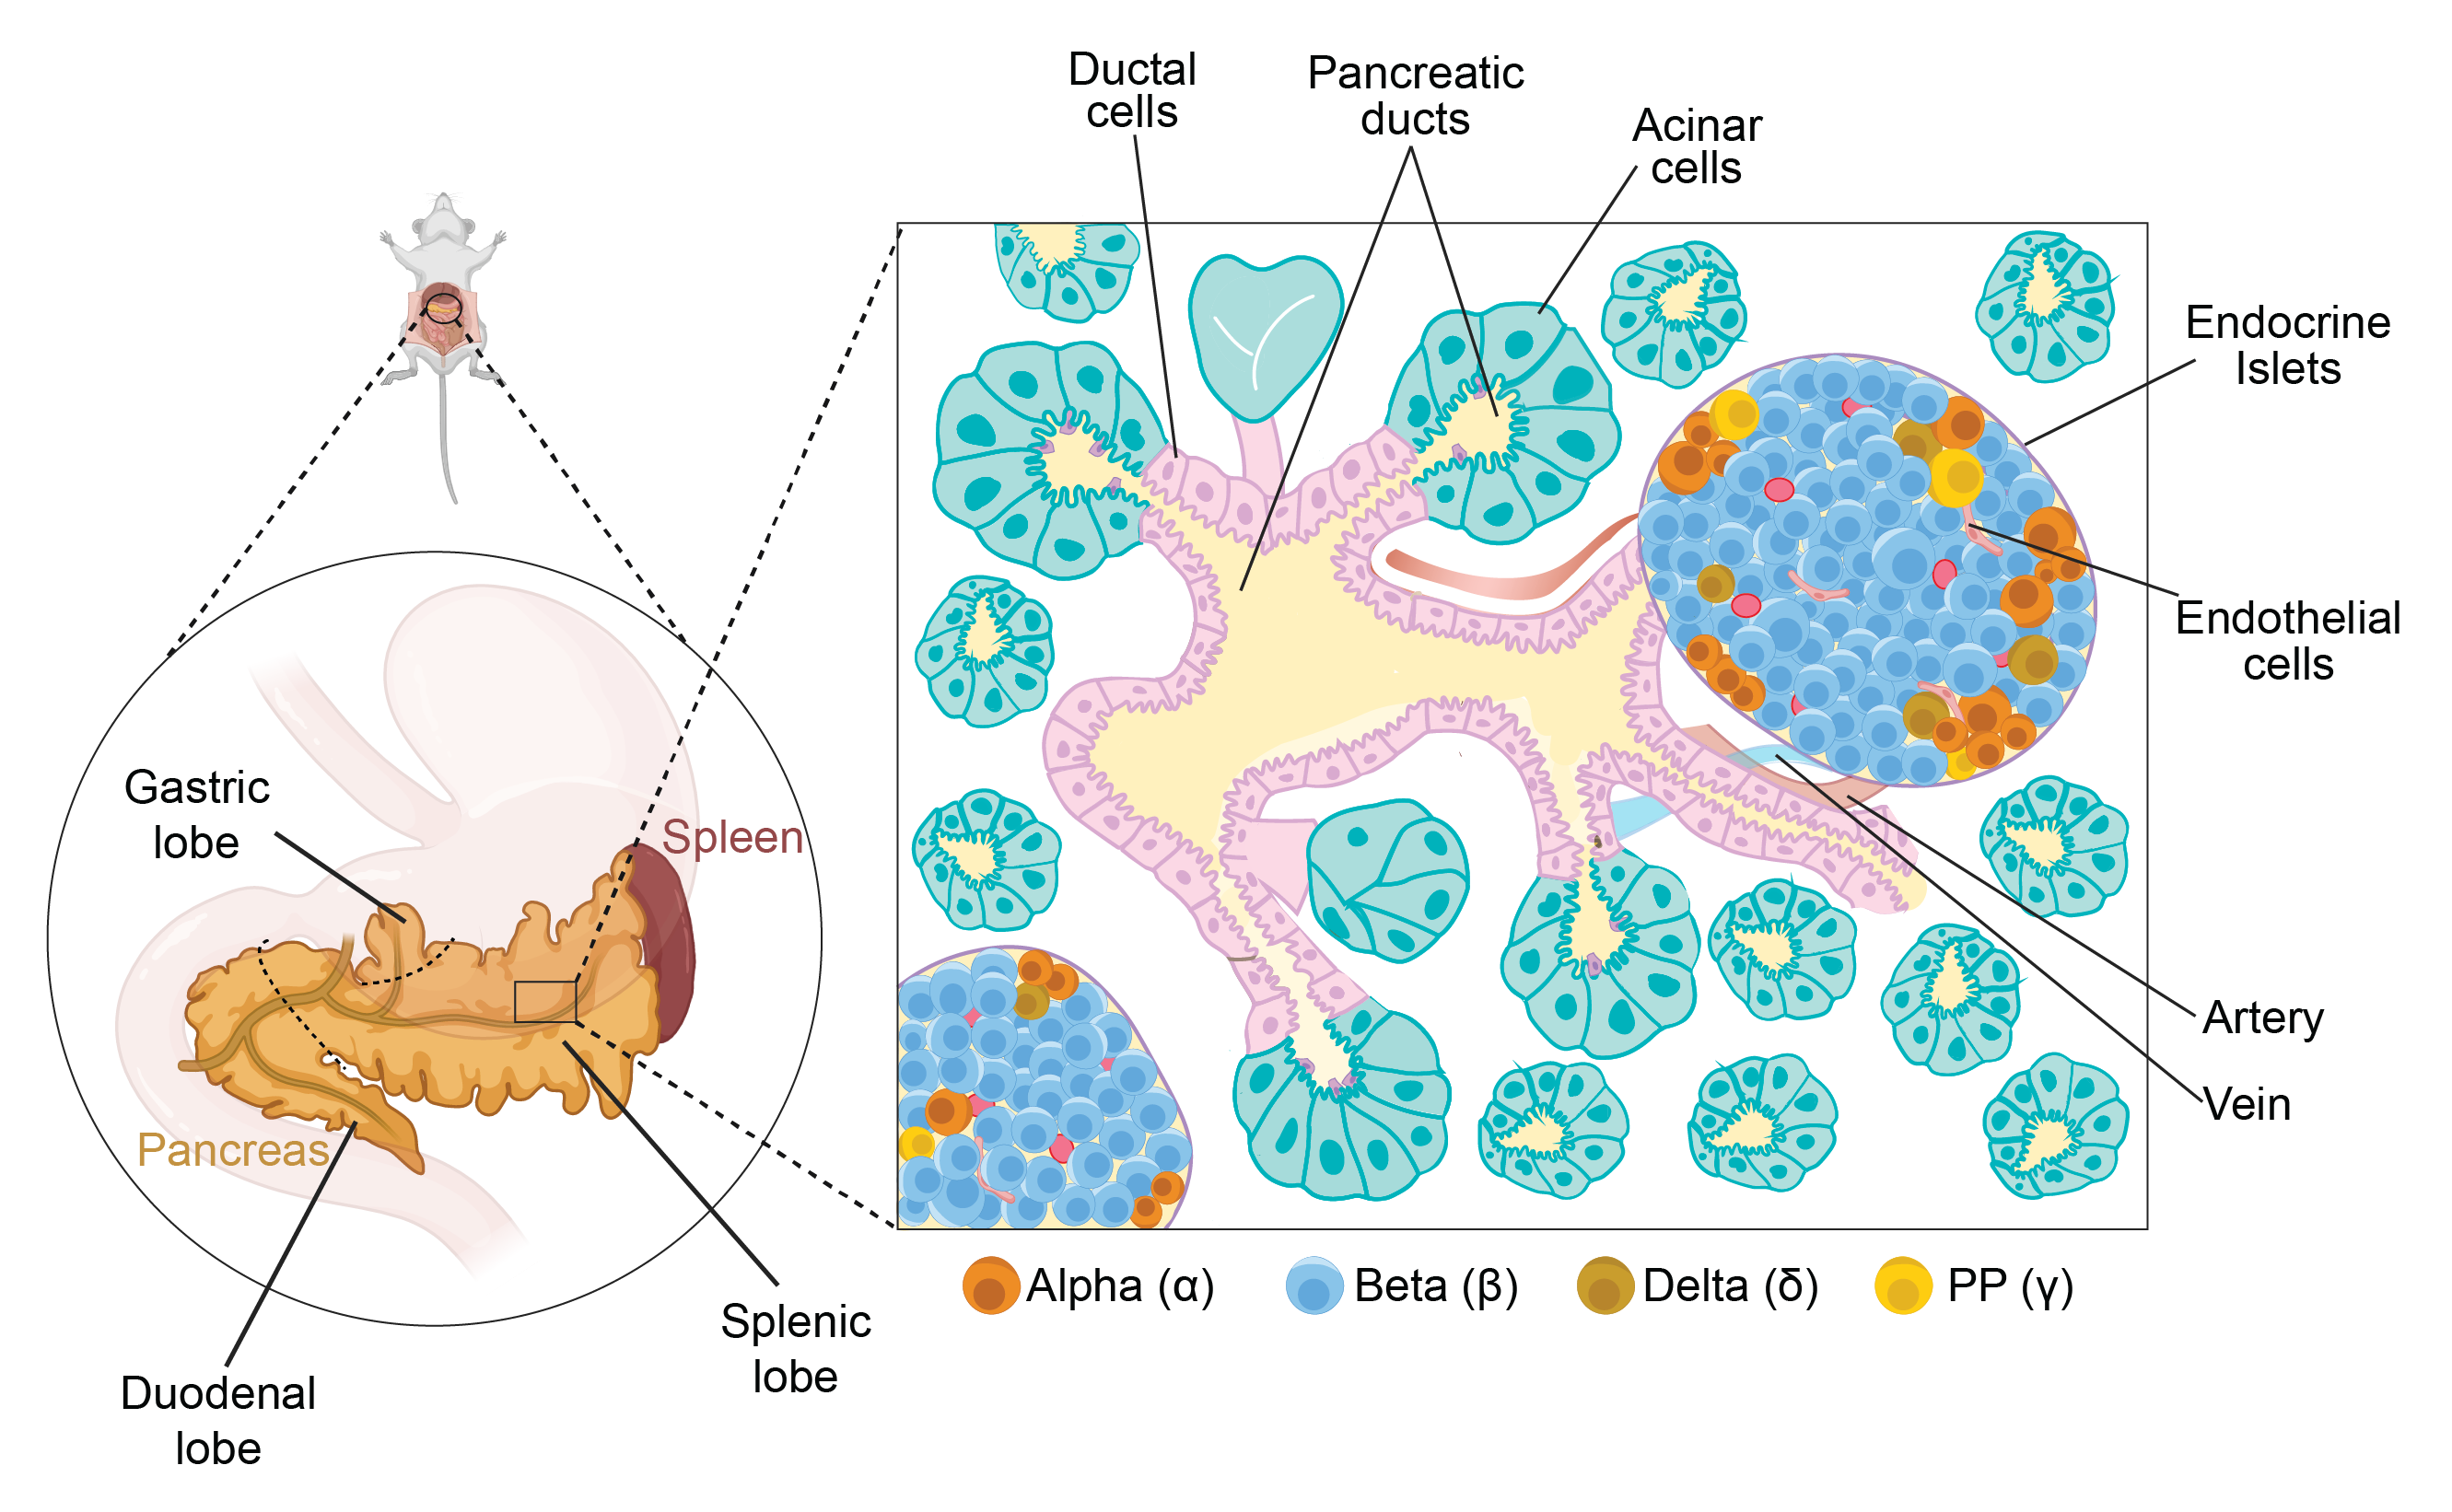
\includegraphics[width=\linewidth]{Chapter1/Fig/F1-1-01.png}
\caption[Morphology of mouse pancreatic tissue]{\textbf{Overview of the anatomy of pancreas in adult mice.} The pancreas is divided into three lobes: duodenal, gastric and splenic. The pancreatic tissue consists of exocrine cells such as acinar and ductal cells and the endocrine pancreas consists of small cell clusters called islets. The islets contain endocrine cell-types, namely $\alpha$-cells, $\beta$-cells, $\delta$-cells, and PP-cells. The islets are surrounded by a dense capillary network through which the hormones are released. \textit{This figure is adapted from }\textbf{\cite{shih_pancreas_2013,jain_targeting_2022}}.\textit{ Reproduced with permission from Springer Nature.}}
\label{fig1-1}
\end{figure}


% %\begin{figure}[htbp]
% \begin{figure}[H]
% \centering
% 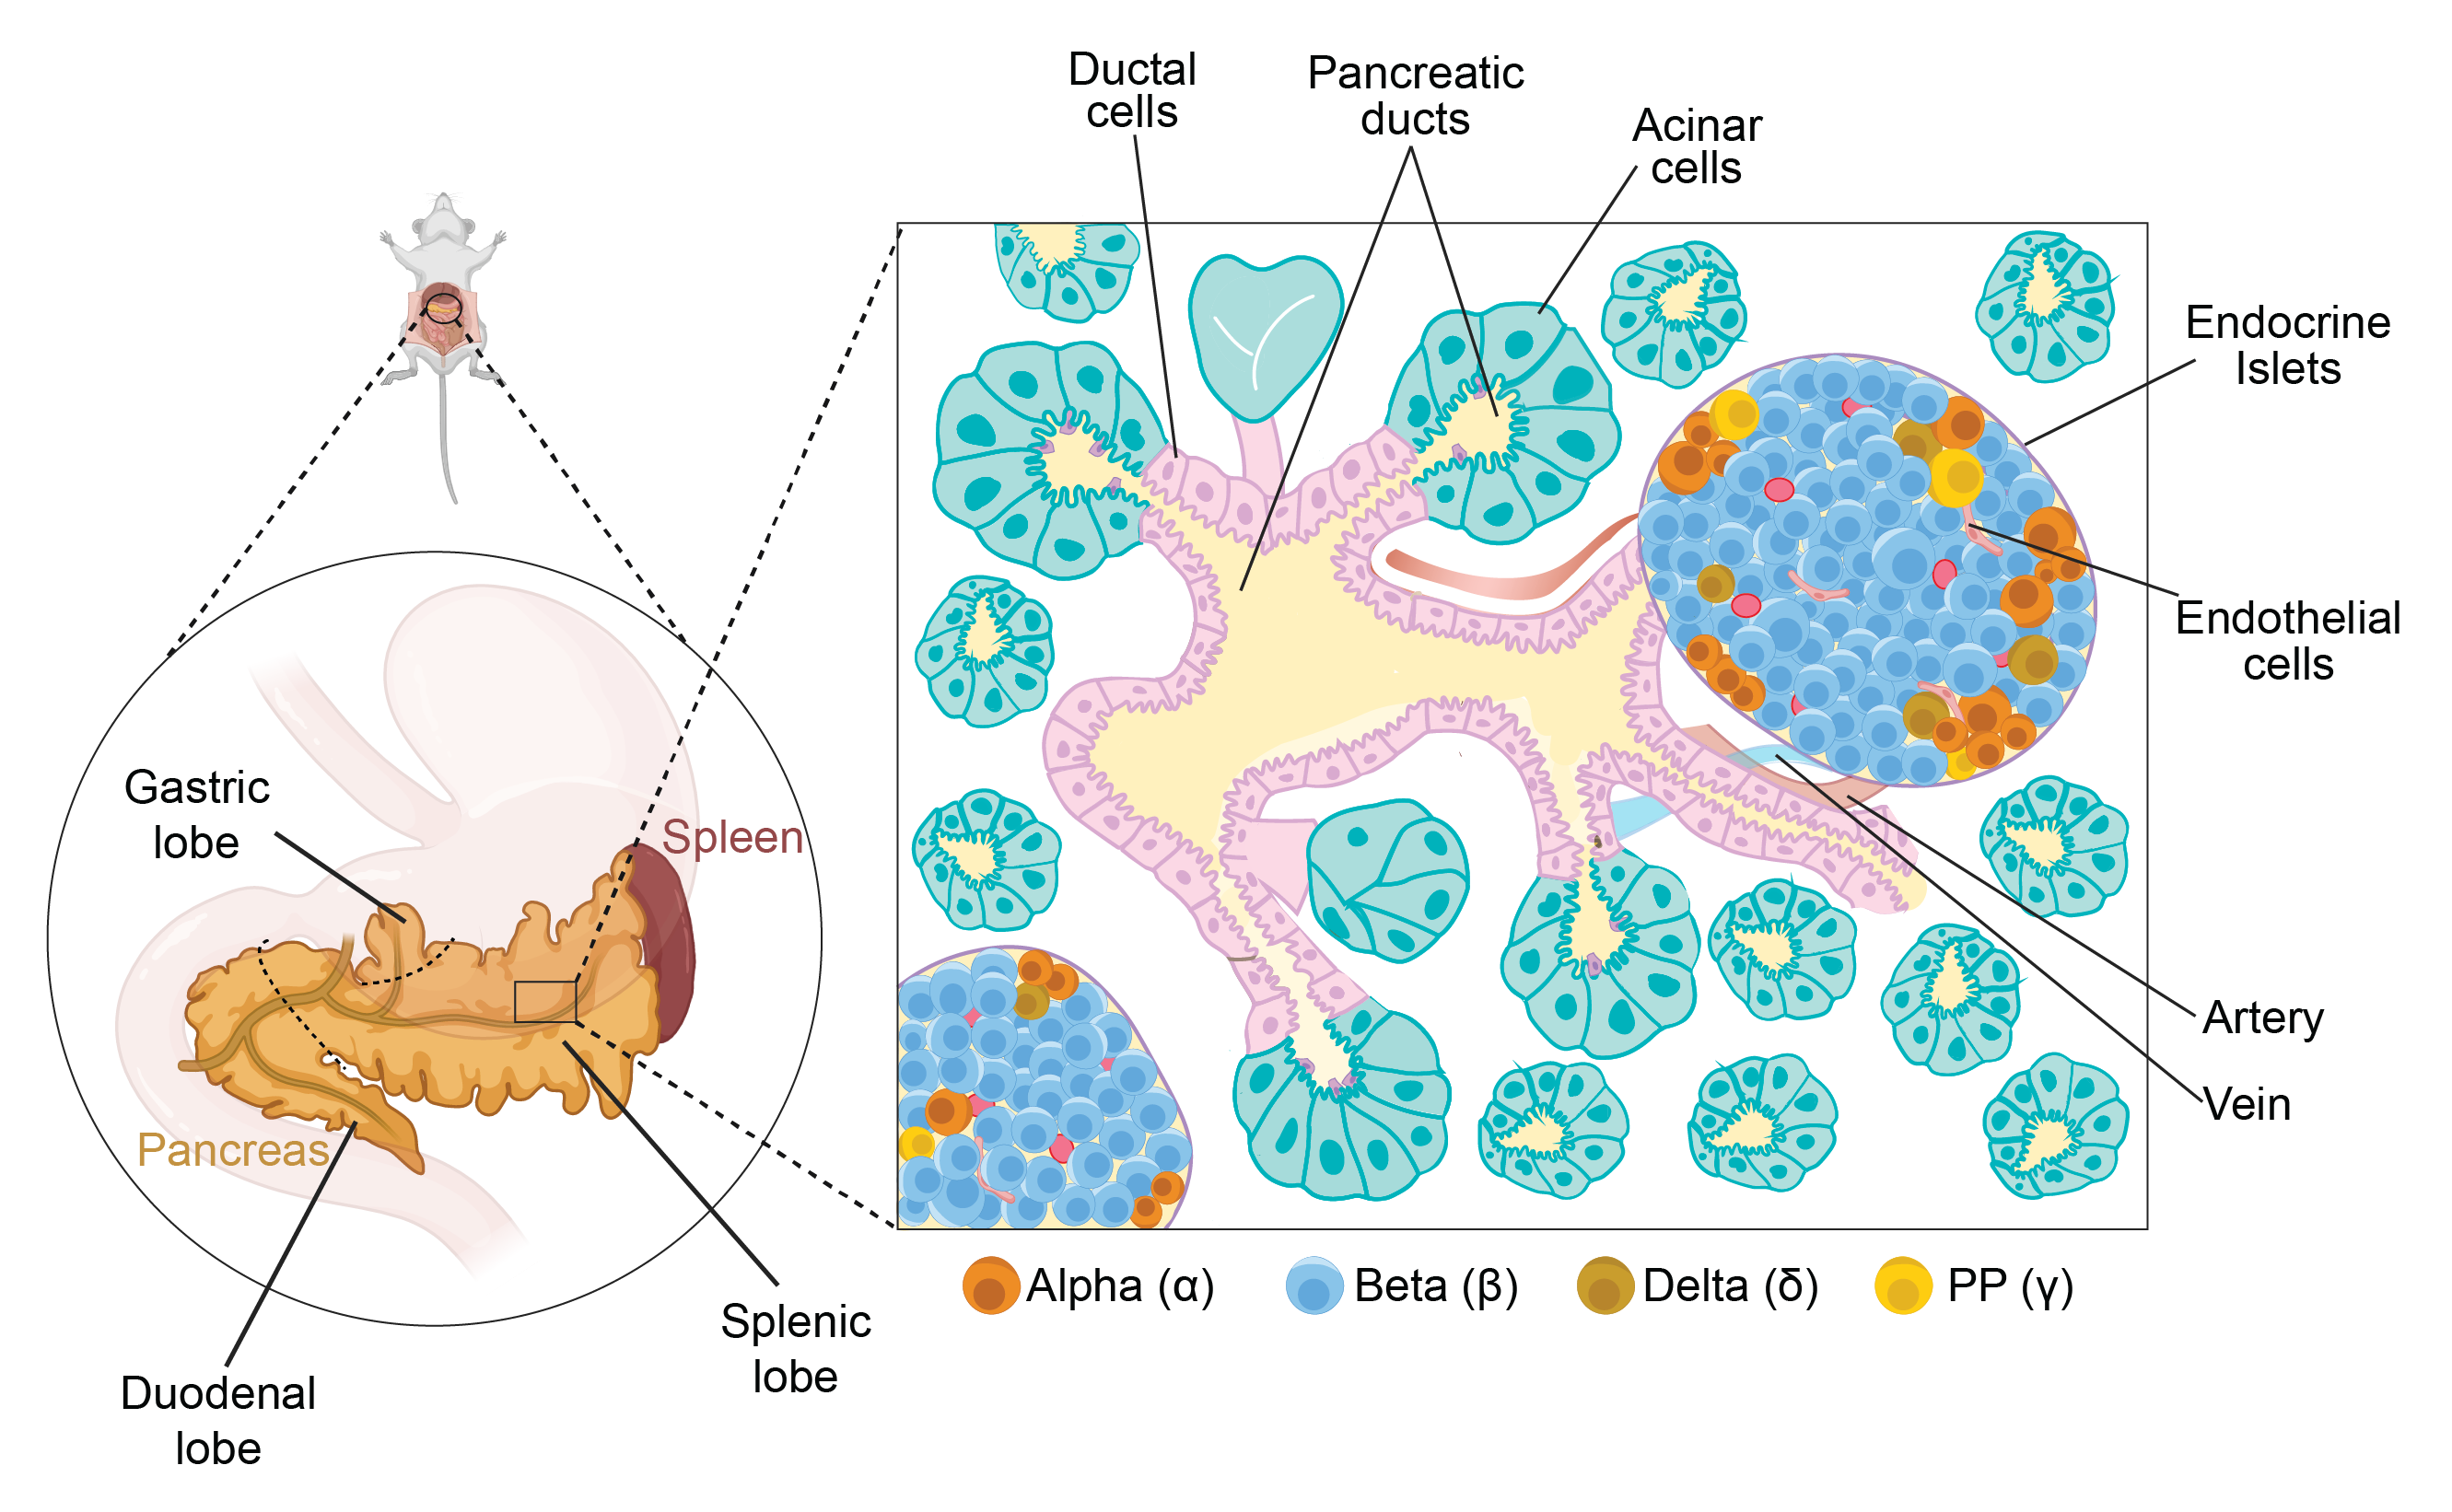
\includegraphics[width=\linewidth]{Chapter1/Fig/F1-1-01.png}
% \caption[sec1-1endopanc]{\textbf{Endocrine Pancreas}}
% \label{fig1-1}
% \end{figure}

\par In rodents such as mice, the islets consist of \textasciitilde75–80\% $\beta$-cells, forming a rich core and \textasciitilde15–20\% $\alpha$-cells and the rest is made up by the remaining endocrine cells ($\delta$-cells and PP-cells, <10\% and $\epsilon$-cells, <1\%), forming the mantle of the islet. In contrast, endocrine cells in the human islets seem to be randomly distributed, and have proportionally fewer $\beta$-cells (\textasciitilde55-75\%) and more $\alpha$-cells (\textasciitilde30-45\%), likely suggesting the major role of glucagon hormone secretion in humans. The variability in cell distribution results in more heterotypic contacts between the endocrine cells in human islets \textbf{\cite{walker_human_2021}}. %It has been shown in both mice and humans, that the islet architecture is size-dependent, with smaller islets displaying the core-mantle structure and larger islets with more complex organization \textbf{\cite{dolensek_structural_2015}}.
Additional differences in the innervation patterns and presence of smooth muscle cells throughout the vascular network also exist between mouse and human islets \textbf{\cite{rodriguez-diaz_autonomic_2011}}. %\st{It is likely that these islet architecture differences between mouse and human}
These islet architecture differences between mouse and human likely contribute to physiological differences regarding islet function \textbf{\cite{cabrera_unique_2006}}. %The pancreatic tissue in mice is a diffused lobular organ consisting of the duodenal, the splenic, and the gastric lobes. In humans, the pancreas exhibits \st{is} a more compact and well-defined structure, comprising of \st{into three major parts:} the head, the body, and the tail.
%The pancreas receives a rich vascular supply and the macro-vascular network is conserved in humans and rodents \textbf{\cite{muratore_vascular_2021}}.
Although the islets comprise 1-2\% of the pancreas, they receive up to 20\% of the pancreatic blood supply \textbf{\cite{muratore_vascular_2021,jansson_glucose-induced_1986}}. 
%\st{The dense vascularization}
This remarkable vascularity of islets is necessary for normal islet function and likely explains how fluctuations in blood glucose are %\st{sensed} 
detected, %\st{and lead}
leading to rapid and %\st{large}
substantial changes in the secretion of pancreatic hormones \textbf{(Fig. \ref{fig:chp1_mouse_human_islets})}.\\

\begin{figure}[H]
    \centering
    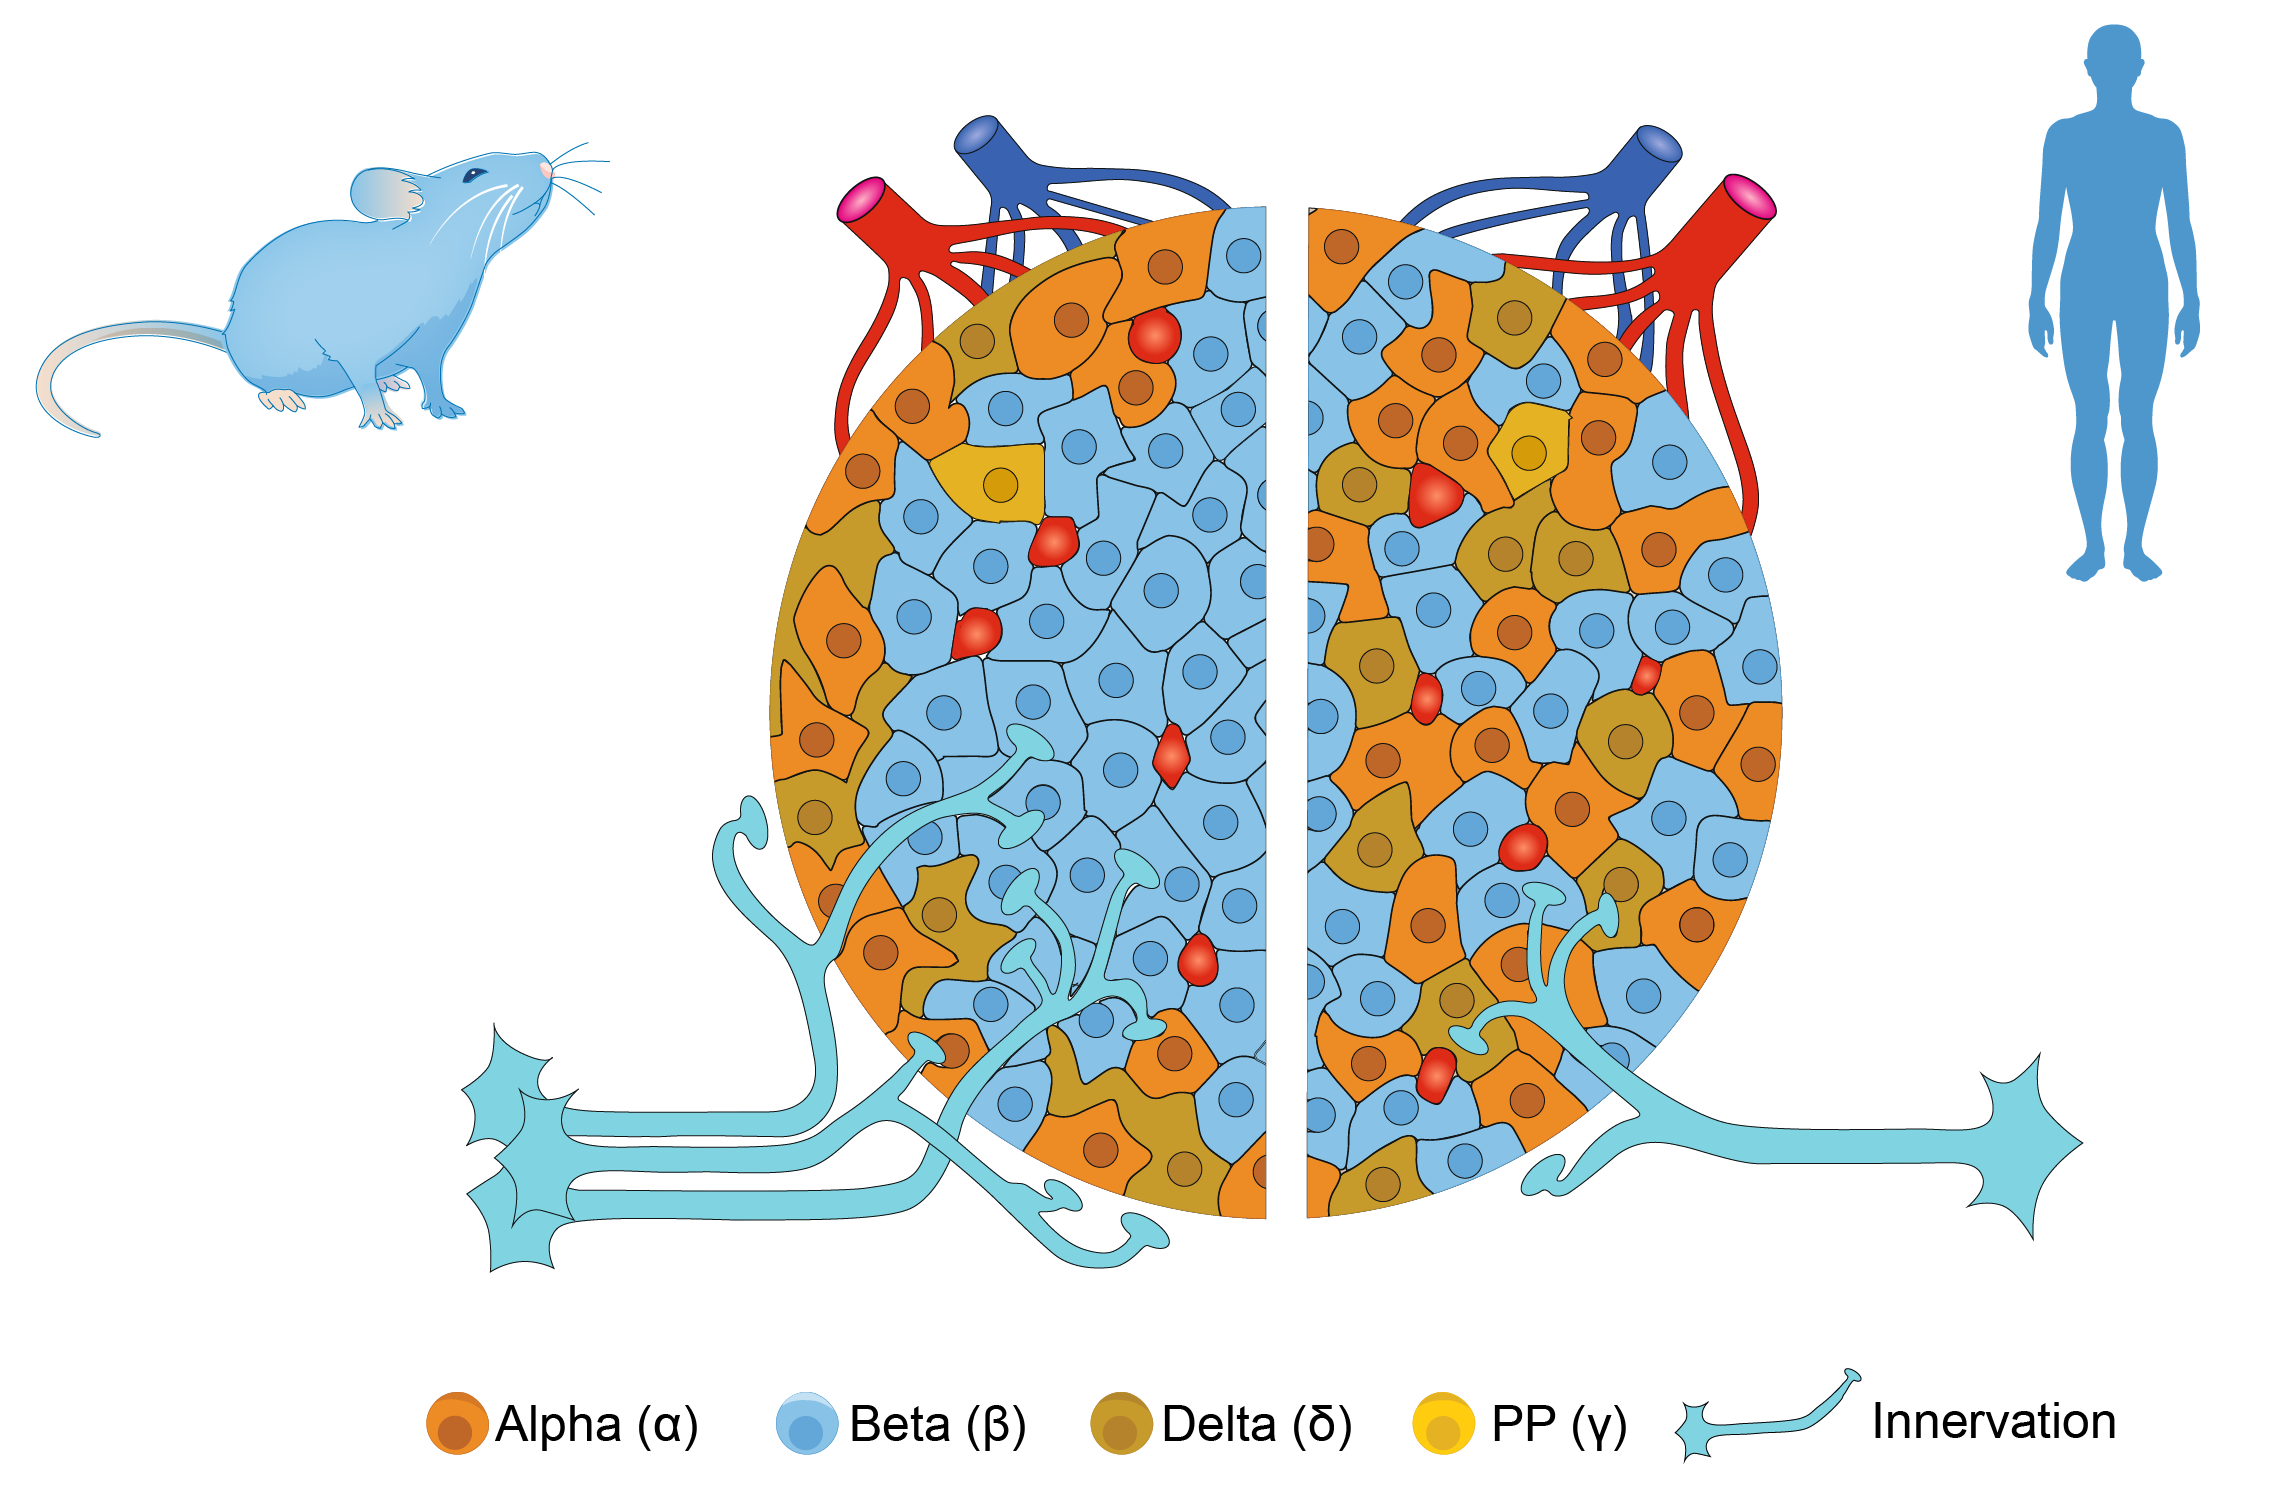
\includegraphics[width=12cm]{Chapter1/Fig/F1-2-1-01.png}
    \caption[Comparative architecture of mouse and human pancreatic islets]{\textbf{Comparative architecture of mouse and human pancreatic islets.} Islet architecture from a healthy adult mouse and a healthy adult human pancreas displaying the various endocrine cell-types. The mouse islets depict a core and mantle structure with centrally located $\beta$-cells, whereas the human islets depict a more random distribution with fewer $\beta$-cells. Additionally, the vascularization and innervation of the islets are depicted. The mouse islets are more densely innervated than those in humans. \textit{This figure is adapted from }\textbf{\cite{jain_targeting_2022,noguchi_integrating_2019}}. \textit{ Reproduced with permission from Springer Nature.}}
    \label{fig:chp1_mouse_human_islets}
\end{figure}

\par To summarize, the pancreatic islets are regarded as a coordinated mini-organ that serves as a remarkable regulator, integrating systemic and local cues to fine-tune blood glucose levels by the synthesis and appropriate secretion of several metabolic hormones by the diverse cell types in the islet microenvironment.


\clearpage


% ***************************************************************

%************************ %Third Section %****************************************************************
\section{ Islet $\beta$-cells}  %Section - 1.3
\label{sec:islet-betacells}  

% ********************************** % 1.3.1  **************************************
\subsection{Endocrine cell Development} %Section - 1.3.1 
\label{sec:endocelldev}

%\colorbox{pink}{missing figure} \colorbox{green}{text clean-up}\\

% Pancreas organogenesis is a \st{highly} conserved process during fetal development and comprises a tightly coordinated and regulated interplay of complex signaling events. During this step-wise program, the pancreas develops from a simple bud-like structure to a \st{final} mature, highly branched organ containing several specialized cell types. In mice, the pancreas specification begins at embryonic day 8.5 \textbf{(e8.5)} with the formation of dorsal and ventral pre-pancreatic regions in the foregut endoderm \textbf{\cite{shih_pancreas_2013, slack_developmental_1995}}. The pancreas development becomes morphologically evident at  \textbf{\textasciitilde e9.5} when the presumptive pancreatic regions in the endoderm undergo thickening and eventually result in the emergence of pancreatic buds \textbf{\cite{shih_pancreas_2013}}. Over the next 2-3 days, the pancreatic buds continue to elongate, accompanied by the stratification of the epithelium and the formation of multiple micro-lumens \textbf{\cite{pan_pancreas_2011}}. At \textbf{\textasciitilde e12.5}, as a result of both due to gut rotation and elongation of the dorsal and ventral stalks, the pancreatic buds (dorsal and ventral) come into contact and fuse into a single organ. This early phase of pancreatic development is referred to as the \textbf{`primary transition'}.\\

Pancreas organogenesis is a conserved process during fetal development and occurs in two phases. The early phase of pancreatic organ development is referred to as the \textbf{primary transition}. The vast majority of the endocrine cells arise from the endocrine progenitors during the \textbf{secondary transition} phase \textbf{\cite{pan_pancreas_2011}}. %However, glucagon-containing α-cells can be seen as early as \textbf{e9} in the primordium \textbf{\cite{pictet_ultrastructural_1972,gittes_developmental_2009}}. 
The fate decision during the secondary transition is determined by graded \textit{Notch} activity. Lower \textit{Notch} activity leads to \textit{Sox9} expression, which is an activator of \textit{Ngn3} \textbf{\cite{shih_pancreas_2013}}, a basic-helix-loop-helix (bHLH) \gls{tf} and master regulator of endocrinogenesis \textbf{\cite{gu_direct_2002}}. Cells that do not escape \textit{Notch} signaling express both \textit{Hes1} and \textit{Sox9}, resulting in \textit{Ngn3} repression and eventual contribution to the ductal tree. %\st{However, no signals have yet been identified that could account such a segregated expression pattern of Ngn3.} 
After \textit{Ngn3} expression, endocrine progenitors exit the cell-cycle and delaminate into surrounding stromal tissue \textbf{\cite{shih_pancreas_2013, gouzi_neurogenin3_2011, miyatsuka_neurogenin3_2011}}. These \textit{Ngn3\textsuperscript{+}} cells are uni-potent and as a whole can generate the five different endocrine cell types \textbf{\cite{shih_pancreas_2013,gu_direct_2002,miyatsuka_neurogenin3_2011}}. The timing and strength of \textit{Ngn3} expression determines the efficiency of endocrine cell formation and the cell type: early \textit{Ngn3} expression results in formation of $\alpha$-cells while delayed expression of \textit{Ngn3}  generates $\beta$- and $\delta$-cells followed by PP-cells \textbf{\cite{johansson_temporal_2007}}.

%\clearpage


% ********************************** % 1.3.2  **************************************
\subsection{$\beta$-cell maturation} %Section - 1.3.2
\label{sec:betamat}
%\colorbox{pink}{missing figure} \colorbox{green}{text clean-up} \colorbox{red}{missing references}\\

Critical \glspl{tf} such as \textit{Pax4}, \textit{Pdx1} and \textit{Nkx6-1} control the determination of β-cell fate. %On the contrary, \textit{Arx} determines α-cell identity. Both \textit{Pax4} and \textit{Arx} are targets of \textit{Ngn3} and are co-expressed, after which they begin to repress each other. 
 After birth, immature $\beta$-cells undergo step-wise maturation to become fully mature cells. $\beta$-cell maturation is continuation of $\beta$-cell development and occurs post-natally in mammals \textbf{\cite{barsby_maturation_2022}}. Most of the current understanding of $\beta$-cell maturation process is derived from neonatal rodent islets, as similar data from humans is difficult to collect \textbf{\cite{liu_all_2017, salinno_-cell_2019}}. After birth, immature $\beta$-cells undergo several steps to become fully mature and functional cells characterized by tightly controlled insulin secretion in response to glucose. The immature $\beta$-cells are organized into clusters, forming proto-islets \textbf{\cite{salinno_-cell_2019}}, which eventually undergo structural rearrangements to form the compacted core and mantle architecture \textbf{\cite{}}. The developmentally immature $\beta$-cells are characterized by a strong proliferative capacity, thereby resulting in a general increase in $\beta$-cell mass. The immature $\beta$-cells present insulin granules but display leaky insulin secretion wherein they have a decreased glucose threshold for stimulated insulin secretion \textbf{\cite{liu_all_2017, blum_functional_2012}} and are less glucose-responsive thereby affecting their ability to regulate insulin secretion.\\%in response to fluctuating blood glucose levels.\\

% \begin{wrapfigure}{l}{0.6\textwidth}
%     \centering
%     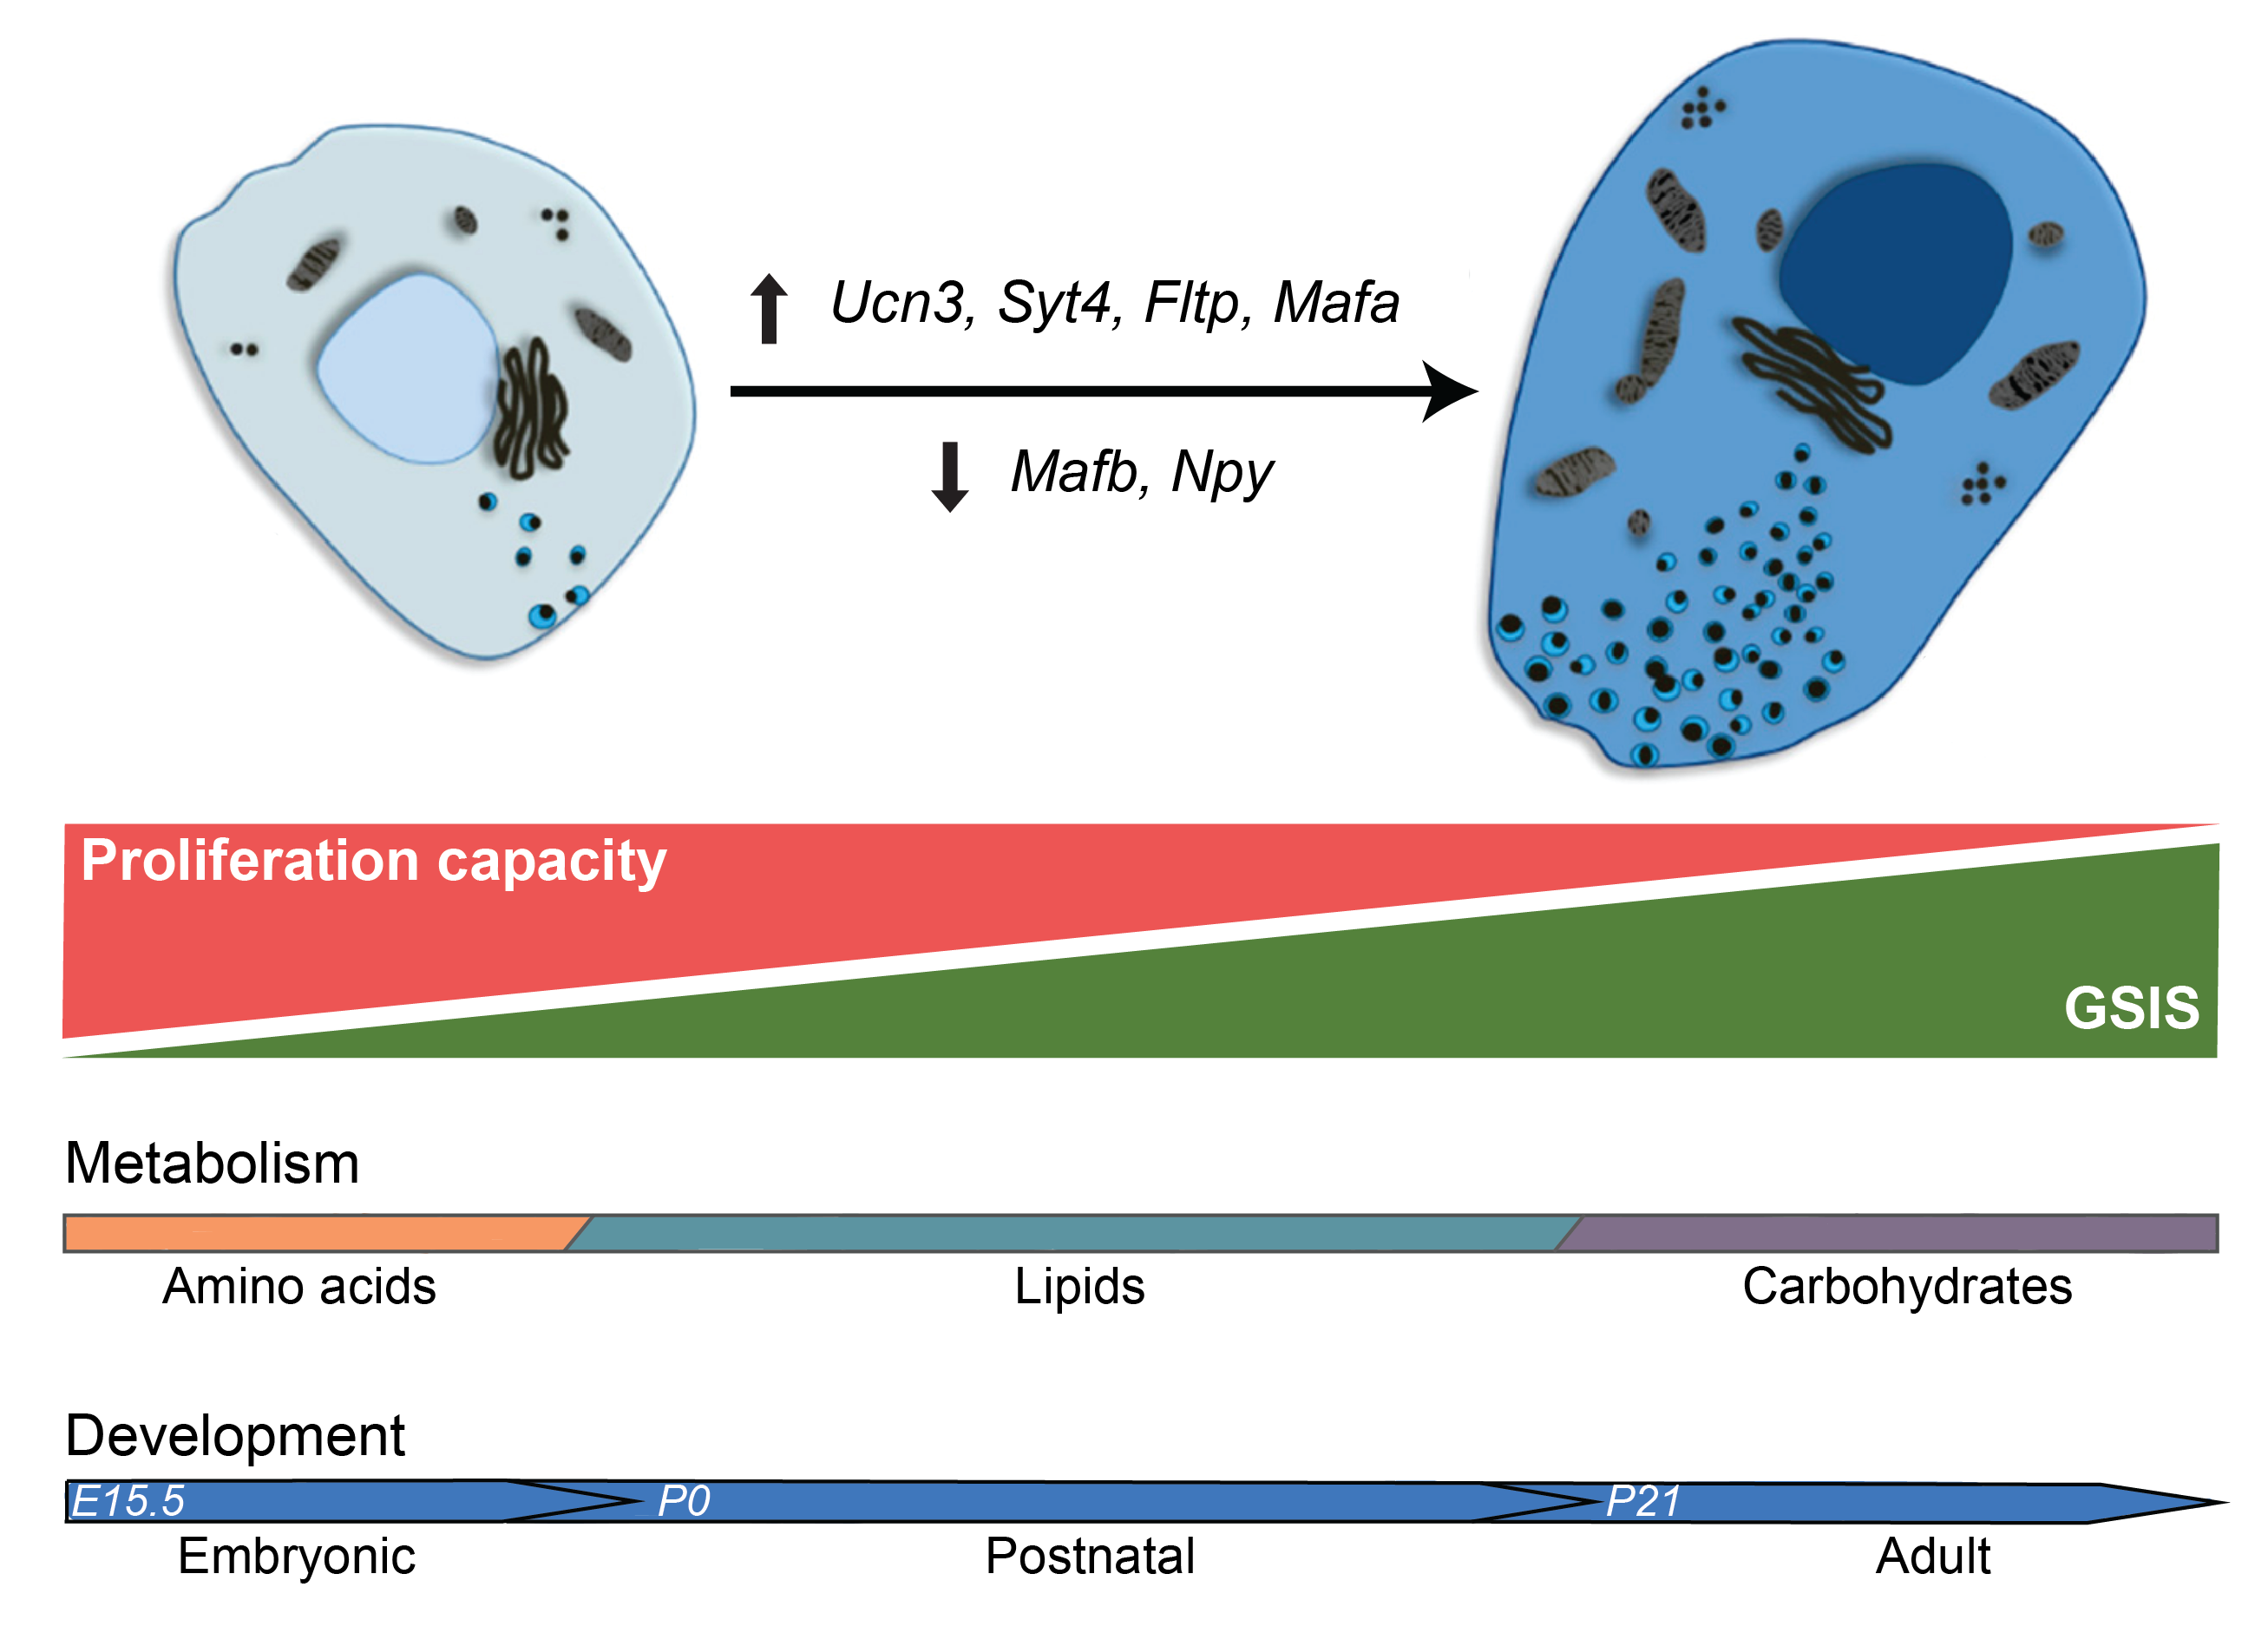
\includegraphics[width=8cm]{Chapter1/Fig/F1-16-01.png}
%     \caption[$\beta$-cell maturation process]{\textbf{$\beta$-cell maturation process.} \textit{This figure is adpated from }\textbf{\cite{salinno_-cell_2019}}. }
%     \label{fig:chp1_betamat}
% \end{wrapfigure}

\begin{figure}[t]
    \centering
    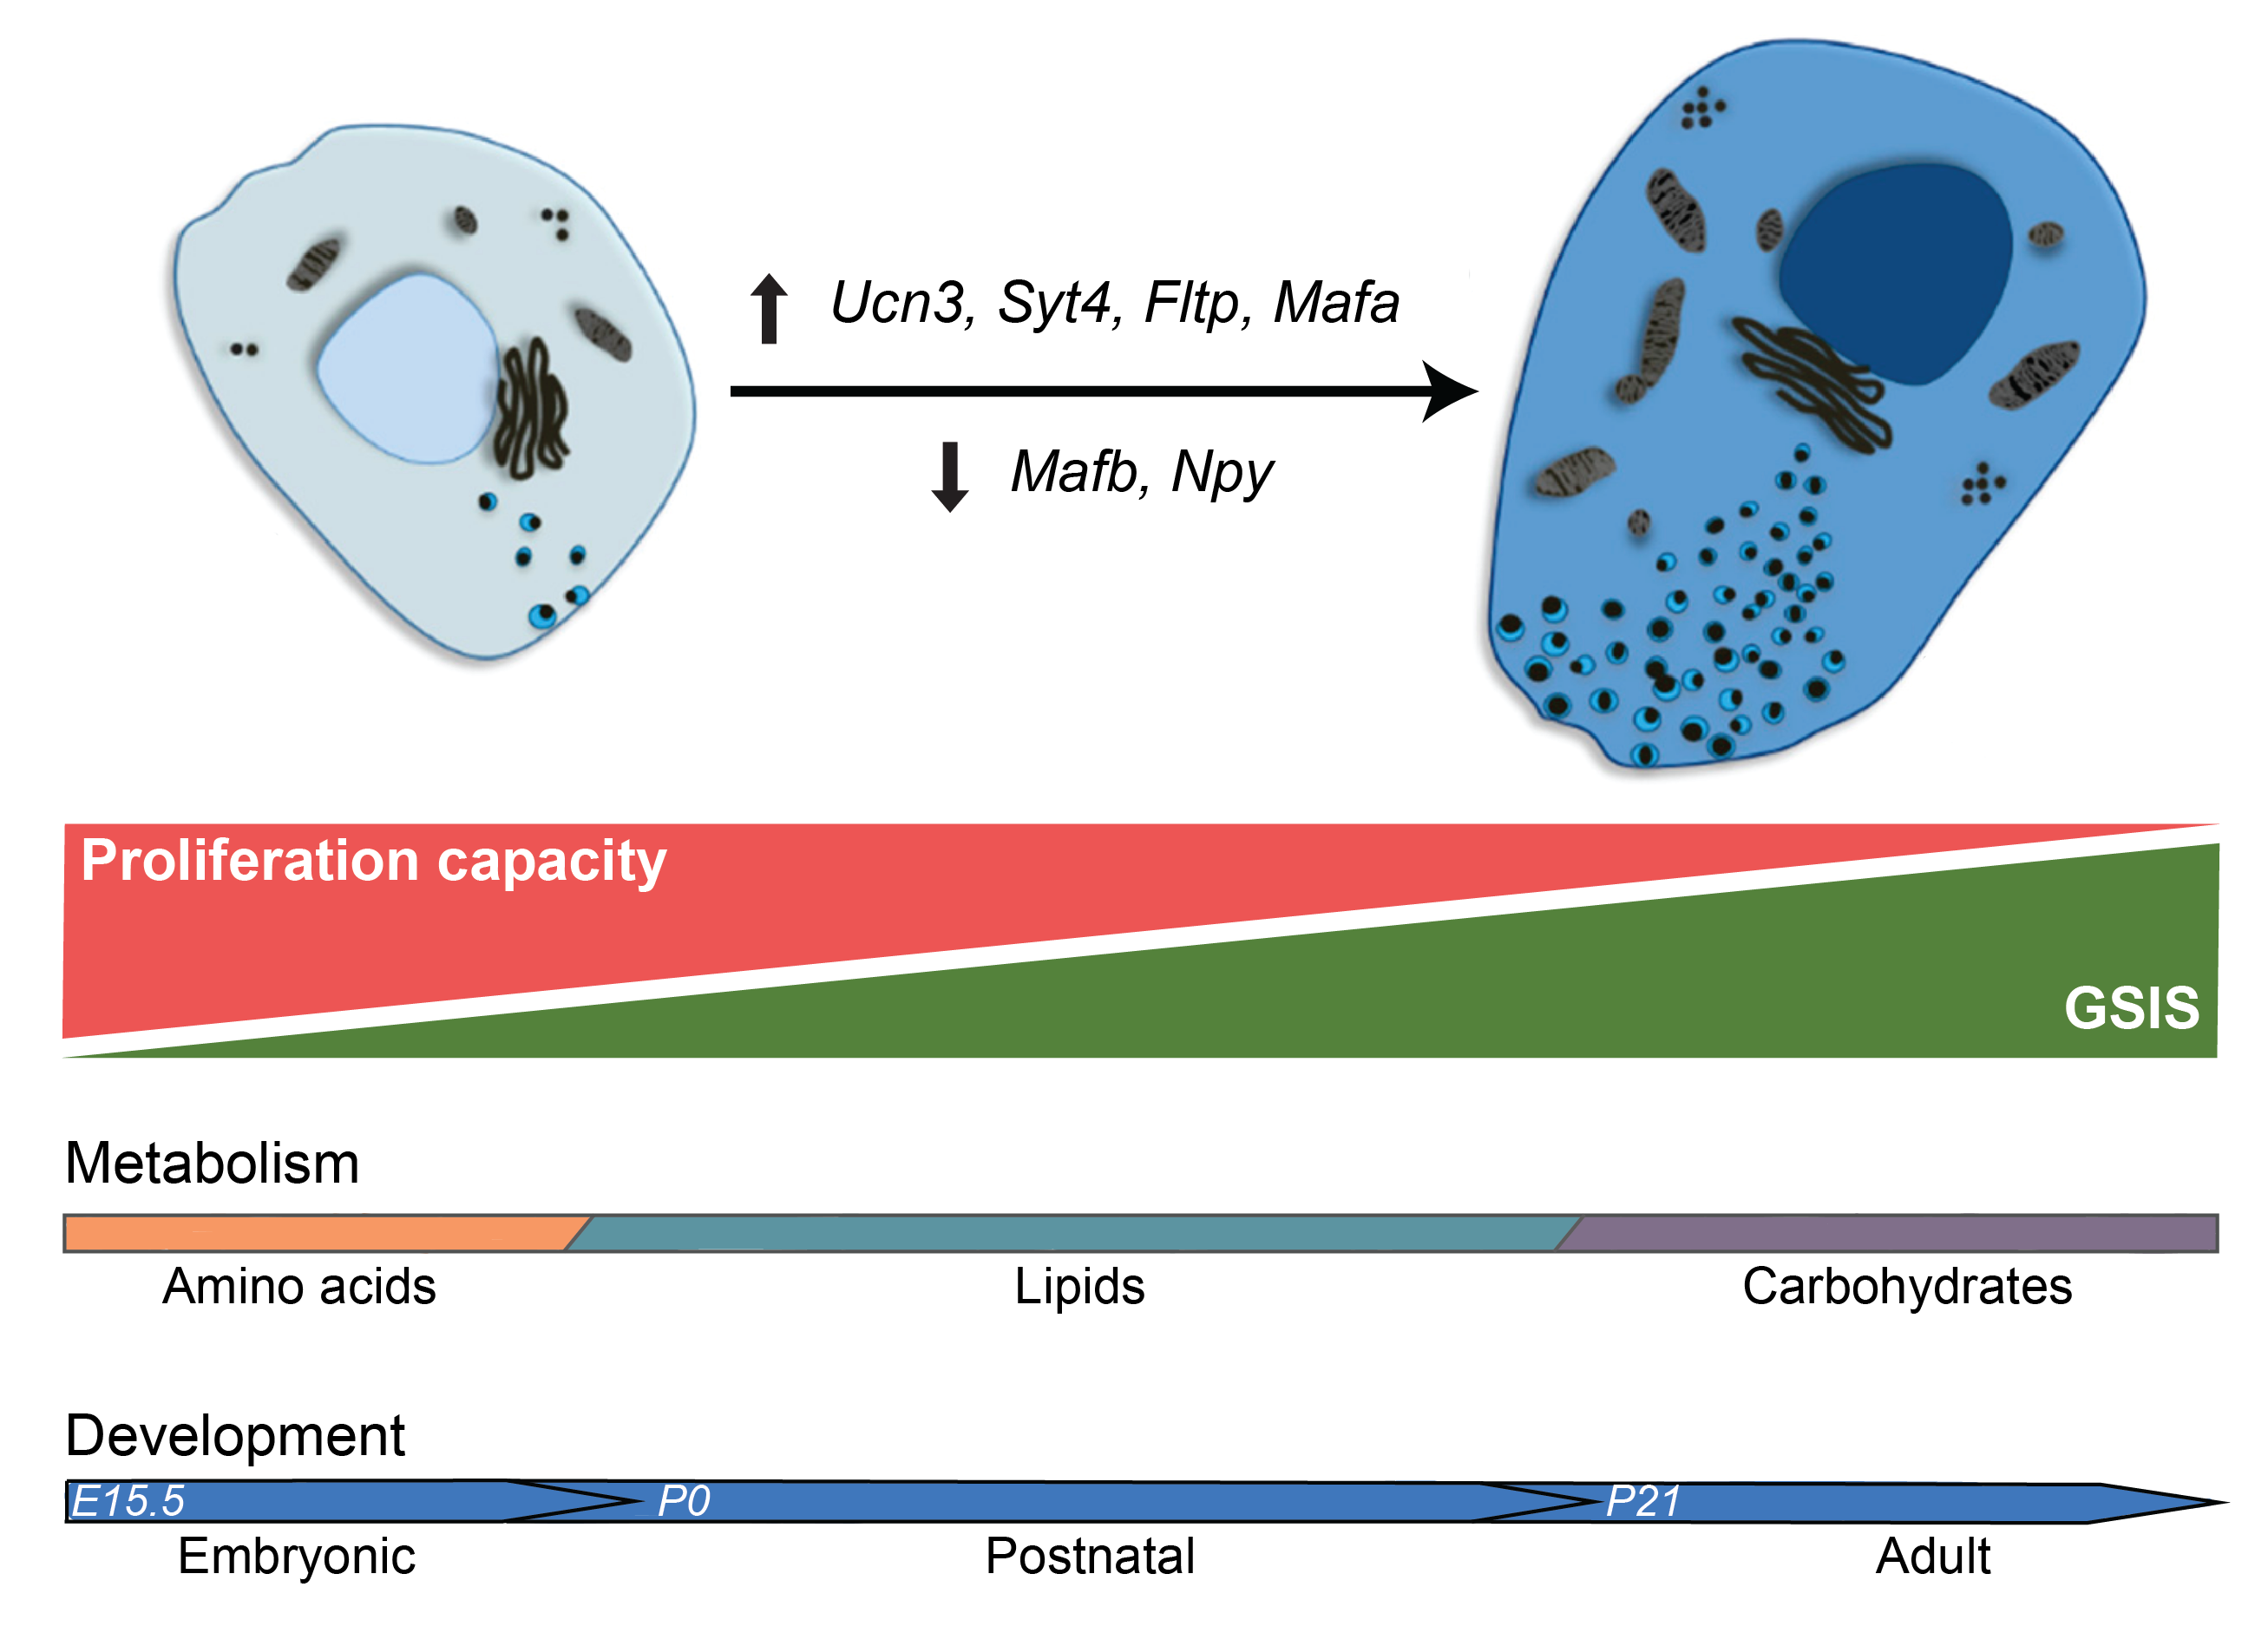
\includegraphics[width=12cm]{Chapter1/Fig/F1-16-01.png}
    \caption[]{\textit{This figure is adpated from }\textbf{\cite{salinno_-cell_2019}}.}
    \label{fig:chp1_betamat}
\end{figure}




\par Immature $\beta$-cells follow a bi-phasic pattern of maturation \textbf{\cite{salinno_-cell_2019, stolovich-rain_weaning_2015}}. The first wave starts right after birth and lasts until \textasciitilde 2 weeks, during which $\beta$-cells increase the expression of several key \glspl{tf} and associated machinery necessary to establish adult $\beta$-cell identity. At birth, all $\beta$-cells express key signature genes like \textit{Pdx1}, \textit{Neurod1}, \textit{Nkx2-2} and \textit{Nkx6-1}, which are important for the establishment and maintenance of $\beta$-cell identity. In addition, several other markers have also been identified which mark the early phase of functional maturation of $\beta$-cells: increased expression of \textit{Ucn3} \textbf{\cite{salinno_-cell_2019, blum_functional_2012}}, \textit{Syt4} \textbf{\cite{salinno_-cell_2019, huang_synaptotagmin_2018}}, \textit{Fltp} \textbf{\cite{salinno_-cell_2019, bader_identification_2016}}  and dramatic drop in levels of \textit{Npy} \textbf{\cite{salinno_-cell_2019, rodnoi_neuropeptide_2017}}. Among \glspl{tf}, \textit{Mafa} progressively substitutes \textit{Mafb} expression and further regulates expression of genes involved in glucose sensing and insulin secretion, thereby promoting functional maturation \textbf{\cite{salinno_-cell_2019}}. The switch from \textit{Mafb} %\st{(v-Maf avian musculoaponeurotic oncogene homolog B)} 
to \textit{Mafa} is an important step to activate the complete the $\beta$-cell specific program.
\\\\
The second wave of maturation occurs from about the third week of life until the weaning period involving dietary change from high-fat maternal milk to a high-carbohydrate chow diet. During this weaning phase, $\beta$-cells begin to exhibit improved glucose-stimulated insulin-secretion and glucose-induced replication, although the latter remains to be explained \textbf{\cite{salinno_-cell_2019,stolovich-rain_weaning_2015}}. This phase is characterized by $\beta$-cells differentially regulating metabolic pathways, involving a switch from \gls{mtor} to \gls{ampk} dependent signaling, which defines the mature functional landscape \textbf{\cite{salinno_-cell_2019,jaafar_mtorc1_2019}}. The dietary change associated with the weaning period also affects the secretion of incretin hormones, which enhance glucose-stimulated insulin secretion and modulate $\beta$-cell replication \textbf{\cite{campbell_pharmacology_2013}}.
% A recent review outlined emerging evidence about the developmental and homeostatic regulation of β-cell maturation and functional adaptation through collaboration between lineage-determining and signal-dependent TFs \textbf{\cite{wortham_transcriptional_2021}}.



% ********************************** % 1.3.3  **************************************
\subsection{Insulin Biosynthesis} %Section - 1.3.3
\label{sec:insbio}
%\colorbox{yellow}{missing text} \colorbox{pink}{missing figure}

The process of insulin synthesis is regulated by glucose, which stimulates the transcription of insulin gene and increases insulin \glslink{mrna}{mRNA} expression. Humans have a single insulin gene, \textit{INS}, whereas, rodents have two \textit{Ins1} and \textit{Ins2}. The insulin gene is transcribed into preproinsulin \glslink{mrna}{mRNA} which has a long half-life and is the most abundant transcript in $\beta$-cells. Upon glucose stimulation, the preproinsulin \glslink{mrna}{mRNA} are transported to the \glslink{er}{ER} and the translation starts immediately. In the ER, signal peptidase cleaves the signal peptide and converts the preproinuslin to proinsulin. Further, disulfide bridges are formed, and the proinsulin is trafficked from the ER through the Golgi and the \textit{trans-}Golgi network into \glspl{sg}. Within the granules, proinsulin is processed via the prohormone convertases PC1/3 (humans) and PC2 (rodents), which cleave the C-peptide. Thereby, both, the mature insulin and C-peptide are stored in the same \gls{sg}. Mature insulin is stored as hexameric insulin / Zn\textsuperscript{2+} crystals in the \glspl{sg} and is released by regulated exocytosis \textbf{(Fig. \ref{fig:chp1_ins_bio})} \textbf{\cite{vasiljevic_making_2020,tokarz_cell_2018}}. Along with insulin, the C-peptide is also secreted in equimolar concentrations, and thus represents a direct measure of endogeneous insulin \textbf{\cite{venugopal_biochemistry_2024}}. 

\begin{figure}[t]
    \centering
    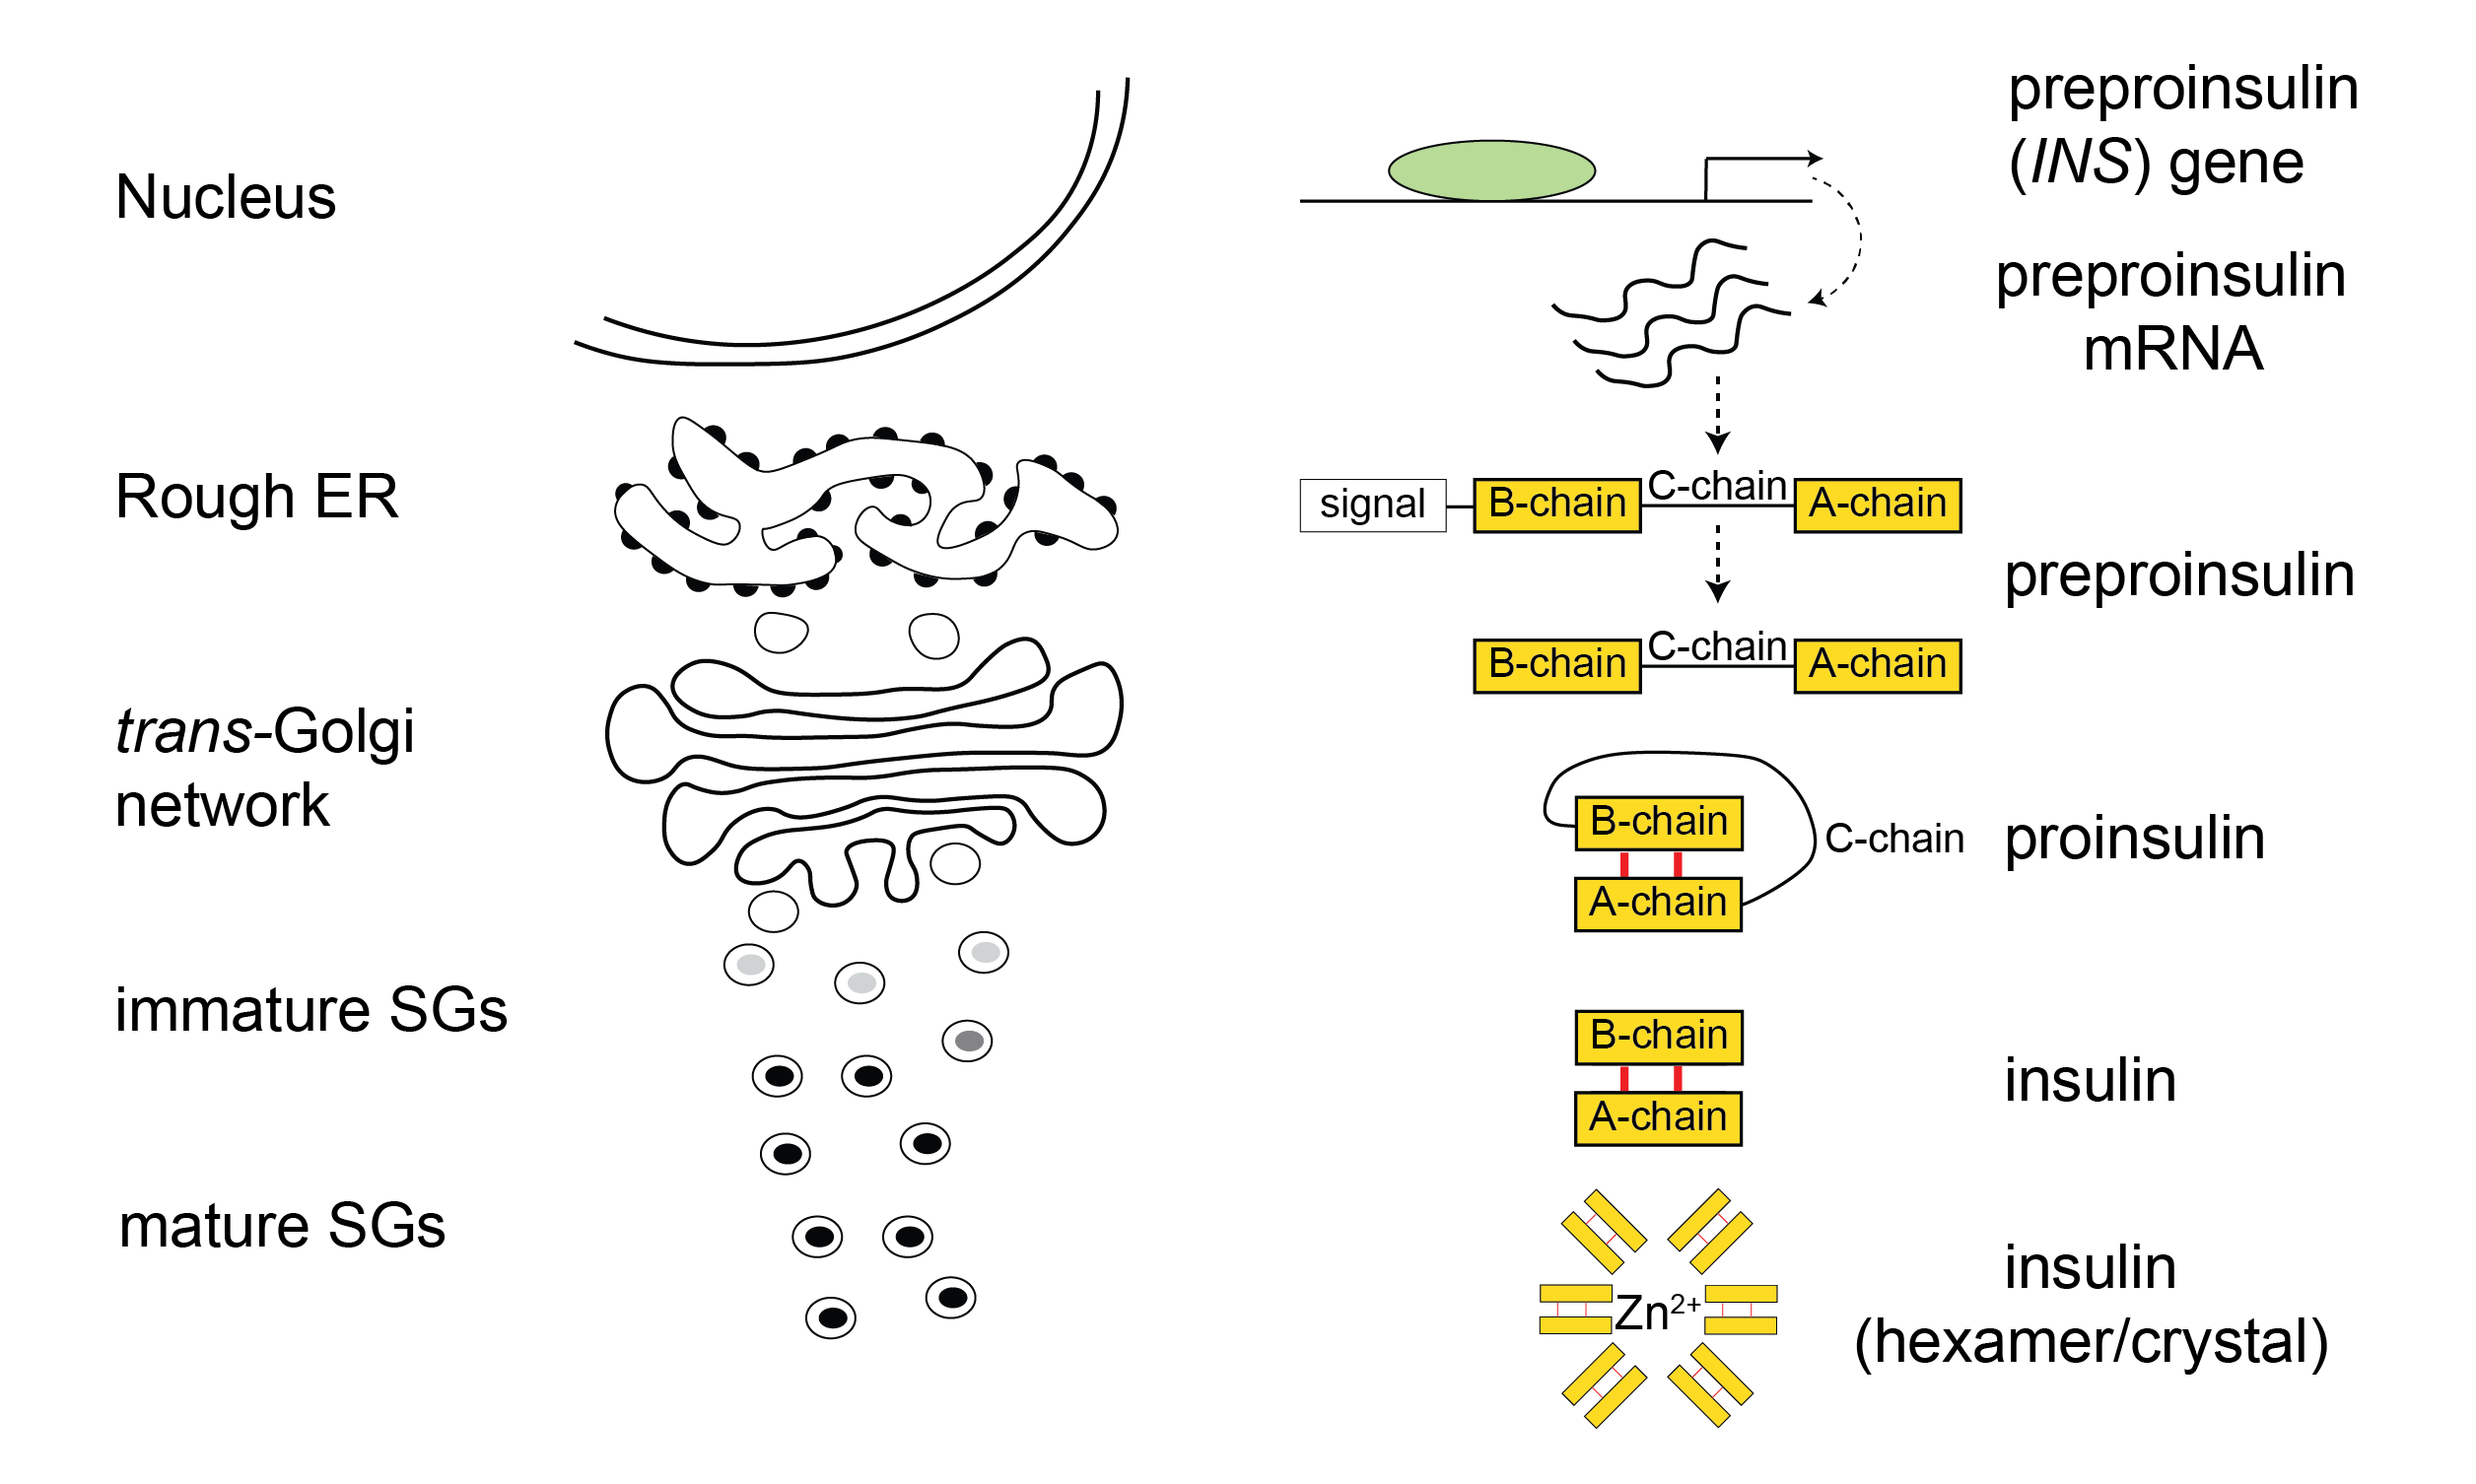
\includegraphics[width=\linewidth]{Chapter1/Fig/F1-9-01.png}
    \caption[Insulin biosynthesis in $\beta$-cells]{\textbf{Overview of insulin biosynthesis along the granule secretory pathway.} Preproinsulin \glslink{mrna}{mRNA} is transcribed and translated into preproinsulin peptide. This peptide is processed to its mature form as it transits the ER and \textit{trans-}Golgi network and is ultimately stored as hexmeric insulin / Zn\textsuperscript{2+} crystals within mature secretory granules. Abbreviations: ER, endoplasmic reticulim; SG, secretory granule. \textit{This figure is adapted from \textbf{\cite{tokarz_cell_2018}}.}}
    \label{fig:chp1_ins_bio}
\end{figure}

% ********************************** % 1.2.5  **************************************
\subsection{Glucose-Stimulated Insulin Secretion} %Section - 1.2.5
\label{sec:gsis}

%\colorbox{pink}{missing figure} \colorbox{green}{text clean-up} \\
% \subsubsection{Triggering \& Amplifying Pathways}
Insulin, secreted by pancreatic $\beta$-cells in response to elevated blood glucose levels, is the central anabolic hormone promoting nutrient utilization and energy storage of metabolic fuel \textbf{\cite{slack_developmental_1995}}. The molecular process wherein hormone release is triggered by a stimulus is called stimulus-secretion coupling.  The release of insulin by a post-prandial increase in glucose concentrations is termed as \gls{gsis}, and is the most critical aspect of $\beta$-cell functionality \textbf{\cite{ashcroft_stimulussecretion_1994}}.  Impaired \gls{gsis} is an early marker of $\beta$-cell dysfunction and contributes to the pathogenesis of metabolic disorders such as obesity and \gls{t2d} \textbf{\cite{jensen_metabolic_2008}}. The canonical pathway for \gls{gsis} consists of two distinct components – triggering pathway and amplifying signals \textbf{(Fig. \ref{fig:chp1_gsis} A)} \textbf{\cite{henquin_triggering_2000}}. 
\\
\par In the triggering pathway, the pancreatic $\beta$-cells act as a glucose sensing machinery with the help of \gls{glut} embedded in their plasma membranes and respond to changes in blood glucose levels. \gls{glut}2, encoded by \textit{Slc2a2}, is the predominant glucose transporter in rodent β-cells \textbf{\cite{mcculloch_glut2_2011,van_de_bunt_tale_2012}} and facilitates rapid entry of glucose into the cell, owing to low affinity and high capacity nature. In human pancreatic islets and $\beta$-cells, \gls{glut}1 encoded by \textit{SLC2A1} and \gls{glut}3 encoded by \textit{SLC2A3} are the primary glucose transporters \textbf{\cite{mcculloch_glut2_2011}}. After trans-membrane transport (via facilitated diffusion), glucose is rapidly phosphorylated to \gls{g6p} by \gls{gck} \textbf{\cite{campbell_mechanisms_2021,matschinsky_central_2019}}. \gls{gck}, a specialized glucose phosphorylation enzyme, is a hexokinase isozyme and is expressed in both, rodent and human $\beta$-cells \textbf{\cite{campbell_mechanisms_2021}}. Compared to the other three members of the hexokinase gene family, \gls{gck} has a lower affinity for glucose (\textit{K\textsubscript{m}} \textasciitilde 1.5-12 mM) and lacks feedback inhibition by \gls{g6p} \textbf{\cite{matschinsky_central_2019}}. Taken together, \gls{gck} along with \gls{glut} 1/2 endows $\beta$-cells with appropriate kinetics to quickly sense changes in glucose levels. High glycerol phosphate shuttle, pyruvate dehydrogenase, and pyruvate carboxylase activities, combined with low pentose-phosphate shunt, lactate dehydrogenase, plasma membrane monocarboxylate transport, and glycogen synthase activities constrain \gls{g6p} to being metabolized through oxidative glycolysis \textbf{\cite{matschinsky_central_2019}}, resulting in the increase of \glslink{atp}{ATP} levels and cytosolic ATP / \glslink{adp}{ADP} ratio within the cell \textbf{\cite{henquin_triggering_2000}}. $\beta$-cells are equipped with -

\begin{figure}[t]
    \centering
    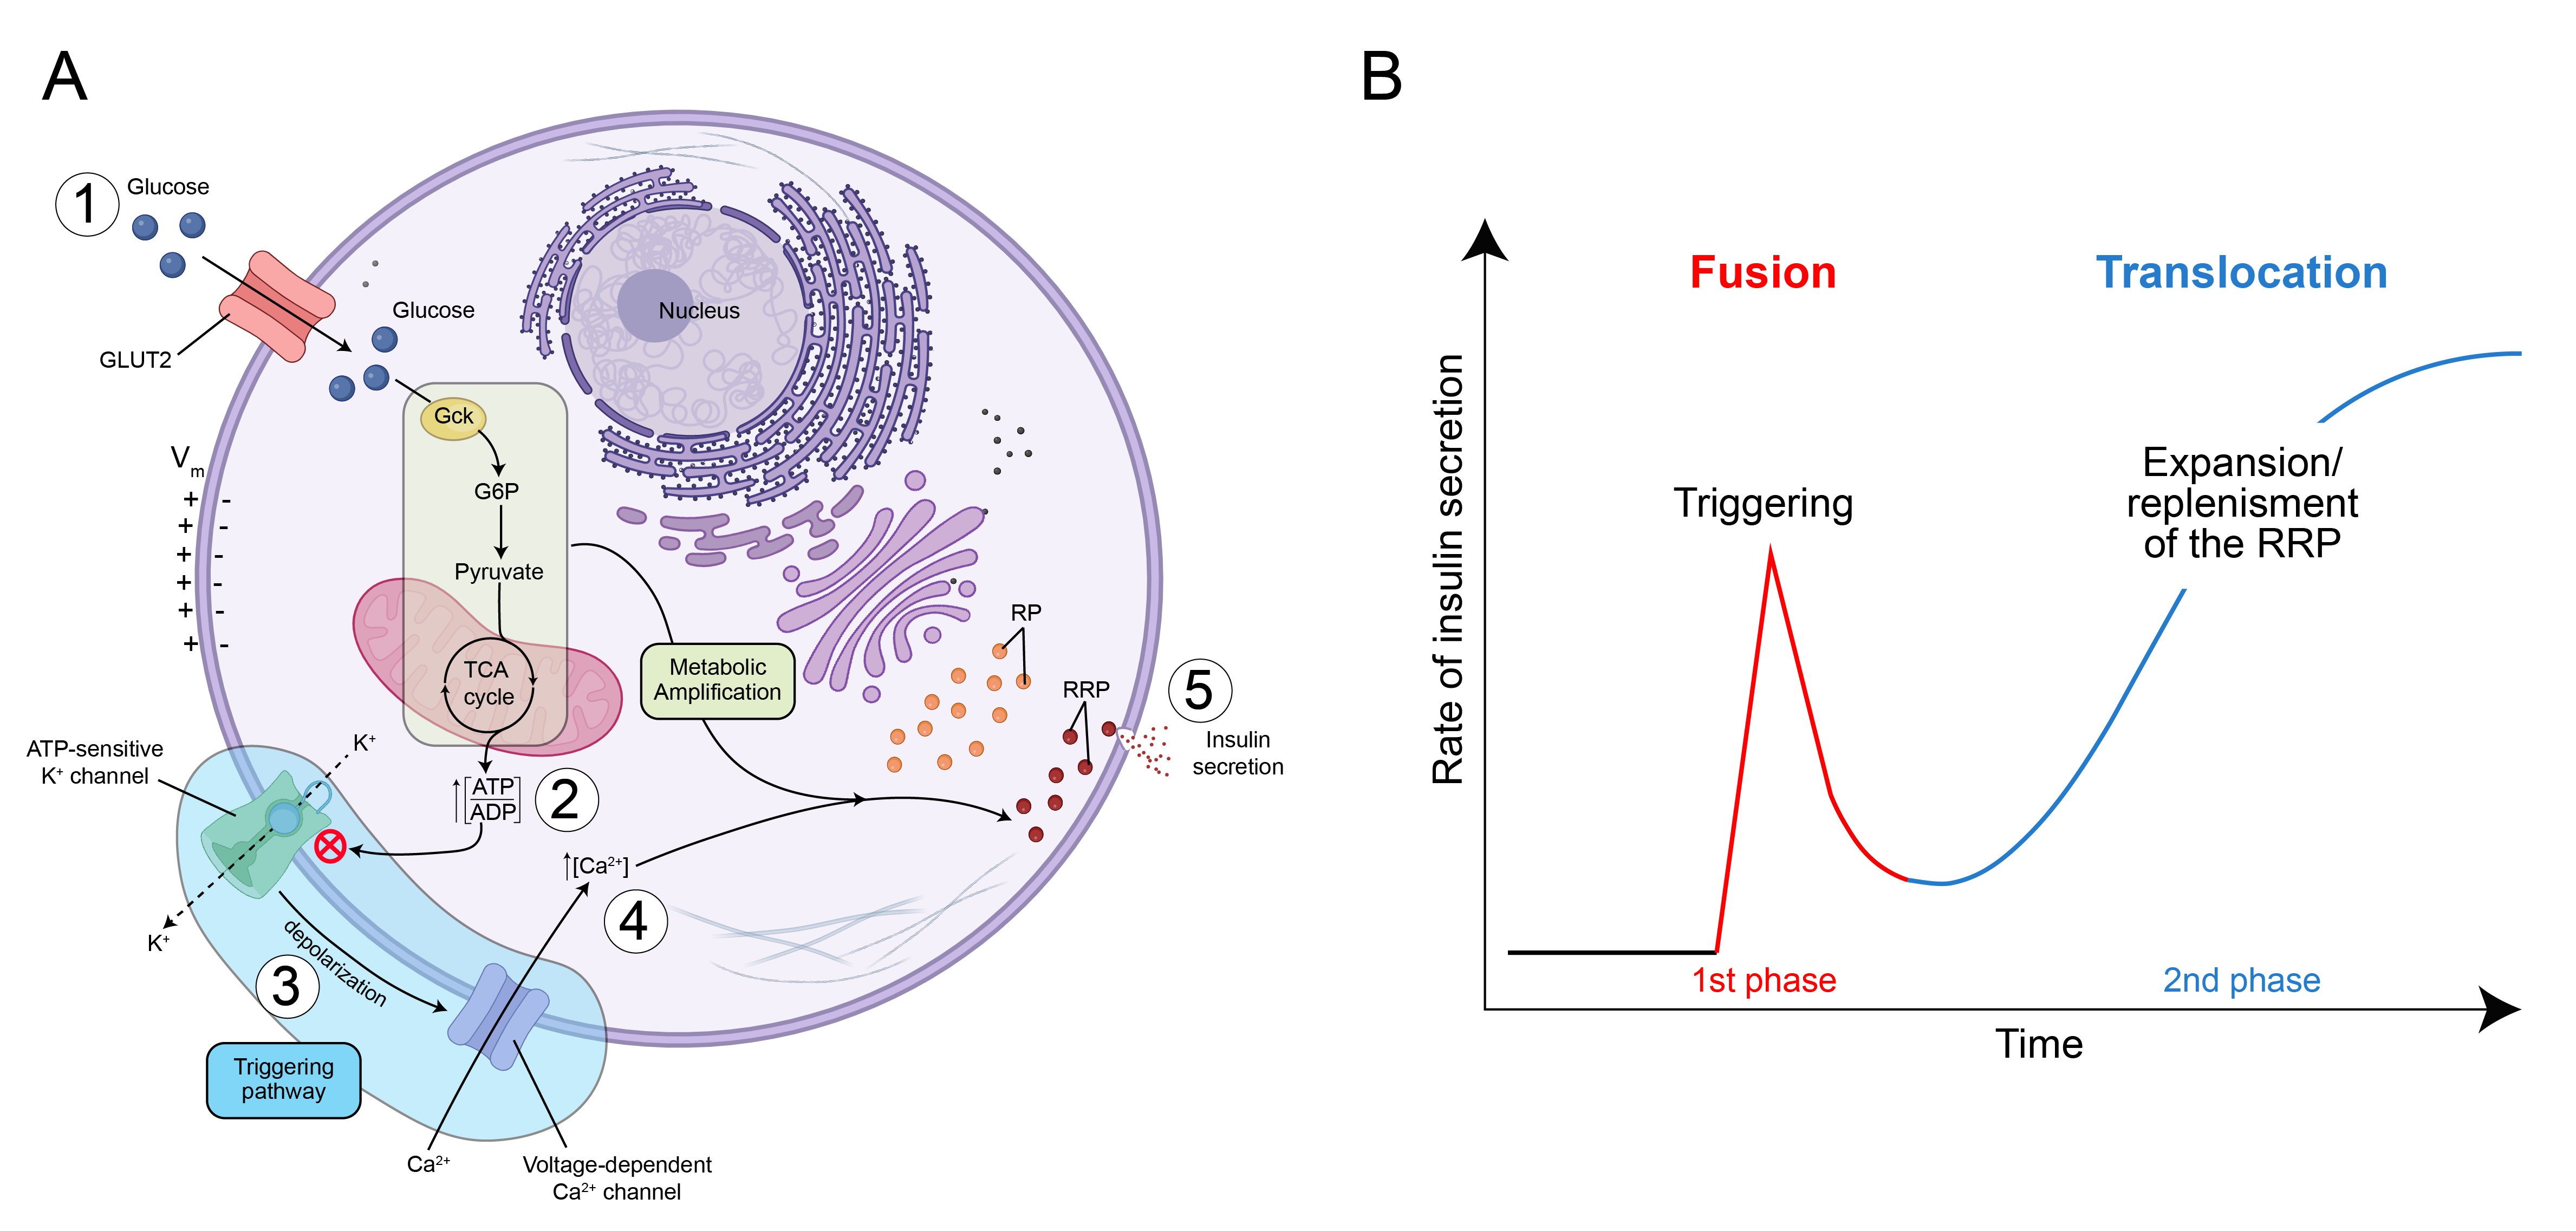
\includegraphics[width=\linewidth]{Chapter1/Fig/F1-11-01.png}
    \caption[Glucose-stimulated insulin secretion in $\beta$-cells]{\textbf{Schematic Overview of \gls{gsis} in mature $\beta$-cells. (A)} The entry of glucose into $\beta$-cells is facilitated by \gls{glut}2 in rodents. Upon entry, glucose is phosphorylated and then metabolized through oxidative glycolysis resulting in the increase of \glslink{atp}{ATP} / \glslink{adp}{ADP} ratio. This increase leads to the closure of the \glslink{katp}{K\textsubscript{ATP}} channels which depolarizes the membrane to activate voltage-dependent Ca\textsuperscript{2+} channel and allows the influx of Ca\textsuperscript{2+}. This constitutes the triggering pathway resulting in the docking and fusion of insulin granules and subsequent insulin release. Additional signals, through metabolism of glucose, increases the release competency of the insulin granules and amplifies the secretory response. \textbf{(B)} A schematic depicting the glucose-induced biphasic insulin secretion. Stimulation by high glucose concentrations initially causes a rapid insulin secretion followed by a reduction and gradual resurgence. The first phase involves fusion of the insulin granules at the plasma membrane, and the second phase is marked by granule translocation from RP to RRP yielding the expansion and/or replenishment of the RRP. Abbreviations: GLUT2, glucose transporter 2; Gck, glucokinase; G6P, glucose-6-phosphate; TCA, tricarboxylic acid; RP, reserve pool; RRP, readily releasable pool. \textit{This figure is adapted from }\textbf{\cite{campbell_mechanisms_2021,aizawa_rab27a_2005}}. \textit{Reproduced with permission from Springer Nature.} Created with \href{https://www.biorender.com/}{Biorender.com}.}  
    \label{fig:chp1_gsis}
\end{figure}


- \gls{katp} channels that undergo closure in an ATP-dependent manner, thereby causing the accumulation of K\textsuperscript{+} ions within the cell and ultimately leading to depolarization of the plasma membrane. This, in turn, results in the opening of \gls{vdcc}, allowing entry of calcium (Ca\textsuperscript{2+}) ions into the cell down the electrochemical gradient by facilitated diffusion. In addition, Ca\textsuperscript{2+} released from intracellular stores also contribute to the rise of cytosolic Ca\textsuperscript{2+} concentration \textbf{\cite{yang_ionic_2014}}. The increase in intracellular Ca\textsuperscript{2+}, which is the indispensable signal, triggers exocytosis. The insulin-containing \glspl{sg} interact with the SNARE-complex proteins resulting in docking of the \glspl{sg} at correct plasma membrane sites, leading to fusion and insulin release \textbf{(Fig. \ref{fig:chp1_gsis} A)} \textbf{\cite{jewell_exocytosis_2010,chatterjee_bhowmick_conventional_2021}}.   %fuse with the plasma membrane and release insulin into the extracellular space. 
The triggering pathway was also previously referred to as the \textbf{ \gls{katp}-dependent pathway}.
\\\\
%While the triggering signal is sufficient to initiate insulin secretion, it is poorly effective \textbf{\cite{henquin_pathways_2004}}. 
The metabolism of glucose generates additional signals that serve to fine-tune the action of increase in intracellular Ca\textsuperscript{2+} concentrations. This mechanism was shown to work independent of the \gls{katp} channels \textbf{\cite{sato_dual_1992,gembal_evidence_1992}}, and was therefore termed as \textbf{\gls{katp}-independent pathway}. It is now referred to as the \textbf{metabolic amplifying pathway} \textbf{(Fig. \ref{fig:chp1_gsis} A)} \textbf{\cite{henquin_triggering_2000,henquin_pathways_2004,henquin_regulation_2009}}.  This pathway depends on the initial triggering signal of Ca\textsuperscript{2+} influx and increases the release competency of insulin granules thereby augmenting insulin secretion in a glucose-concentration-dependent manner \textbf{\cite{henquin_triggering_2000,kalwat_mechanisms_2017}}. The metabolic amplifying pathway accounts for $\sim$60-70\% of the total insulin secreted \textbf{\cite{henquin_regulation_2009}}, and can optimize the secretory response to non-glucose stimuli in addition to glucose \textbf{\cite{henquin_triggering_2000,kalwat_mechanisms_2017,zhao_-hydrolase_2015,tengholm_camp_2017,han_glutamate_2021}}. This amplifying pathway can also be observed in models of \gls{katp} channel knockouts which result in constant depolarization of the $\beta$-cell \textbf{\cite{nenquin_both_2004,miki_defective_1998,ravier_glucose_2009}}. The exact mechanisms behind the amplifying pathway remain to be elucidated and several metabolites and their sensors that participate in amplification have been proposed \textbf{\cite{kalwat_mechanisms_2017}}.%In addition to the glucose-derived metabolites, the metabolic amplifying pathway also include non-metabolic stimuli. 
\\
% \par The secretory granules stored within the $\beta$-cell cytoplasm travel along the dense microtubule network to reach the cell periphery. At the periphery, actin reorganization on account of glucose stimulation allows the granules to access the plasma membrane for subsequent docking and fusion. The interaction with SNARE-complex proteins docks the secretory granules at the correct membrane site leading to fusion and insulin release \textbf{\cite{jewell_exocytosis_2010,chatterjee_bhowmick_conventional_2021}}.
% \\

% \begin{wrapfigure}{l}{0.5\textwidth}
% \centering
% 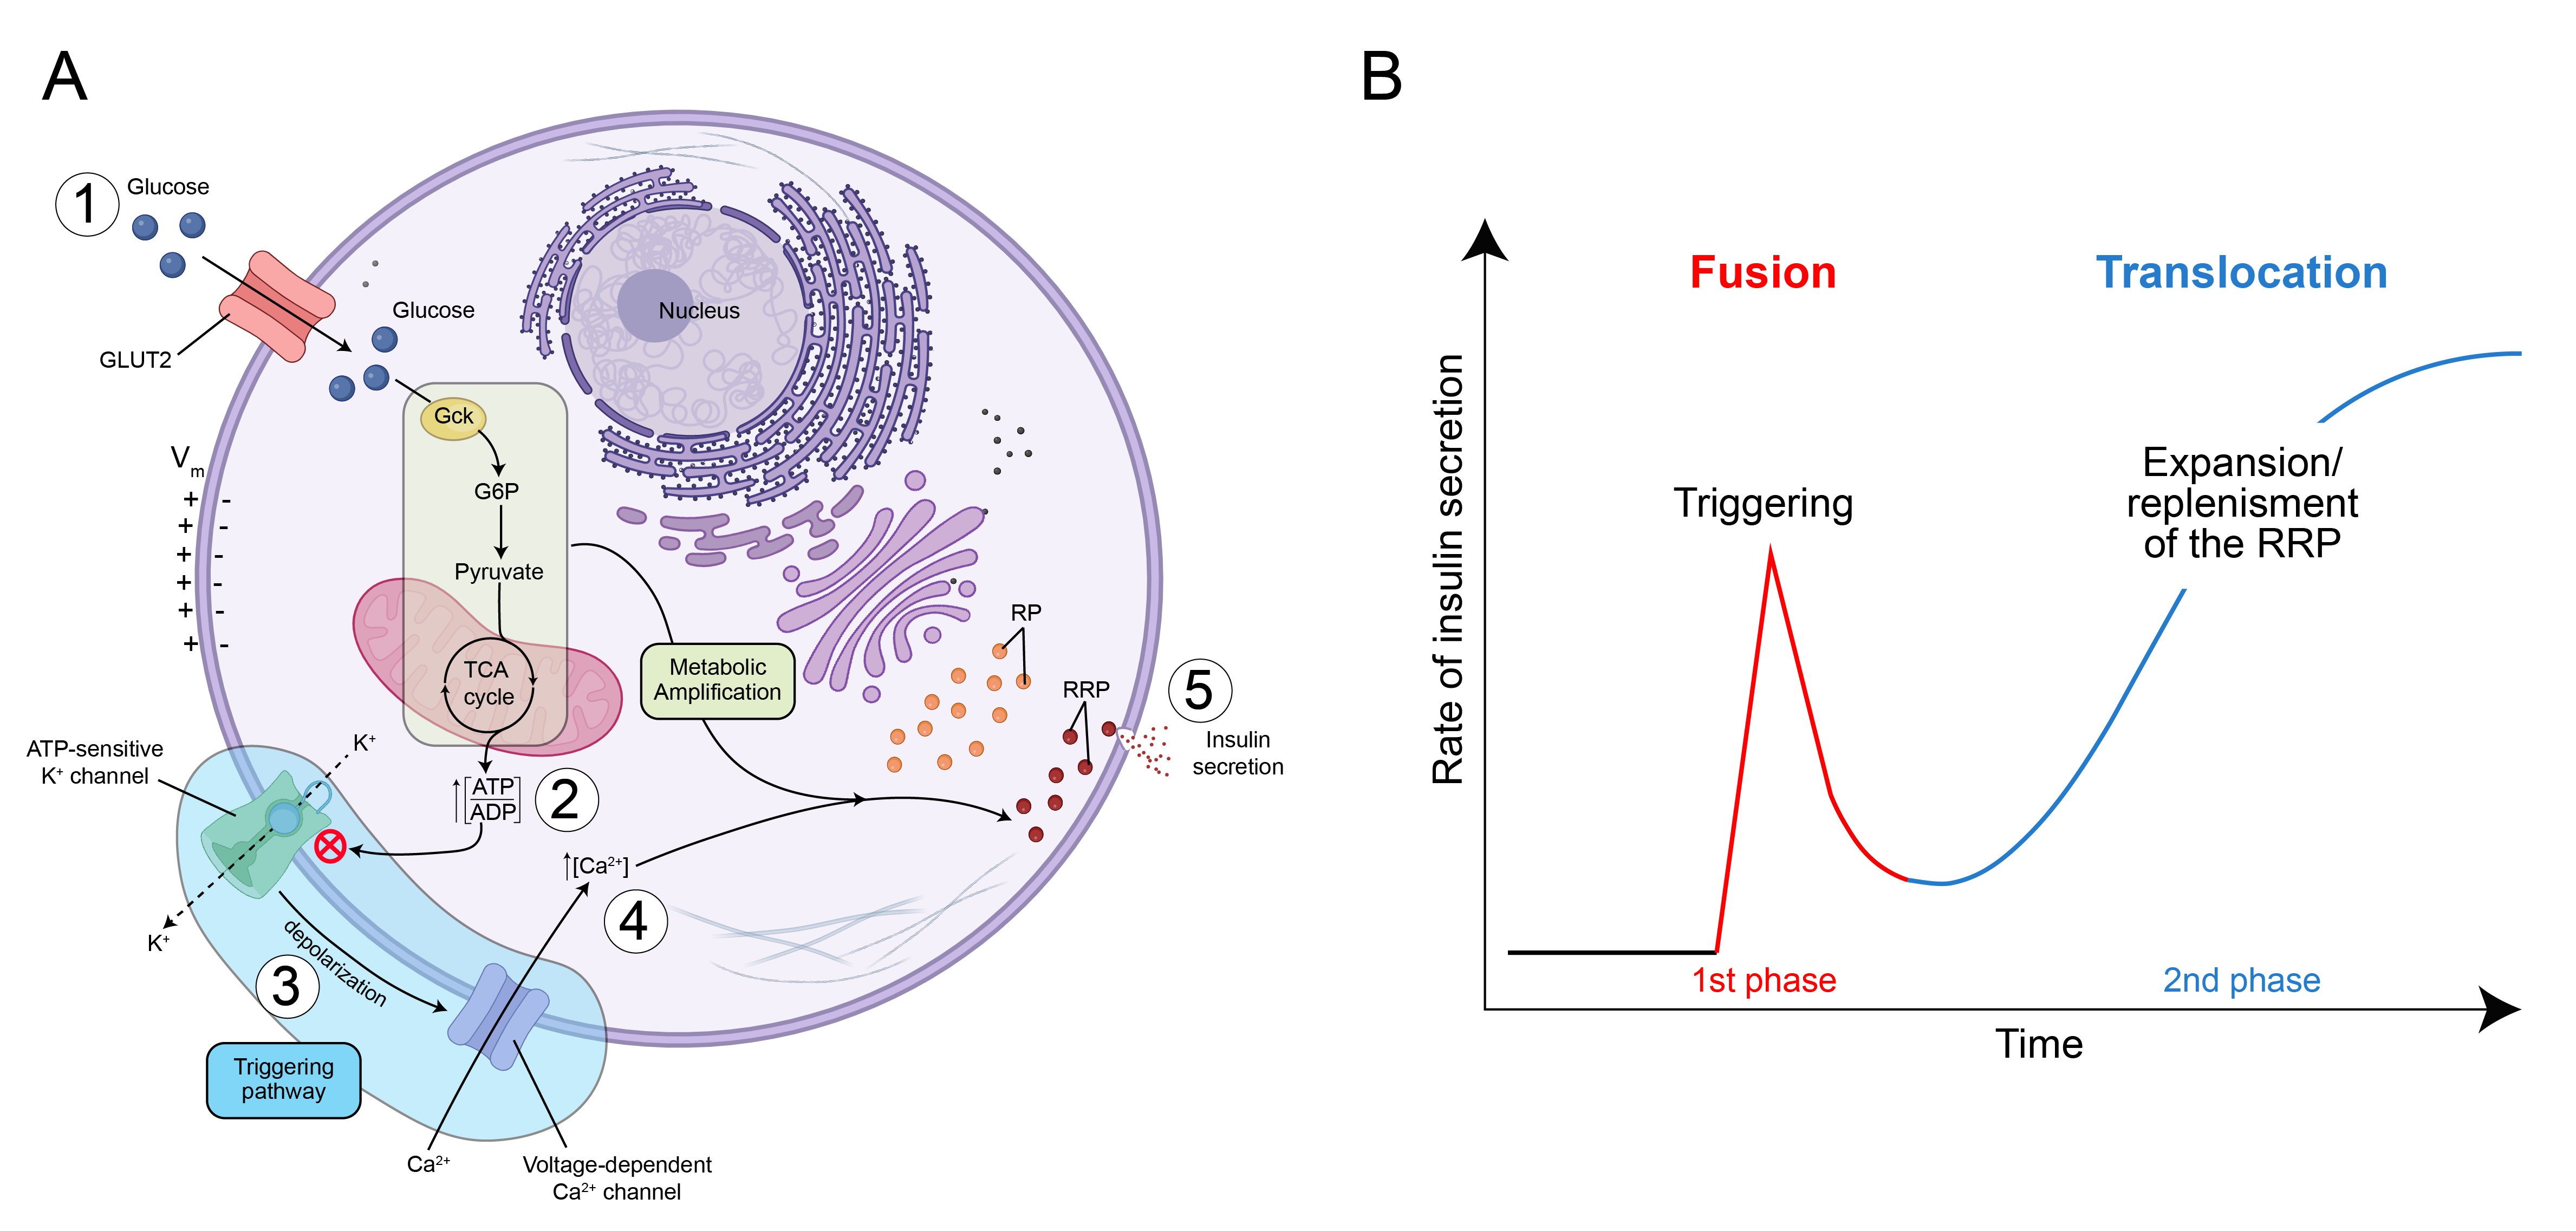
\includegraphics[]{Chapter1/Fig/F1-11-01.png}
% \caption[]{}
% \label{label}
% \end{wrapfigure}

\par \gls{gsis} follows a characteristic biphasic pattern – a peak-shaped first phase followed by a coordinated, pulsatile second phase \textbf{(Fig. \ref{fig:chp1_gsis} B)} \textbf{\cite{ashcroft_diabetes_2012,grodsky_threshold_1972,komatsu_glucosestimulated_2013}}. Researchers have proposed that the biphasic nature reflects the existence of distinct pools of \glspl{sg} within the $\beta$-cells, and has also been confirmed by a \glslink{fret}{FRET}-based study \textbf{\cite{ashcroft_diabetes_2012,takahashi_snare_2010}}. The rapid but transient first phase lasts $\sim$5-20 minutes after glucose stimulus, during which pre-docked insulin-containing \glspl{sg} near the Ca\textsuperscript{2+} channels, called \gls{rrp} undergo exocytosis, thereby giving a short, boosted secretion curve. The triggering pathway is mainly responsible for this first phase of \gls{gsis} \textbf{\cite{kalwat_mechanisms_2017,campbell_mechanisms_2021}} %and causes the release of about 1\% of  the RRP \textbf{\cite{campbell_mechanisms_2021}}. 
In contrast, the second phase exhibits a sustained secretion at a lower rate as new granules from the cell-internal \gls{rp} replenish the \gls{rrp} by physical translocation to the plasma membrane before exocytosis. Therefore, Komatsu et. al. \textbf{\cite{komatsu_glucosestimulated_2013}} proposed viewing the biphasic insulin release as \textbf{fusion and replacement}. The metabolic amplifying pathway associates with this second phase of \gls{gsis} \textbf{\cite{kalwat_mechanisms_2017,campbell_mechanisms_2021}}. Although, there is sufficient evidence to demonstrate that amplification is involved during both phases of insulin secretion \textbf{\cite{mourad_metabolic_2010,mourad_metabolic_2011}}. It is important to note that the biphasic insulin secretion is a conceptual framework in order to experimentally dissect insulin secretion, as it can be observed in response to very high glucose concentration applied to isolated islets in perifusion assays and likely does not occur in response to meal feeding \textit{in vivo} \textbf{\cite{aizawa_rab27a_2005}}.\\

% % ********************************** % 1.2.6  **************************************
% \subsection{Regulation of GSIS} %Section - 1.2.6
% \label{sec:reggsis}
% \colorbox{pink}{missing figure} \colorbox{green}{text clean-up} \\

\par Besides glucose, insulin secretion by $\beta$-cells can also be regulated by insulinotropic gut hormones like \glslink{glp1}{GLP-1} \textbf{\cite{meloni_glp-1_2013,carlessi_glp-1_2017,macdonald_multiple_2002}} and \glslink{gip}{GIP} \textbf{\cite{seino_gip_2010,christensen_glucose-dependent_2011,irwin_therapeutic_2009}}, amino acids \textbf{\cite{newsholme_amino_2006,newsholme_nutritional_2012}}, fatty acids \textbf{\cite{poitout_fatty_2018,cen_fatty_2016,jezek_fatty_2018,chueire_effect_2020}}. Apart from these factors, insulin secretion can also be regulated by other hormones \textbf{\cite{cheng_follicle-stimulating_2023}}, neural inputs via the autonomic \textbf{\cite{thorens_brain_2011, komatsu_glucosestimulated_2013}} and central nervous systems \textbf{\cite{ruud_neuronal_2017}} and neurotransmitters \textbf{\cite{rodriguez-diaz_neurotransmitters_2014}}, reflecting a complex interplay between the various body systems in maintaining glucose homeostasis. 

% also respond to other nutrients such as amino acids and fatty acids, leading to fuel-induced insulin secretion. In addition, other hormones and neurotransmitters can also modulate insulin secretion by β-cells.\st{The following section discusses a few of these of regulators of insulin secretion:}

% \subsubsection{Gut Hormones}
% The gut hormones, also known as incretins, are secreted by specialized enteroendocrine cells in the bowel and play crucial roles in regulating glucose homeostasis and other metabolic functions. The incretins exhibit “incretin effect” to stimulate insulin secretion and are responsible for ~ 50 -70\% of the insulin response to glucose. The two main incretin hormones, which are insulinotropic, are:

% \begin{enumerate}
%     \item\textbf{Glucagon-like peptide 1 (GLP-1)}\\
%     GLP-1 affects insulin secretion in a glucose-dependent manner and regulates factors involved in KATP-dependent insulin secretion. GLP-1 binds to GLP-1R and depolarizes the membrane potential by blocking the K-ATP channels, which is a crucial step in the insulin secretion pathway. Further, GLP-1 potentiates the opening of VDCCs by altering the permeability of these channels thereby allowing for more Ca2+ influx and greater insulin secretion \textbf{\cite{meloni_glp-1_2013}}. However, in absence of glucose, GLP-1 has little to no effect on insulin secretion. Besides, GLP-1 has also been shown to modulate β-cell metabolism upon chronic exposure \textbf{\cite{carlessi_glp-1_2017}} and induce β-cell mass expansion by promoting proliferation and inhibiting apoptosis pathways \textbf{\cite{macdonald_multiple_2002}}. 
%     \item\textbf{Glucose-dependent insulinotropic polypeptide (GIP)}\\GIP exerts its insulinotropic effects in a similar fashion to GLP-1 and binds to its specific receptor GIPR on β-cells. GIP seems to be a physiological bi-functional blood glucose stabilizer. GIP potentiates insulin secretion in a glucose-dependent manner whereas it enhances postprandial glucagon response \textbf{\cite{seino_gip_2010, christensen_glucose-dependent_2011}}. Furthermore, GIP also facilitates fat deposition in adipose tissues, and promotes bone formation \textbf{\cite{seino_gip_2010}}. In type-2 diabetic individuals, GIP has impaired effect on insulin secretion due to the downregulation of GIPR \textbf{\cite{irwin_therapeutic_2009}}.

% \end{enumerate}

% \subsubsection{Amino Acids}
% Amino acids exert influence on insulin secretion via their mitochondrial metabolism in β-cells to generate metabolic coupling factors. One such factor, ATP, generated via the oxidation of amino acids, suppresses \gls{katp} channels and activates \glspl{vdcc}, leading to the exocytosis of insulin granules. %The amino acid, L-arginine is considered a powerful secretagogue as well as an essential synergistic compound for nutrient-dependent insulin secretion \textbf{\cite{newsholme_nutritional_2012}}. 
% Certain amino acids also play a crucial role in nutrient-sensing signaling \textbf{\cite{newsholme_nutritional_2012}} and may influence gene expression affecting insulin secretion \textbf{\cite{newsholme_amino_2006}}. In addition, four amino acids (leucine, isoleucine, alanine and arginine) have also been found to be particularly important in stimulating β-cell electrical activity thereby affecting insulin secretion \textbf{\cite{newsholme_amino_2006}}. 

% \subsubsection{Fatty Acids}
% \glspl{fa} can have varied effects on \gls{gsis}. Non-esterified \glspl{lcfa} potentiate \gls{gsis} by strongly amplifying the effect of glucose as opposed to direct triggering of insulin release. This likely suggests an autocrine effect wherein \glspl{fa} secreted by $\beta$-cells in response to glucose can signal through their receptors and affect \gls{gsis}, although this needs to be formally proved \textbf{\cite{poitout_fatty_2018}}. In low glucose conditions, \glspl{lcfa} can acutely induce insulin secretion via mitochondria-dependent as well as independent mechanisms \textbf{\cite{cen_fatty_2016}}. However, long term exposure to high levels of \glspl{fa} can result in lipotoxicity and further impair or inhibit \gls{gsis} \textbf{\cite{jezek_fatty_2018}}. Chronic levels of \glspl{fa} can decrease insulin biosynthesis and $\beta$-cell glucose sensitivity \textbf{\cite{chueire_effect_2020}}. 
% \\\\



% ********************************** % 1.2.7  **************************************
\subsection{Insulin Action and Clearance} %Section - 1.2.7
\label{sec:insact}
%\colorbox{pink}{missing figure} \colorbox{green}{text clean-up} \\
Insulin exerts its known physiological effects by binding to the \gls{insr} on the surface of target cells. The \gls{insr} assembles as a tetramer, consisting of two extracellular alpha subunit, which binds insulin and a two membrane-spanning beta subunit, with a tyrosine-kinase domain each. The activation of this kinase results in a metabolic signaling cascade downstream, eventually leading to the uptake of glucose, lipids and amino acids into the cells. 
%The two principal pathways resulting from this interaction include the phosphoinositide 3-kinase (PI3K)/Akt pathway and the Ras/mitogen-activated protein kinase (MAPK) pathway. The PI3K/Akt pathway is critical for linking insulin receptor substrate (IRS) proteins to the metabolic actions of insulin whereas the Ras/MAPK pathway is primarily associated with the growth and mitogenic effects of insulin \textbf{\cite{de_meyts_insulin_2000}}. 
The binding of insulin to \gls{insr} in the target tissues stimulates the translocation of \gls{glut}4 storage vesicles from intracellular pools to the cell surface, thereby increasing the rate of glucose uptake \textbf{\cite{shepherd_glucose_1999,saltiel_insulin_2001,leto_regulation_2012}}. In the absence of insulin, only \textasciitilde5\% of \gls{glut}4 pool can be found on the plasma membrane \textbf{\cite{leto_regulation_2012}}.\\

%\clearpage

The principal target tissues for insulin action include the liver, skeletal muscles and \gls{wat}, although \gls{insr} have been found in several other tissues \textbf{\cite{spencer_identification_2018}}. In liver, inuslin, along with glucose, regulates hepatic glycogen metabolism and promotes net glycogen synthesis \textbf{\cite{petersen_mechanisms_2018,rossetti_relative_1990,roden_roles_1996}}. Insulin suppresses glycogenolysis and also transcriptionally represses gluconeogenic genes thereby further reducing the hepatic glucose output \textbf{\cite{petersen_mechanisms_2018,claus_regulation_1976,cherrington_direct_1998,edgerton_insulins_2006}}. In skeletal muscles, insulin action accounts for \textasciitilde75-90\% of the systemic glucose uptake, thereby playing a crucial role in the regulation of whole body energy homeostasis \textbf{\cite{leto_regulation_2012,petersen_mechanisms_2018}}. The surge in glucose uptake promotes glycogen synthesis via glycogen synthase (GS) \textbf{\cite{sylow_many_2021}}. In adipocytes, insulin stimulates glucose transport, although this accounts for only a small portion of the systemic glucose uptake \textbf{\cite{leto_regulation_2012}}. Insulin is a potent anti-lipolytic hormone and controls the levels of \glspl{nefa} in plasma by suppression of lipolysis, which is critical for the maintenance of euglycemia \textbf{\cite{dimitriadis_glucose_2006}}. The selection of the primary fuel source for intracellular energy generation is critical. During fasting, the concentration of glucose decreases while that of \glspl{ffa} increase. Insulin's action on suppressing lipolysis in \gls{wat}, together with its role in promoting glucose metabolism via \gls{glut}4 is key for lowering the levels of \glspl{ffa} in the fed state, thereby contributing to this change in nutrient choice \textbf{\cite{hummel_free_2021}}. It has been proposed that insulin also plays a part in the esterification of \glslink{fa}{FAs} in adipocytes \textbf{\cite{lewis_disordered_2002}}. Insulin also increases the uptake of \glspl{ffa} from blood, thereby promoting triglyceride esterification and storage \textbf{\cite{czech_insulin_2013}}. %The above actions of insulin on the principal target tissues can be together termed as `direct effects’. \st{These direct effects along with a strong emphasis on downstream signal transduction events are reviewed herehave been the subject of several reviews 73}. In addition to these, insulin is also known to exert important indirect effects, which are less well understood due to the inherent difficulty in modeling these in cell cultures. 
In addition to these principal target tissues, islet $\beta$-cells express all isoforms of \gls{insr} and the downstream signaling components thereby making it a possibility that insulin itself can trigger the insulin-signaling pathway in $\beta$-cells and serve an autocrine role. However, whether it serves a stimulatory or inhibitory role and the physiological relevance of this action is still a subject of ongoing research \textbf{\cite{rhodes_direct_2013,rachdaoui_insulin_2020}}.\\

%\clearpage

% \begin{figure}[H]
%     \centering
%     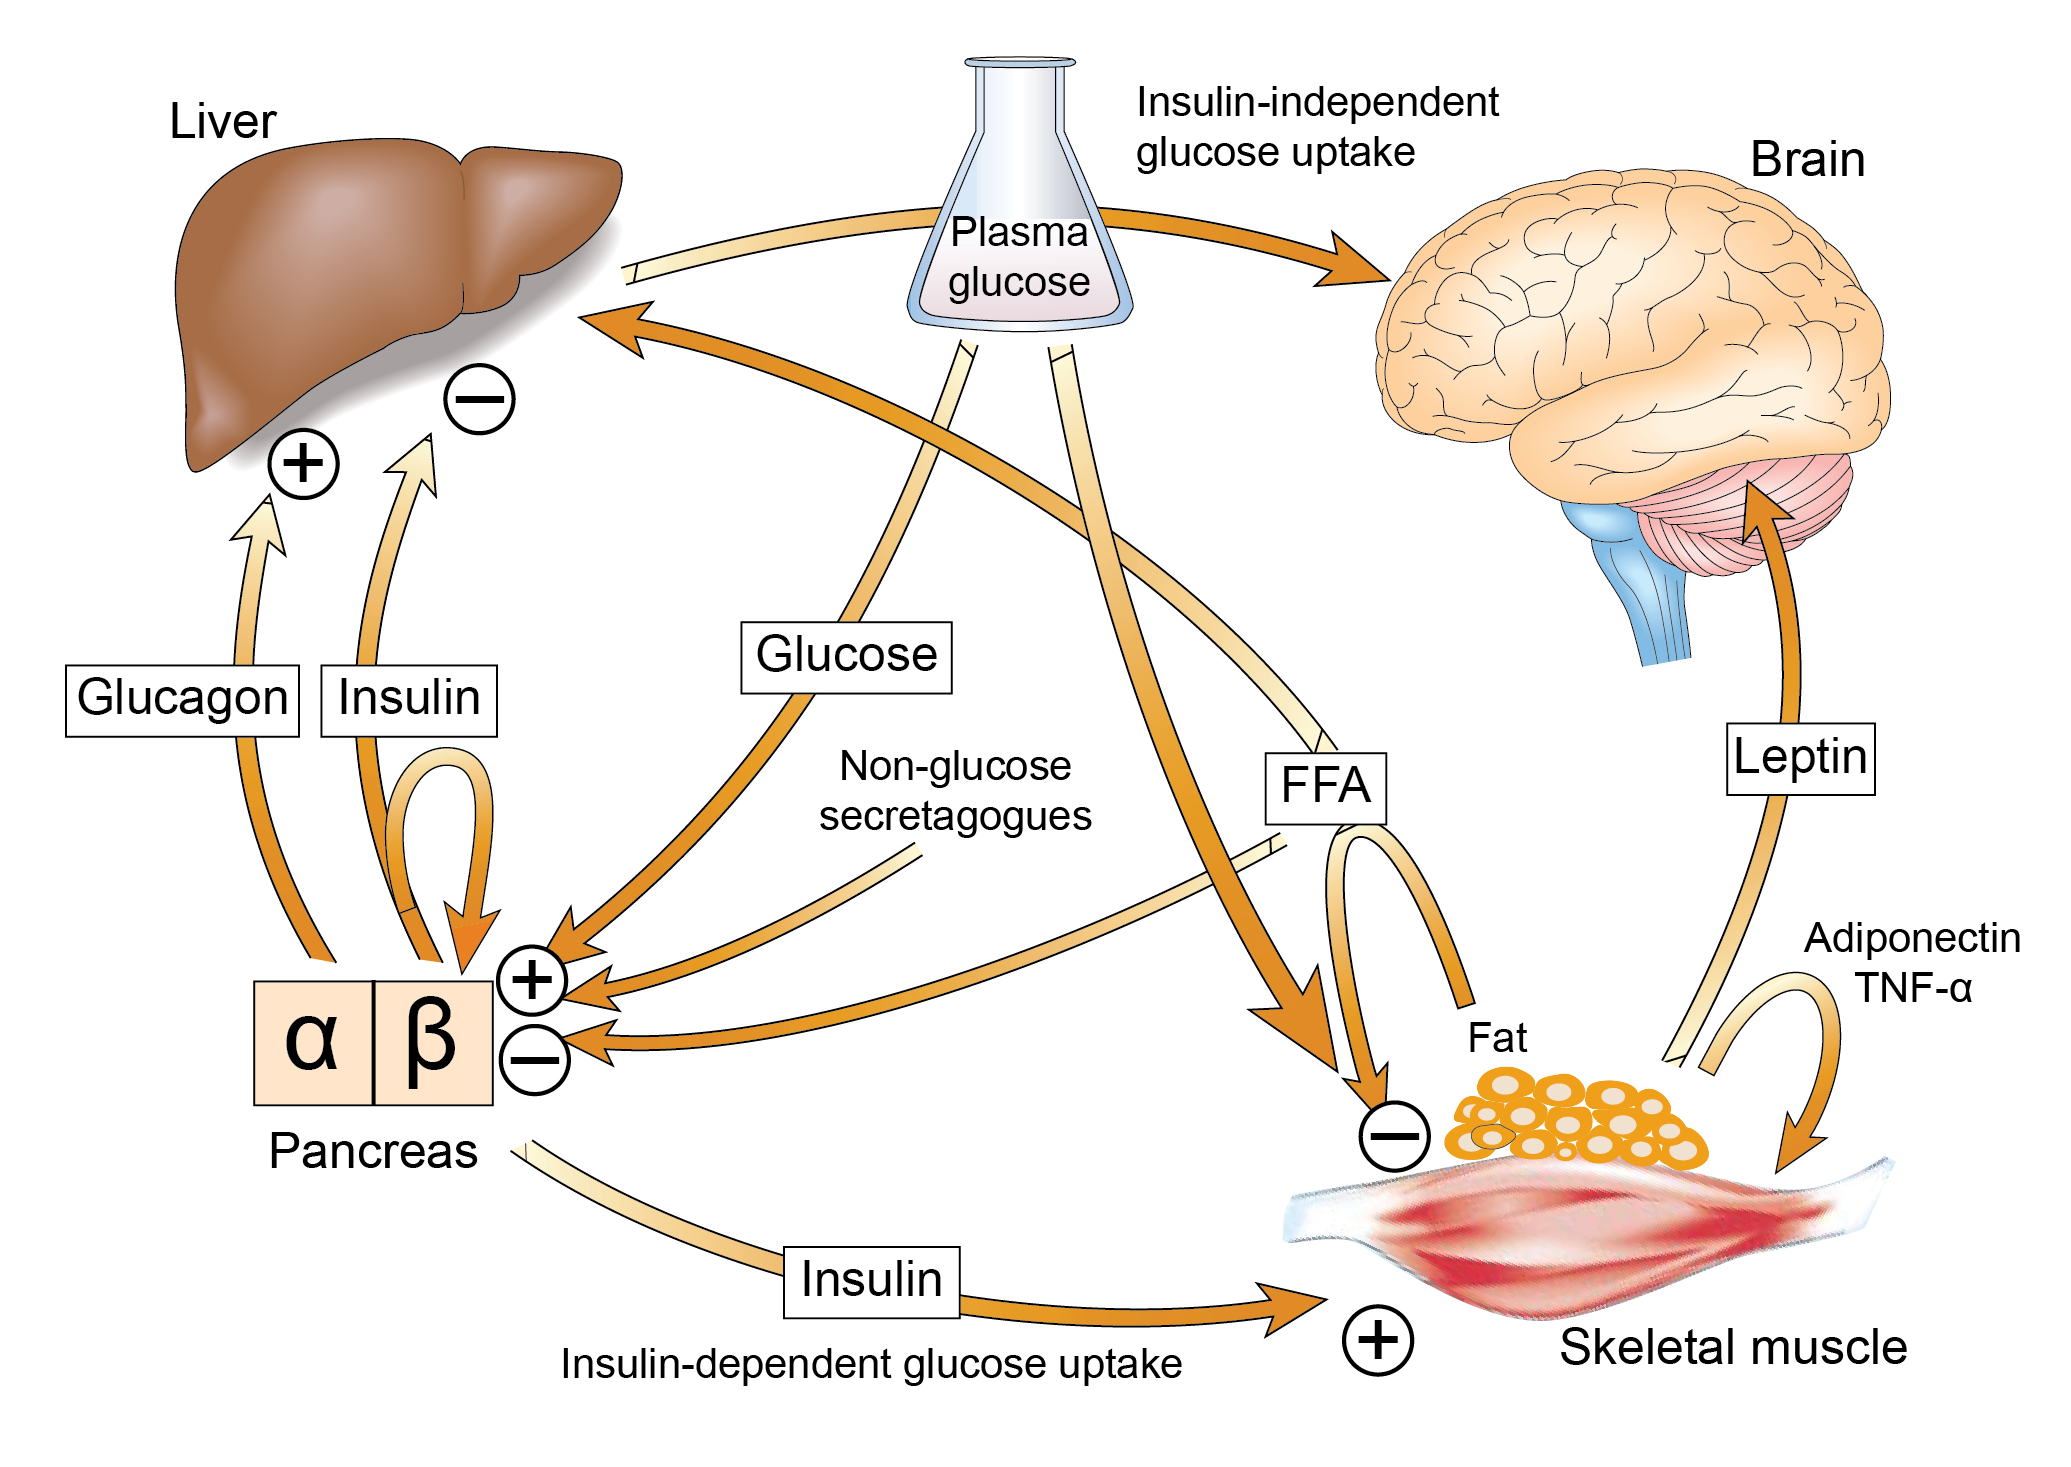
\includegraphics[width=\linewidth]{Chapter1/Fig/F1-13-01.png}
%     \caption{Caption}
%     \label{fig:enter-label}
% \end{figure}

% \begin{wrapfigure}{r}{0.5\textwidth}
%     \centering
%     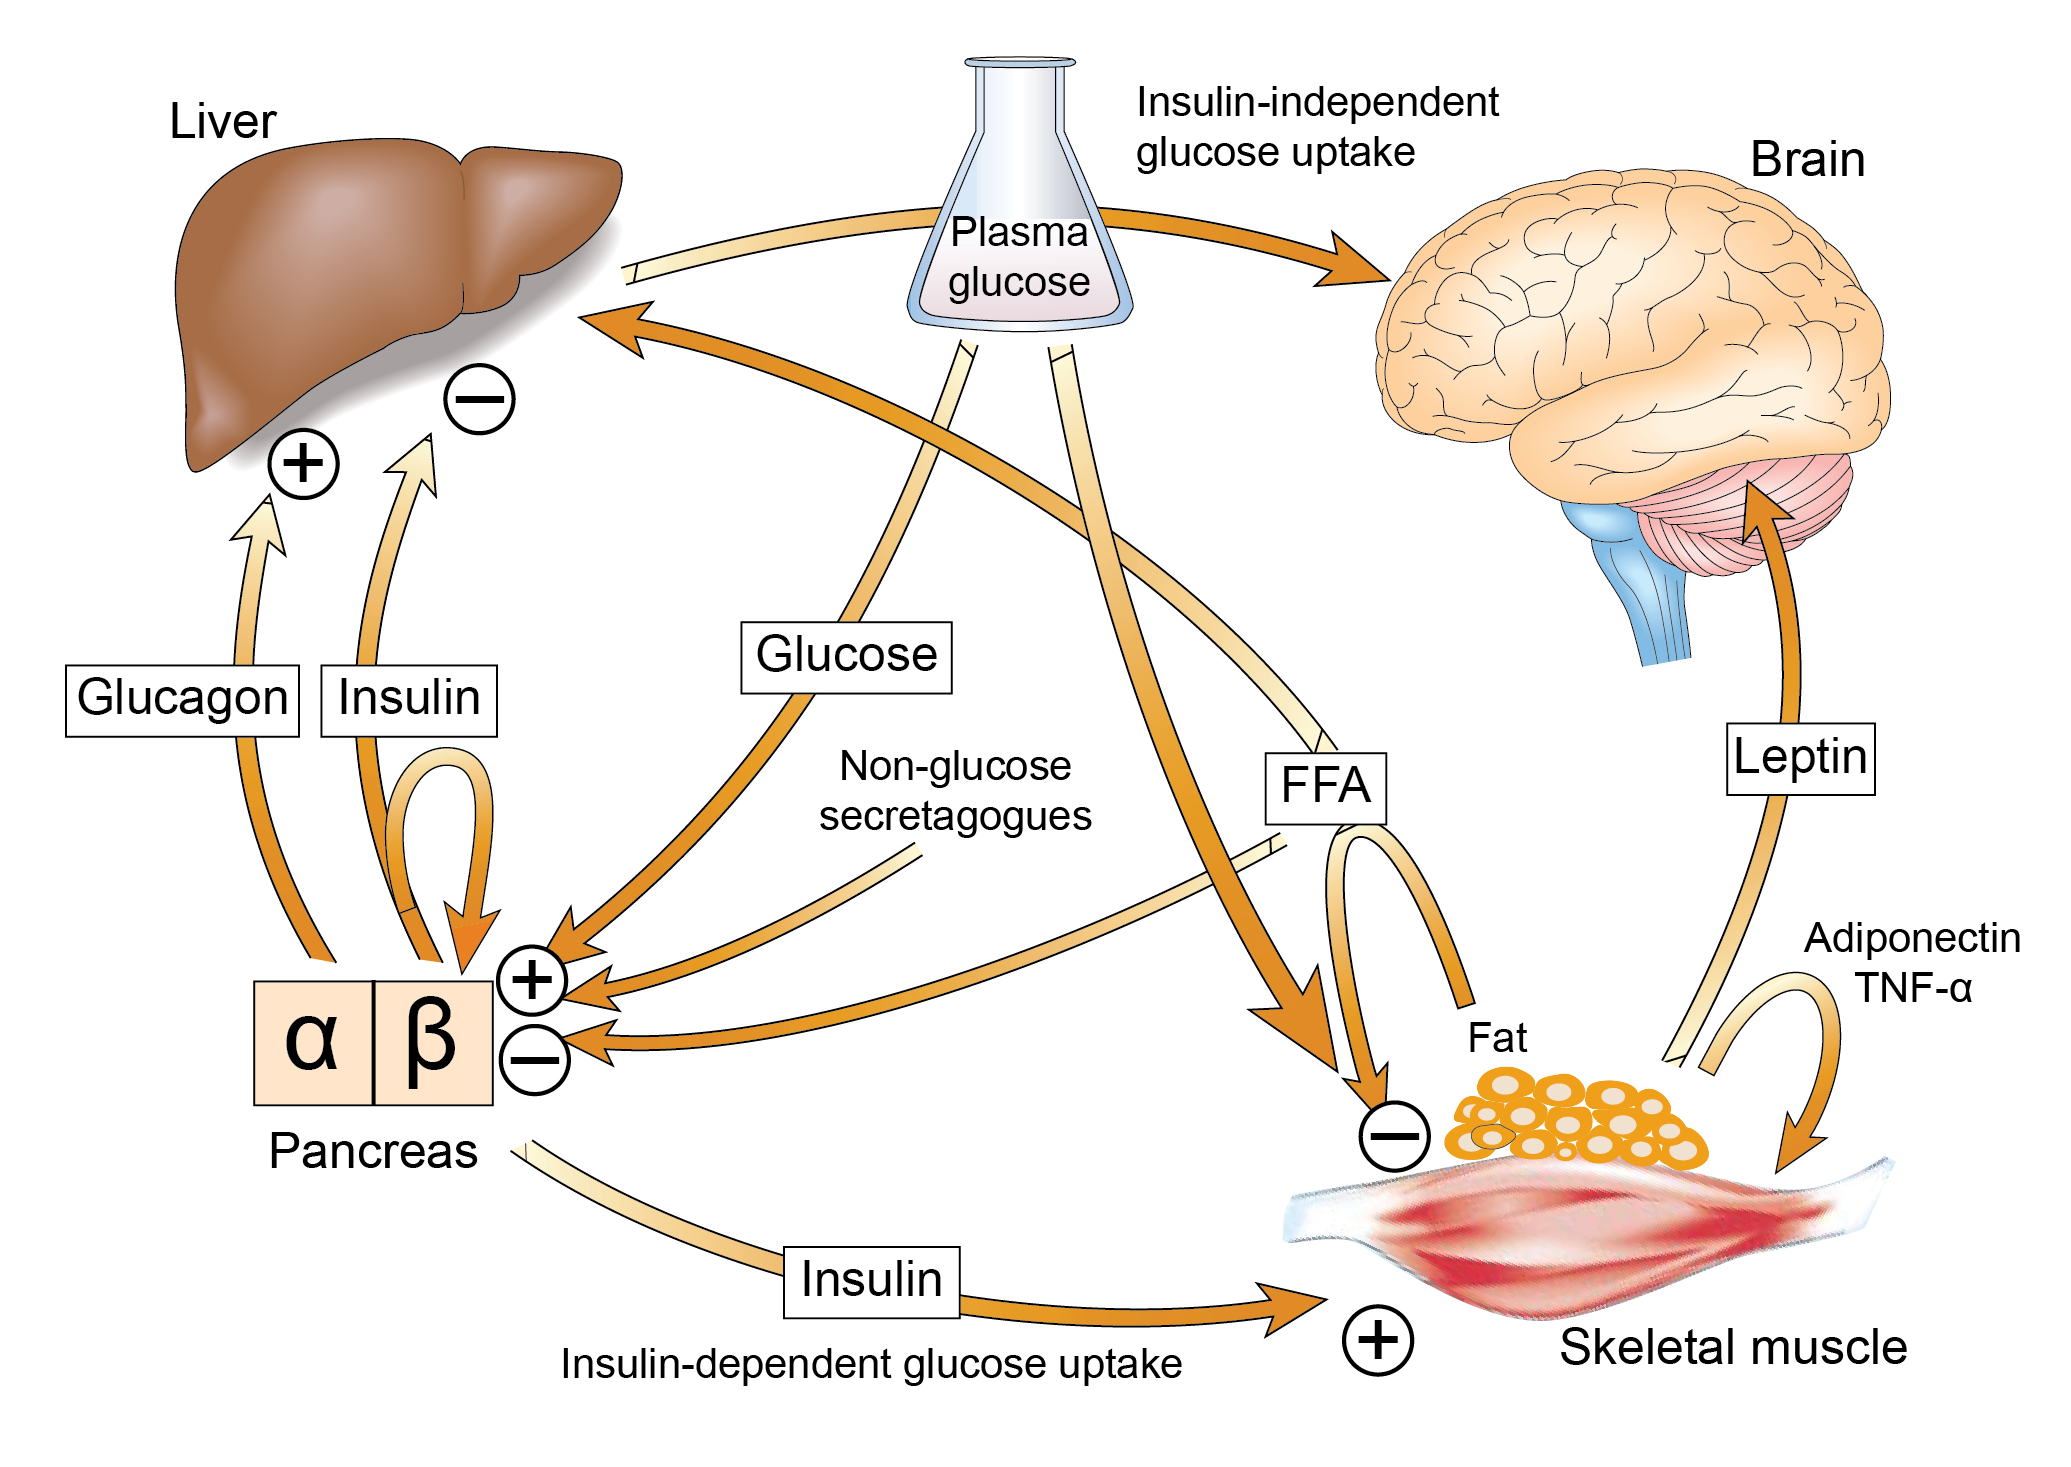
\includegraphics[width=8cm]{Chapter1/Fig/F1-13-01.png}
%     \caption[]{}
%     \label{fig:chp1_ins_action}
% \end{wrapfigure}

% \subsubsection{Liver}
% %The liver is exposed to higher insulin concentrations as insulin from pancreas is secreted into portal vein \textbf{\cite{petersen_mechanisms_2018}}. 
%  %The hepatic insulin signaling cascade upregulates several genes involved in \textit{de novo} lipogenesis thereby promoting lipid storage in hepatocytes and reduced export of very-low-density lipoprotein (VLDL) \textbf{\cite{petersen_mechanisms_2018,leavens_insulin_2011}} and reducing the availability of FA’s for oxidation by other tissues \textbf{\cite{petersen_mechanisms_2018,dimitriadis_insulin_2011}}. Insulin also mediates protein synthesis in hepatocytes via the mTOR network \textbf{\cite{petersen_mechanisms_2018,ROS}}.

% \subsubsection{Skeletal Muscles}
% Muscle  \st{and its subsequent conversion to glycogen via glycogen synthase (GS)} \st{leads to an increased concentration of glucose-6-phosphate (G6P), an allosteric activator of GS. Insulin also dephosphorylates and activates GS, which is further sensitized by G6P} Similar to glucose uptake via GLUT4, insulin stimulates translocation of several long-chain fatty acid transporters (CD36, FATP1/4) to cell membrane for the uptake of hydrophobic fatty acids and their subsequent metabolic processing and storage \textbf{\cite{sylow_many_2021,luiken_insulin_2002,wu_fatp1_2006,abumrad_membrane_1999}}. Insulin also stimulates amino acid uptake via amino acid transporters LAT1 and SNAT2 \textbf{\cite{sylow_many_2021,drummond_increase_2010}}, promotes subsequent protein synthesis, and curbs skeletal muscle protein breakdown \textbf{\cite{dimitriadis_insulin_2011,sylow_many_2021}}.

%\subsubsection{White Adipose Tissues (WAT)}


%\clearpage


%Insulin clearance is a crucial process in maintaining the homeostatic level of insulin required to reach the target tissues. The liver is plays a significant role in the clearance of the endogenously secreted hormone, accounting for up to 80\% of insulin degradation, during the first passage through the tissue \textbf{\cite{najjar_hepatic_2019,zaharia_reduced_2023}}. Thus, the liver regulates the flow of insulin into the systemic circulation and insulin action, thereby acting as a gatekeeper \textbf{\cite{cherrington_direct_1998}}. After the first passage, the insulin that is not degraded exits through the hepatic vein and reaches the heart, wherein it is pumped into arterial circulation and delivered to target tissues \textbf{\cite{tokarz_cell_2018}}. The circulating insulin is also subject to peripheral clearance by kidneys (via the glomerulus and proximal tubule) and other target tissues to a limited extent \textbf{\cite{najjar_hepatic_2019,polidori_hepatic_2016}}. After circulation, insulin returns to the liver and undergoes a second passage of clearance. The primary protease responsible for degrading insulin in tissues is known as insulin-degrading enzyme (IDE), and is ubiquitously expressed in tissues and has multiple cellular functions \textbf{\cite{duckworth_insulin_1998}}.  
Insulin-degrading enzyme (IDE) plays a major role in regulating the process of insulin clearance, is ubiquitously expressed in tissues and has multiple cellular functions \textbf{\cite{duckworth_insulin_1998}}. Up to 80\% of insulin degradation occurs in the liver through two separate passes, and additional peripheral clearance also occurs in the kidneys and other target tissues.


%\clearpage


% ********************************** % 1.2.7  **************************************
\subsection{Heterogeneity of $\beta$-cells} %Section - 1.2.7
\label{sec:beta_het}

% % %********************************** %Fourth Section  **************************************
% \section{\( \mathbf{\upbeta} \)-cell heterogeneity and adaptation in response to stress}

In any given multicellular biological system, cellular heterogeneity  can arise from developmental programs establishing cellular sub-types, from changes in cellular state due to altered environments or cell-intrinsic fluctuations, and from stochastic variation in gene expression. Cellular heterogeneity has been shown to be involved in development, adaptation to dynamic environmental conditions, repair and regeneration, as well as disease.
While it has long been apparent that not all $\beta$-cells in adult islets are identical, recent technological advances have shed further light on $\beta$-cell heterogeneity in terms of their morphology, identity and function. Although \gls{gsis} is the key function of mature $\beta$-cells, some $\beta$-cells may also retain non-secretory roles, necessary for overall islet function \textbf{\cite{liu_all_2017}}. This heterogeneity in $\beta$-cells is driven by topography and developmental origin \textbf{\cite{puri_plasticity_2015,roscioni_impact_2016}}, maturation state \textbf{\cite{salinno_-cell_2019}}, and stress response \textbf{\cite{xin_pseudotime_2018}}. Recent advances in characterization of $\beta$-cell heterogeneity have raised several important questions about the physiological significance of the prevalence of different $\beta$-cell sub-populations, their role in diabetes pathogenesis, and the plasticity of individual $\beta$-cells.

% \subsection{Previously established \( \mathbf{\upbeta} \)-cell heterogeneity}
% \colorbox{pink}{missing figure} \colorbox{green}{text clean-up} \colorbox{orange}{incomplete text} \\
\subsubsection{Historical Perspective}
In a study from 1960, Hellerström \textit{et. al.} identified regional differences in nuclear sizes and the position of nucleoli within the nuclei, depending on whether the $\beta$-cells were located centrally or peripherally in large or small islets in rat \textbf{\cite{hellerstrom_properties_1960}}. The authors further suggested that these cytological differences could be interpreted as corresponding differences in functional states of $\beta$-cells, as lower activity in centrally located $\beta$-cells in large islets could be due to cells being older or due to lower concentrations of glucose and/or insulin, compared to the cells in the periphery or in small islets \textbf{\cite{hellerstrom_properties_1960}}. In 1986, Salomon and Meda demonstrated that $\beta$-cells in rat islets were heterogeneous in their ability to release insulin \textbf{\cite{salomon_heterogeneity_1986}}. In particular, the group of Daniel G. Pipeleers carried out pioneering work in characterizing and describing $\beta$-cell heterogeneity in rodents: they identified distinct $\beta$-cell sub-populations differing in glucose responsiveness, insulin secretion and \glslink{nadph}{NADPH} levels \textbf{\cite{kiekens_differences_1992,schuit_glucose_1988,van_de_winkel_autofluorescence-activated_1983}}.\\

\subsubsection{Recent findings}
In the past years, several groups have identified additional markers of heterogeneity with $\beta$-cells that are less associated with the insulin secretory pathways. A recent study highlighted the role of Flattop (FLTP), a key element in the Wnt/planar cell polarity pathway, by using an islet-specific \textit{Fltp} reported mouse model \textbf{\cite{bader_identification_2016,roscioni_impact_2016}}. The authors showed clear and molecular physiological differences between FLTP\textsuperscript{+} and FLTP\textsuperscript{-} $\beta$-cells, with the FLTP\textsuperscript{+} $\beta$-cells making up \textasciitilde80\% of the $\beta$-cells in adult animals and exhibiting higher maturation and metabolic function. The authors also observed the expansion of both FLTP\textsuperscript{+} and FLTP\textsuperscript{-} populations , albeit to different stimuli \textbf{\cite{bader_identification_2016}}. In another study, Dorrell \textit{et. al.} identified four antigenically distinct subsets of $\beta$-cells based on differential expression of CD9 and ST8SIA1 in healthy human islets \textbf{\cite{dorrell_human_2016}}. Bulk RNA-sequencing analysis indicated diverse gene expression profiles and insulin secretion assays on the purified and reaggregated $\beta$-cell subsets revealed differential \gls{gsis}. Interestingly, the distribution of $\beta$-cell subsets was altered in the islets of patients with \gls{t2d} \textbf{\cite{dorrell_human_2016}}. A third study identified a small subset of $\beta$-cells termed hub cells within mouse islets, which were highly connected and exhibited distinct electrochemical characteristics, playing a crucial role in synchronizing Ca\textsuperscript{2+} signaling and insulin secretion across the islet \textbf{\cite{johnston_beta_2016}}. These hub cells, comprising 1\%-10\% of the $\beta$-cell population, showed enhanced and prolonged Ca\textsuperscript{2+} responses to glucose and were pivotal for maintaining synchronized signaling dynamics; disrupting these cells led to a significant decrease in synchronized activity and insulin-related zinc secretion \textbf{\cite{johnston_beta_2016}}. Despite their critical functional role, hub cells displayed a slightly undifferentiated phenotype with lower expression of key $\beta$-cell \glspl{tf} and reduced insulin production \textbf{\cite{johnston_beta_2016}}, highlighting a unique cellular mechanism within islet architecture that significantly influences overall islet function.\\
\par Building on the above recent studies about functional heterogeneity amongst $\beta$-cells, the advent of single-cell transcriptomics has provided researchers with the tools to investigate molecular heterogeneity at a much finer resolution and to subsequently connect these findings.

%\hl{FLTP, CD9 & Electrical coupling studies}

\subsubsection{$\beta$-cell diversity: Insights from \acrfull{scr}}
The field of single-cell biology has revolutionized the characterization of cells and led to the identification of novel cell-types, cell states and a better understanding of mechanisms in health and diseases. The topic of single-cell transcriptomics has been discussed in detail in \textbf{\autoref{sec:scrna}}. In the next paragraphs I highlight a few of the most recent single-cell studies that have investigated $\beta$-cell heterogeneity.\\\\ 
Single-cell analyses have recapitulated the previously described idea concept of functional $\beta$-cell heterogeneity and provided important new insights into $\beta$-cell biology. A study identified that mature and immature and/or proliferative $\beta$-cells co-exist in healthy mouse islets \textbf{\cite{sachs_targeted_2020}}. The immature $\beta$-cell cluster was characterized by down-regulation of genes involved in insulin secretion, oxidative phosphorylation and cell-cycle inhibition, as well as up-regulation of genes involved in \glslink{camp}{cAMP} and WNT signaling. Further, trajectory inference %(see \hyperref[sec:sc_tpi]{TI methods}) 
suggested a continuum of transition between the immature and mature states, rather than discrete phenotypes \textbf{\cite{sachs_targeted_2020}}. In another study employing mouse models, the authors defined $\beta$-cell maturity using arbitrarily defined levels of \textit{Pdx1} and \textit{Mafa}, and showed that adult islets are composed of mature (\textit{Pdx1}\textsuperscript{\textit{high}} \textit{Mafa}\textsuperscript{\textit{high}}) and immature (\textit{Pdx1}\textsuperscript{\textit{low}} \textit{Mafa}\textsuperscript{\textit{low}}) $\beta$-cells and the balanced proportion of these sub-populations might contribute to proper islet function and insulin release \textbf{\cite{nasteska_pdx1low_2021}}. Another study demonstrated the adaptive plasticity of $\beta$-cells to reversible chronic \glslink{er}{ER}-stress wherein $\beta$-cells undergo a reprogramming of their transcriptome and proteome \textbf{\cite{chen_adaptation_2022}}. More than half of the genes involved in \glslink{er}{ER} protein processing as well as markers of $\beta$-cell identity were compromised due to chronic stress whereas upon alleviation, $\beta$-cells regained their mature identity. The authors postulated that the heterogeneity in the maturity of $\beta$-cells in the islets might be a physiological response to cycles of \glslink{er}{ER}-stress and recovery \textit{in vivo} \textbf{\cite{chen_adaptation_2022}}.\\\\
With recent advances in the throughput of single-cell experiments, accumulating single-cell data and multiple analysis and integration approaches, large reference atlases comprising of millions of cells across several tissues, organs, developmental stages and/or conditions are now routinely generated \textbf{\cite{regev_human_nodate}}. These atlases help understand cellular heterogeneity, and provide an opportunity to learn from several single-cell datasets simultaneously, allowing for automatic annotation of new datasets and comparative analyses across several conditions \textbf{\cite{rood_impact_2022,lotfollahi_mapping_2021}}. The integrated \gls{mia} by Hrovatin \textit{et. al.} represents a comprehensive single-cell atlas of mouse pancreatic islets, integrating over 300,000 cells across multiple developmental stages and disease conditions \textbf{\cite{hrovatin_delineating_2023}}. The study also provided insights into the heterogeneity and dynamic states of $\beta$-cells during development, aging, and under diabetic conditions, depicted heterogeneous expression of known $\beta$-cell maturity and dysfunction markers across $\beta$-cell states and described pathways indicative of the different $\beta$-cell dysfunction phenotypes \textbf{\cite{hrovatin_delineating_2023}}. Overall, the \gls{mia} complemented the growing body of research on islet $\beta$-cell biology and highlighted the critical role of high resolution single-cell atlases.

%\clearpage

\subsection{$\beta$-cell adaptation and response to stress}
\colorbox{pink}{missing figure} \\

The production, storage and release of insulin by $\beta$-cells is tightly regulated in response to changes in metabolic status. The pathogenesis of \gls{t2d} is intricately linked to the dynamic response of $\beta$-cells to insulin resistance, wherein increased insulin demand is met by compensatory increases of insulin release, in order to maintain blood glucose homeostasis. %This ability to increase insulin production and secretion in response to hyperglycemia is a critical facet of $\beta$-cell function. 
Models that exhibit insulin resistant states while remaining normoglycemic provide excellent opportunity to study such $\beta$-cell compensation mechanisms \textbf{\cite{prentki_islet_2006, liu_beta-cell_2002}}. A zucker fatty (ZF) rat model showed the up-regulation of glucose-metabolism pathway with increased total glucose utilization and oxidation which likely contribute to compensatory hyperinsulinemia by increasing the activity of signaling pathways in \gls{gsis} \textbf{\cite{liu_beta-cell_2002}}. Similar compensatory responses of augmented insulin secretion have been reported in obese, non-diabetic patients and individuals with prediabetes \textbf{\cite{hudish__2019,chandrashekar_25-hydroxy_2015,polonsky_twenty-four-hour_1988}}. Furthermore, anaplerosis/cataplerosis pathways, signaling by \glspl{ffa}, increased sensitivity to incretin hormones as well as increased parasympathetic nervous system activity in the islets have all been implicated in compensatory $\beta$-cell responses \textbf{\cite{prentki_islet_2006}}. In addition to enhanced function, another well-studied feature of $\beta$-cell adaptation is $\beta$-cell proliferation to bring about changes in $\beta$-cell mass \textbf{\cite{hudish__2019}}.\\

\par However the up-regulation of \gls{gsis} in response to the constant and fast-changing demands of insulin pose unique challenges to $\beta$-cells. Compensation by $\beta$-cells require an accompanying increase in insulin biosynthesis, which can be regulated at the transcriptional, translational and posttranslational levels \textbf{\cite{prentki_islet_2006}}. The increase in rates of insulin biosynthesis in $\beta$-cells is associated with \glslink{er}{ER} stress, owing to large amounts of protein entering the secretory pathway \textbf{\cite{yong_therapeutic_2021}}.
%In addition to increased physiological demand, perturbation of \glslink{er}{ER} homeostasis can be brought about by other pathological conditions such as reactive oxygen species, infections and inflammation \textbf{\cite{fonseca_endoplasmic_2011}}. 
Under such demanding conditions, misfolded insulin and other misfolded proteins accumulate in the \glslink{er}{ER} lumen of $\beta$-cells, which activates the \gls{upr} pathway within the \glslink{er}{ER} \textbf{\cite{miranda_pancreatic_2021}}. The adaptive response by \gls{upr} transducers (IRE1$\alpha$, PERK and ATF6)  in $\beta$-cells establishes a return to cellular homeostasis and has been well-documented by studies in mouse models as well as in human patients with specific mutations, such as those with monogenic diabetes \textbf{\cite{yong_therapeutic_2021}}. The induction of \gls{upr} also up-regulates the \glslink{er}{ER}-associated protein degradation machinery (ERAD) that plays a crucial role for the maintenance of optimal $\beta$-cell function \textbf{\cite{yong_therapeutic_2021}}. A recent single cell analysis showed that healthy $\beta$-cells constantly undergo cycles of high and low \gls{upr} signaling, highlighting the importance of \gls{upr} dynamics in normal $\beta$-cell physiology \textbf{\cite{xin_pseudotime_2018}}.\\

%\clearpage

\par Chronic periods of increased insulin demand caused by a combination of multiple factors including peripheral insulin resistance \textbf{\cite{petersen_mechanisms_2018}}, nutrient-induced metabolic stress \textbf{\cite{prentki_nutrient-induced_2020,cnop_endoplasmic_2017}} and inflammatory mediators \textbf{\cite{eizirik_pancreatic_2020,cosentino_crosstalk_2021}}, eventually results in $\beta$-cell dysfunction. The $\beta$-cell dysfunction is characterized by perturbation of \glslink{er}{ER} homeostasis and maladaptive \gls{upr} responses \textbf{\cite{kalwat_pancreatic_2021}}. A central component of $\beta$-cell dysfunction in the pathogenesis of \gls{t2d} is the loss of functional mature identity, termed as dedifferentiation \textbf{\cite{miranda_pancreatic_2021}}. This was demonstrated in a single-cell study of non-diabetic and \gls{t2d} adults, wherein the $\beta$-cell gene signatures of adult \gls{t2d} samples were less well-defined compared to non-diabetic adults \textbf{\cite{wang_single-cell_2016}}. This dedifferentiation has also been recapitulated by mouse models of hyperglycemia \textbf{\cite{sachs_targeted_2020,oppenlander_vertical_2021}}. Dedifferentiated $\beta$-cells have expression of developmental genes, low expression of genes associated with mature $\beta$-cells including \textit{Pdx1, Mafa, Foxo1} and \textit{insulin}, and low \gls{gsis} \textbf{\cite{miranda_pancreatic_2021}}. The exact mechanisms for the loss of $\beta$-cell identity remain elusive and are a subject of active research especially in the context of exploring therapies or treatments that target the redifferentiation of the dedifferentiated $\beta$-cells as an intuitive way of treating diabetes. Few studies have reported on the partial reversal of the dedifferentiated $\beta$-cell state by strict dietary intervetion \textbf{\cite{sheng_reversibility_2016,ishida_pair_2017}} and combined insulin and \glslink{glp1}{GLP-1}/estrogen conjugate-mediated targeted delivery to $\beta$-cells \textbf{\cite{sachs_targeted_2020,oppenlander_vertical_2021}}.\\

A comprehensive understanding of the longitudinal sequence of $\beta$-cell compensatory mechanisms transitioning to dedifferentiated states and ultimately $\beta$-cell failure is still unknown. Investigative focus on mouse models which present a predictable disease progression could provide an important avenue for delineating these events. In the \gls{mia}, Hrovatin \textit{et. al.} deciphered the relationship between healthy and diseased states by identifying a shared intermediate state prior to the \gls{t1d} or \gls{t2d} model state \textbf{\cite{hrovatin_delineating_2023}}. Further examination of this intermediate state revealed differences in expression of most of the shared diabetes \gls{de} genes between healthy and intermediate states and further changed in the diabetic states. Based on these observations, the authors concluded that the intermediate state could represent a snapshot of the progression of $\beta$-cell dysfunction during diabetes \textbf{\cite{hrovatin_delineating_2023}}. Furthermore, much earlier to $\beta$-cell dysfunction, short term (feeding) as well as chronic nutrient stimulation (obesity) are also associated with transcriptional changes in the islets that enable functional adaptations by $\beta$-cells to proportionally adjust nutrient-induced insulin secretion \textbf{\cite{wortham_nutrient_2023}}. Taken together, these observations possibly suggest the existence of an intermediate $\beta$-cell state likely characterized by initial functional adaptations in response to increased insulin demand, thereby showcasing remarkable compensatory plasticity. The inability of $\beta$-cells to sustain this adaptive response upon chronic and unresolvable stress contributes to a vicious cycle of \glslink{er}{ER} and oxidative stress, pro-inflammatory cascades and signaling dysregulation, all of which is likely detrimental to $\beta$-cell function and identity, thereby leading to $\beta$-cell failure.\\

% However, the failure of β-cells to compensate for insulin resistance results in overt diabetes



% The adaptation by $\beta$-cells to the constant and fast-changing demands of insulin production and secretion is associated with 

% Secretory cells like the pancreatic $\beta$-cells are more susceptible to \glslink{er}{ER} stress    


% It is evident from rodent studies that, both, expansion of $\beta$-cell mass and enhanced $\beta$-cell function are important for $\beta$-cell compensation. 


% . β-cell dysfunction is characterized by loss of identity and lack of function.\\\\
% A central component of β-cell dysfunction in \gls{t2d} is the loss of functional mature identity and return to a progenitor-like state, termed as `dedifferentiation'. The dedifferentiation process is attributed to several factors such as oxidative stress, gluco- and lipo-toxicity, pro-inflammatory cytokines and altered gene expression.\\
% In particular, using \gls{paga}, Hrovatin et. al \textbf{\cite{hrovatin_delineating_2023}} further deciphered the relationship between healthy and diseased states by identifying a shared intermediate state prior to the T1D or T2D model state. Further examination of this intermediate state revealed differences in expression of most of the shared diabetes DEGs between healthy and intermediate states and further changed in the diabetic states. Based on these observations, the authors concluded that the intermediate state could represent a snapshot of the progression of β-cell dysfunction during diabetes. 


%Based on clinical observations and work with animal models of diabetes, Weir \& Bonner-Weir proposed five stages of β-cell dysfunction during diabetes progression \textbf{\cite{weir_five_2004}}. The stages describe changes in β-cell mass, phenotype and function, ranging from initial compensation (Stage-1) with increased insulin secretion and intact β-cell function, through adaptation (Stage-2) and early decompensation (Stage-3) characterized by rising glucose levels and β-cell de-differentiation, to stable (Stage-4) and severe (Stage-5) decompensation marked by significant loss of β-cell mass and function. 


% Failure of β-cell compensation is the defining event during the progression of \gls{t2d}. 

\clearpage

% ***************************************************************
%************************ %fourth Section %****************************************************************
\section{Islet inflammation}  %Section - 1.4
\label{sec:inflammation}

% \begin{Abstract}
% \vspace{3mm}

% \vspace{3mm}
% \end{Abstract}
% \vspace{3mm}

\subsection{The immune system}

\par The immune system constantly protects any organism from (pathogenic) threat, and involves a complex, interconnected system of specialized organs, tissues, effector cells and molecules. Immune dysfunctions or immunodeficiencies can be linked to severe autoimmune disorders, increased risk of lethal infections or developing cancer. The immune system is separated into two parts based on their mechanisms of antigen recognition, the subsequent kinetics of immune response and the ability for memory formation: \textit{innate immunity}, which is evolutionarily conserved and \textit{adaptive immunity}, which has evolved in vertebrates such as humans and rodents \textbf{\cite{orange_natural_2013,murphy_janeways_2017}}.\\

% \begin{figure}[H]
%     \centering
%     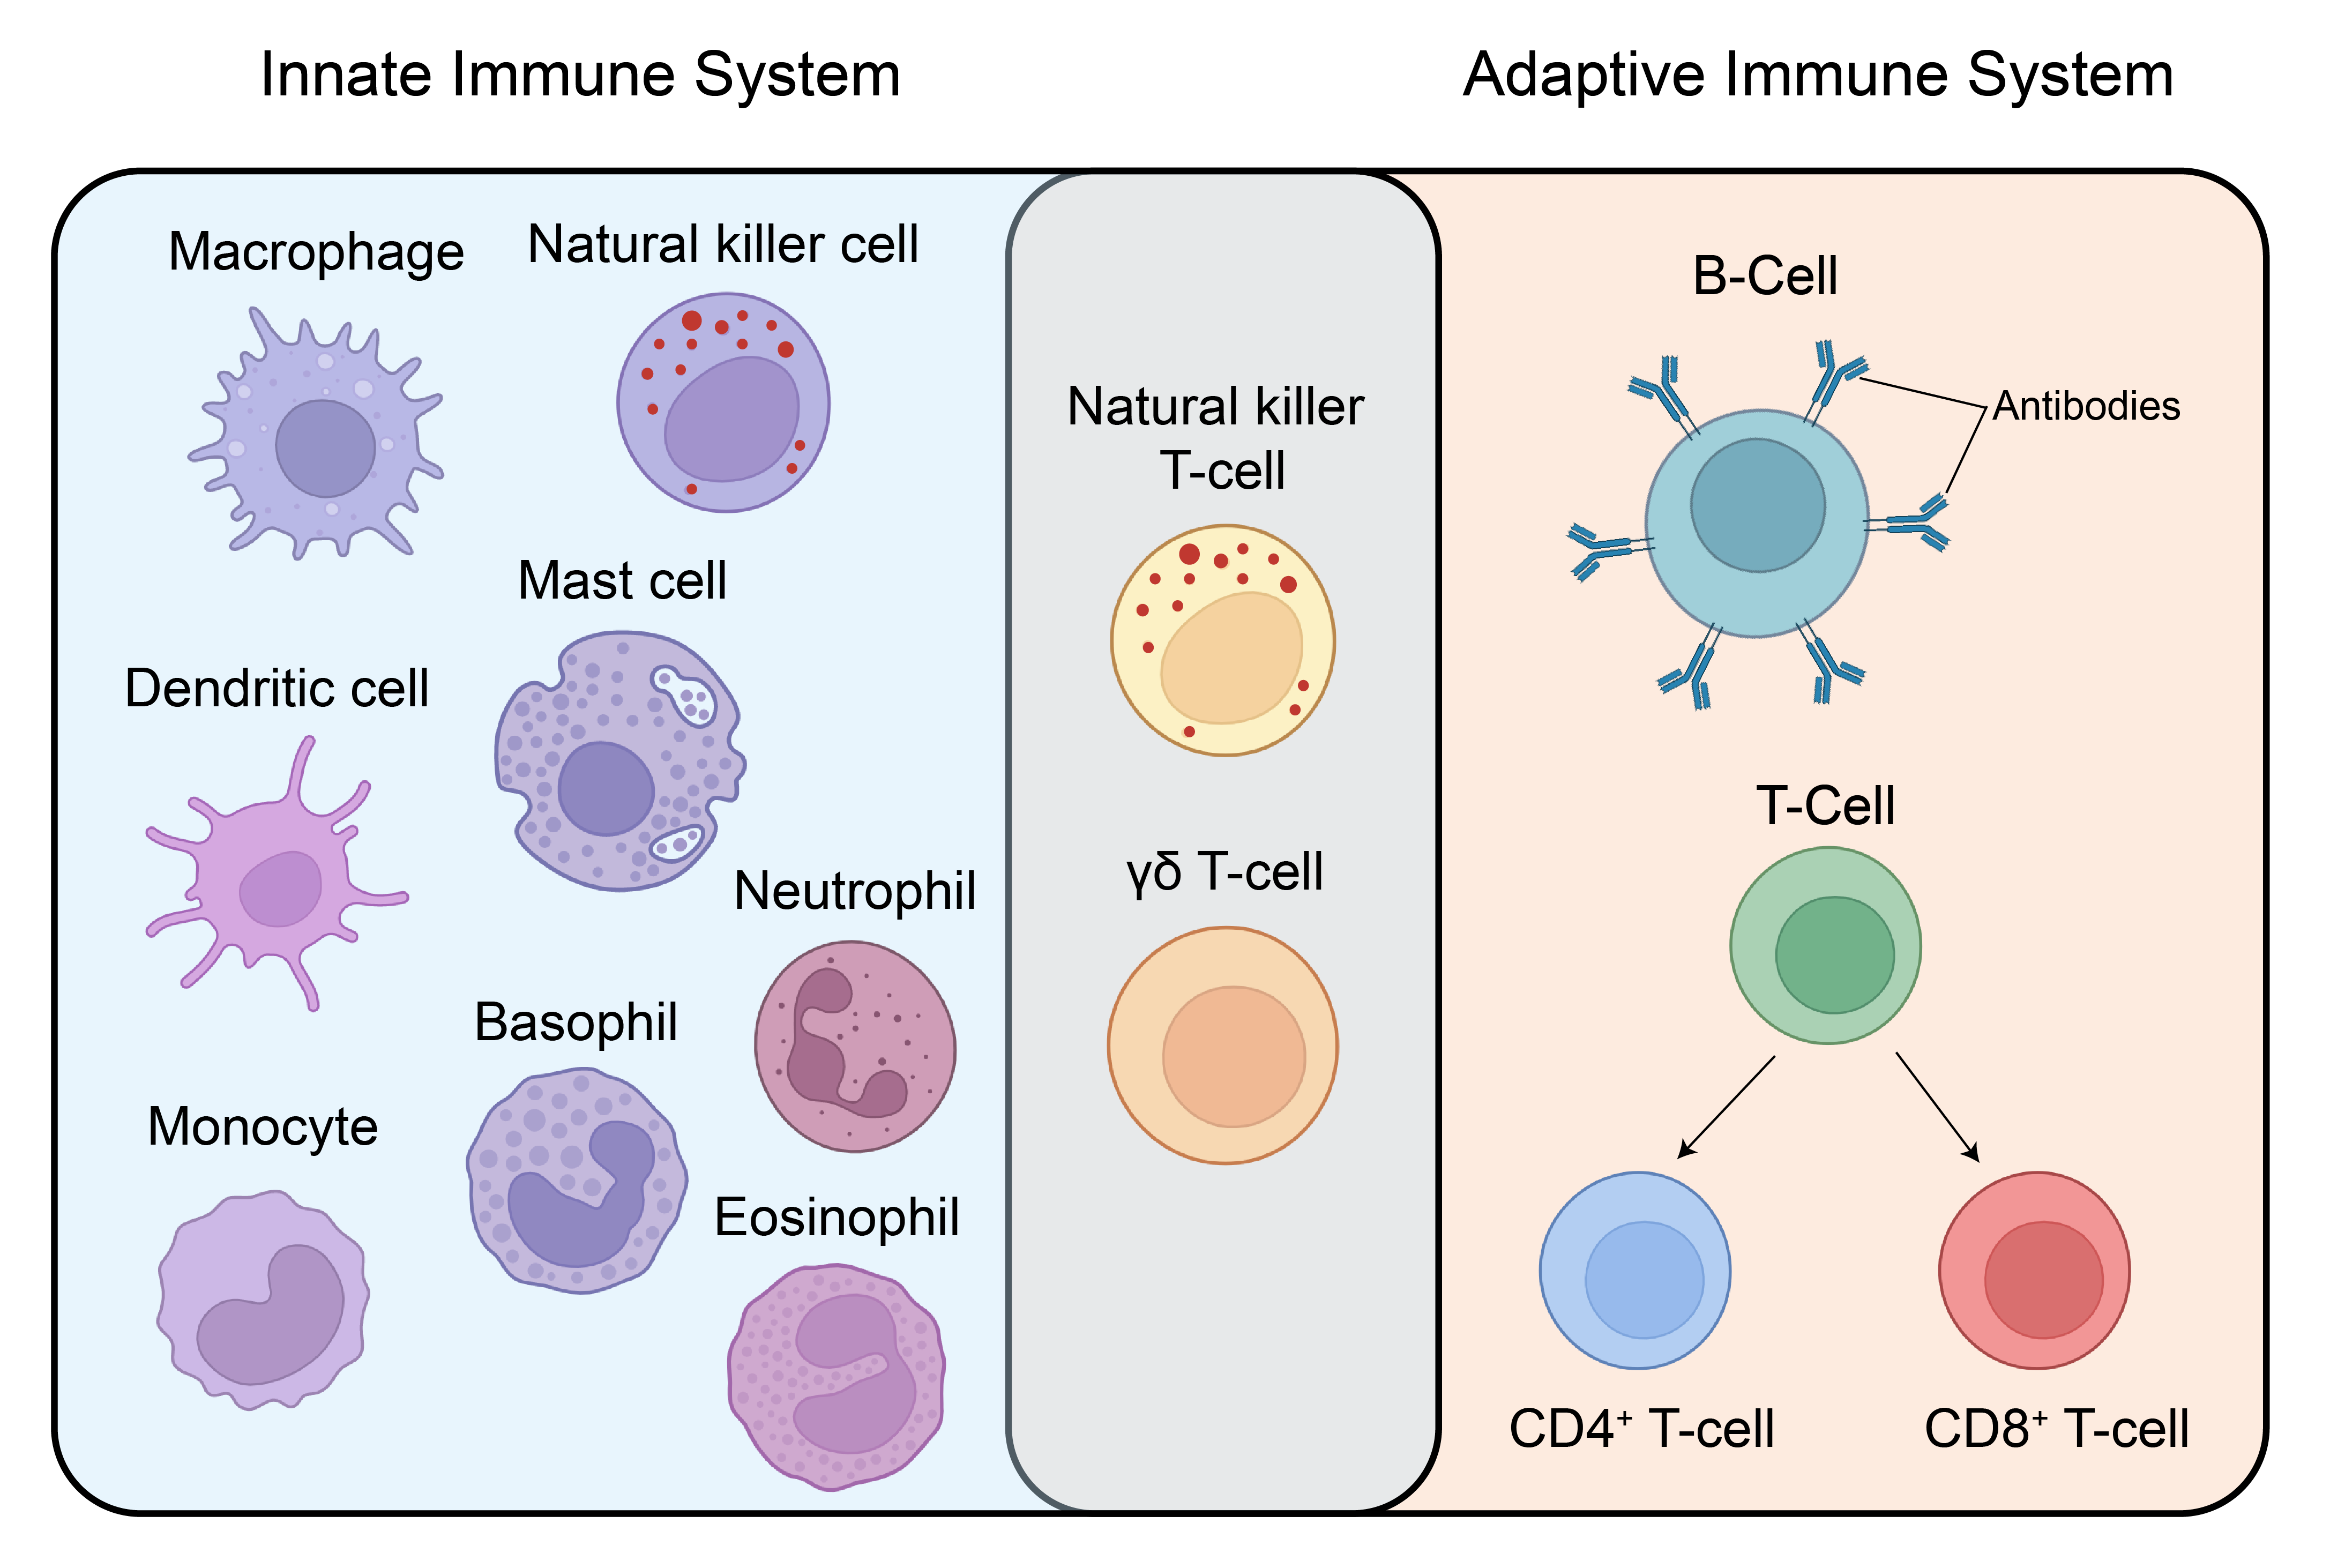
\includegraphics[width=10cm,height=8cm,keepaspectratio]{Chapter1/Fig/F1-15-01.png}
%     \caption[Overview of immune system]{}
%     \label{fig:chp1_immunesystem}
% \end{figure}

\begin{wrapfigure}{l}{0.5\textwidth}
    \centering
    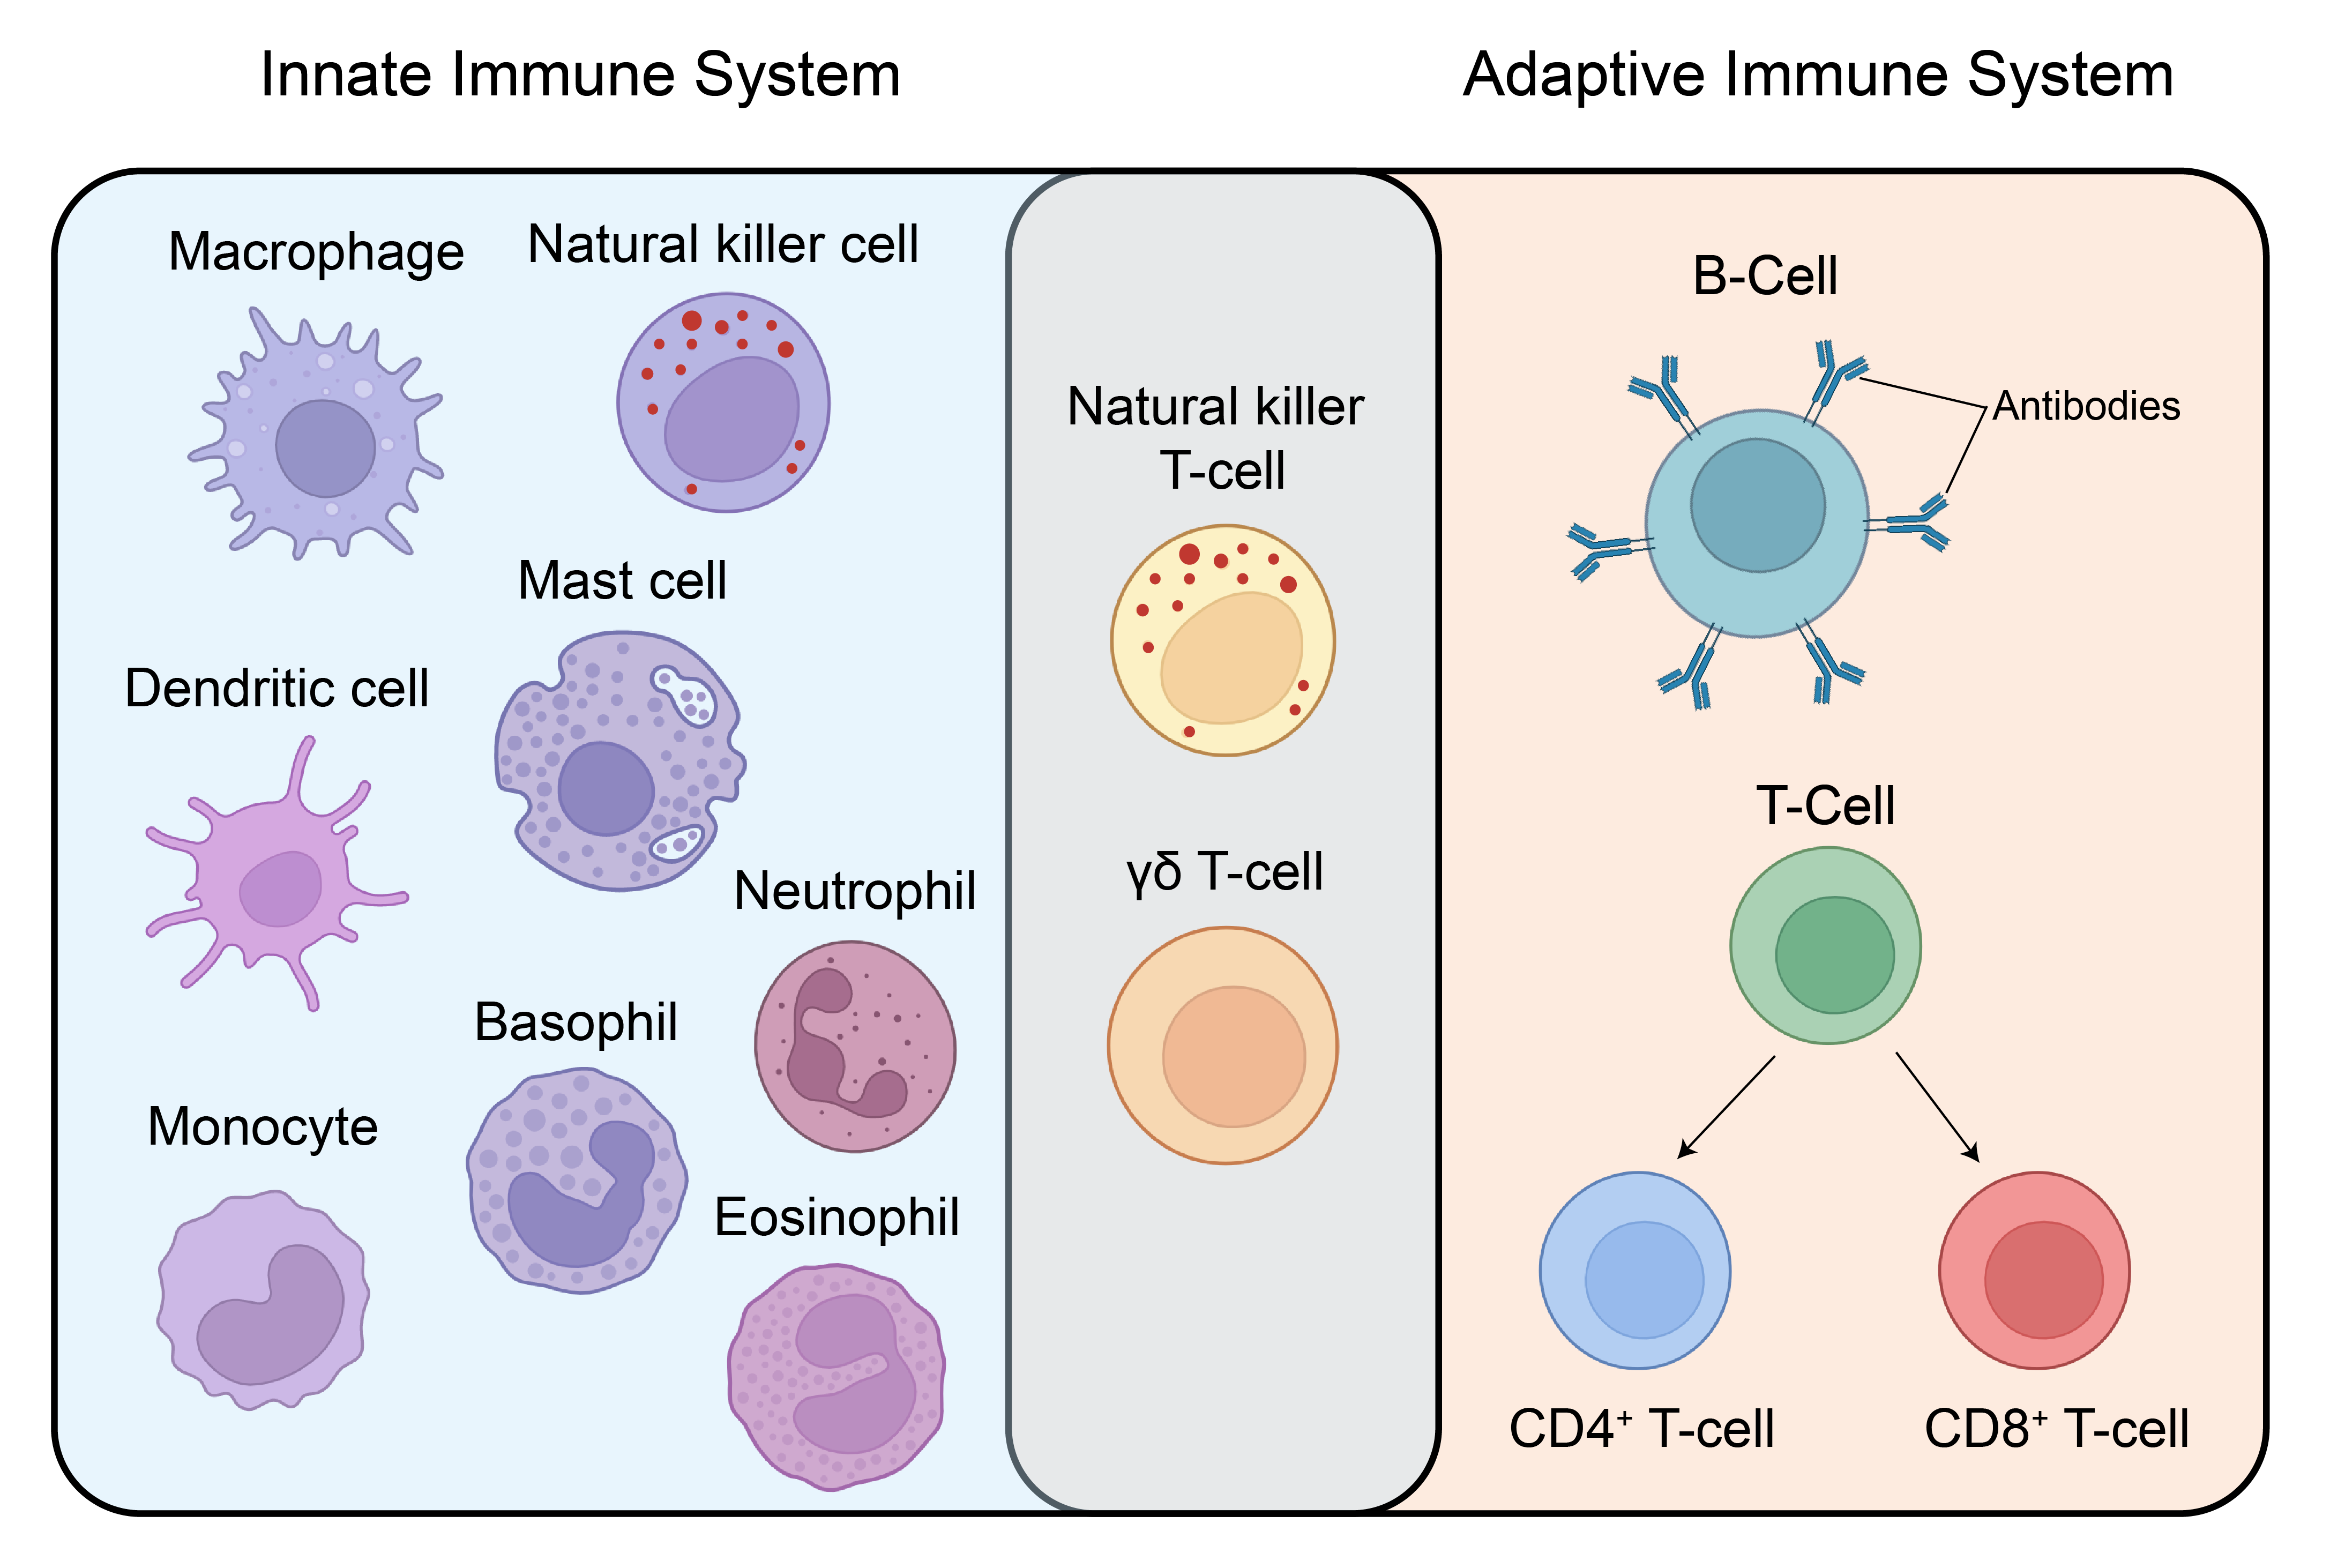
\includegraphics[width=7cm]{Chapter1/Fig/F1-15-01.png}
    \caption[Cells of the immune system]{\textbf{Cells of the innate and adaptive immune system.} The innate immune response forms the first line of defence against infections and consists of macrophages, dendritic cells, mast cells, monocytes, natural killer cells and granulocytes (neutrophils, basophils and eosinophils). The adaptive immune response is slow but highly specific and is capable to form immunological memory, and consists of B-cells and T-cells (CD4\textsuperscript{+} and CD8\textsuperscript{+}). Natural killer T-cells and $\gamma\delta$ T-cells function at the interface of the two immune responses. \textit{This figure is adapted from} \textbf{\cite{dranoff_cytokines_2004}}.\textit{ Reproduced with permission from Springer Nature}. Created with \href{https://www.biorender.com/}{Biorender.com}.}
    \label{fig:chp1_immunesystem}
\end{wrapfigure}

 \par The innate immune system is composed of anatomical barrier such as skin and chemical barriers such as the acidic environment in the stomach, and is characterized by a rapid response against variety of different pathogens. Innate immunity is mediated by humoral as well as cellular components which include phagocytic cells (Macrophages, Monocytes, Neutrophils and Dendritic cells), granulocytes (Basophils and Eosinophils), mast cells and \glspl{ilc} and Natural Killer cells (NKs). On the other hand, the adaptive immune system is characterized by a delayed but strong and antigen-specific immune response, with the capability to form immunological memory. The adaptive immune system is primarily composed of B-lymphocytes (B-cells) and T-lymphocytes (T-cells), each comprising of antigen-specific surface recep- \clearpage -tors, enabling response against wide variety of antigens \textbf{\cite{murphy_janeways_2017,chaplin_overview_2010,marshall_introduction_2018}}.

\subsection{Immune cells in the pancreas}
The immune landscape of the exocrine pancreatic tissue in mice is heterogeneous and consists of macrophages, monocytes, dendritic cells, B-cells. T-cells and \glspl{ilc} \textbf{\cite{calderon_pancreas_2015}}. This is summarized in \textbf{Table \ref{tab:chp1_immunecells}}. Most of the detailed analyses of tissue-resident macrophages in the pancreas have been carried out in mouse models. Macrophages are present in the pancreas from the embryonic state onwards. The pancreas in mice contains three sets of macrophages and their origins and phenotypes differ within the intrapancreatic microenvironment. Within the exocrine stroma, the macrophages were composed of two distinct sets that can be distinguished based on their embryological development and by the expression of the mannose receptor, CD206 and CD301 (\textit{Clec10a}) \textbf{\cite{calderon_pancreas_2015,cruz_macrophages_2020}}. CD206/CD301 low macrophages are constantly maintained from blood monocytes and are dispersed throughout the stroma, whereas CD206/CD301 high macrophages are derived from yolk-sac hematopoiesis, are enriched around pancreatic ducts and proliferate locally \textbf{\cite{calderon_pancreas_2015,cruz_macrophages_2020}}. The inter-acinar stromal macrophages are ten times more abundant than the islet macrophages.\\
\par In contrast to their counterparts in the exocrine tissue, islet-resident macrophages are of definite hematopoiesis origin, remain in the islets after birth, maintain modest levels of replication, and do not easily interchange with blood monocytes throughout steady state \textbf{\cite{calderon_pancreas_2015,cruz_macrophages_2020,carrero_resident_2017}}. However, a recent study identified two islet macrophage populations in mice: an intra-islet CD11c\textsuperscript{+} and a peri-islet CD11c\textsuperscript{-} cells, with the proportion of the CD11c\textsuperscript{+} subset being significantly increased after diet-induced obesity. Contrastingly, the abundance of the peri-islet CD11c\textsuperscript{-} population was not altered in response to a \gls{hfd} feeding \textbf{\cite{ying_expansion_2019}}. The islet macrophages are located next to intra-islet blood vessels are in close contact with $\beta$-cells. They constantly survey large areas of the islets and blood vessels through their filopedia. \textbf{\cite{carrero_resident_2017,calderon_dendritic_2008,zinselmeyer_resident_2018}}. Islet macrophages display an activated phenotype and express high levels of \gls{mhc2} and a number of cytokines and chemokines including TNF-$\alpha$ and IL-1$\beta$ \textbf{\cite{calderon_pancreas_2015,carrero_resident_2017,ferris_islet-resident_2017}} On average, there are 5-10 macrophages per mouse islet, and their number increases with islet size \textbf{\cite{unanue_macrophages_2016}}. Thus, compared to the exocrine macrophages, islet macrophages may hold distinctive functions that are specific to the islet niche.\\
%\clearpage
\par Evidence for the role of macrophages in the development of endocrine pancreas comes from the macrophage-deficient (\textit{Csf1\textsuperscript{op/op}}) mice which displyed major $\beta$-cell mass deficit, abnormal postnatal islet morphogenesis and impaired pancreatic cell proliferation \textbf{\cite{l_insulin_2004}}. Further, crosstalk between macrophages and epithelium drive the cell-cyle exit and migration of the embryonic pancreatic epithelium thereby promoting endocrine differentiation \textbf{\cite{mussar_macrophageepithelium_2014}}. It is also likely that macrophages play a role in adult pancreatic regeneration with accumulating evidence depicting macrophage crosstalk with resident cells to promote $\beta$-cell proliferation and pancreas regeneration \textbf{\cite{cruz_macrophages_2020}}. Macrophages also take part in vascular remodeling during development thereby likely contributing, at least partially to $\beta$-cell development \textbf{\cite{van_gassen_concise_2015}} and during islet compensation \textbf{\cite{chittezhath_islet_2019}}. Macrophages appear to be necessary to reconstitute $\beta$-cell proliferation in a mouse model of $\beta$-cell specific overexpression of vascular endothelial growth factor-A (VEGF-A) which induces major $\beta$-cell loss in adult islets \textbf{\cite{brissova_islet_2014}}. Macrophages have also been described to induce $\beta$-cell proliferation following $\beta$-cell death via the secretion of insulin-like growth factor 1 (IGF-1) \textbf{\cite{nackiewicz_islet_2020}}.\\ 

\begin{table}[t]
\centering
\caption{Summary of immune cells in pancreatic exocrine tissue.}
\label{tab:chp1_immunecells}
\begin{tabularx}{\textwidth}{XccccXc}
\toprule
\rowcolor{headerblue}
\textbf{Celltypes} & \textbf{F4/80} & \textbf{CD11b} & \textbf{CD11c} & \textbf{\gls{mhc2}} & \textbf{Markers\textsuperscript{*}} & \textbf{\% of CD45\textsuperscript{+}} \\
\midrule
Macrophages & \Large + & \Large + & \Large + & \Large +/- & \scriptsize CD206\textsuperscript{+/-} CD301\textsuperscript{+/-} & \large $\sim$40\% \\
\midrule
Monocytes & \Large - & \Large + & \Large +/- & \Large +/- & \scriptsize Ly6C\textsuperscript{+}, CX3CR1\textsuperscript{+} & \large $\sim$8\% \\
\midrule
\multirow{2}{*}{\makecell{Dendritic cells}} & \Large - & \Large + & \Large + & \Large + & \scriptsize Zbtb46\textsuperscript{+} &\large $\sim$7\% \\
\cline{2-7}
 & \Large - & \Large - & \Large + & \Large + & \scriptsize $\sim$45\% CD103\textsuperscript{+}, $\sim$75\% Zbtb46\textsuperscript{+} & \large $\sim$12\%  \\
\midrule
B-cells & \Large - & \Large - & \Large - & \Large + & \scriptsize CD19\textsuperscript{+}, B220\textsuperscript{+} & \large $\sim$12\% \\
\midrule
\multirow{2}{*}{\makecell{T-cells}} & \Large - & \Large - & \Large - & \Large - & \scriptsize CD4\textsuperscript{+} & \large $\sim$5\% \\
\cline{2-7}
 & \Large - & \Large - & \Large - & \Large - & \scriptsize CD8\textsuperscript{+} & \large $\sim$5\% \\
\midrule
\glspl{ilc} & \Large - & \Large - & \Large - & \Large - & \scriptsize CD4\textsuperscript{-}, CD8\textsuperscript{-}, IL-17R$\alpha$\textsuperscript{+} & \large $\sim$6\% \\
\bottomrule
\end{tabularx}
\vspace{0.1cm}
\RaggedRight{\footnotesize \\ +, present; -, absent.\\ \textit{This table is summarized from} \textbf{\cite{calderon_pancreas_2015}} \textit{and is adapted from} \textbf{\cite{nackiewicz_islet_2020}}}

% \RaggedRight{\footnotesize +, present; -, absent.}
% \RaggedRight{\footnotesize This table is summarized from \textbf{\cite{calderon_pancreas_2015}} and is adapted from \textbf{\cite{nackiewicz_islet_2020}}}

\end{table}

\par The physiological role of the islet macrophages is to maintain islet homeostasis with a truly symbiotic relationship with both $\beta$-cells and macrophages influencing each other \textbf{\cite{unanue_macrophages_2016}}. Ying \textit{et al.} found that depletion of macrophages in lean mice resulted in impaired \gls{gsis} \textbf{\cite{ying_expansion_2019}}. While the mechanisms underlying the benefecial impact of macrophages on $\beta$-cell secretion at steady state remains to be elucidate, an interesting study identified  that islet macrophages %also express functional purinergic receptors that allow them to 
detect $\beta$-cell secreted interstitial \glslink{atp}{ATP} via functional purinergic receptors and sense $\beta$-cell secretory activity \textbf{\cite{weitz_mouse_2018}}, thereby providing a feedback loop for insulin secretion regulation. \glslink{atp}{ATP} activates the purinergic receptors and induces calcium responses in macrophages, gene expression changes and increased motility \textbf{\cite{cosentino_crosstalk_2021}}. Additionally, vesicles of different composition, including beta-cell derived insulin granules, and blood-derived micro-particles have been found within the cell body of the islet macrophages \textbf{\cite{vomund_beta_2015,zinselmeyer_resident_2018}}. Altogether, islet macrophages are highly active and release proliferative signals and constantly analyse the composition of their microenvironment in order to sense the secretory activity of $\beta$-cells and to control tissue homeostasis.\\


\par Under steady state, adaptive immune cells (such as T-cells and B-cells) are primarily found in the exocrine tissue of the pancreas and not within the islets \textbf{\cite{calderon_pancreas_2015, ying_expansion_2019}}.


% 



% Thus, the anatomy of the pancreas conditions the origins and properties of resident macrophages \textbf{\cite{calderon_pancreas_2015, unanue_macrophages_2016}}. 



% \begin{table}[H]
% \renewcommand{\arraystretch}{1}
% \centering
% \caption{Summary of Leukocyte Subsets in Pancreatic Stroma}
% % \begin{tabular}{@{}p{0.2\linewidth}p{0.1\linewidth}p{0.4\linewidth}p{0.1\linewidth}@{}}
% \begin{tabularx}{\textwidth}{C C x C}
% \toprule
% \rowcolor{headerblue}
% \textbf{Primary marker} & \textbf{Secondary marker} & \textbf{\% of CD45\textsuperscript{+}} & \textbf{Cell-types} \\ 
% \midrule
% 1st Set:\\
% F4/80\textsuperscript{+} CD11b\textsuperscript{+} & CD11c\textsuperscript{+} &  \Large \textasciitilde40\% & Macrophages \\
% & & \scriptsize \raggedright{\textasciitilde60\% MHC-II\textsuperscript{+},40\% CX3CR1\textsuperscript{+}} & \\
% %& &  \raggedright{\scriptsize 40\% CX3CR1\textsuperscript{+},} & \\
% & & \scriptsize \raggedright{50\% CD206\textsuperscript{+} and CD301\textsuperscript{+}} & \\ 
% \midrule
% % } & \\
% % & & \scriptsize \raggedright{CD301\textsuperscript{+}} & \\ 
% % 2nd Set:\\
% % F4/80\textsuperscript{-} CD11b\textsuperscript{+} & Ly6C\textsuperscript{+} CX3CR1\textsuperscript{+} &  & Monocytes \\
% %  & CD11c\textsuperscript{+} MHC-II\textsuperscript{+} Zbtb46\textsuperscript{+}  & & Dendritic cells\\

% \multirow{2}{*}{\makecell{2nd Set:\\
% F4/80\textsuperscript{-} CD11b\textsuperscript{+}}} & Ly6C\textsuperscript{+} CX3CR1\textsuperscript{+} &  & Monocytes  \\
%      \cline{2-4}
%      & CD11c\textsuperscript{+} MHC-II\textsuperscript{+} Zbtb46\textsuperscript{+} &  & Dendritic cells \\
   
% \midrule

% \multirow{5}{*}{\makecell{3rd Set:\\
% F4/80\textsuperscript{-} CD11b\textsuperscript{-}}} & Ly6C\textsuperscript{+} CX3CR1\textsuperscript{+} &  & Monocytes  \\
% \cline{2-4}
% & CD11c\textsuperscript{+} MHC-II\textsuperscript{+} Zbtb46\textsuperscript{+} &  & Dendritic cells \\
% \cline{2-4}
% & CD11c\textsuperscript{+} MHC-II\textsuperscript{+} Zbtb46\textsuperscript{+} &  & Dendritic cells \\
% \cline{2-4}
% & CD11c\textsuperscript{+} MHC-II\textsuperscript{+} Zbtb46\textsuperscript{+} &  & Dendritic cells \\
% \cline{2-4}
% & CD3e\textsuperscript{-} IL-17R$\alpha$\textsuperscript{+} &  & ILCs \\


% % CD11c\textsuperscript{+} & 
% % \Large \textasciitilde40\%\\
% % \small \textasciitilde60\% MHC-II\textsuperscript{+},\\
% % \small 40\% CX3CR1\textsuperscript{+}\\
% % \small 50\% CD206\textsuperscript{+} and CD301\textsuperscript{+} & \Large Macrophages  \\



% \bottomrule


    
% \end{tabularx}
% \end{table}

\subsection{Inflammation}
\label{sec:immune_inflammation}

\par Inflammation is usually defined as a local response to tissue injury or infection \textbf{\cite{donath_islet_2008}}, and is - initiated upon the disruption of cellular and tissue homeostasis / conventionally viewed as the opposing state to tissue homeostasis \textbf{\cite{meizlish_tissue_2021}}. Inflammation can be classified as acute or chronic. An acute inflammatory response is characterized by invasion of leukocytes, mainly neutrophils, into the extravascular tissue and the production and release of several chemokines and cytokines, and in some case is accompanied by collateral functional and structural damage to host tissue. After a successful inflammatory response, a resolution and repair phase ensues. The failure of an acute response results in the persistence of inflammation, wherein the neutrophil infiltrate is replaced by monocytes / macrophages and lymphocytes such as T-cells. In case of insufficient combined effect of these cell-types, a long-term maladaptive phase results in a chronic inflammatory state resulting in further complications \textbf{\cite{medzhitov_origin_2008}}. 

\subsection{Obesity \& Inflammation}
\label{sec:immune_obesity}

Over-nutrition and lack of physical activity results in the development of obesity, characterized by excess adiposity. Metabolic syndrome, a cluster of diseases resulting from complications of obesity are exerting severe burden on public health care systems worldwide. The worldwide epidemic of obesity is associated with low-grade, chronic inflammation of metabolic (metainflammation) tissues such as \gls{wat}, liver, muscle and pancreatic islets and has led to increase in metabolic diseases. A growing body of evidence suggests that many of the co-morbidities of obesity including \gls{t2d}, cardiovascular and neurodegenerative diseases exhibit this inflammatory state.\\
\par In \gls{t2d}, inflammation has also been observed in the pancreatic islets \textbf{\cite{boni-schnetzler_islet_2019}}. Inflammation of the islets’ during obesity is associated with an increase in myeloid-lineage cells, including monocytes and macrophages \textbf{\cite{eguchi_islet_2017,ying_role_2019}}. An elevation in macrophage numbers within the islets has been documented in both \gls{hfd}-induced \textbf{\cite{ehses_increased_2007}} and genetically modified (\textit{db/db}) overnutrition models \textbf{\cite{cucak_accumulation_2014}}. The origin of these macrophages is currently an active area of research. It has been shown that saturated \glslink{fa}{FA}s in the circulation can initiate chemokine production in $\beta$-cells, which then recruits monocyte-derived macrophages to the islets \textbf{\cite{eguchi_saturated_2012}}. However, recent findings indicate that this recruitment predominantly affects the macrophages in the peri-islet region. In contrast, macrophages inside the islets, characterized by \textit{CD11c} expression and lower F4/80 levels, appear to locally expand in response to overnutrition \textbf{\cite{ying_expansion_2019}}. In addition, phenotypic characterization of the of islet-resident macrophages during obesity remain controversial. While a pro-inflammatory phenotype has been linked to macrophages in obese islets, a similar phenotype was also observed in macrophages within healthy islets, though the total number of these cells is smaller \textbf{\cite{cucak_accumulation_2014}}. Furthermore, whole transcriptome analysis of macrophages from the islets of lean and obese mice did not reveal typical pro- or anti-inflammatory profiles \textbf{\cite{ying_expansion_2019}}, indicating that the classical categorization strategy may not be applicable in this context. This ambiguity could also be attributed to the heterogeneity of islet-resident macrophages, where different sub-populations respond uniquely to overnutrition.\\
\par Chronic meta-inflammation across insulin-sensitive tissues such as \gls{wat}, liver and muscle play a pivotal role in the pathogenesis of metabolic dysfunctions associated with obesity \textbf{\cite{gregor_inflammatory_2011,hotamisligil_inflammation_2017}}. This systemic inflammation is marked by the infiltration and accumulation of pro-inflammatory macrophages, altered T-cell subsets and other immune cells, and elevated levels of pro-inflammatory cytokines like TNF-α, IL-6, and IL-1β and other chemokines that disrupt insulin signalling pathways. These cytokines can activate intracellular signalling molecules such as NF-$\kappa$B or JNK which can drive increased expression of inflammatory mediators. Additionally, excess dietary nutrients such as glucose or \glspl{ffa} can drive the activation of inflammsomes which can further induce cytokine production. Also, chronic metabolic stress can cause disruption of \glslink{er}{ER} homeostasis, increased production of \gls{ros} and reduced anti-oxidant defence mechanisms, thereby activating inflammatory signalling pathways and exacerbating local and systemic inflammation. This common immune response dysregulation leads to peripheral insulin resistance, which is regarded as a central feature in the development of metabolic disorders such as \gls{t2d} \textbf{\cite{greenberg_obesity_2006,wu_metabolic_2020,luo_inflammation_2020,kawai_adipose_2021,kim_metabolic_2021,rohm_inflammation_2022,wu_skeletal_nodate}}.

\subsection{Aging \& Inflammation}
\label{sec:immune_aging}

Aging is a complex process marked by the gradual functional decline of various tissues and organs. These altering processes serve as major risk determining factors for \gls{t2d} and other adult-onset disorders \textbf{\cite{sandovici_ageing_2016,tuduri_pancreatic_2022}}. Aging is also associated with a chronic, low-grade inflammation, termed as \textbf{inflammaging} \textbf{\cite{frasca_aging_2017,franceschi_inflamm-aging_2000}}. This chronic state of background inflammation is characterized by elevated levels of pro-inflammatory markers, and is distinct from acute inflammation, which can be a short-term, beneficial response to injury or infection. A crucial factor driving inflammation during aging is cellular senescence, which is a state of permanent cell-cycle arrest \textbf{\cite{ren_inflammatory_2009}}. Senescent cells accumulate with age and have an elaborate secretory profile, commonly referred to as the senescence-associated secretory phenotype (SASP) \textbf{\cite{gorgoulis_cellular_2019}}. The SASP, which frequently encompasses cytokines, chemokines and other growth factors, mediates its effects through, among other mechanisms, immune cell recruitment thereby promoting chronic inflammation \textbf{\cite{gorgoulis_cellular_2019}}. At the same time, the age-related decline in immune function, known as immunosenescence, renders immune cells unable to clear senescent cells, pathogens and inflammatory factors \textbf{\cite{sanada_source_2018}}. This dysregulation of immune responses further contributes to the chronic inflammatory state. Innate cells, especially macrophages have been in the center of the inflammaging theory for a long time. However, research in the past decade has made it apparent that T-cells might be the immune population most drastically affected by age, as both, CD8 and CD4 T-cells undergo significant re-modeling, including changes in cell populations and cell-intrinsic re-programming \textbf{\cite{shchukina_t_2023}}. Apart from senescence, other potential mechanisms also contribute to inflammaging such as genetic susceptibility, chronic overstimulation of immune cells, altered gut microbiome and increased intestinal permeability, increased adiposity, oxidative stress caused by dysfunctional mitochondria, or chronic infections \textbf{\cite{frasca_aging_2017,ferrucci_inflammageing_2018,frasca_inflammaging_2016}}.\\

\par The age associated progressive decline in accurate regulation of glucose homeostasis may gradually result in impaired glucose tolerance and \gls{t2d}. The impairment of insulin-secretion in an age-associated manner has been consistently demonstrated in rodents and humans \textbf{\cite{sandovici_ageing_2016,muzumdar_decrease_2004}}. Aging also leads to the accumulation of senescent $\beta$-cells in the pancreatic islets \textbf{\cite{tuduri_pancreatic_2022}}, which exhibit decreased function and increased susceptibility to apoptosis, thereby contributing to impaired insulin secretion. The most consistent observation across humans and mouse is that of the decline in proliferative capacity of aged $\beta$-cells, and studies have also reported age-related decline in peripheral insulin sensitivity \textbf{\cite{tuduri_pancreatic_2022}}. Inflammaging is also linked to the concept of metainflammation, and both conditions share similar molecular mechanisms \textbf{\cite{franceschi_inflammaging_2018,prattichizzo_inflammageing_2018}}. The elevated pro-inflammatory cytokines are associated with decreased insulin sensitivity and development of insulin resistance \textbf{\cite{rehman_mechanisms_2016}}, and meta-inflammation causes excess nutrients such as lipids, \glspl{ffa}, glucose and \gls{ros} to promote chronic, low-grade inflammation \textbf{\cite{frasca_aging_2017}}. In contrast to the well-documented kinetics of islet inflammation in obesity, the dynamics of islet inflammation in an age-dependent context are less understood. An age-dependent accumulation of TNF-$\alpha$ producing macrophages has been observed in zebrafish, contributing to a decline in $\beta$-cell proliferation capacity \textbf{\cite{janjuha_age-related_2018}}. Additionally, while T-cells are typically rare in the islets, their significant accumulation has been noted in aging mice \textbf{\cite{denroche_t_2021}}. The enrichment of T-cells in the islets is not usually observed under obesity conditions \textbf{\cite{eguchi_islet_2017}}, indicating that aging and obesity might trigger distinct inflammation profiles.\\

\par Inflammaing also has profound effects on other orangs in the body. In the liver, inflammatory mediators drive inflammaging and exacerbate liver diseases such as non-alcoholic fatty liver disease (NAFLD) and non-alcoholic steatohepatitis (NASH), which can progress to more severe conditions like fibrosis and cirrhosis \textbf{\cite{jorquera_inflammaging_2022,li_inflammation_2023}}. Chronic inflammation in the liver disrupts lipid metabolism, leading to the accumulation of fat and the formation of fibrotic tissue, thereby impairing liver function and promoting aging-related hepatic degeneration \textbf{\cite{chung_advances_2021}}. In skeletal muscles, inflammaging is associated with a decline in muscle mass and function, known as sarcopenia, where increased cytokine levels and presence of immunce cells contribute to muscle fiber degradation and reduced regeneration \textbf{\cite{jorquera_inflammaging_2022,antuna_inflammaging_2022,jimenez-gutierrez_molecular_2022}}. In adipose tissues, inflammaging is marked by an increased infiltration of pro-inflammatory immune cells, such as macrophages and T-cells, which exacerbate tissue dysfunction and insulin resistance, promoting metabolic disturbances like \gls{t2d} \textbf{\cite{zamboni_how_2021}}. Moreover, the elevated \glslink{er}{ER} stress and impaired autophagy in aged \gls{wat} further contribute to the chronic inflammation and metabolic alterations observed in older individuals \textbf{\cite{ghosh_impaired_2016}}. 

% Collectively, these inflammaging processes across different tissues highlight the systemic nature of age-related inflammation and its impact on overall health.


% A central 
%\hl{text about aging \& inflammation effects in liver, WAT and muscles} \\

% With aging, dysfunction of \gls{wat} is associated with infiltration of immune cells including pro- and anti-inflammatory macrophages, B-cells and T-cells, and granulocytes \textbf{\cite{garg_changes_2014}}. In aged \gls{wat}, there is a notable shift towards a higher ratio of pro-inflammatory macrophages, alongside changes in macrophage population dynamics, such as a decrease in CD206\textsuperscript{+} anti-inflammatory macrophages, exacerbating inflammation \textbf{\cite{trim_parallels_2018,kalathookunnel_antony_t_2018}}. The aging process also encourages the activation of T-cells and B-cells, with increases in inflammatory T-cells and B-cells, which promote inflammation and metabolic dysfunction \textbf{\cite{kalathookunnel_antony_t_2018,khan_adipose_2019}}. Moreover, the elevated \glslink{er}{ER} stress and impaired autophagy in aged \gls{wat} further contribute to the chronic inflammation and metabolic alterations observed in older individuals \textbf{\cite{ghosh_impaired_2016}}. Besides the infiltration of immune cells, \gls{wat} undergoes significant morphological and funcitonal changes with age such as preadipocyte differentiation decline and senescent cell accumulation, leading to its dysfunction \textbf{\cite{zamboni_how_2021}}.


\clearpage
% ***************************************************************
%************************ %Fifth Section %****************************************************************
\section{Single-cell \glslink{rna}{RNA} sequencing}  %Section - 1.5
%\section{\glsentrylong{scr}}
\label{sec:scrna}

%\vspace{0.2cm}

% \begin{Abstract}
% \vspace{3mm}
% As this thesis focuses on \gls{scr} data of mouse pancreatic islets, this section
% provides a brief historical overview about quantifying gene expression. Next, I cover data generation via a typical \gls{scr} experiment to illustrate the data generation steps. Next, an overview of main preprocessing and analysis steps is presented. Following this, I present an overview about the application of single-cell technologies in the study of pancreas and pancreatic islets to highlight the advancements made in this domain. Finally, technologies that go beyond surveying the transcriptomics in single-cell are discussed. 
% \vspace{3mm}
% \end{Abstract}
% \vspace{3mm}


\subsection{Introduction}
\label{sec:scrna_intro}

% \colorbox{pink}{missing figure} \colorbox{orange}{incomplete text} \colorbox{red}{missing references} \\\\

The cell is the most basic structural and functional unit of living organisms \textbf{\cite{regev_human_nodate}}, and is able to divide, multiply, grow and respond to signals from the environment. The human body is estimated to contain \textasciitilde37 trillion cells \textbf{\cite{wen_recent_2022}}, each in theory, sharing the same set of DNA, yet with distinct characteristics and functional roles. The genomic information is transcribed into \glslink{mrna}{mRNA} molecules, which itself is translated into proteins \textbf{\cite{costa_uncovering_2010}}. The abundance of \glslink{mrna}{mRNA} in any given cell is therefore indicative of cell function, and is termed as gene expression. The study of gene expression in different species, tissues, cell-types, conditions, etc. is known as the field of \textit{\textbf{transcriptomics}}.\\\\
The transcriptome of a sample can be measured by quantifying the abundance of \glslink{mrna}{mRNA} at any given point of time. Initially, hybridization-based methods, such as \textit{microarrays} \textbf{\cite{lockhart_expression_1996,schena_quantitative_1995}}, allowed for the comparison of the gene expression levels in two samples, thereby enabling researchers to simultaneously profile thousands of genes. However, these methods suffered from low-throughput and the requirement to know the sequences of the \glslink{mrna}{mRNA} samples beforehand. The advent of \textit{Sanger sequencing} in 1977 \textbf{\cite{sanger_dna_1977}} paved a new way for reading the nucleotide sequences and conducting detailed gene expression studies. The eventual automation of Sanger sequencing significantly increased the speed and accuracy of the sequencing process and enabled high-throughput genomic studies. This was crucial for the first major breakthrough, in the form of completion of the Human Genome Project in 2003 \textbf{\cite{collins_human_2003}}.\\
\par With, \textit{next-generation sequencing}, the costs plummeted and ushered in a new-era of massively parallel, high-throughput sequencing capabilities for genome as well as transcriptome \textbf{\cite{voelkerding_next-generation_2009}}. Soon, after its implementation, bulk \gls{rnaseq} became a very popular technique for gene expression profiling due to its high sensitivity, accuracy and dynamic range. Bulk \gls{rnaseq} has been most often used for analyzing differential gene expression, and in addition to that, broader applications include studying splicing events and regulation of gene expression by non-coding and enhancer \glslink{rna}{RNAs} \textbf{\cite{stark_rna_2019}}. However, ultimately, bulk \gls{rnaseq} provides an average gene expression level across all the cells in a sample, which can mask differences between individual cells making it difficult to identify subtle transcriptional differences \textbf{\cite{kalisky_brief_2018}}. It is important to note that even cells within the same cell-type can differ in terms of their gene expression patterns, leading to phenotypic changes. %The average expression profile from bulk \gls{rnaseq} can obscure the true signal from rare cell populations that might be driving tumorigenesis or therapeutic resistance. 
Another limitation of bulk \gls{rnaseq} is the requirement of large amounts of starting material which can not be always feasible \textbf{\cite{kalisky_brief_2018}}.

\begin{figure}[H]
    \centering
    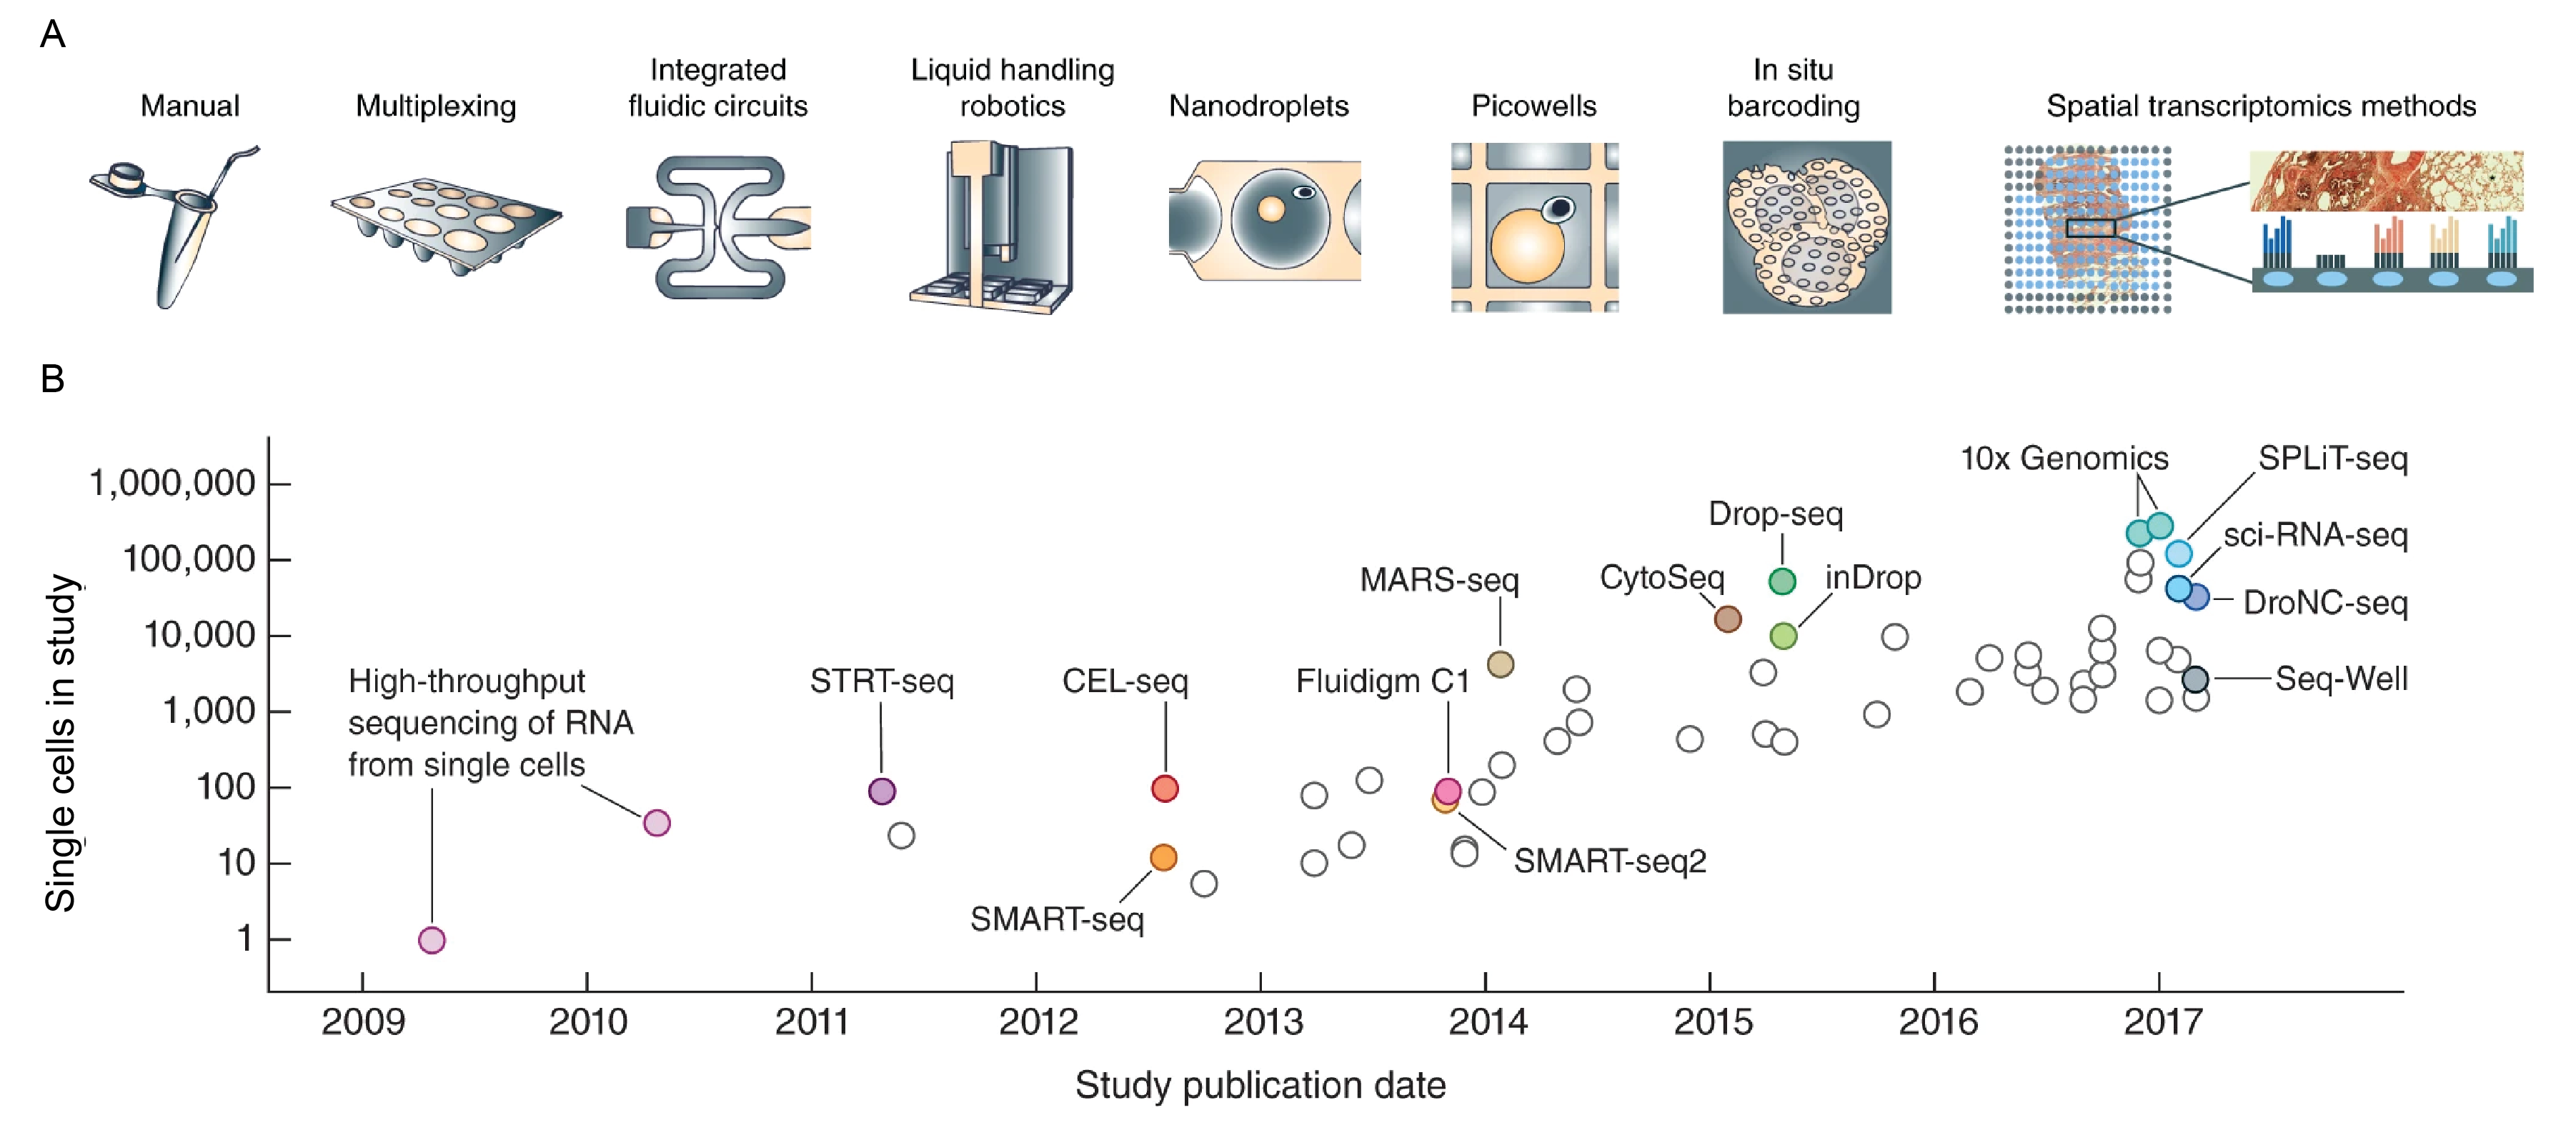
\includegraphics[width=\linewidth]{Chapter1/Fig/F1-5-02.png}
    \caption[Development and scaling of single-cell technologies]{\textbf{Development and scaling of single-cell technologies. (A)} The key technological developments enabling the profiling of large numbers of cells in parallel by single-cell transcriptomics. From initial manual methods allowing the analysis of only few cells to in situ barcoding which increased the throughput to hundreds of thousands of cells. The latest developments in spatial methods integrate the spatial location as well. \textbf{(B)} Cell numbers in representative publications ordered by publication date with key technologies highlighted. \textit{This figure is adapted from} \textbf{\cite{aldridge_single_2020,svensson_exponential_2018}}. }
    \label{fig:chp1_scrna-1}
\end{figure}

Therefore, there has always been great interest in detailing the transcriptional profile at a single-cell level, thereby identifying previously unknown or rare cell populations and studying their frequency compositions as well as investigating the dynamic gene expression patterns and understand the regulatory relationships between genes. With the development of \gls{scr}, this was finally feasible, and this method has revolutionized the field of biology \textbf{(Fig. \ref{fig:chp1_scrna-1} A)}. The very first examples of bona fide single-cell transcriptomics was the study of few mouse primordial germ cells \textbf{\cite{tang_mrna-seq_2009}}. Since then, the field of single-cell biology has developed at breakneck pace, moving from manual collection of few dozens of individual cells to hundreds or thousands of cells automatically \textbf{(Fig. \ref{fig:chp1_scrna-1} A)}. This exponential scaling in cell numbers that can be analyzed simultaneously has almost followed a \textbf{Moore’s Law of single-cell genomics} \textbf{(Fig. \ref{fig:chp1_scrna-1} B)} \textbf{\cite{aldridge_single_2020}}, and recent studies have been able to sequence millions of single cells. Single-cell transcriptomics is now routinely applied to explore the heterogeneity of cell populations, study developmental \textbf{\cite{cao_single-cell_2019,la_manno_molecular_2021}} and disease mechanisms \textbf{\cite{jordao_single-cell_2019,he_single-cell_2021}} and infer regulatory networks \textbf{\cite{wang_cell-type-specific_2020,fei_systematic_2022}} and cellular interactions \textbf{\cite{cherry_computational_2021,shamsi_comprehensive_2023}}. 

% and has been utilized to create reference atlases of healthy human tissues and systems \textbf{\cite{regev_human_nodate}}, mice \textbf{\cite{han_mapping_2018,fei_systematic_2022,wang_construction_2023,the_tabula_sapiens_consortium_tabula_2022}}, fruit fly \textbf{\cite{li_fly_2022}} and non-human primates \textbf{\cite{han_cell_2022,qu_reference_2022}}. It has also expanded our understanding of immune responses \textbf{\cite{stubbington_single-cell_2017,szabo_single-cell_2019,cui_dictionary_2024}}, disease mechanisms \textbf{\cite{miranda_single-cell_2023,mathys_single-cell_2019,li_cancer_2022}}, and is revolutionizing plant biotechnology \textbf{\cite{kaur_single-cell_2024}}. As single-cell technologies continue to advance, they promise to unearth even deeper insights into the cellular underpinnings of life, disease, and development.

%\clearpage

\subsection{A typical \glslink{scr}{scRNA-seq} experiment}
%\colorbox{pink}{missing figure} \colorbox{red}{missing references}\\
\label{sec:scrna_typical}
\par A typical experiment to generate single-cell gene expression data from a biological sample involves several key steps designed to capture and analyze the transcriptomic information: 
\begin{enumerate}
\item Tissue dissociation
\item Single-cell isolation
\item Library construction and 
\item Sequencing 
\end{enumerate}

The first step involves collecting the biological sample(s) of interest (e.g., blood, tissues, cell-cultures) and dissociating into individual cells to obtain a single-cell suspension. This can be done by enzymatic digestion and/or mechanical shearing \textbf{\cite{vieira_braga_tissue_2019}}. Additionally, the suspension can be purified to exclude dead cells or debris and can be further enriched for cell-types of interest. Individual cells are then isolated and sorted into separated containers or wells by manual picking, \textbf{\cite{tang_mrna-seq_2009,kalisky_brief_2018,guo_resolution_2010}}
flow cytometry, \textbf{\cite{hayashi_single-cell_2010,jaitin_massively_2014}}, 
using microfluidic traps, \textbf{\cite{kalisky_brief_2018,treutlein_reconstructing_2014,streets_microfluidic_2014}} 
or encapsulating cells into droplets \textbf{\cite{kalisky_brief_2018,klein_droplet_2015,macosko_highly_2015}}. 

\begin{figure}[H]
    \centering
    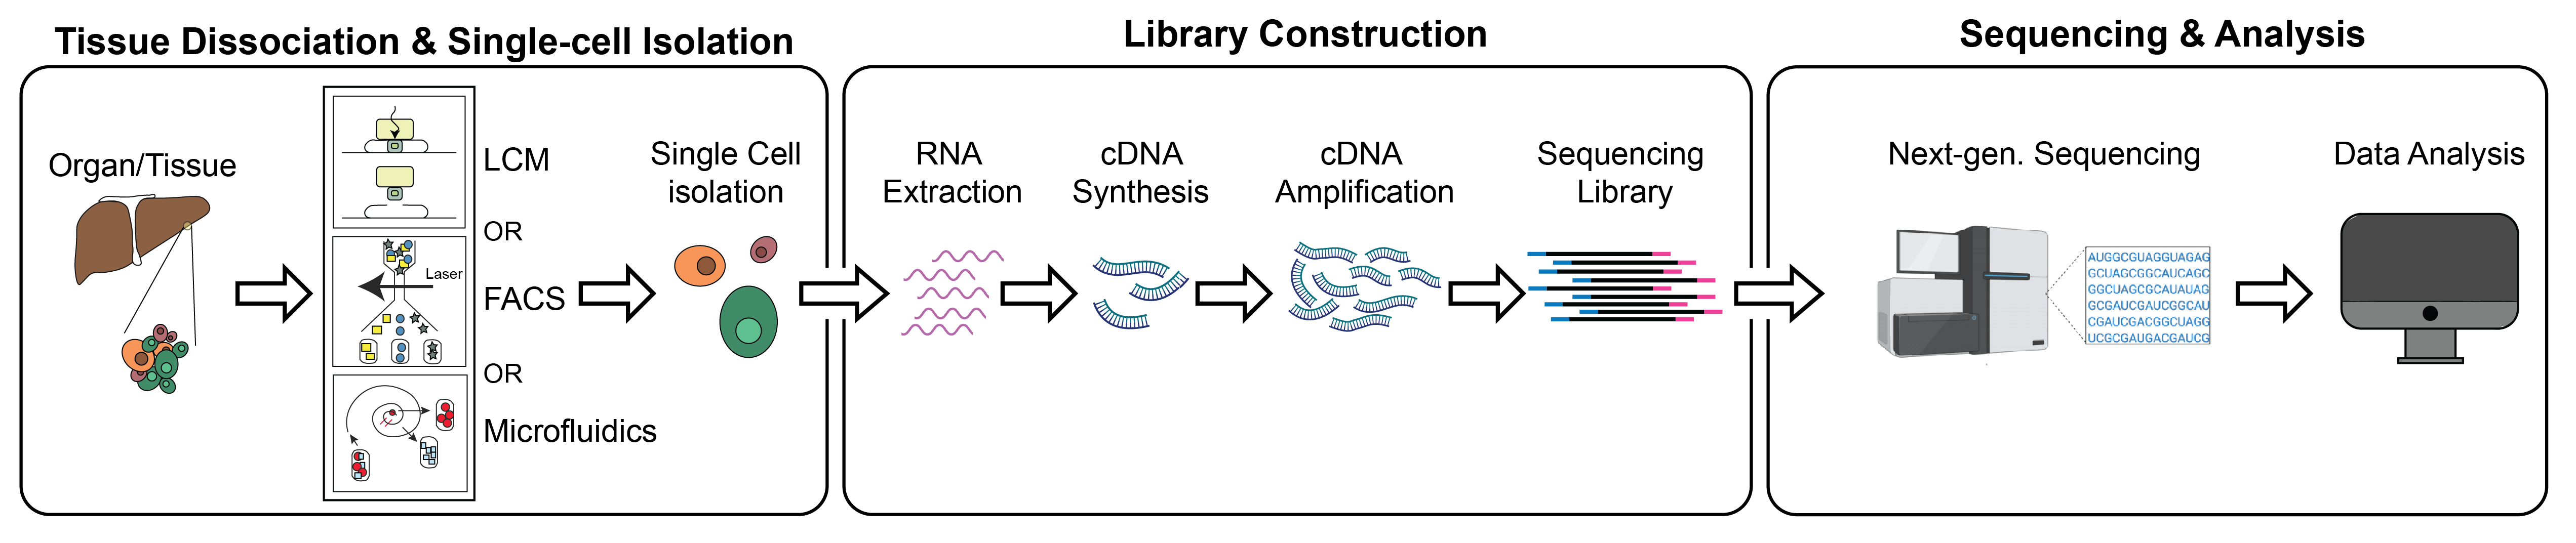
\includegraphics[width=\linewidth]{Chapter1/Fig/F1-5-01.png}
    \caption[A typical single-cell RNA-sequencing experiment]{\textbf{Workflow of a typical \gls{scr} protocol.} The schematic illustrates an overview of steps invovled in a \gls{scr} experiment to generate gene expression data. Abbreviations: LCM, laser capture microdissection; FACS, fluorescence activated cell sorting. \textit{This figure is adapted from Wikipedia. Created with \href{https://www.biorender.com/}{Biorender.com}}.}
    \label{fig:chp1_scrna-2}
\end{figure}

%depending on the desired specificity and/or throughput \textbf{\cite{kalisky_brief_2018}}. 
In this step, errors often lead to the capture of multiple cells in the same partition or the capture of non-viable cells or no cell being captured at all \textbf{\cite{svensson_exponential_2018}}. Once captured, cells are lysed in order to release their RNA content. Poly(T) oligonucleotides allow for capture of poly(A)-tailed RNA. This step enables the cell-specific barcoding of transcripts thereby allowing for sample multiplexing and simultaneous sequencing of all cells. In addition, the transcripts are reverse transcribed into complementary DNA (cDNA) \textbf{\cite{svensson_exponential_2018,haque_practical_2017}}. Since, the starting amount of material is low, the generated cDNA is amplified to prepare sufficient material for subsequent sequencing. Herein, to improve quantification accuracy, \gls{umi} is incorporated to distinguish between the amplified copies of the same \glslink{mrna}{mRNA} molecule and reads from separated \glslink{mrna}{mRNA} molecules from the same gene \textbf{\cite{haque_practical_2017}}. The cDNA is then fragmented, ligated with sequencing adapters and indices to prepare a sequencing library, which can then be sequenced on high-throughput sequencing platforms \textbf{\cite{svensson_exponential_2018,haque_practical_2017}}.\\
\par \gls{scr} protocols can either be full-length which provides full-length transcript data or 3'/5'- end. Full-length sequencing allows for the detection of alternative splicing events and studying genetic alternations such as SNPs, whereas 3'/5'- end is more cost-effective and allows for the incorporation of \glspl{umi} \textbf{\cite{baran-gale_experimental_2018}}. A brief list of commonly used \gls{scr} protocols can be found in \textbf{Table \ref{tab:chp1_scprotocols}}.

\begin{table}[t]
\renewcommand{\arraystretch}{1.2} % More space between rows
\centering
  \caption[Commonly used \gls{scr} protocols]{Commonly used \gls{scr} protocols}
  \label{tab:chp1_scprotocols}
  \begin{tabularx}{\textwidth}{C C C C C}
    \hline
  \rowcolor{headerblue}
    \textbf{Protocol} & \textbf{Type} & \textbf{Platform} & \textbf{Throughput} & \textbf{Reference} \\
    \hline
    MARS-seq & 3'-end & Plate-based & $10^2$ - $10^3$ & \textbf{\cite{jaitin_massively_2014}} \\
    \hline
    Drop-seq & 3'-end & Droplet & $10^3$ - $10^4$ & \textbf{\cite{macosko_highly_2015}} \\
    \hline
    C1 Fluidigm & Full-length & Microfluidics & $10^2$ - $10^3$ & \textbf{\cite{pollen_low-coverage_2014}} \\
    \hline
    Smart-Seq2 & Full-length & Plate-based & $10^2$ - $10^3$ & \textbf{\cite{picelli_smart-seq2_2013}} \\
    \hline
    10x Chromium & 3'/5'- end & Droplet & $10^3$ - $10^4$ & \textbf{\cite{zheng_massively_2017}} \\
    \hline
    
    
  \end{tabularx}

\end{table}



\subsection{10x Genomics}
% \colorbox{pink}{missing figure} \colorbox{orange}{incomplete text} \colorbox{red}{missing references}\\
\label{sec:scrna_10x}
\par The commercially available 10x Genomics Single Cell 3’ v3 protocol is a sensitive, microfluidic-droplet based approach, wherein dissociated cells are encapsulated with oil, reverse transcription (RT) reagents and gel beads containing barcodes into individual reaction vesicles called \gls{gem}. Each barcode consists of a sequencing adapter and primer; a 16 \gls{bp}  barcode sequence and a 12\gls{bp} \gls{umi}, together forming the 28\gls{bp} Read-1; and the poly(dT) oligotide to capture the poly(A) \glslink{mrna}{mRNA}. The \gls{gem}s are fused with the cells in the microfluidic channels of the chip, thereby capturing thousands of cells in a short period of time. The cells are loaded at a low concentration to maximize the number of \gls{gem}s containing single cells, thereby ensuring a low multiplet rate. Once captured, the lysis of cells begins instantaneously and the \glslink{mrna}{mRNA} molecules of the cell are released and captured by the polydT barcode. After RT, each \glslink{cdna}{cDNA} molecule contains the transcript-specific \gls{umi} and \gls{gem}-specific barcode, allowing for subsequent demultiplexing. The \glslink{cdna}{cDNA} is pre-amplified to prepare the libraries for sequencing \textbf{(Fig. \ref{fig:chp1_10xgenomics})}. The gene expression profiling by 10x Genomics Chromium sequences only the 3’ end of the transcript thereby allowing for efficient \glslink{mrna}{mRNA} quantification at the cost of lower sequencing depth. The sequencing model for 10x libraries is based on sequencing both ends of a fragment. This is also known as paired-end sequencing, and it produces twice the amount of reads as single-end sequencing, and allows for the accurate alignment of reads \textbf{\cite{danielski_guidance_2023, noauthor_paired-end_nodate}}.

\begin{figure}[H]
    \centering
    
\includegraphics[width=\linewidth]{Chapter1/Fig/F1-5-03.png}
    \caption[Single-cell sequencing with 10x Genomics Chromium]{\textbf{Single-cell sequencing workflow exemplified by 10x Genomics Chromium platform.} Cells from cell cultures, tissues or individuals are dissociated into a single-cell suspension which is loaded onto a microfluidic chip, and cells are partitioned into \glspl{gem} droplets that contain the barcoded gel beads and reagents for \gls{rt}. After cell lysis, the beads capture the \glslink{mrna}{mRNA} molecules and \gls{rt} generates \glslink{cdna}{cDNA} tagged with a 10x barcode to identify the cell and \gls{umi} to label the \glslink{mrna}{mRNA} transcript. The pooled \glslink{cdna}{cDNA} is amplified to generate sequencing libraries containing the sequencing adapters and a sample index. Abbreviations; BC, barcode; GEMs, gel beads in emulsion; RT, reverse transcription; UMI, unique molecular identifier. \textit{This figure is adapted from \textbf{\cite{swaminath_use_2024}}}}
    \label{fig:chp1_10xgenomics}
\end{figure}

In order to process the Chromium \gls{gem} single-cell data, 10x Genomics also provides a set of analysis pipelines called Cell Ranger to perform end-to-end data analysis. Almost all of the data generated with this technology is first processed via the Cell Ranger \textit{mkfastq} pipeline to demultiplex raw data into FASTQ files. These generated FASTQ files can then be processed with the Cell Ranger \textit{count} pipeline to perform core tasks such as read alignment, filtering, cell and \gls{umi} counting and determine clusters and perform gene expression analysis. For studies involving multiple samples, the data can be combined into a study-wide expression matrix with the Cell Ranger \textit{aggr} pipeline \textbf{\cite{noauthor_what_nodate}}. 

 %As mentioned before, the first read (R1) consists of the 10x \gls{gem}-specific barcode and the transcript-specific \gls{umi} and the second read (R2) consists the actual transcript fragment of \textasciitilde100\gls{bp}. Additionally, the sample index(I1) is sequenced separately and is 8\gls{bp} long.

\clearpage


\subsection{Data analysis methods}
\label{sec:scrna_analysis}
The application of \gls{scr} clearly represents a transformative approach in genomics to dissect the complex heterogeneity of biological tissues at unprecedented resolution. These novel insights into cellular functions, states, interactions and dynamics has been made possible by  a plethora of computational tools and algorithms, developed for the analysis of single-cell data. Currently there are over 1500 tools available in over 30 analysis categories \textbf{\cite{noauthor_scrna-tools_nodate}}, and new tools are being published constantly. These analysis tools are developed in mostly R and Python programming languages, with cross-environment support becoming increasingly commonplace. This allows researchers to seamlessly perform analysis using recommended (or desired) tools, which might only be available in a particular environment. Nevertheless, it is extremely difficult for researchers and beginners to navigate this complex space due to the rapidly expanding number of methods and the rapidly growing sizes of data. Therefore, several reviews are available that summarize the many tools available for a variety of analysis tasks based on the biological question of interest and provide recommendations on best practices of \gls{scr} data analysis whilst discussing existing challenges and outlining future developments in this field \textbf{\cite{zappia_exploring_2018,wu_tools_2020,balzer_how_2021,su_data_2022,ke_single_2022,lueckenmalte_d_current_2019,heumos_best_2023}}.

\vspace{0.2cm}

\begin{Abstract}
\vspace{3mm}
In the following sections, I have attempted to guide the reader through various steps of a typical \gls{scr} analysis pipeline. I have exclusively focused on the description of tasks which I have utilized to analyze the \gls{scr} datasets in Chapter-2 and Chapter-3. I have mostly referred to the guidelines presented in \textit{Current best practices in single-cell RNA-seq analysis: a tutorial} by Luecken et al., 2019 \textbf{\cite{lueckenmalte_d_current_2019}} and \textit{Best practices for single-cell analysis across modalities} by Heumos et al., 2023 \textbf{\cite{heumos_best_2023}}.
\vspace{3mm}
\end{Abstract}

\vspace{3mm}

\par Broadly, the computational algorithms and frameworks for the analysis of scRNA-seq data can be classified into: \textbf{preprocessing pipeline} which deals with raw sequencing data and associated clean-up in order to ensure comparability across samples and \textbf{downstream analyses} which are then applied onto the subsequent pre-processed data. Computational frameworks such as Seurat \textbf{\cite{butler_integrating_2018,stuart_comprehensive_2019,hao_integrated_2021}} and Scnapy \textbf{\cite{wolf_scanpy_2018}} provide top-to-bottom workflows for \gls{scr} data analysis, from initial pre-processing to advanced statistical modeling for interpreting cell populations and scalable pipelines for large datasets. These frameworks are constantly updated to incorporate the latest methodologies and have improved the interoperability between each other, thereby making modular analysis straightforward, and thus offering comprehensive toolkit for single-cell genomics research. 

\clearpage
\subsubsection{From Basecalls to Sequencing Reads}
%\colorbox{pink}{missing figure} \colorbox{red}{missing references}\\

% \begin{wrapfigure}{l}{0.5\textwidth}
%     \centering
%     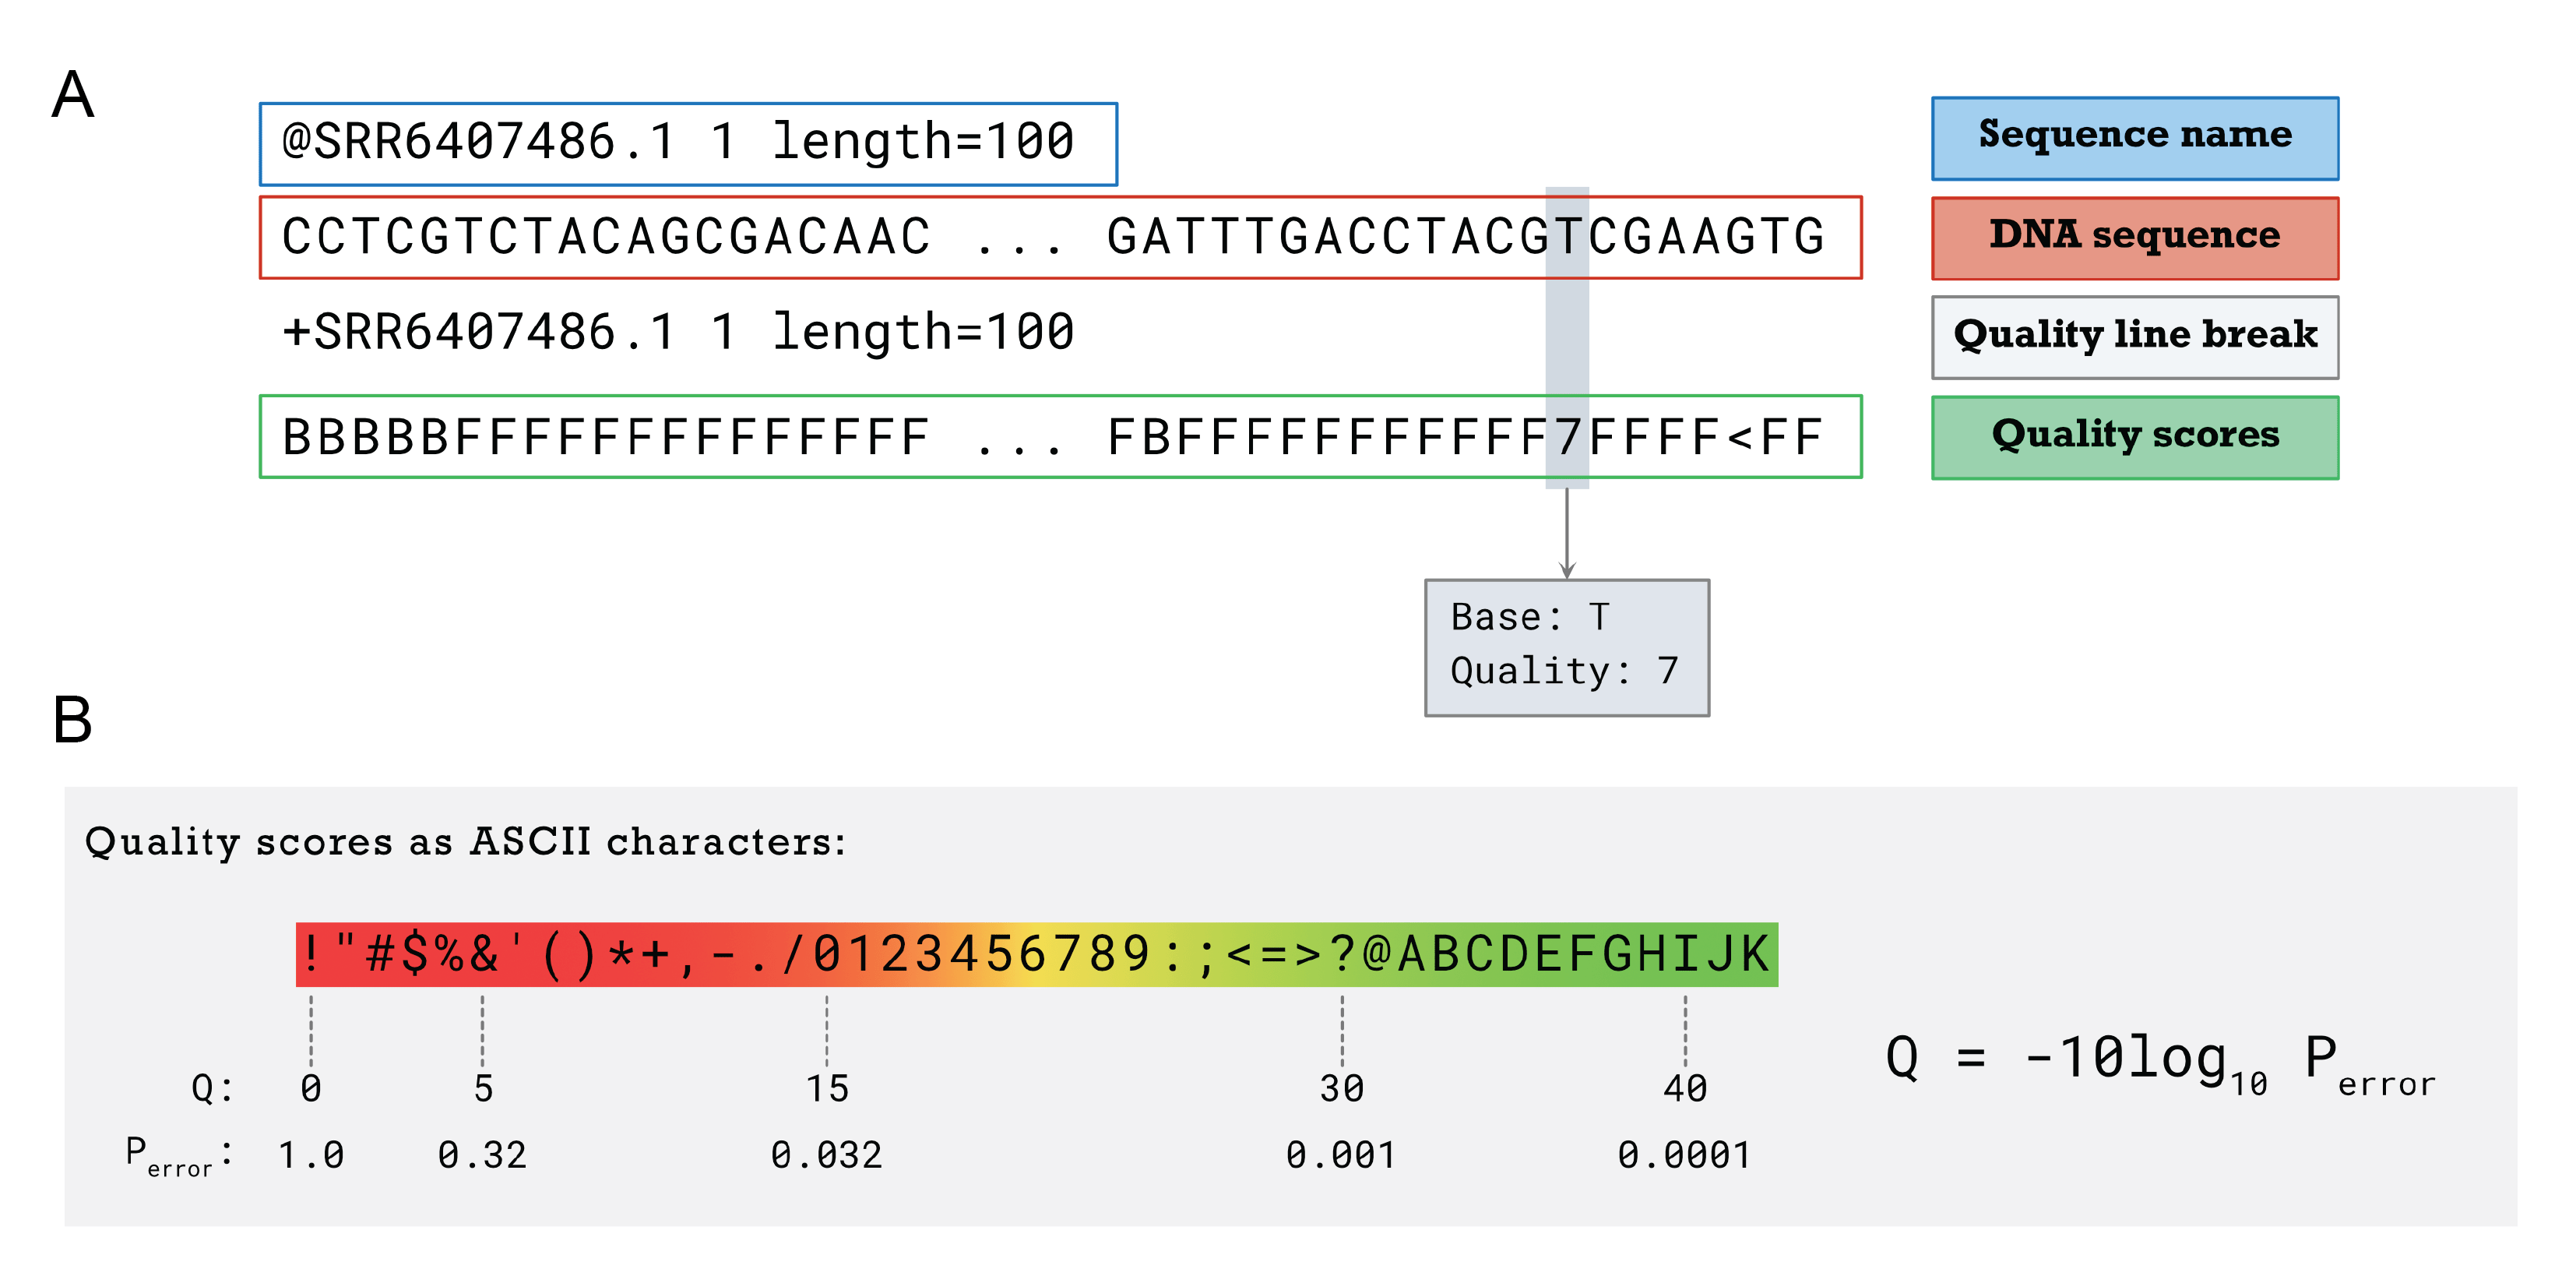
\includegraphics[width=7cm]{Chapter1/Fig/F1-10-01.png}
%     \caption[FASTQ format]{\textbf{The FASTQ file format.}\textbf{(A)} An illustration of the text-based FASTQ format. It uses four lines per sequence: Line-1, begins with `@' symbol, followed by identifier; Line-2, the actual sequence; Line-3, begins with `+' symbol and used as a break; Line-4, the quality scores per base. \textbf{(B)} The quality scores (Q) represented as ASCII-encoded characters. The quality score reflects in a logarithmic scale the probability that a particular base was called incorrectly (\textit{P\textsubscript{error}}). \textit{This figure was adapted from }\textbf{\cite{michal_fastq_2020}}.}
%     \label{fig:chp1_fastq}
% \end{wrapfigure}

% \begin{figure}[H]
%     \centering
%     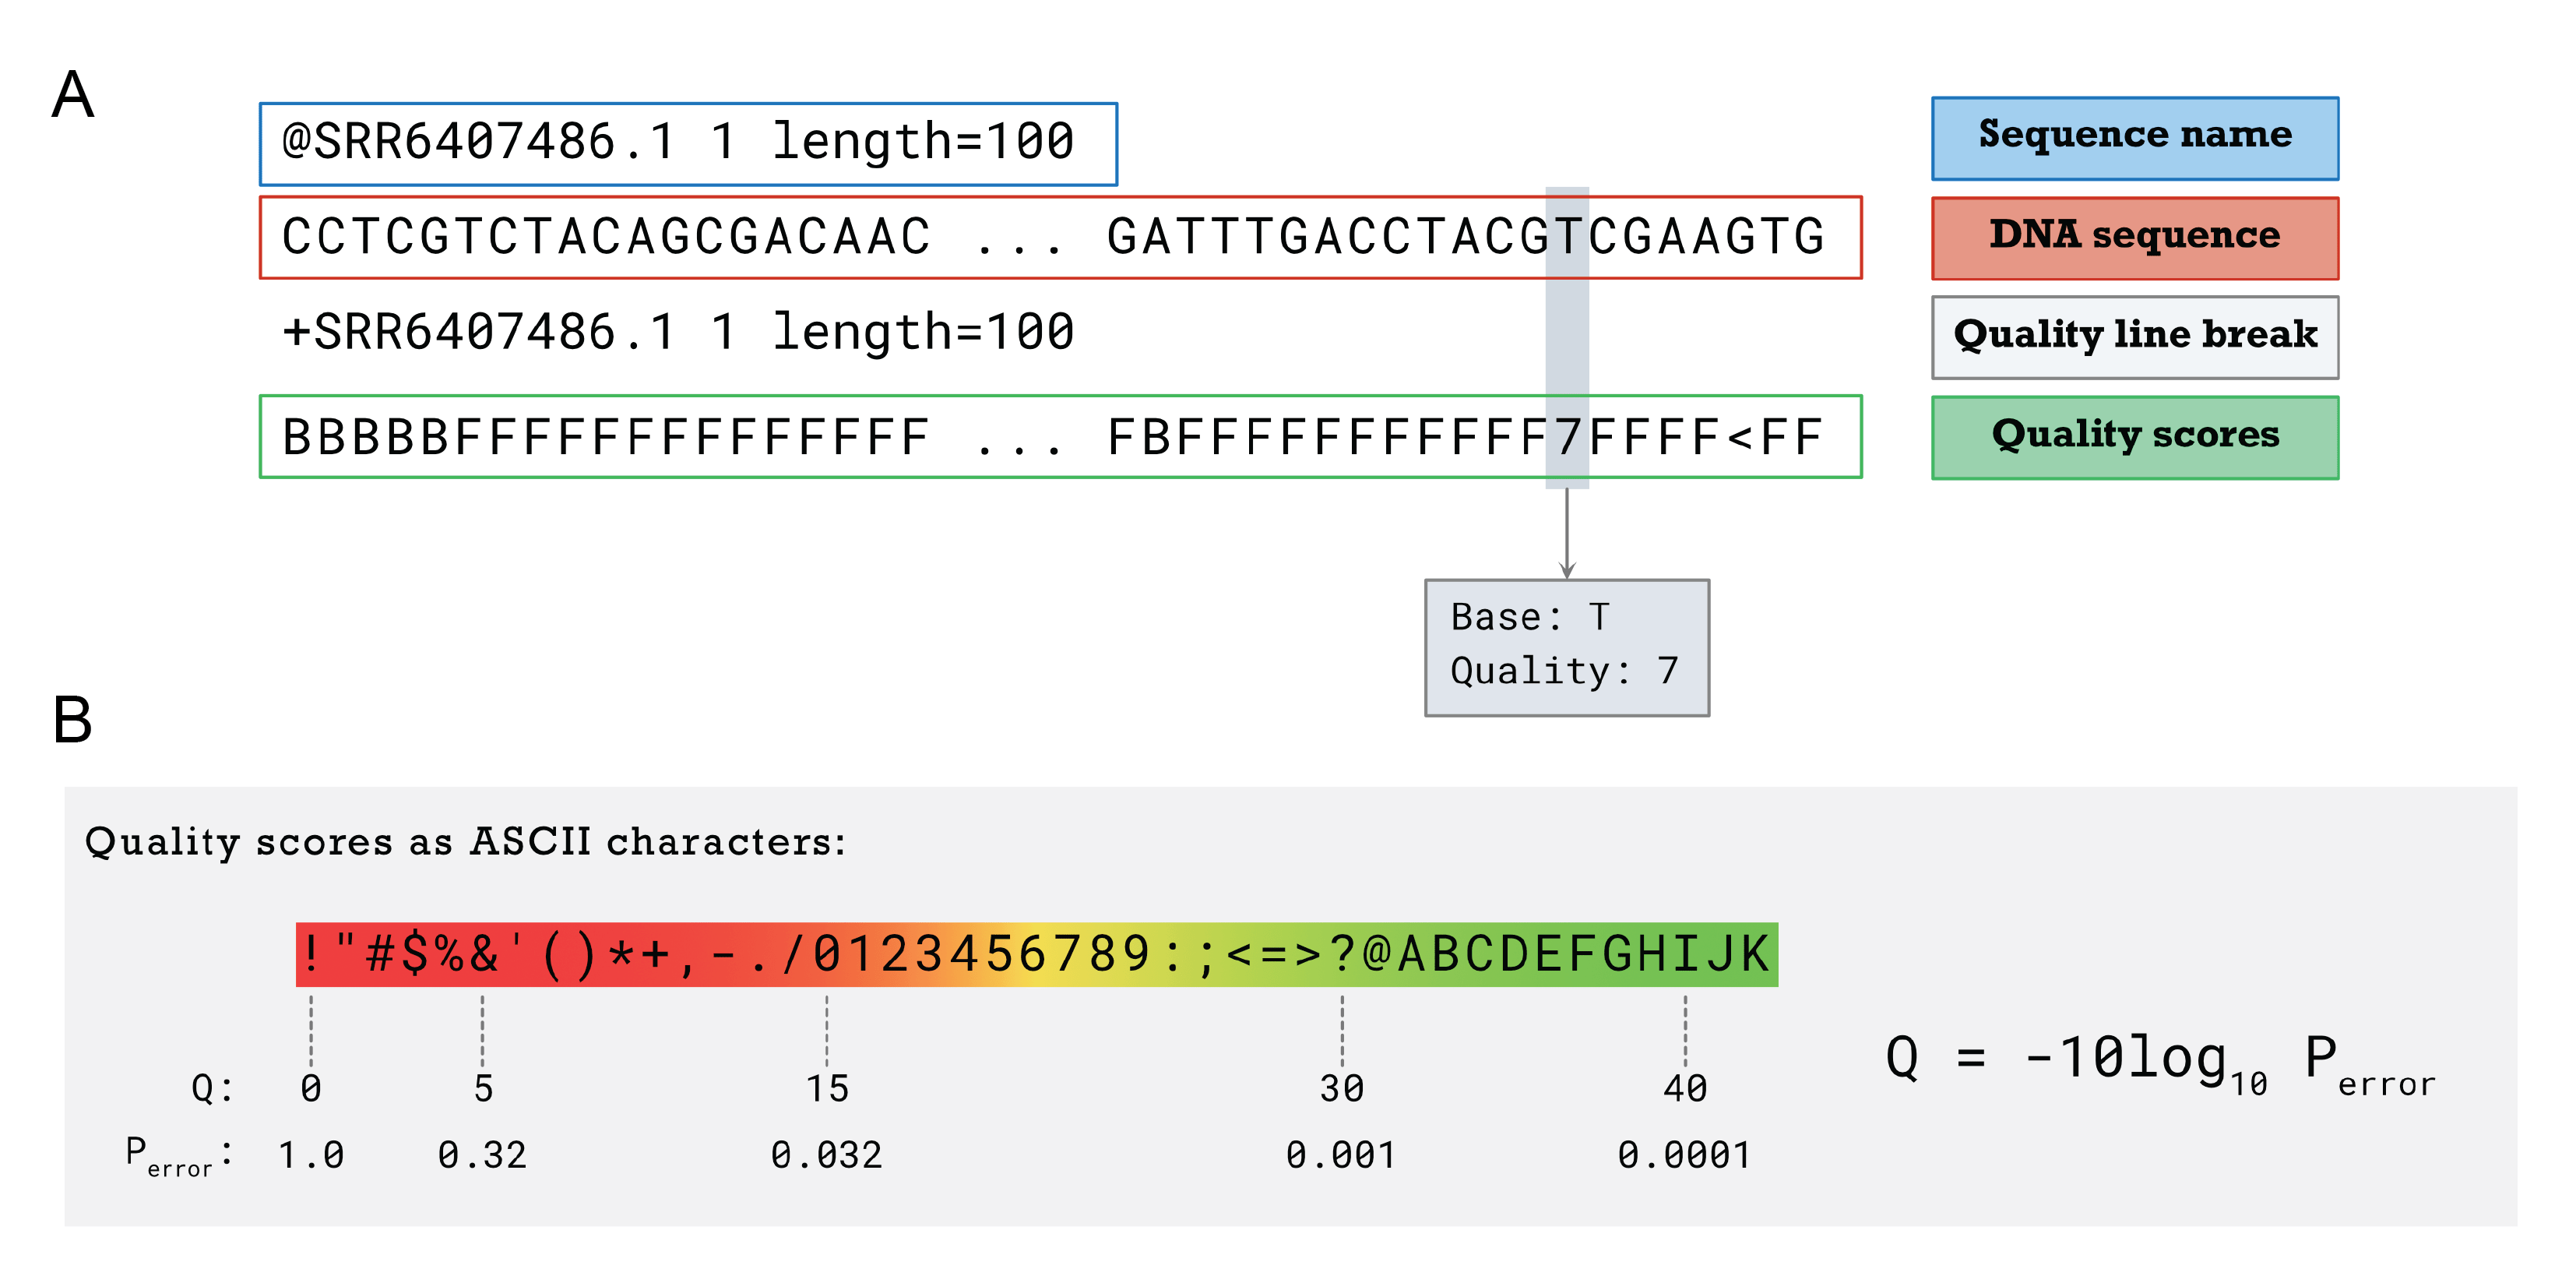
\includegraphics[width=\linewidth]{Chapter1/Fig/F1-10-01.png}
%     \caption[FASTQ format]{\textbf{The FASTQ file format.}}
%     \label{fig:chp1_fastq}
% \end{figure}

The base-calls from a completed sequencing run are converted to text-based sequencing data. This format, called FASTQ, contains the raw sequences in FASTA format and a quality score for each called base. In addition to conversion, a demultiplexing step ensures that the reads are assigned to cells using the barcodes and their respective samples using the sample indices. For a standard 10x Chromium run, these steps can be accomplished with Cell Ranger \textit{mkfastq} pipeline \textbf{\cite{noauthor_generating_nodate}}, which wraps around the Illumina \textit{bcl2fastq} software. Additional evaluation of the sequence quality can be performed in order to ensure that no issues occurred during sequencing \textbf{\cite{andrews_fastqc_2012}}.



\subsubsection{Alignment of Reads}
%\colorbox{pink}{missing figure} \colorbox{red}{missing references}\\

% \begin{wrapfigure}{r}{0.55\textwidth}
%     \centering
%     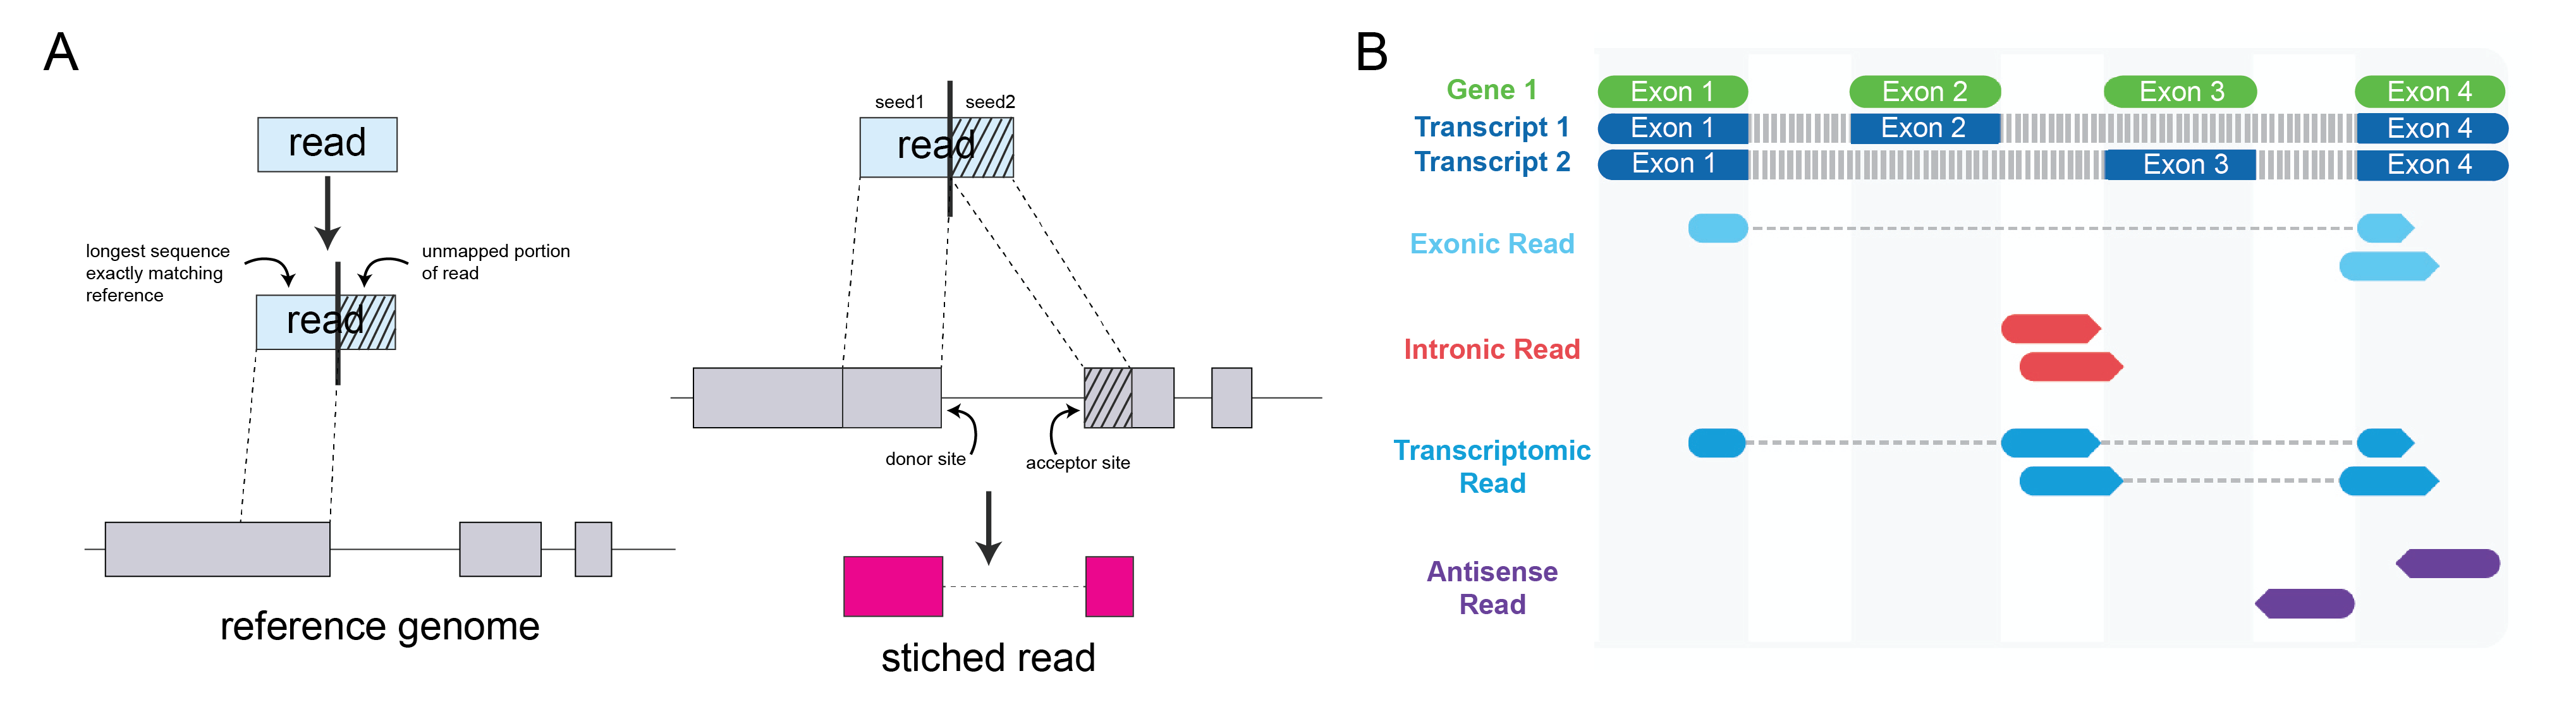
\includegraphics[width=8.5cm]{Chapter1/Fig/F1-10-02.png}
%     \caption[Transcriptome alignment by Cell Ranger]{\textbf{Transcriptome alignment by Cell Ranger \textit{count}.} A simple illustration of how Cell Ranger classifies reads based on how they align to the transcriptome. Cell Ranger carries forward any reads that map in the sense orientation to a single gene - the reads labeled transcriptomic (blue) and ignores antisense reads (purple). \textit{This figure was adapted from }\textbf{\cite{noauthor_cell_nodate}}.}
%     \label{fig:chp1_alignment}
% \end{wrapfigure}

The sorted sequencing reads are first trimmed and then aligned or mapped to a reference genome (mouse / human), wherein the reads are associated with functional genomic elements such as exons, introns or intergenic regions. This is the first step in Cell Ranger \textit{count} pipeline \textbf{\cite{noauthor_running_nodate}}, which uses the STAR aligner to perform splicing-aware alignment of reads \textbf{(Fig. \ref{fig:chp1_alignment} A)} \textbf{\cite{dobin_star_2013}}. The functional annotation of reads is achieved with the help of a transcript annotation file. Cell Ranger performs an additional transcriptome alignment step to determine sense and anti-sense alignments of the confidently mapped exonic and intronic reads \textbf{(Fig. \ref{fig:chp1_alignment} B)} \textbf{\cite{noauthor_cell_nodate}}. Only the reads which map in the sense orientation are carried forward to the next step.\\

\begin{figure}[H]
    \centering
    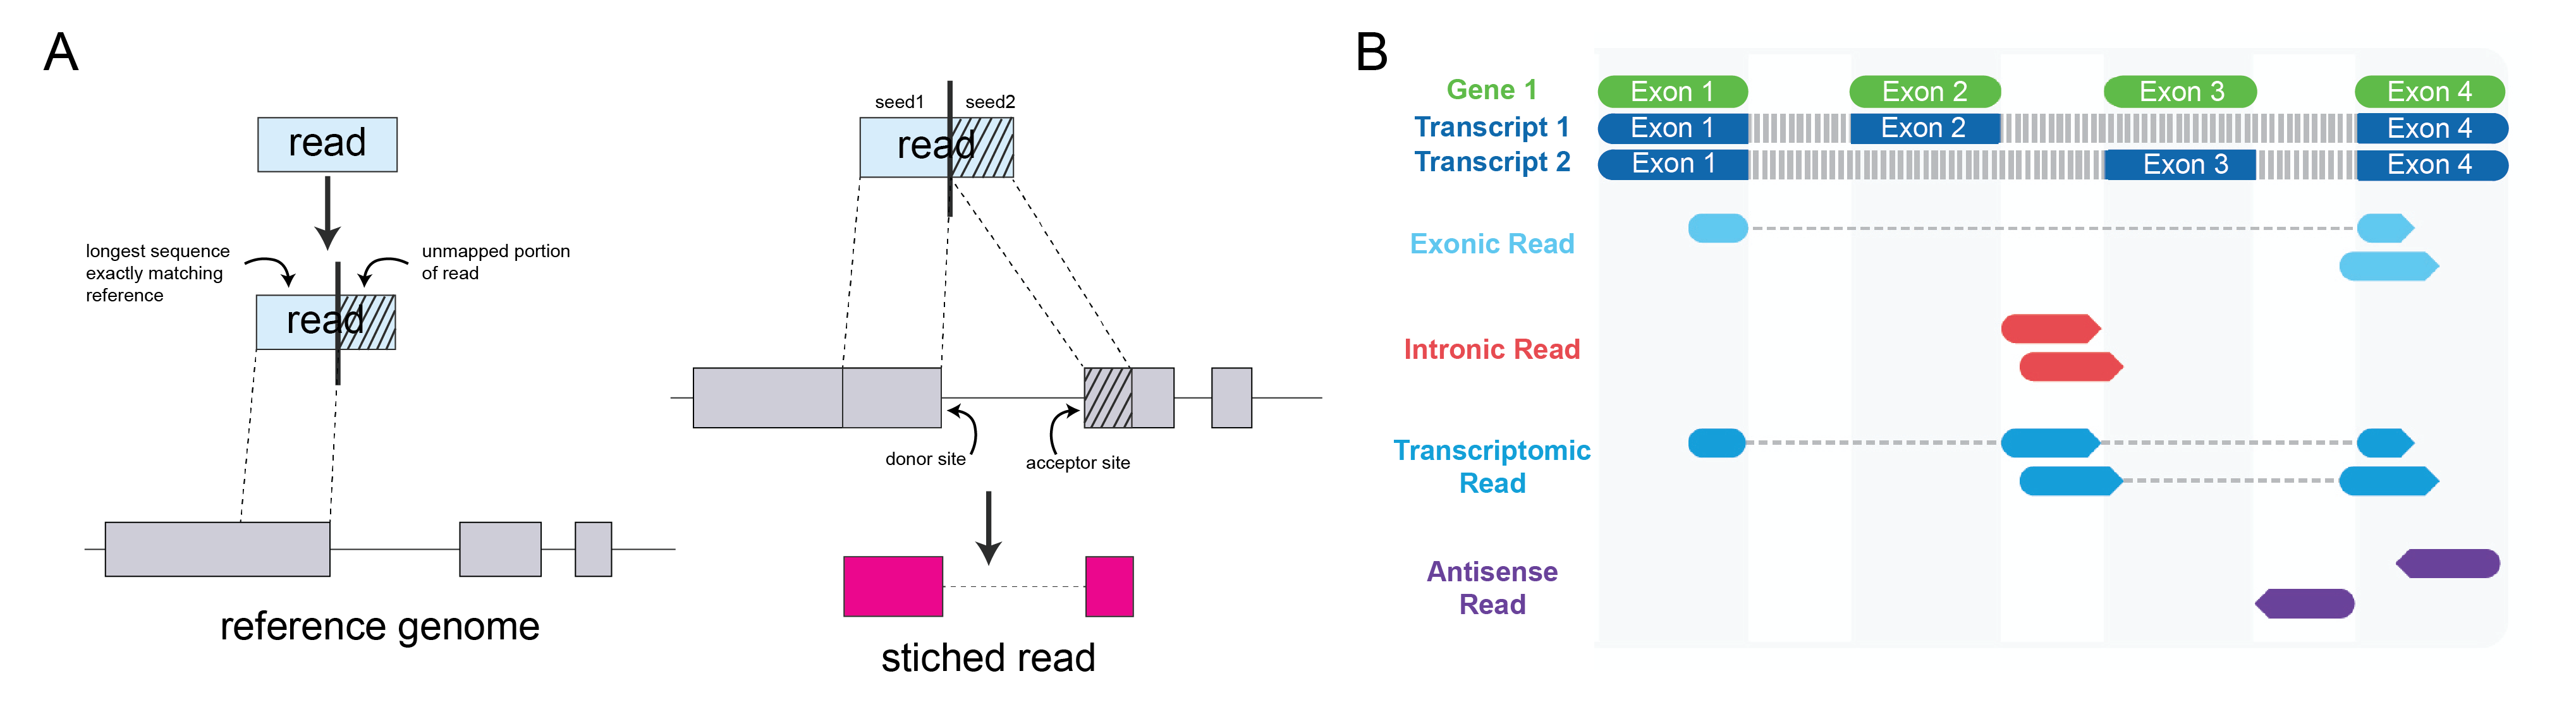
\includegraphics[width=\linewidth]{Chapter1/Fig/F1-10-02.png}
    \caption[Read alignment by Cell Ranger \textit{count}]{\textbf{Read alignment by Cell Ranger \textit{count} pipeline.} \textbf{(A)} The STAR aligner maps reads in a two-step process: initially, it identifies the longest matching sequence (seed1) to the reference genome, followed by aligning any remaining unmapped sequence (seed2). Finally, it stitches these seeds together, considering alignment scores and variations like mismatches and gaps, to reconstruct the read efficiently. \textbf{(B)} A simple illustration of how Cell Ranger classifies reads based on how they align to the transcriptome. Cell Ranger carries forward any reads that map in the sense orientation to a single gene - the reads labeled transcriptomic (blue) and ignores antisense reads (purple). \textit{This figure was adapted from }\textbf{\cite{harvard_chan_bioinformatics_core_hbc_alignment_2017,noauthor_cell_nodate}}.}
   \label{fig:chp1_alignment}
\end{figure}






% \mysidecaption{0.4}{%
% \captionof{figure}[Transcriptome alignment by Cell Ranger]{\textbf{Transcriptome alignment by Cell Ranger \textit{count} pipeline.} A simple illustration of how Cell Ranger classifies reads based on how they align to the transcriptome. Cell Ranger carries forward any reads that map in the sense orientation to a single gene - the reads labeled transcriptomic (blue) and ignores antisense reads (purple). \textit{This figure was adapted from }\textbf{\cite{noauthor_cell_nodate}}.}%
% }
% {%
% 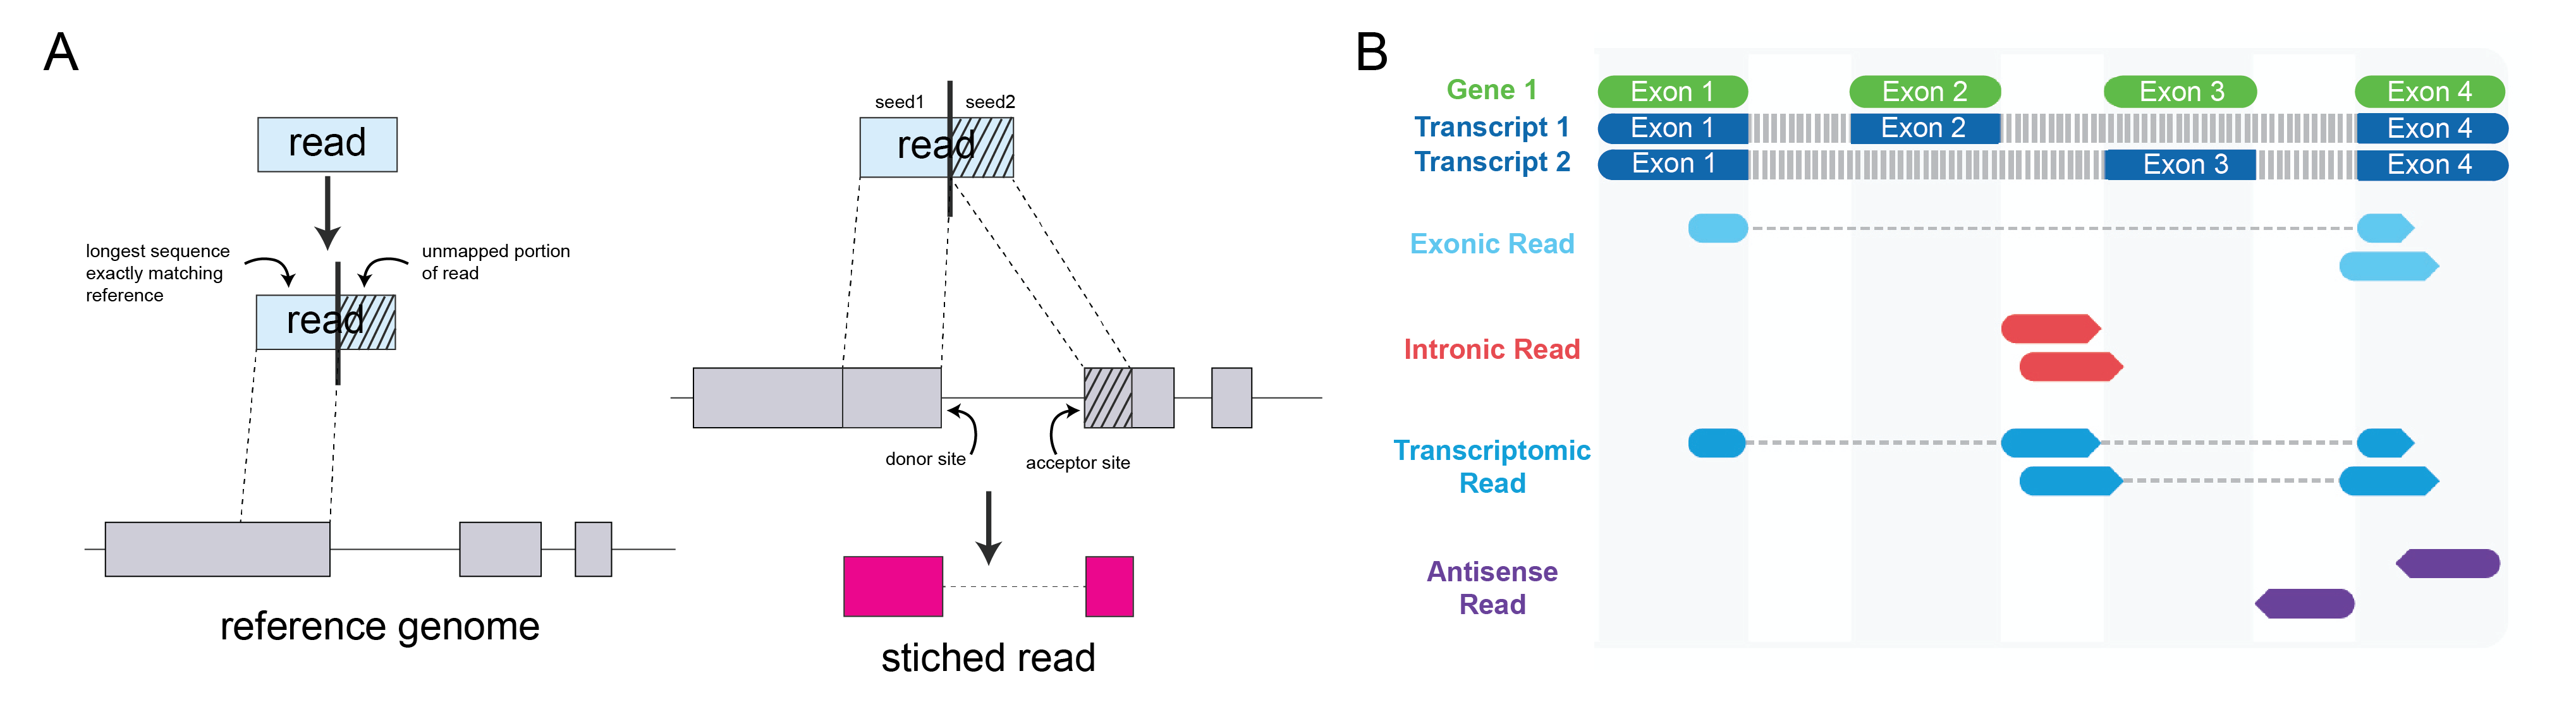
\includegraphics[width=8cm]{Chapter1/Fig/F1-10-02.png}%
% \label{fig:chp1_alignment}
% }%

\clearpage

\subsubsection{\gls{umi} Counting \& Cell Calling}
%\colorbox{pink}{missing figure} \colorbox{red}{missing references}\\
\begin{wrapfigure}{r}{0.5\textwidth}
    \centering
    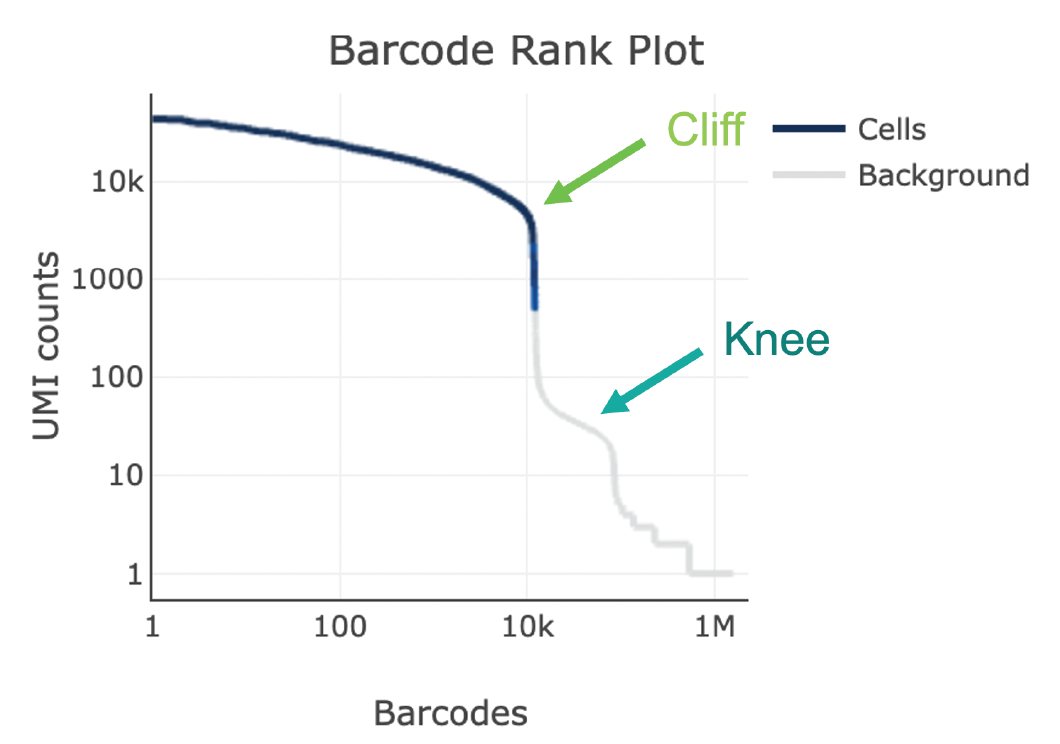
\includegraphics[width=8cm]{Chapter1/Fig/F1-10-03.png}
    \caption[Cell calling by Cell Ranger \textit{count}]{\textbf{Cell calling by Cell Ranger \textit{count} pipeline.} The figure illustrates a Barcode Rank plot that shows all barcodes detected in an experiment, ranked from highest to lowest UMI count. A \textbf{cliff-and-knee} shape in the Barcode Rank plot is indicative of a good quality sample. In this instance, the steep cliff, followed by the plateaued knee, demonstrates that the cell calling algorithm was able to distinguish between intact cells and the background. \textit{This figure is adapted from }\textbf{\cite{noauthor_barcode_nodate}}.}
    \label{fig:chp1_cellcall}
\end{wrapfigure}

Following mapping, Cell Ranger performs barcode correction by comparing the 10x barcodes to a barcode whitelist file for the given chemistry and then correcting the barcodes, which are not in the whitelist and are at the most different from whitelist barcodes by one base. Next, Cell Ranger employs two filtering steps to correct for sequencing errors in the \gls{umi} sequences before generating an unfiltered feature-barcode matrix containing all the observed 10x barcodes and the \gls{umi} counts for genes. As a note, the current versions of Cell Ranger includes both exonic and intronic reads into \gls{umi} counts to maximize sensitivity, whereas previous versions only included exonic reads into \gls{umi} counting. In the cell calling step, Cell Ranger discerns cells with high RNA content by using a cutoff based on the total \gls{umi} counts of each barcode. Following this, the RNA profile of the remaining barcodes is used to determine cells with low RNA content or even empty \gls{gem}s \textbf{\cite{noauthor_cell_nodate}}.


\subsubsection{Quality Control (QC)}
%\colorbox{pink}{missing figure} \colorbox{red}{missing references}

\par To ensure sufficient data quality for downstream analysis of \gls{scr} datasets, additional \gls{qc} steps are required. The most commonly used cell \gls{qc} criteria include:
\begin{enumerate}
    \item \textbf{Library Size} – the total number of transcripts / counts per cell or barcode.
    \item \textbf{Number of Expressed Genes} – the total number of unique genes detected per cell or barcode and
    \item \textbf{Fraction of counts from mitochondrial genes } - cells with unusually high fraction of mitochondrial reads could be dying cells where the cytoplasmic \glslink{mrna}{mRNA} has leaked out due to broken membrane.
\end{enumerate}
\par Due to sample variability, \gls{qc} should be performed independently for each sample and considered in combination to avoid misinterpreting biological signals. The popular scRNA-seq data analysis packages such as Seurat \textbf{\cite{butler_integrating_2018,stuart_comprehensive_2019,hao_integrated_2021}} or Scanpy \textbf{\cite{wolf_scanpy_2018}} provide default settings for excluding cells and genes based on these metrics. Additional tools like Scrublet \textbf{\cite{wolock_scrublet_2019}}, DoubletFinder \textbf{\cite{mcginnis_doubletfinder_2019}} and DoubletDecon \textbf{\cite{depasquale_doubletdecon:_2019}} can be used to filter cells with unusually high counts and a large number of genes as they could represent potential doublets or multiplets, and methods like SoupX \textbf{\cite{young_soupx_2020}} and CellBender \textbf{\cite{fleming_unsupervised_2023}} correct for ambient \glslink{mrna}{mRNA} contamination \textbf{(Fig. \ref{fig:chp1_scrna-workflow} A)}.

% \textit{Firstly}, It is important to note that if the distribution of these QC covariates are different across samples (in case of a multi-sample study), it is recommended to perform individual QC and determine thresholds independently for each sample, in order to account for quality differences across samples. \textit{Secondly}, the above covariates should not be considered in isolation, as this could lead to misinterpretation of biological signals. Cells with low number of transcripts or counts could represent smaller or quiescent cells, whereas cells with high counts may be larger in size. Therefore, the thresholds for these QC metrics should be set as permissive as possible to avoid losing true cell populations. Cells with unusually high counts and a large number of genes could represent potential doublets or multiplets. These can be filtered out using high thresholds or with doublet detection tools such as Scrublet \textbf{\cite{wolock_scrublet_2019}} or DoubletFinder (see \hyperref[sec:suppnote1]{\textbf{Supplementary Note 1}}). \textit{Thirdly}, different cell-types exhibit specific QC covariate peaks which might require iterative QC steps with a particular consideration for lower thresholding values. In addition to cell filtering, it might be necessary to perform gene filtering in order to exclude genes that are not expressed in more than few cells.\\\\The popular scRNA-seq data analysis packages such as Seurat \textbf{\cite{butler_integrating_2018,stuart_comprehensive_2019,hao_integrated_2021}} or Scanpy \textbf{\cite{wolf_scanpy_2018}}, by default, exclude cells with less than 200 genes detected and exclude genes not expressed in at least 3 cells. Additional QC can be performed in case of background `ambient mRNA’ contamination by freely floating transcripts that could contaminate endogenous expression profiles of cells. These effects can be corrected in droplet-based scRNA-seq datasets using empty droplets to model the ambient mRNA contamination rate, using methods such as SoupX \textbf{\cite{young_soupx_2020}} or CellBender \textbf{\cite{fleming_cellbender_2019}} (see \hyperref[sec:suppnote2]{\textbf{Supplementary Note 2}}).
%\clearpage

\subsubsection{Normalization \& Scaling}
%\colorbox{pink}{missing figure}\\

%Compared to bulk \gls{rnaseq}, data from \gls{scr} is embedded with technical noise as a result of capture inefficiency, amplification bias or varying sequencing depths across cells or samples. Therefore, to allow for gene expression comparison between cells or samples, 

The normalization of \gls{scr} data addresses technical variations such as dropout events or zero-inflation thereby allowing for the comparison of gene expression between cells. While normalization methods available for bulk \gls{rnaseq} data have been applied to \gls{scr}, the specific sources of variation have encouraged the development of \gls{scr} specific normalization-methods. Seurat \textbf{\cite{butler_integrating_2018,stuart_comprehensive_2019,hao_integrated_2021}} and Scanpy \textbf{\cite{wolf_scanpy_2018}} normalize each cell by dividing the feature counts by total counts for that cell. Following this, the values are multiplied by a cell-specific normalization factor (termed scale factor) to adjust the raw gene expression. Finally, the normalized data is \textit{log} transformed, \begin{math}log(x+1)\end{math}, in order to stabilize the variance and to reduce the data skewness. The use of \textbf{1} as a pseudo-count addresses the zero counts in the dataset. A more recent approach utilizes pearson residuals, by using a regularized negative binomial regression model \textbf{\cite{hafemeister_normalization_2019}}. Similar to normalizing cellular counts, gene counts across all the cells can be normalized or scaled to have zero mean and unit variance. Currently, there is no consensus on whether to perform scaling over genes or not. While, Seurat \textbf{\cite{stuart_comprehensive_2019,hao_integrated_2021}} applies gene scaling, Scanpy \textbf{\cite{wolf_scanpy_2018}} refrains from doing so in order to retain as much biological information from the data as possible \textbf{(Fig. \ref{fig:chp1_scrna-workflow} A)}.

\subsubsection{Feature Selection}
%\colorbox{pink}{missing figure} \colorbox{red}{missing references}\\
% As previously discussed, scRNA-seq data are subject to inherent noise due to stochastic nature of gene expression being captured in conjunction with low mRNA capture efficiency. To reduce this intrinsic noise, it is necessary to exclude non-informative parts of the data from downstream analysis. 
Feature selection is one of the most crucial steps in scRNA-seq data analysis. The underlying theme of this step is to select the most biologically \textbf{informative} genes in the dataset. The selection of the genes is performed by fitting a gene-wise model using the coefficient-of-variation versus the mean expression, and identifying the genes which violate the assumption of constant expression across all cells. The genes that disperse the most around the mean are selected and are termed as \glspl{hvg} or \glspl{hvf} \textbf{(Fig. \ref{fig:chp1_scrna-workflow} A)}. %Thus, this step reduces the dimensionality of the dataset to only the \glspl{hvg}. 
While,Seurat \textbf{\cite{butler_integrating_2018,stuart_comprehensive_2019,hao_integrated_2021}}, by default, selects 2000 \glspl{hvg}, this is not fixed in Scanpy \textbf{\cite{wolf_scanpy_2018}} and is dependent on parameter values for dispersion and mean cut-offs, thereby allowing for additional flexibility in \glspl{hvg} selection.

\subsubsection{Batch Correction \& Data Integration}
%\colorbox{pink}{missing figure} \colorbox{orange}{incomplete text} \colorbox{red}{missing references}\\

Batch effects present a central challenge in most scRNA-seq analysis and systematic differences between batches can confound biological signals of interest and provide misleading conclusions. Therefore
%, in order to eliminate or minimize such technical (sample handling, experimental protocols or sequencing depths) or biological (donor variation, tissue or sampling location) confounders while preserving true biological variability, 
efficient removal or minimization of batch effects is fundamental. However, batch effects can arise at various levels and the choice of the levels to retain or remove the variation ultimately depends on the goal of the integration task and the intended downstream analyses.\\\\
Data integration is a fundamental step in scRNA-seq analysis workflow and serves to minimize batch effects and to consolidate datasets from different conditions or experiments. 
%The two primary goals of data integration are: \textbf{(i)} to minimize the batch effects across the samples or datasets, and \textbf{(ii)} to analyze data in an unified framework. 
Data integration strategies ensure that downstream analysis accurately reflect biological variance, allowing for discoveries that would not be achievable with isolated datasets \textbf{(Fig. \ref{fig:chp1_scrna-workflow} A)}.  % the choice of batch covariate would determine which level of variation would be retained and which would be removed. This, ultimately depends on the goal of the integration task and the intended downstream analyses to be performed.\\\\
The anchor-based canonical correlation analysis (CCA) implemented as part of Seurat \textbf{\cite{stuart_comprehensive_2019}} workflow, is one of the most popular methods for batch effects correction and data integration in \gls{scr} datasets. For large datasets, Seurat offers alternative workflows in order to improve efficiency and runtimes. \gls{scr} datasets can also be integrated with Scanpy via the \textbf{ingest} workflow. %Both, CCA and ingest are \gls{pca}-based methods. 
While, CCA learns a joint representation to integrate the datasets, ingest preforms asymmetric dataset integration between annotated reference dataset and new data. A recent benchmarking compared several \gls{scr} data-integration methods across different metrics of batch correction and biological conservation \textbf{\cite{luecken_benchmarking_2021}}.\\
% Several data integration (or batch correction) methods have been developed and depending on the complexity of the integration task \hl{....}

Additional data corrections steps such as: \textbf{(i)} biological regression to remove the effects of cell-cycle using a list of marker genes  \textbf{\cite{macosko_highly_2015}}, to regress out the expression of mitochondrial or ribosomal genes; \textbf{(ii)} technical regression of counts per cell in order to make the cells more comparable to each other are also routinely performed to improve the accuracy of downstream analyses and facilitate clearer understanding of underlying cellular processes. 

% A normalized scRNA-seq dataset might still contain additional variability, therefore necessitating additional data correction of technical and/or biological covariates to improve the accuracy of downstream analyses and facilitate clearer understanding of underlying cellular processes. Data correction can be performed as: 
% %which can confound the true biological signal. . 
% %Data correction is usually performed in the form of linear regression to remove confounding effects. The most commonly performed biological regression is to remove the effects of cell cycle on the transcriptome, based on a list of marker genes available from literature \textbf{\cite{macosko_highly_2015}}. Apart from cell-cycle, other biological covariates such as expression of mitochondrial genes or ribosomal genes can also be regressed out. In addition to biological effects, technical covariates such as counts per cell can also be regressed out in order to make the cells more comparable to each other. 
% The linear regression method is implemented in Seurat \textbf{\cite{butler_integrating_2018,stuart_comprehensive_2019,hao_integrated_2021}} and Scanpy \textbf{\cite{wolf_scanpy_2018}} workflows.\\\\


\subsubsection{Dimensionality Reduction (DR) \& Visualization}
%\colorbox{pink}{missing figure} \colorbox{green}{text cleanup}\\
\gls{dr} is a crucial step in every scRNA-seq data analysis in order to simplify the complex, high-dimensional gene expression data. The \gls{dr} algorithms project the data onto a low-dimensional space while preserving the most significant information and the essential structures in the dataset. These algorithms also make the computational analysis more tractable \textbf{(Fig. \ref{fig:chp1_scrna-workflow} A)} \textbf{\cite{lueckenmalte_d_current_2019}}. 
The most frequently used \gls{dr} method is \gls{pca} \textbf{\cite{pearson_liii_1901}} which is a linear, summarization approach to DR \textbf{\cite{lueckenmalte_d_current_2019,heumos_best_2023}}. 
%PCA assumes linear relationships between genes and decomposes the data into orthogonal vectors or components, thereby compressing and summarizing to maximize the residual variance. Typically, PCA reduces a dataset to its top N components, wherein the variance of the data decreases with successive components. The “N” can be determined either by an “elbow-plot” or by using the jackstraw method \textbf{\cite{macosko_highly_2015,lueckenmalte_d_current_2019,chung_statistical_2015}}. It is important to note that the variation explained by PCA might not necessarily be biologically meaningful and the components might correlate with technical factor(s) \textbf{\cite{finak_mast_2015}}. Therefore, the components should be scrutinized for any unwanted correlation and discarded when necessary. 
\gls{pca} is computationally efficient and is primarily used as a pre-processing step for visualization, clustering or other downstream analysis tasks \textbf{\cite{lueckenmalte_d_current_2019}}. Complementing \gls{pca}, non-linear \gls{dr} methods such as \gls{tsne} \textbf{\cite{maaten_visualizing_2008}} or \gls{umap} \textbf{\cite{mcinnes_umap_2020}} are utilized for the visualization of \gls{scr} datasets \textbf{\cite{lueckenmalte_d_current_2019,heumos_best_2023}}. \gls{tsne} and \gls{umap} work in similar way by making similar data-points (cells) attract each other and push dissimilar points away from each other. The loss functions in both algorithms are minimized using gradient descent. 
%UMAP differs from tSNE in the use of Laplacian eigenmaps (LE) for its initialization step, whereas tSNE algorithm performs random initialization. While, it is perceived that UMAP is able to offer a more faithful representation of the global structure, this can be attributed to the choice of initialization. tSNE with informative initialization, such as PCA, performs as well as UMAP with LE initialization \textbf{\cite{kobak_initialization_2021}}. 
However, \gls{umap} is computationally efficient and can easily be scaled to large datasets and has therefore become the preferred method of DR and visualization in the single-cell community \textbf{\cite{kobak_initialization_2021,becht_dimensionality_2018}}. In addition to the above methods, \gls{paga} \textbf{\cite{wolf_paga_2019}} provides an interpretable graph-like map which can adequately approximate the topology of the data and provide coarse visualization of clusters in the single-cell data.

\subsubsection{Clustering \& Cell-type annotation}
%\colorbox{pink}{missing figure}  \colorbox{red}{missing references}  \colorbox{green}{text cleanup}\\
One of the primary results of \gls{scr} analysis is the grouping of single-cells into clusters based on similar transcriptomic profiles that explain the heterogeneity of the data \textbf{(Fig. \ref{fig:chp1_scrna-workflow} B)}. However, clustering of \gls{scr} data is a complex and challenging task due to the high-dimensionality and sparsity of the data combined with little to no knowledge about the number of the clusters. Several different clustering results can be obtained for the same dataset based upon the choice of the clustering method or the underlying parameters. %\footnote{The resolution parameter controls the number of clusters obtained}. 
The two major classes of methods for generating single-cell clusters include : \textbf{(i)} clustering algorithms based on distance metrics such as Euclidean, cosine-similarity or correlation-based distances, and \textbf{(ii)} community detection algorithms like Louvain \textbf{\cite{blondel_fast_2008}} or Leiden \textbf{\cite{traag_louvain_2019}}, which are based on partitioning the \glslink{knn}{\textit{k}NN} graph representation of a single-cell data. The choice of clustering method for \gls{scr} data is crucial and should be tailored to the specific characteristics of the dataset and the biological questions being investigated.\\
% The Louvain algorithm, a community detection method, has been shown to outperform other clustering methods for scRNA-seq data and is used as the default method in Seurat and Scanpy analysis workflows \textbf{\cite{lueckenmalte_d_current_2019,heumos_best_2023,duo_systematic_2020,freytag_comparison_2018}}. The algorithm works by iteratively moving nodes from one community to other in order to increase the modularity of the network. After this, every community is aggregated into a single node and the process is repeated all over again until the modularity cannot be increased any further. However, this can lead to arbitrarily poorly connected communities \textbf{\cite{heumos_best_2023,traag_louvain_2019}}. The Leiden algorithm \textbf{\cite{traag_louvain_2019}} circumvents this issue and is computationally more efficient than Louvain method. Thus, the choice of clustering method for scRNA-seq data is crucial and should be tailored to the specific characteristics of the dataset and the biological questions being investigated.\\\\
\par Once, cell clusters are identified, the next step entails annotating the clusters to obtain biological interpretation. %\st{While, it may seem reasonable to equate clusters to cell-types, it is important to note that cellular identity can be captured along several axes of variation and therefore assigning a single cell-type to a cluster might oversimplify the complex nature of biological diversity in the dataset.} 
On a simplistic level, the clusters are annotated by examining the transcriptomic signatures (marker genes) of individual clusters. The marker genes are identified by comparing two clusters and extracting the up-regulated or down-regulated genes in the clusters of interest. A statistical test, e.g. \textit{Wilcoxon rank-sum} test, is applied to this comparison and further adjusted for multiple testing.  %\footnote{In marker gene detection, it's important to note two things: First, the accuracy of P-values relies on the assumption that cell clusters truly reflect biological groups, which can be problematic since clustering and marker gene identification both use the same gene expression data, potentially leading to inflated P-values. A permutation test can help adjust for this. Second, the identification of marker genes is influenced by the dataset's composition, meaning results may be biased if the dataset lacks diversity. Despite these challenges, top-ranked marker genes remain valuable for identifying cellular identities, but caution is advised, especially in datasets with limited cell variety}
These data-driven marker genes can then be compared against known marker genes from literature, thereby assigning cellular identities to the cluster. To perform this step at scale for the increasingly huge and complex dataset and in the interest of speed, automated annotation methods are now available. With this, the dataset in question (\textbf{query}) can be mapped to existing, related, well-annotated single-cell datasets or large atlases (\textbf{reference}) and the annotations can be transferred from reference to query. This 

\begin{figure}[H]
    \centering
    \includegraphics[width=\linewidth]{Chapter1/Fig/F1-8-01.png}
    \caption[Workflow for pre-processing and analysis of \glslink{scr}{scRNA-seq} data]
    {\textbf{Overview of analysis steps for \gls{scr} data.} \textbf{(A)} Matrices of counts for genes across all cells are obtained from the previous raw data processing pipelines. The count matrices are further corrected for cell-free ambient \glslink{mrna}{mRNA}, excluded of putative cell doublets and filtered for low-quality or dying cells. Next, the count matrices are normalized in order to obtain correct relative gene abundances between cells. The most variably expressed genes across all the cells are selected in the Feature selection step. Different batches or samples in the dataset are integrated in order to obtain a corrected data matrix across samples. \glslink{dr}{DR} techniques are applied to reduce computation burden and noise, and to aid in visualization. \textbf{(B)} The integrated data is organized into clusters which represent groups of cells with similar expression profiles. Based on marker genes, the clusters can be annotated with labels, such as cell-types of interest. Additionally, clusters can also be annotated via query-to-reference mapping in order to transfer annotations from previously annotated scRNA-seq datasets. \textbf{(C)} Further downstream analysis can be performed based on question of interest - composition analysis can reveal shifts in cell-type proportions between conditions; differential expression analysis can reveal up-regulated and down-regulated genes between conditions; gene-set enrichment can identify pathways between conditions. \textbf{(D)} Continuous processes such as cell-type and/or cell-state transitions can be identified via trajectory inference methods and future cell-states can be predicted with RNA-velocity. Further, gene regulatory networks underlying the cell-types and/or cell-states can be identified and expression patterns of ligands and receptors can reveal cell-cell interactions. Abbreviations: Dim, dimension; FC, fold change; Adj. P-value, adjusted P-value; TF, transcription factor; Commun. Prob., communication probability. This figure is adapted from \textbf{\cite{heumos_best_2023,weiler_guide_2022,armingol_deciphering_2021}}.\textit{ Reproduced with permission from Springer Nature.}}
    \label{fig:chp1_scrna-workflow}
\end{figure}
    

% - genes in the clusters of interest. A statistical test, e.g. \textit{Wilcoxon rank-sum} test, is applied to this comparison and further adjusted for multiple testing.  %\footnote{In marker gene detection, it's important to note two things: First, the accuracy of P-values relies on the assumption that cell clusters truly reflect biological groups, which can be problematic since clustering and marker gene identification both use the same gene expression data, potentially leading to inflated P-values. A permutation test can help adjust for this. Second, the identification of marker genes is influenced by the dataset's composition, meaning results may be biased if the dataset lacks diversity. Despite these challenges, top-ranked marker genes remain valuable for identifying cellular identities, but caution is advised, especially in datasets with limited cell variety}
% These data-driven marker genes can then be compared against known marker genes from literature, thereby assigning cellular identities to the cluster. To perform this step at scale for the increasingly huge and complex dataset and in the interest of speed, automated annotation methods are now available. With this, the dataset in question (\textbf{query}) can be mapped to existing, related, well-annotated single-cell datasets or large atlases (\textbf{reference}) and the annotations can be transferred from reference to query. This is also known as \textit{transfer learning} \textbf{(Fig. \ref{fig:chp1_scrna-workflow} B)} and such query-to-reference mapping can be performed by several tools such as Azimuth \textbf{\cite{hao_integrated_2021}} or scArches \textbf{\cite{lotfollahi_mapping_2021}}. Automatic annotation can also be performed with classifier-based methods, which make use of pre-trained classifiers \textbf{\cite{dominguez_conde_cross-tissue_2022,fu_clustifyr_2020}}. In both cases, the quality of annotation is dependent on the quality of the reference data and the model employed.\\\\
is also known as \textbf{transfer learning} \textbf{(Fig. \ref{fig:chp1_scrna-workflow} B)} and such query-to-reference mapping can be performed by several tools such as Azimuth \textbf{\cite{hao_integrated_2021}} or scArches \textbf{\cite{lotfollahi_mapping_2021}}. Automatic annotation can also be performed with classifier-based methods, which make use of pre-trained classifiers \textbf{\cite{dominguez_conde_cross-tissue_2022,fu_clustifyr_2020}}. In both cases, the quality of annotation is dependent on the quality of the reference data and the model employed.\\\\
Hence, cluster annotation is a crucial step for obtaining biologically meaningful insights from \gls{scr} datasets and to understand the composition of the annotated clusters, their functional roles, and ultimately their potential roles in health and disease.


\subsubsection{Cell composition \& Cell abundances}
%\colorbox{pink}{missing figure}\\
At a cellular level, the clustered and annotated \gls{scr} dataset can be used to address conditional changes in the relative proportions of cell-types or clusters in response of biological processes such as development or disease \textbf{(Fig. \ref{fig:chp1_scrna-workflow} C)}. %However, due to several technical and methodological limitations of \gls{scr} such as lack of or low number of experimental replicates and the limited number of cells sequenced from a sample, 
The cell type count data represents relative abundances of all cell-types of a sample or tissue, and is known as compositional data \textbf{\cite{noauthor_compositional_nodate}}. Univariate methods such as \textit{Wilcoxon rank-sum} tests ignore the compositionality of the data, leading to elevated false discovery rates (FDRs) and falsely perceiving statistically sound cell-type shifts \textbf{\cite{noauthor_compositional_nodate}}. Single-cell specific methods such as scCODA \textbf{\cite{buttner_sccoda_2021}} uses a Bayesian model to derive changes in cell-type composition. Another approach, MILO \textbf{\cite{dann_differential_2022}} uses \textit{k}NN-based graphs to detect changes in composition of cell populations. Conversely, visual comparison of compositional data can be useful to infer cell-type composition shifts between conditions \textbf{\cite{lueckenmalte_d_current_2019}}. An interesting application is the use cell-type specific gene expression signatures in single-cell data to deconvolute mixed cell populations in bulk RNA-seq data and infer cell-type abundances \textbf{\cite{newman_robust_2015,newman_determining_2019,chu_cell_2022}}. These deconvolution methods are poised to play major roles in analyses based on large scale single-cell datasets \textbf{\cite{cobos_effective_2023}}. 

\subsubsection{Differential Gene Expression \& Gene-set analysis}
% \colorbox{pink}{missing figure}\\
The most commonly performed downstream analysis on \gls{scr} data is \gls{dge} analysis. Such analysis can be used to test for genes that are \gls{de} to identify marker genes for clusters or cell-types or genes that are up-regulated or down-regulated in specific conditions \textbf{(Fig. \ref{fig:chp1_scrna-workflow} C)}. %\textbf{\cite{lueckenmalte_d_current_2019,heumos_best_2023,das_comprehensive_2021}}. %The \gls{de} genes can then be used as further input for secondary analyses such as gene set or pathway enrichment and \gls{grn} inference \textbf{\cite{das_comprehensive_2021}}. 
%The cells from a same cluster or condition differ across each other on account of the 
Due to technical noise unique to \gls{scr} protocols, \gls{dge} analysis methods model cell-to-cell variability as well \textbf{\cite{das_comprehensive_2021}}. An example is MAST \textbf{\cite{finak_mast_2015}}, which models individual cells using generalized mixed effects models. An alternative to this approach, is the use of `pseudo-bulks’, by aggregating counts across samples and/or conditions and then perform differential testing using packages designed for bulk \gls{rnaseq} \textbf{\cite{lueckenmalte_d_current_2019,heumos_best_2023}}, such as edgeR \textbf{\cite{robinson_edger_2009}} or DEseq2 \textbf{\cite{love_moderated_2014}}. In fact, bulk analysis tools perform favourably on \gls{scr} data compared to differential testing methods developed specifically for \gls{scr} \textbf{\cite{das_comprehensive_2021,squair_confronting_2021,van_den_berge_observation_2018,soneson_bias_2018}}. Additionally, conventional statistical tests for comparison of distributions, such as the \textit{Wilcoxon rank-sum} test, \textit{Student's t-test} or \textit{comparison of \glslink{roc}{ROC} curves}, are also commonly used to perform \gls{dge} analysis \textbf{\cite{butler_integrating_2018}}. After testing, each gene is assigned with a \textit{p-value} as a measure of significance, which must be corrected for multiple testing. However, in certain cases, even after multiple testing, significance values far below the threshold can be obtained, leading to majority of genes being considered \gls{de} in absence of biological significance. Thus, there is still a trade-off between the number of false positives and high precision with current \gls{dge} analysis methods. The design or setup of differential testing for a scRNA-seq dataset should be done carefully, ensuring the confounding covariates do not output unintended results. Apart from the cluster-specific methods, clustering-independent differential testing methods are also available \textbf{\cite{vandenbon_clustering-independent_2020,kim_marcopolo_2022,vlot_cluster-independent_2022}}. An extensive review and comparison of several DGE analysis methods for scRNA-seq data can be found here \textbf{\cite{das_comprehensive_2021,squair_confronting_2021,wang_comparative_2019,das_differential_2022,nguyen_benchmarking_2023}}.\\

% \subsubsection{Gene set analysis}
% \colorbox{pink}{missing figure}\\
The list of \gls{de} genes, grouped by shared characteristics, can be analyzed for over-representation in specific conditions to reveal insights into cellular diversity and the molecular drivers of biological processes \textbf{\cite{lueckenmalte_d_current_2019}}. These processes are stored in curated databases such as \gls{go} \textbf{\cite{ashburner_gene_2000}}, MSigDB \textbf{\cite{subramanian_gene_2005,liberzon_molecular_2011,castanza_extending_2023}}, KEGG \textbf{\cite{kanehisa_kegg_2017}} or Reactome \textbf{\cite{gillespie_reactome_2022}}. A common method for enrichment analysis is called \gls{gsea} \textbf{(Fig. \ref{fig:chp1_scrna-workflow} C)}\textbf{\cite{heumos_best_2023,subramanian_gene_2005,korotkevich_fast_2021}}, which ranks all genes in a dataset by their differential expression between the two conditions and then evaluates whether the members of a gene set are predominantly concentrated at the top or bottom of this ranked list, indicating coordinated up- or down-regulation of the gene set as a whole. Additionally, there are several web-based or R/Python packages available to perform gene set analysis, with one such example being EnrichR \textbf{\cite{chen_enrichr_2013,kuleshov_enrichr_2016}}. 

%The previously described \gls{dge} analysis can provide a long list of genes that are differentially up- or down-regulated in specific conditions. Interpreting individual gene is a challenging task and therefore genes could be grouped into sets defined by shared characteristics and subsequently testing whether these characteristics are over-represented in candidate lists \textbf{\cite{lueckenmalte_d_current_2019}}, thereby providing insights into cellular heterogeneity and molecular mechanisms driving biological processes. 



\subsubsection{Inference of Gene Regulatory Networks}
%\colorbox{pink}{missing figure}\\
\par Within individual cells, gene regulation is a tightly controlled process which controls cell growth, development and response to external conditions. At the heart of this complex, non-linear regulation lie \glspl{tf} which act as regulators of cellular identity and control gene expression changes. The connections between one or more \glspl{tf} and target genes form a transcriptional \gls{grn}, which can be represented as a directed graph \textbf{\cite{skok_gibbs_high-performance_2022}}. Inferring the topology and dynamics of the underlying \glspl{grn} has been a key problem in biology and is fundamental in understanding cellular processes and identifying key regulators and pathways, studying gene dysregulation in complex diseases and enabling synthetic biology and genetic engineering \textbf{\cite{lueckenmalte_d_current_2019,skok_gibbs_high-performance_2022,huang_scgrn_2024}}. With the advancement of \gls{scr} methods, computational \gls{grn} inference has rapidly advanced due to the unrivalled resolution of transcriptomics dynamics \textbf{(Fig. \ref{fig:chp1_scrna-workflow} D)} \textbf{\cite{kim_review_2024}} compared to bulk \gls{rnaseq}, thereby offering a more nuanced understanding of cellular function and regulation.\\


%Despite the technical limitations of \gls{scr}, \gls{grn} inference methods are routinely applied in the analysis of \gls{scr} datasets and new methods, which take into account complementary information, such as pseudotime or other modalities are developed \textbf{\cite{akers_gene_2021}}. Several comprehensive reviews and benchmarks of various \gls{grn} inference methods are available \textbf{\cite{kim_review_2024,akers_gene_2021,nguyen_comprehensive_2020,pratapa_benchmarking_2020,mccalla_identifying_2023}}.\\

% \begin{wrapfigure}{l}{0.5\textwidth}
% \centering
% 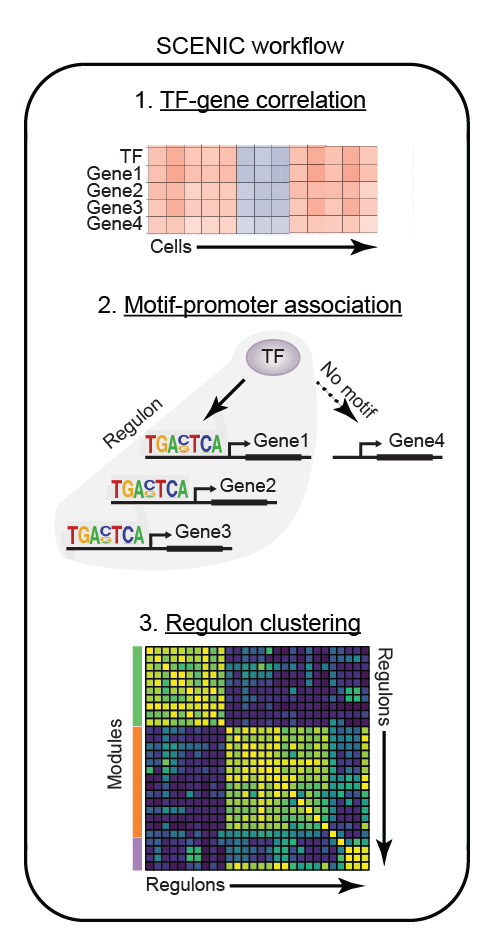
\includegraphics[width=6cm,height=11cm,]{Chapter1/Fig/F3-8-01.png}
% \caption[Inference of gene regulatory networks]{\textbf{\gls{grn} inference using SCENIC.} The SCENIC workflow consists of three steps: identify co-expressed genes with \glspl{tf} (step 1); perform cis-regulatory motif analysis to identify regulons (step 2); evaluate regulon activity in cells and cluster regulons in order to identify coordinated activity of multiple \glspl{tf} (step 3).}
% \label{fig:chp1_grn}
% \end{wrapfigure}

\par One of the widely used computational methods for \gls{grn} inference is SCENIC (single-cell regulatory network inference and clustering) \textbf{\cite{aibar_scenic_2017,van_de_sande_scalable_2020}} which simultaneously constructs \gls{grn} and identifies cell states from \gls{scr} data. SCENIC works by first identifying a set of genes that are co-expressed with a given \gls{tf}, using GENIE3 \textbf{\cite{huynh-thu_inferring_2010}} or GRNBoost2 \textbf{\cite{moerman_grnboost2_2019}} and cis-regulatory \gls{tf} databases. In the second step, SCENIC identifies and filters \gls{tf}-target genes modules based on significant enrichment of motifs using  RCisTarget \textbf{\cite{aibar_scenic_2017,noauthor_rcistarget_nodate}}. These modules are henceforth termed as \textbf{regulons}. These regulons are evaluated in each cell to determine \gls{tf} activation using AUCell \textbf{\cite{aibar_scenic_2017,noauthor_aucell_nodate}}, resulting in activity scores for each cell. Implementations of this \gls{grn} inference workflow exists both in R and Python (\textit{pySCENIC}) \textbf{\cite{kumar_inference_2021}} languages. The recent update, SCENIC+ \textbf{\cite{bravo_gonzalez-blas_scenic_2023}} allows the incorporation of single-cell chromatin accessibility data with motif discovery to infer enhancer-driven \glspl{grn} (eGRNs). In addition to SCENIC+, couple of other tools that leverage single-cell multi-modal inforamtion to infer \glspl{grn} include CellOracle \textbf{\cite{kamimoto_dissecting_2023}} and Pando \textbf{\cite{fleck_inferring_2023}}. 
%The regulons are then scored and evaluated for TF activation in each cell, in a binary fashion (0 = “OFF” and 1 = “ON”),using AUCell , to identify cells or clusters with high subnetwork activity. The result is a list of regulons and their activity scores for all the cells in the data. 


%\clearpage

\subsubsection{Trajectory Inference}
\label{sec:scrna_analysis_grn}
%\colorbox{green}{text clean-up}\\

% \begin{wrapfigure}{r}{0.5\textwidth}
% 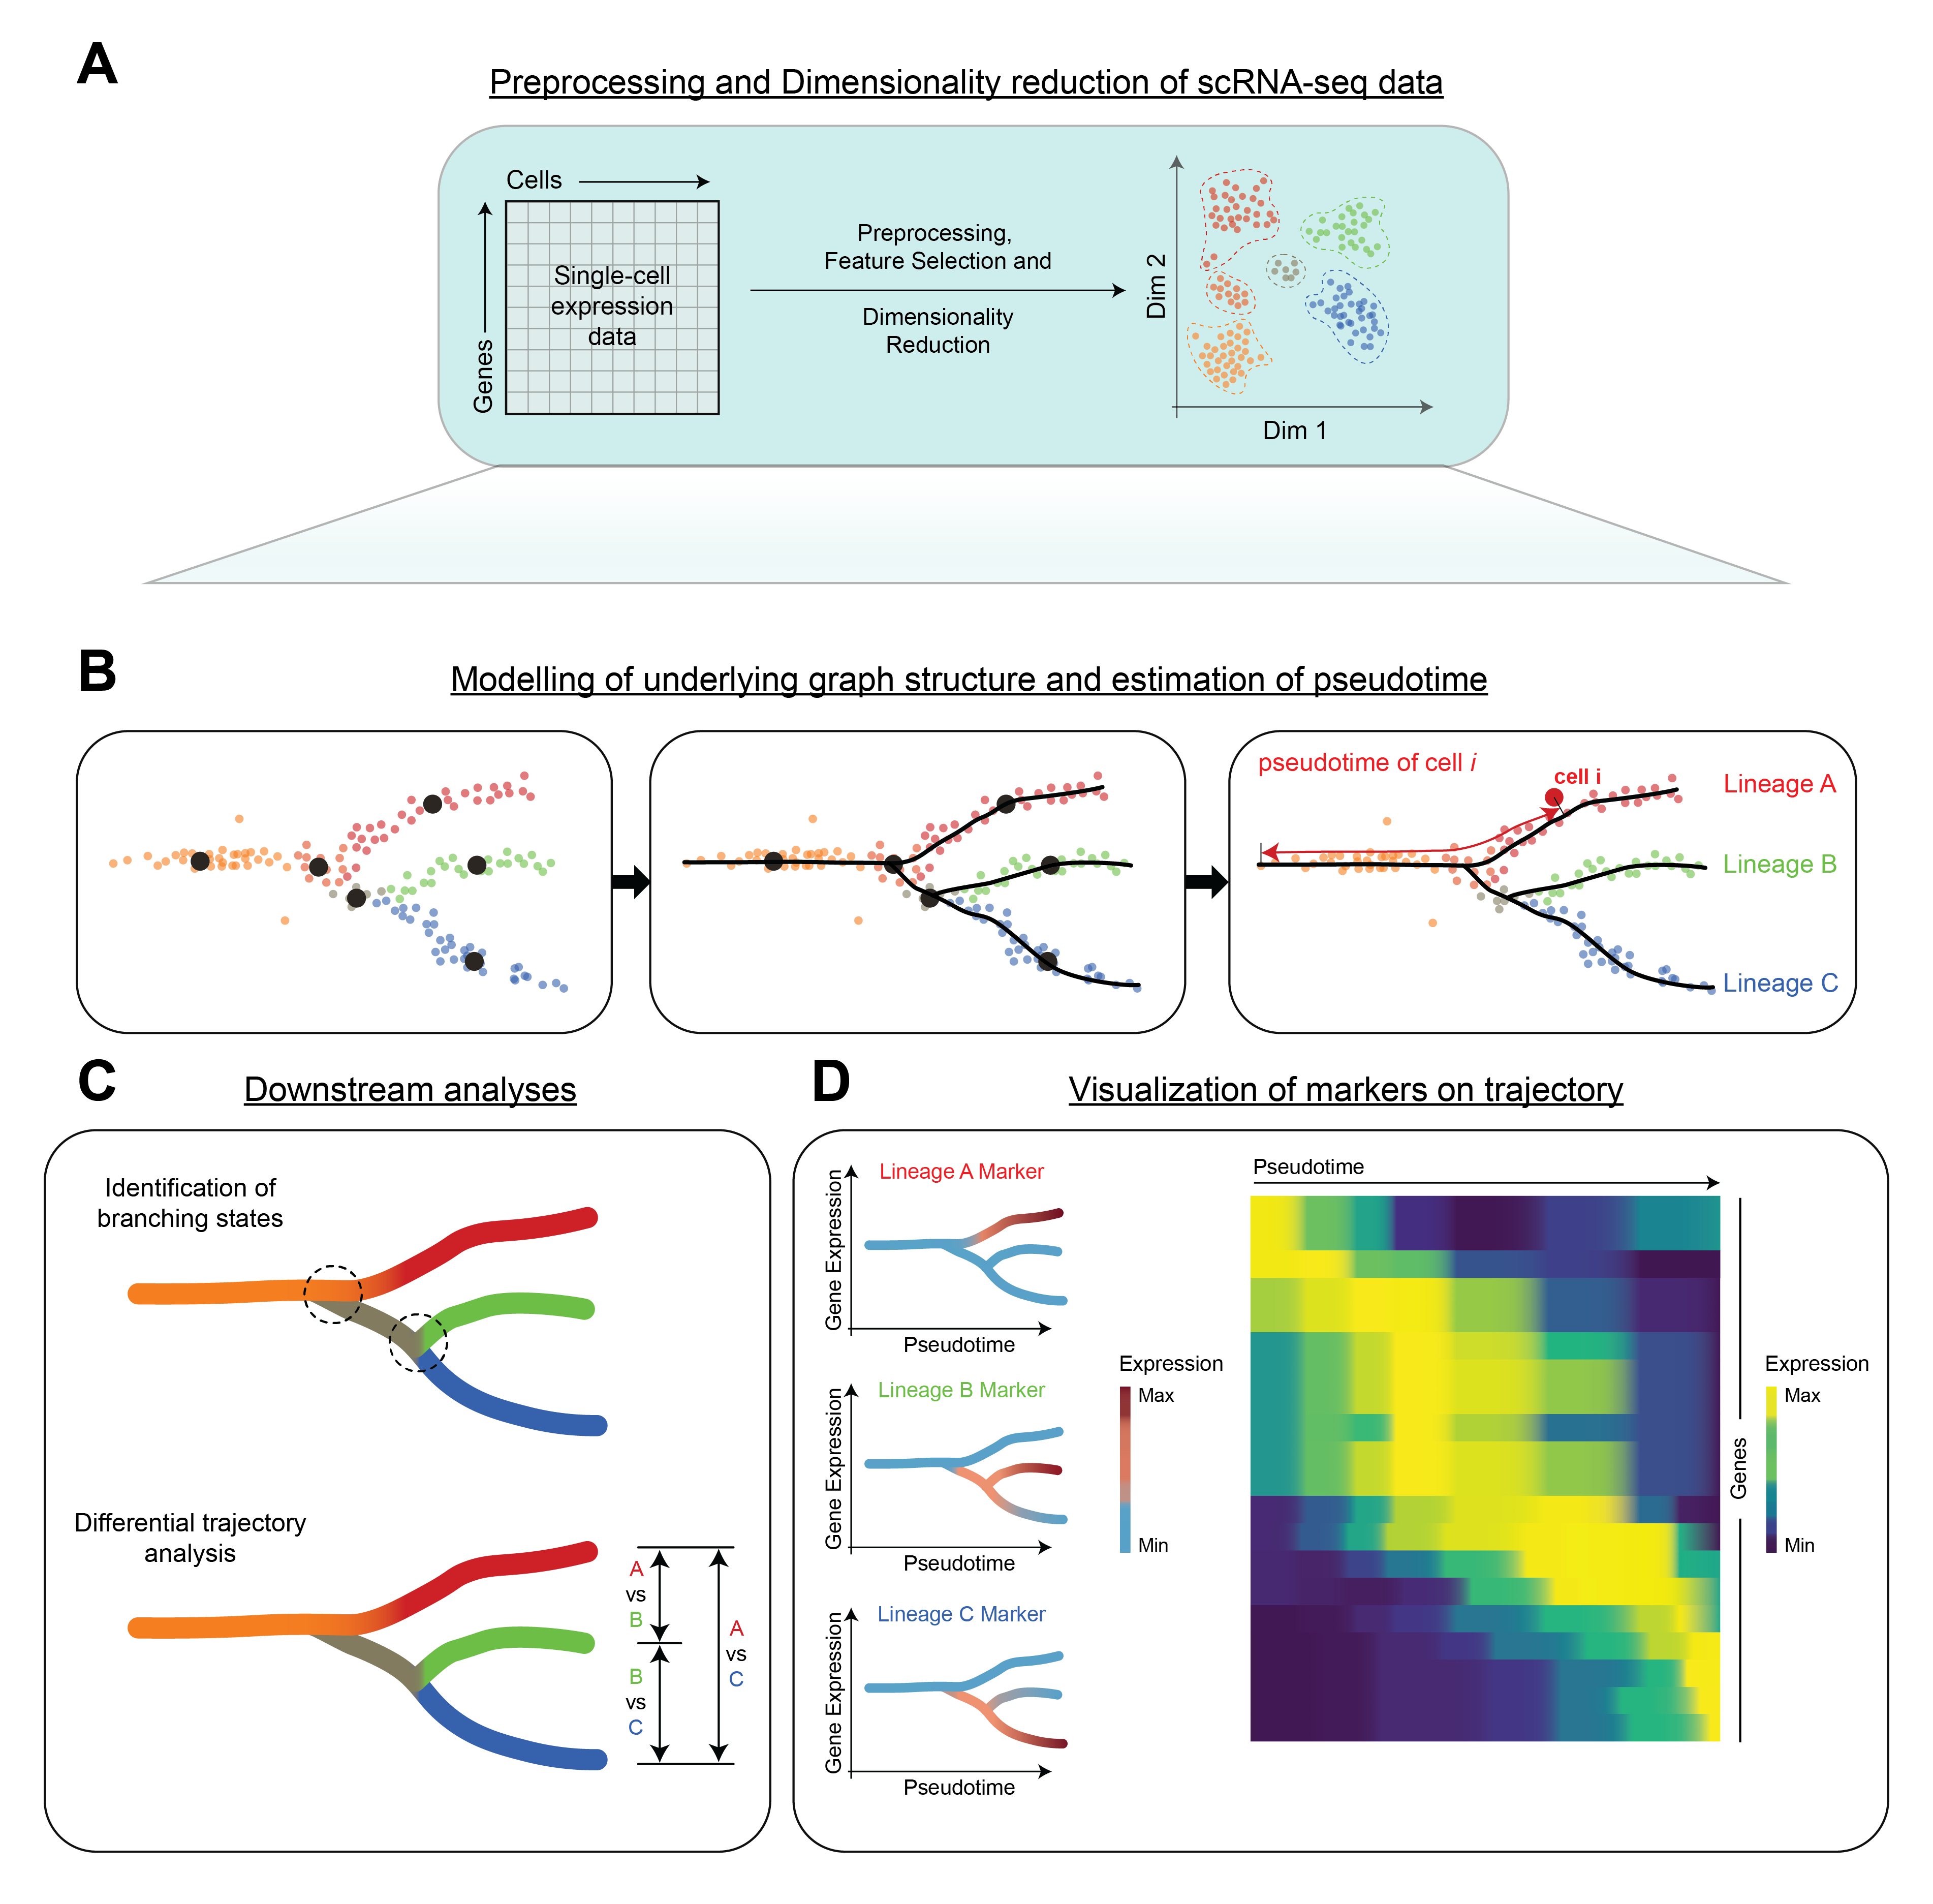
\includegraphics[width=8cm]{Chapter1/Fig/F1-4-01.png}
% \caption[Trajectory inference in scRNA-seq analyis]{\textbf{Trajectory Inference in scRNA-seq analyis} \textbf{(A)} Schematic depicting a typical analysis pipeline for a exemplary scRNA-seq data, visualized in a 2D plot. The data consists of six different hypothetical clusters . \textbf{(B)} Schematic depicting a tree-based TI method applied onto the exemplary scRNA-seq data in panel \textbf{(A)}. Based on the observed hypothetical branching, three hypothetical lineages are determined. \textbf{(C)} Examples of downstream analysis steps that can be performed once a trajectory is inferred on the data. \textbf{(D)} Panel depicting some of the common visualization strategies applied to depict the gene expression changes across trajectories or pseudotime.}
% \label{fig:chp1_trajectory}
% \end{wrapfigure}

\par \gls{scr} data (which are collected at a single interval or time-point) represent only a snapshot of a continuous biological process (\textit{e.g.}, cell differentiation, cell development or cell fate decisions). During this process, cells traverse their cellular states as a result of transient or dynamic gene expression in response to any given stimuli \textbf{\cite{zeng_what_2022}}. However, understanding the continuous cellular processes with \gls{scr} data is challenging, and a key analysis step is linking the cells (or cell-types/states) within or across time-points. The class of methods which model these continuous spectra of cell states and order cells along a trajectory based on their transcriptomic similarity are known as \gls{ti} methods \textbf{(Fig. \ref{fig:chp1_scrna-workflow} D)} \textbf{\cite{ weiler_guide_2022}}. The cells along this pseudotemporal trajectory have progressively changing transcriptome, thereby reconstructing the dynamic gene expression and recapitulating the underlying biological process \textbf{\cite{hou_statistical_2023}}. Each cell is assigned a continuous abstract value, called \textbf{pseudotime}, which represents a cells’ position along this spectrum \textbf{(Fig. \ref{fig:chp1_scrna-workflow} D)}.
\gls{ti} methods are applied to \gls{scr} data in two steps: \textbf{(i)} performing \gls{dr} (using \gls{pca}, ICA, diffusion maps, \gls{tsne} or \gls{umap}) and, \textbf{(ii)} constructing a graph-based trajectory through the reduced-dimensional space. The trajectory itself could be linear, bifurcating or branching, however, complex trajectories such as cycles or disconnected graphs are also possible. This is dependent on the data or biological question being analysed and requires additional prior biological knowledge to aid in the choosing of appropriate \gls{ti} method. Over 150 \gls{ti} tools have emerged \textbf{\cite{noauthor_scrna-tools_nodate,zappia_exploring_2018}}, each with different assumptions, mathematical models, and computational requirements. Monocle v3 \textbf{\cite{cao_single-cell_2019}} and \gls{paga} \textbf{\cite{wolf_paga_2019}} are two of the most popular \gls{ti} methods. A more detailed description of several of these tools along with their advantages and pitfalls can be found elsewhere \textbf{\cite{ding_temporal_2022,deconinck_recent_2021,cannoodt_computational_2016,saelens_comparison_2019}}. A comprehensive benchmarking, along with a practical guideline to assist with the choice of TI method is also available \textbf{\cite{saelens_comparison_2019}}. %\gls{ti} methods have become crucial in studying cellular differentiation and dynamics, and it's advised to verify their trajectories with multiple methods to ensure accuracy and avoid bias.

%TI methods are typically applied on processed, high-quality scRNA-seq data. Therefore, the inherent assumption is that, the data is rid of any noise such as ambient mRNA or empty droplets, doublets or multiplets as well as any low-quality cells. Additionally, accounting for major sources of technical (e.g., sequencing depth) and/or biological variation (e.g., cell-cycle) may be useful to isolate the expected trajectory. TI methods typically consist of two main steps. In the first step, dimensionality reduction (using PCA, ICA or diffusion maps) is performed on the high-dimensional data to convert it into a more simplified representation. In case of a dataset with several thousands of cells, this simplified data can be further projected onto two or three dimensions using tSNE or UMAP (for ease of visualization). In the second step, the graph structure (a trajectory tree) is modelled on this low dimensional manifold of cells. This makes the modelling of the trajectory itself easier in the second step. Therefore, a trajectory is constructed through this reduced space, aiming to identify different cellular states and the trajectory that traverses through them. The trajectory itself could be linear, bifurcating or branching, however, complex trajectories such as cycles or disconnected graphs are also possible. This is dependent on the data or biological question being analysed and requires additional prior biological knowledge to aid in the choosing of appropriate TI method. After this, cells can themselves can be ordered based on their estimated pseudotime values \hyperref[fig1-4]{\textbf{Fig. 1.4}} \\ %\textbf{(Fig. \ref{fig1-4})}.\\\\


%Since 2014, when two computational methods: Monocle and Wanderlust, established the TI field \textbf{\cite{lueckenmalte_d_current_2019}}, over 150 tools have been developed to infer trajectories from single-cell data. The pioneer tool, Monocle \textbf{\cite{trapnell_pseudo-temporal_2014}}, uses ICA for dimensionality reduction and infers a trajectory by constructing a minimal spanning tree (MST). The most recent update (Monocle v3 \textbf{\cite{cao_single-cell_2019}}) involves the use of principal graph algorithm and computing the pseudotime of cells as a geodesic distance from a user-selected ‘root’ or starting cells. Other methods such as partition-based graph abstraction (PAGA) \textbf{\cite{wolf_paga_2019}} construct a knn-graph based representation of cell clusters and allowing for the modelling of more complex trajectories. Overall, these TI methods apply different mathematical models and assumptions, from distance metrics to dimensionality reduction techniques to incorporation of prior knowledge to best capture the underlying biological process. \st{These tools vary in several aspects such as the kind of topology that could be estimated, the dimensionality reduction method employed, the overall modelling approach, the extent of prior biological information required or the computational efficiency of the methods}. Additionally, tools also vary in their ease of use and the available documentation and resources. A more detailed description of several of these tools along with their advantages and pitfalls can be found elsewhere \textbf{\cite{ding_temporal_2022,deconinck_recent_2021,cannoodt_computational_2016,saelens_comparison_2019}}. A comprehensive benchmarking, along with a practical guideline to assist with the choice of TI method is also available \textbf{\cite{saelens_comparison_2019}}.\\\\
%It is clear that TI methods are a powerful feature of downstream scRNA-seq data analysis and therefore have been widely applied to study cell differentiation and development \textbf{\cite{cao_single-cell_2019,sun_time-course_2021,herault_single-cell_2021,li_single-cell_2021,meistermann_integrated_2021,liang_temporal_2022,anderson_single-cell_2023}}, immune responses \textbf{\cite{xu_differential_2020,carpen_single-cell_2022,nguyen_trajectory_2022,luo_multidimensional_2022,xiang_single-cell_2023}}, cellular dynamics and disease progression \textbf{\cite{xin_pseudotime_2018,pang_single-cell_2019,pagliaro_single-cell_2020,bao_pseudotime_2021,dong_single-cell_2021,jansky_single-cell_2021,bazyari_deciphering_2023}}. However, it is important to note that these TI methods work under several general as well as method-specific assumptions. Therefore, a recommended practice is to  confirm the modelled trajectory with alternative methods to avoid method bias and to ensure the robustness of the trajectory present within the data \textbf{\cite{lueckenmalte_d_current_2019}}.
\label{sec:sc_tpi}

\subsubsection{RNA Velocity}
%\colorbox{pink}{missing figure} \colorbox{orange}{incomplete text} \colorbox{red}{missing references}\\
As \gls{scr} data only provides static snapshots of cellular measurements, it is inherently challenging to study cellular dynamics over time. However, this information can be gleaned by inferring the kinetics of \glslink{mrna}{mRNA} life-cycle or splicing dynamics%\footnote{During transcription, DNA is synthesized into precursor messenger RNA (pre-mRNA). Pre-mRNA contains both expressed regions (exons), as well as non-coding regions (introns) which are redundant for translation. Consequently, introns are removed through splicing. This leaves only exons forming mature mRNA. Finally, the process is completed with the eventual degradation of mRNA.}
. By examining the ratio of unspliced pre-\glslink{mrna}{mRNA} to mature (spliced) \glslink{mrna}{mRNA}, the temporal change in \glslink{mrna}{mRNA} can be inferred. This is termed as \textbf{RNA velocity} and represents a powerful computational method in \gls{scr} data analysis to predict the future state of individual cells \textbf{\cite{weiler_guide_2022}}. A velocity vector for each cell can be estimated based on the ratio of unspliced to spliced transcript counts and visualized as a vector field on a low-dimensional embedding such as \gls{umap} \textbf{(Fig. \ref{fig:chp1_scrna-workflow} D)}. The concept of RNA velocity was first implemented as a steady-state model \textbf{\cite{la_manno_rna_2018}} and then extended to a dynamical model \textbf{\cite{bergen_generalizing_2020}}. Recent advances to velocity inference involve the use of deep-learning frameworks \textbf{\cite{li_relay_2024}}, bayesian probabilistic inference \textbf{\cite{qin_pyro-velocity_2022}} or ensemble learning pipeline \textbf{\cite{wang_velo-predictor_2021}}. 
%Several underlying assumptions are made during RNA velocity inference and corresponding methods provide tools such as phase portraits to check for these assumptions.
As an extension to RNA velocity, the obtained velocity fields can be used as input for CellRank \textbf{\cite{lange_cellrank_2022}}, in order to determine cellular fates. Overall, RNA velocity can be used to pinpoint cells undergoing rapid changes and identify critical regulatory genes involved in the transition. Further explanations, summaries and discussion about the usefulness and the pitfalls of RNA velocity analysis can be found here \textbf{\cite{bergen_rna_2021,zheng_pumping_2022}}.

% The two main steps in RNA velocity analysis are:
% \begin{enumerate}
%     \item estimation of the unspliced and spliced transcript counts from the raw data and
%     \item calculation of RNA velocity by computing the ratio of unspliced to spliced transcript counts and estimating a velocity vector for each cell
% \end{enumerate}
% These high-dimensional velocities can then be visualized as a vector field on a low-dimensional embedding such as UMAP or tSNE.\\\\


% The concept of RNA velocity has unlocked new ways of inferring the direction and speed of movement in the transcriptomic space, thereby enabling predictive models of cellular dynamics. 

%\clearpage

\subsubsection{Cell-Cell Interactions}
%\colorbox{pink}{missing figure}\\
% \par Cells, that make up the tissues, constantly coordinate with each other and their microenvironment. This allows cells to maintain homeostasis, respond to internal and external perturbations, thereby allowing the tissue to function properly. In the absence of proper interactions and coordination, disease ensues. 
\par The complex coordination between cells to maintain homeostasis and respond to internal and external perturbations is a result of \glspl{cci} \textbf{\cite{armingol_deciphering_2021}}.  %whereby cells can send or received biochemical and physical signals, that ultimately influence phenotype and function. 
Cells can interact and influence via specific signalling molecules such as ligands (growth factors, chemokines, cytokines), receptors, metabolites, ions, and structural or secreted proteins from the extracellular matrix \textbf{\cite{armingol_deciphering_2021,armingol_diversification_2024}}. %In particular, interactions mediated through ligands from sender cells and the corresponding cognate receptors on receiver cells are also known as \textbf{cell-cell communication (CCC)}, which culminates in altered gene expression \textbf{\cite{armingol_deciphering_2021,armingol_diversification_2024}}. 
It is crucial to understand how cells interact and communicate, in order to shed light on potential mechanisms underlying biological processes such as development and disease progression. The combination of single-cell transcriptomics and high-confidence \gls{lri} databases, has made it possible to infer putative intercellular communications by examining the co-expression of genes corresponding to the \gls{lr} pairs \textbf{(Fig. \ref{fig:chp1_scrna-workflow} D)} \textbf{\cite{wilk_comparative_2023}}. A highly used \gls{cci} prediction tool, CellChat \textbf{\cite{jin_inference_2021}}, is considered a core tool, and models the communication probability value for every \gls{lri} pair using the law of mass action and hill function by using the expression levels of ligands and receptors as proxies for their concentration. In addition, a plethora of computational tools have been developed to infer \glspl{cci} from transcriptomics data. These tools have been reviewed in-depth and extensively bench-marked, and I direct the readers to these publications for further reading \textbf{\cite{armingol_deciphering_2021,armingol_diversification_2024,liu_evaluation_2022,xie_comparison_2023,cheng_review_2023}}.\\

\subsection{Other Modalities}
\label{sec:scrna_modalities}

Besides single-cell transcriptomics, a range of other technologies aims to profile the distinct layers contributing to the overall molecular make-up of a cell. Collectively, these single-cell methodologies enable us to uncover cellular diversity from novel perspectives, offering comprehensive and impartial analyses of individual cells \textbf{\cite{stein_single-cell_2021}}. Some of these modalities are:\\

% % \subsubsection{Single-nuclei RNA sequencing (snRNA-seq)}
% % \colorbox{pink}{missing figure} \colorbox{green}{text clean-up}\\
% % snRNA-seq is an alternative to scRNA-seq and is used to profile gene expression in cells that are difficult to isolate due to their size/fragility such as neurons, adipocytes, epithelial cells and multi-nucleated cells \textbf{\cite{kim_perspectives_2023}}. Instead of profiling the cytoplasmic transcriptome, cell-membrane lysis allows for the capture of nuclear transcriptome, which are then processed with scRNA-seq workflows. snRNA-seq is also less susceptible to perturbations in gene expression during cell isolation. The downstream data analysis pipelines for snRNA-seq are similar to those of scRNA-seq as well. Of note, during gene counting, both exonic and intronic reads are used, as more than 50\% of nuclear RNAs in mouse are typically intronic \textbf{\cite{bakken_single-nucleus_2018}}. \st{As mentioned earlier, capturing a fraction of cell’s total mRNA may lead to an underrepresentation of certain transcripts.} In addition, both snRNA-seq and scRNA-seq may be prone to biases in detecting specific cell-types \textbf{\cite{kim_perspectives_2023,oh_comparison_2022}}  and low sequencing depth resulting in misidentified differentially expressed genes \textbf{\cite{quatredeniers_meta-analysis_2023}}.

% % \subsubsection{Single-cell Genomics}
% % \colorbox{pink}{missing figure} \colorbox{green}{text clean-up}\\

\textbf{Single-cell Genomics: }This modlity, also referred to as single-cell \glslink{dna}{DNA} sequencing is used to interrogate \glslink{dna}{DNA} at the level of individual cells. It enables researchers to better comprehend intercellular variation and heterogeneity by studying single nucleotide variants, copy number variations and microsatellite variations \textbf{\cite{stein_single-cell_2021,luquette_identification_2019,mallory_methods_2020,woodworth_building_2017}}.\\
% As single cells contain only two copies of genomic DNA, several whole genome amplification methods have been developed in order to obtain enough material for subsequent library preparation \textbf{\cite{stein_single-cell_2021,gawad_single-cell_2016,kashima_single-cell_2020}}. \st{In this technology, the genomic DNA is amplified using whole-genome amplification methods146,147. This step is necessary because only two copies of genomic DNA are present in single cells138,147}. Other challenges include isolation techniques, allelic dropout events and variable sequencing depth due to amplification bias which require to be constantly addressed \textbf{\cite{stein_single-cell_2021,gawad_single-cell_2016,kashima_single-cell_2020}}. Despite these challenges, SGP has been extensively used in cancer biology to trace clonal evolution \textbf{\cite{stein_single-cell_2021,kashima_single-cell_2020}}, resolve intra-tumour heterogeneity \textbf{\cite{gawad_single-cell_2016}}, enabled genome assembly of new phyla thereby providing insights into “microbial dark matter” \textbf{\cite{gawad_single-cell_2016}}  and and reconstruct cell lineages in tumour tissues, characterize rare cell types \textbf{\cite{stein_single-cell_2021,liu_current_2017}}. The further development of robust and scalable technologies associated with SCG and improvements in genome coverage, throughput and integration with other -omics approaches will enable more comprehensive analyses of cellular heterogeneity providing insights into cancer evolution, developmental biology and genetic disorders.

% % \subsubsection{Single-cell Epigenomics}
% % \colorbox{pink}{missing figure} \colorbox{orange}{incomplete text}\\
\textbf{Single-cell Epigenomics: }In recent years, there has been rapid development in single-cell methods to assay epigenetic features such as \glslink{dna}{DNA} methylation with \glslink{scbs}{scBS-seq} \textbf{\cite{smallwood_single-cell_2014}}, %, scWGBS \textbf{\cite{farlik_single-cell_2015}}, scRRBS \textbf{\cite{guo_single-cell_2013}} ), 
 histone modifications with \glslink{chip}{scChIP-seq} \textbf{\cite{grosselin_high-throughput_2019}}, %scCUT\&Tag \textbf{\cite{kaya-okur_cuttag_2019,wu_single-cell_2021}} ), 
 %%The advent of single-cell epigenomic technologies have enabled researchers to gain unprecedented resolution and insights into cellular diversity, modes of gene regulation, TF dynamics, and 3D genome organization at single-cell level. 
 chromatin accessibility with \glslink{scatac}{scATAC-seq} \textbf{\cite{chen_rapid_2018,xu_plate-based_2021,buenrostro_single-cell_2015,satpathy_massively_2019}} and chromosome conformation \textbf{\cite{stevens_3d_2017,dekker_capturing_2002}}. 
 %which the researchers have extensively used to survey the epigenetic landscape of cells. For example, DNA methylation data has been used to predict biological age from ’epigenetic clocks’ \textbf{\cite{horvath_dna_2018}}. On the other hand, patterns of chromatin accessibility can provide significant understanding of biological function by identifying key responsive TFs across variable TF binding between cells \textbf{\cite{buenrostro_single-cell_2015}}. 
 Moreover, single-cell chromosome conformation studies combined with co-accessibility patterns can provide unprecedented detail of 3D genome organization \textbf{\cite{mazan-mamczarz_single-cell_2022}}.\\
% % These epigenetic modifications play a crucial role in regulating gene expression and cellular identity and single-cell epigenomics data are a valuable addition to transcriptomic and proteomic profiles of cells and further enrich our understanding of multi-layered regulatory networks that dictate cellular fate and responses. The analysis of single-cell epigenomics data presents unique challenges. Extensive reviews providing a comprehensive overview of single-cell epigenomics, associated data-analysis strategies as well discussions on current outlook and futures perspective are referred here \textbf{\cite{preissl_characterizing_2023}}.


% % \subsubsection{Single-cell Proteomics}
% % \colorbox{pink}{missing figure} \colorbox{red}{missing references} \colorbox{orange}{incomplete text}\\
\textbf{Single-cell Proteomics:}
% % Proteins are the most important functional macromolecules within cells, carrying out a vast array of tasks such as regulation of gene expression, catalysing metabolic reactions, ferrying molecules and controlling signalling \textbf{\cite{labib_single-cell_2020,proteomics}}. Therefore, surveying the protein landscape of a cell at single-cell resolution is essential to capturing the full functional heterogeneity of the cell and discovering new biological regulators.\\\\
% % Single-cell proteomics (SCP) 
This modality is an emerging field, aiming to generate hypothesis-free protein expression from individual cells \textbf{\cite{ctortecka_rise_2021,}}. %In addition to the high-resolution proteome data, 
Single-cell proteomics provides insights into post-translational modifications, which is completely inaccessible at the transcriptomic level \textbf{\cite{labib_single-cell_2020,ctortecka_rise_2021,petrosius_recent_2022}}, and allows for the %Further, the availability of SCP data facilitates the 
characterization of cellular processes and states independent of the corresponding \glslink{mrna}{mRNA} levels.%, with accumulating evidence pointing to a discordance between the two for most genes, at both, population and single-cell \textbf{\cite{ctortecka_rise_2021,petrosius_recent_2022,bennett_single-cell_2023}}. 
 Several strategies have been developed to study the proteome at single-cell resolution: mass-spectrometry based methods \textbf{\cite{petrosius_recent_2022,budnik_scope-ms_2018,zhu_nanodroplet_2018}}; antibody-based methods; imaging-based methods to provide spatial context \textbf{\cite{paul_imaging_2021,chang_imaging_2017,keren_mibi-tof_2019}}; and single-molecule sequencing methods \textbf{\cite{alfaro_emerging_2021}}.\\    %\hl{......}\\\\
% % However, comprehensive analysis of proteins at single-cell resolution has remained a challenge. Although, still in a more nascent state compared to single-cell genomic or transcriptomic technologies, recent advancements in mass spectrometry (MS)-based proteomics such as instrumentation, sample preparation workflows, chromatography and ion mobility have facilitated the progress of this field \textbf{\cite{ctortecka_rise_2021,petrosius_recent_2022}}.\\\\

% \subsubsection{Single-cell multi-omics}
% \colorbox{pink}{missing figure}
\textbf{Single-cell multi\textit{-omics}: }The integration of data across multiple modalities offers finer insights about individual cells and provides complementary information between layers due to the inherent differences between them and improve our ability to identify cell-types and cell-states \textbf{\cite{flynn_single-cell_2023}}. This has prompted the development of single-cell multi\textit{-omics} technologies which allow for simultaneous profiling of genome, epigenome, transcriptome, proteome and other modalities. Several multi\textit{-omics} methods utilize the transcriptome profiling as an anchor to facilitate downstream integration of the several layers \textbf{\cite{baysoy_technological_2023}}. The transcriptome profiling can be combined with genomics (\glslink{gandt}{G\&T-seq}) \textbf{\cite{macaulay_gt-seq_2015}}, epigenome (\glslink{mandt}{scM\&T-seq}) \textbf{\cite{angermueller_parallel_2016}}, proteomics (\glslink{cite}{CITE-seq}) \textbf{\cite{stoeckius_simultaneous_2017}} or other modalities \textbf{\cite{dixit_perturb-seq_2016,singh_high-throughput_2019}}, offering a multi-layered approach to single-cell analysis.\\
% \par The various single-cell ‘single-omics’ methods have generated a vast array of data from individual modalities allowing for the examination of cellular properties and the dissection of the mechanisms of gene regulation at a single-cell level. 
%While single modalities provide important insights, 
 %scNMT-seq \textbf{\cite{clark_scnmt-seq_2018}}),

%information about the interaction between the various layers for any given cell-type or cell-state. In addition, multi-modal analyses can provide complementary information between layers due to the inherent differences between them and improve our ability to identify cell-types and cell-states \textbf{\cite{flynn_single-cell_2023}}.%\st{Multi-omics analyses has been applied on tumours at a bulk level and provided a comprehensive understanding of cellular processes through integration of data on mutations, mRNA, proteins and metabolites} \textbf{\cite{lee_single-cell_2020}}.
% \\
% \begin{figure}[t]
%     \centering
%     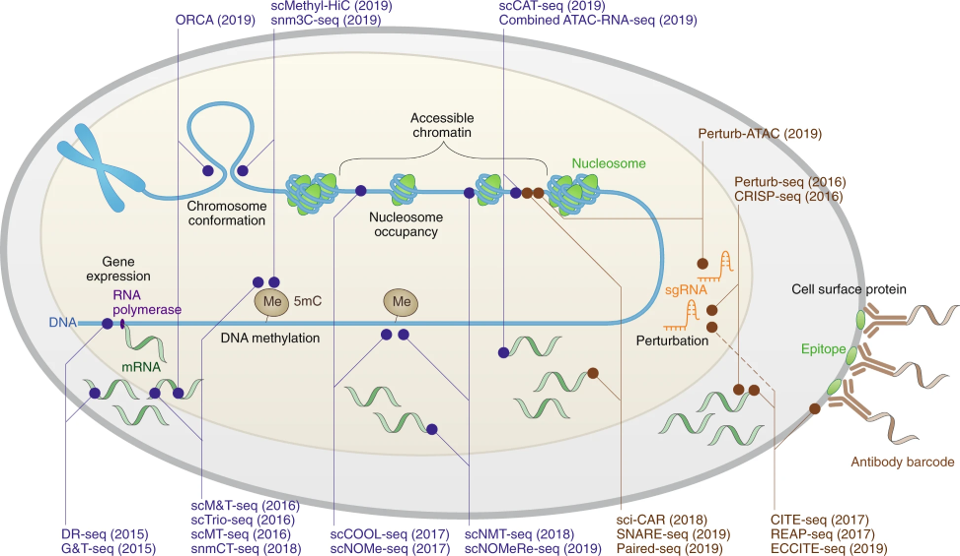
\includegraphics[width=\linewidth]{Chapter1/Fig/F1-7.png}
%     \caption[Overview of single-cell multi\textit{-omics} methods]{\textbf{Methods for single-cell multi-omics analysis.} Illustration depicting several methods to simultaneously profile genome, epigenome, transcriptome and proteome of individual cells. Low-throughput methods are highlighted in blue whereas highly scalable methods for analysis are highlighted in brown. This illustration is taken from \textbf{\cite{}}. \textit{Reproduced with permission from Springer Nature.}}
%     \label{fig:enter-label}
% \end{figure}

%Further, single-cell multi-omics technologies have seen continuous improvements in multiplexing, throughput, resolution and accuracy. 
 %Alongside the development of these technologies, computational strategies to deal with the challenges of combining diverse datasets from various omics layers have also advanced significantly, with current methods employing regression or association techniques, unsupervised integration, data-ensemble, model-ensemble \textbf{\cite{vahabi_unsupervised_2022, stanojevic_computational_2022}} or deep-learning algorithms \textbf{\cite{baysoy_technological_2023,athaya_multimodal_2023}}. The complexity and high-dimensionality of single-cell multi-omics data presents several challenges for computational approaches such as a lack of harmonized data format across modalities, the non-alignment of modalities in case of unpaired datasets, the multiplication of technical noise across several layers, all of which require continuous development and refinement of these methods. Ultimately, single-cell multi-omics technologies offer immense potential in elucidating complex biological processes in health and diseases by simultaneously capturing complementary information from various biological layers. For further reading, interested readers can refer to several reviews summarizing the various technologies and their applications, computational tools to analyze multi-modal data as well as discussions on current challengers and future perspectives in this field \textbf{\cite{flynn_single-cell_2023,lee_single-cell_2020,baysoy_technological_2023, miao_multi-omics_2021, dimitriu_single-cell_2022}}.





% \subsubsection{Spatial Technologies}
% \colorbox{pink}{missing figure} \colorbox{red}{missing references} \colorbox{orange}{incomplete text}\\
\textbf{Spatial Technologies: } %While the \textit{-omics} technology have revolutionized our ability to characterize cells and led to the identification of novel cell-types, cell states and a better understanding of mechanisms in health and diseases, 
The inability to apply single-cell methods \textit{-omics} methods \textit{in-situ} results in loss of spatial information. Spatial technologies for single-cell \textit{-omics} studies have emerged as powerful tools to enhance our understanding of cellular heterogeneity, complex tissue organization and the dynamic interplay of cells within their micro-environments. A notable example is the emerging field of \gls{st}, which enables the simultaneous assessment of gene expression and visualization of \glslink{mrna}{mRNA} distribution in tissue sections \textbf{\cite{moses_museum_2022,tian_expanding_2023}}.\\ %In the past decade, several high-throughput technologies to quantify gene expression in space and corresponding computational methods have been applied to elucidate the cell-type composition of several tissues, the cellular interactions underlying spatial patterns and molecular interactions at spatial proximities in cases of tumors, immune infiltrates and development. This field has been the subject of many extensive reviews and I direct the readers to extensive reviews for detailed comparisons of different technologies in ST, their applications and future advancements \textbf{\cite{rao_exploring_2021,moses_museum_2022,duan_spatially_2022,tian_expanding_2023,cheng_spatially_2023}}


% %\subsubsection{Single-cell Metabolomics}


% % \\\\
% % In summary, . These techniques and their corresponding computational methods require improvement and benchmarking in order to enhance their accuracy, scalability, and usability, ultimately empowering researchers to gain deeper insights into cellular heterogeneity, regulatory networks, and disease mechanisms. 




% In \textbf{\hyperref[sec:suppnote3]{Supplementary Note 3}}, I have briefly described and summarized CellChat \textbf{\cite{jin_inference_2021}}, a computational tool, designed to infer CCIs from scRNA-seq data. CellChat is considered as a ‘core’ tool	which established a set of methods and is widely used by the scRNA-seq community. 

% \begin{figure}[H]
%     \centering
%     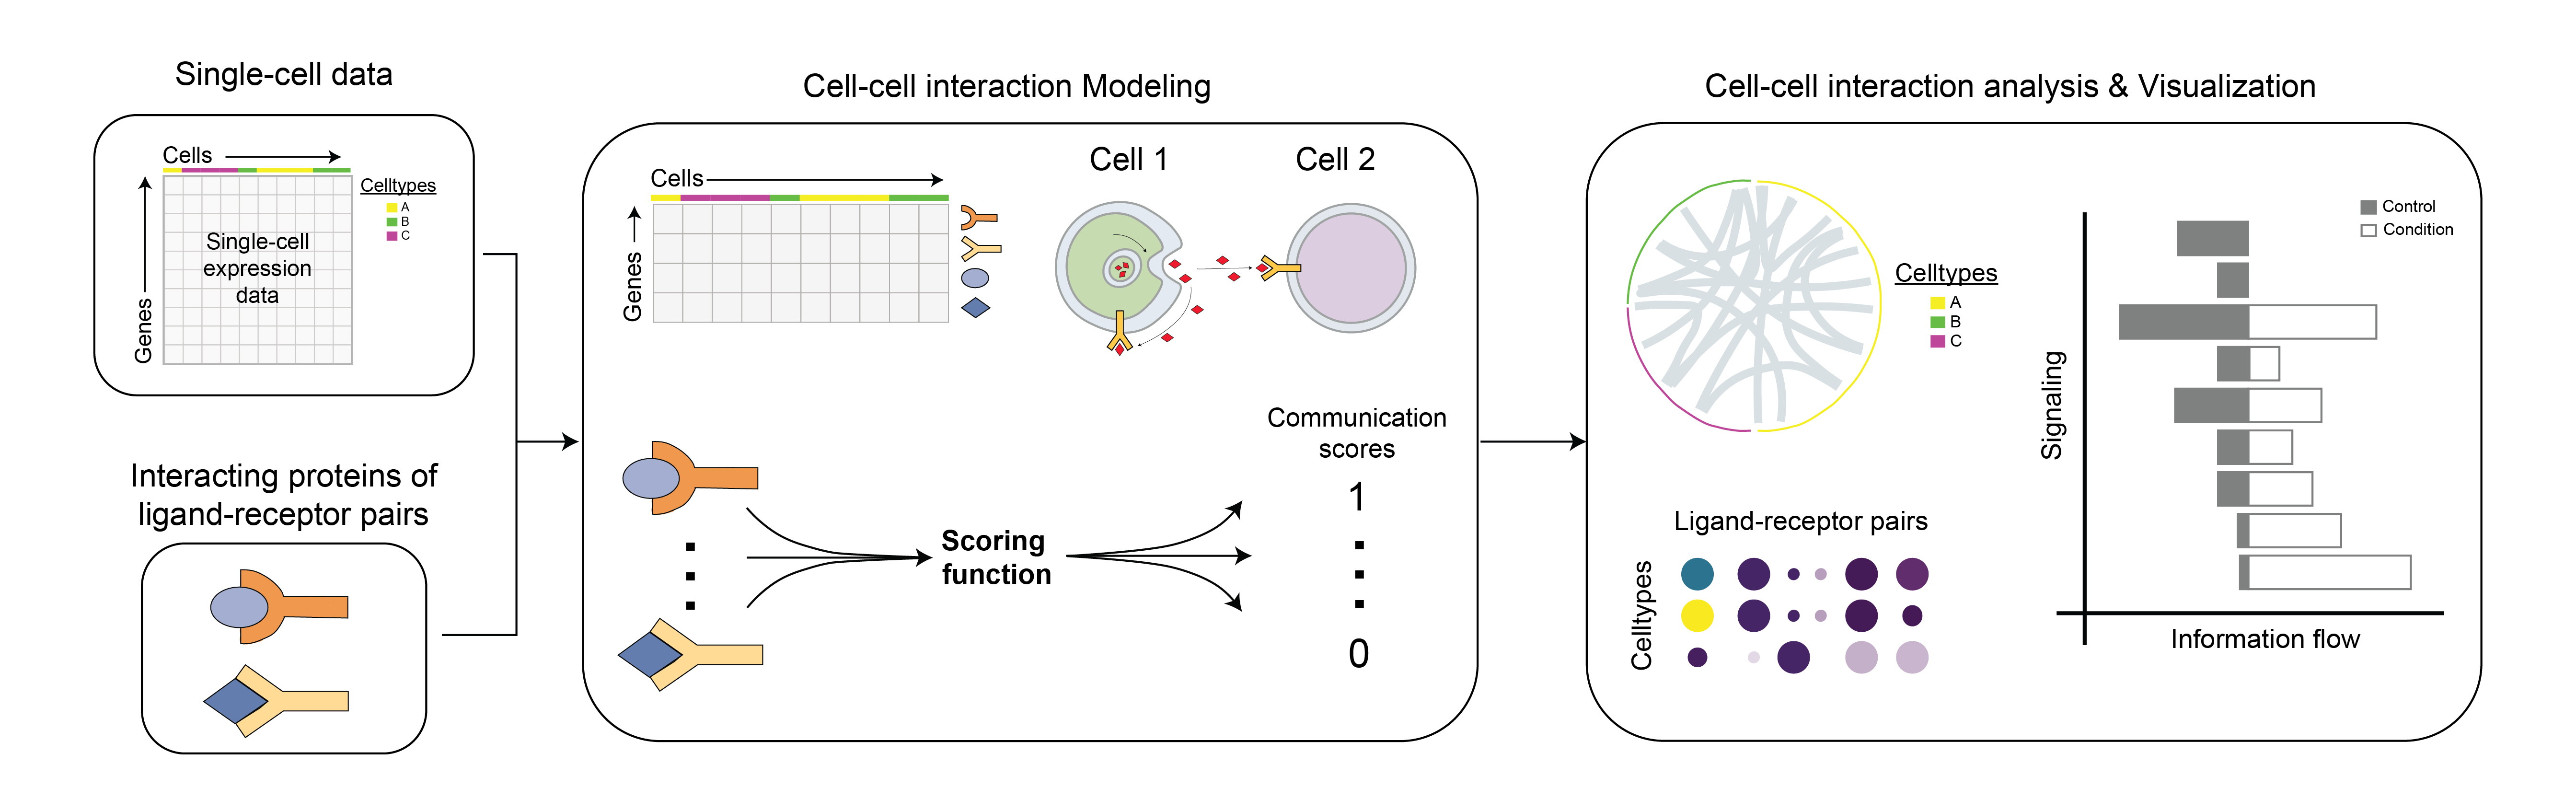
\includegraphics[width=\linewidth]{Chapter1/Fig/F1-6-01.png}
%     \caption[Inference of Cell-Cell interactions]{\textbf{Analysis workflow for inferring cell-cell interactions from scRNA-seq data.} Using curated interactions from ligand-receptor databases, the single-cell gene expression data is filtered to genes associated with the interactions. The expression levels of the genes are used to compute communication scores for every ligand-receptor pair using a scoring function. The communications scores can be represented via various visualizations in order to  further facilitate inference about signaling events between cell-types in the dataset.}
%     \label{fig:chp1_cell-cell}
% \end{figure}

% \newpage

\textbf{Adaptive immune receptor repertoire profiling: }This involves analyzing the diversity of immune receptor sequences such as \glslink{tcr}{TCRs} and \glslink{bcr}{BCRs} at single-cell level. Commercial technologies like the 10x Chromium Single Cell Immune Profiling and BD Rhapsody \glslink{tcr}{TCR}/\glslink{bcr}{BCR} multi\textit{-omic} assays are used for this purpose \textbf{\cite{heumos_best_2023}}. 

\subsection{Single-cell \textit{-omics} in pancreas}
\label{sec:single-cell_pancreas}
%\colorbox{green}{text cleanup}\\
The rapid growth and development of single-cell transcriptomics and other \textit{–omics} assays have greatly advanced our understanding of pancreatic physiology, including development, cellular heterogeneity (including rare cell-types) and disease mechanisms. For a greater overview of findings from multiple studies in this space, the readers can refer here \textbf{\cite{wang_single-cell_2019,avrahami_beta_2017,carrano_interrogating_2017}}. A major outcome from the application of \gls{scr} is the refinement of cell-type specific gene signatures, which includes identifying rare ghrelin-producing $\epsilon$-cells and revealing heterogeneity of $\beta$-cells within islets with sub-types or cell states that exhibit differential markers for \glslink{er}{ER} stress and oxidative response \textbf{\cite{segerstolpe_single-cell_2016,muraro_single-cell_2016}}.\\
% A major outcome from the application of \gls{scr} is the refinement of cell-type specific gene signatures, including the identification of rare ghrelin-producing $\epsilon$-cells in the human pancreas \textbf{\cite{segerstolpe_single-cell_2016}}. Several \gls{scr} studies have identified heterogeneity of $\beta$-cells within islets, with subtypes \textbf{\cite{segerstolpe_single-cell_2016}} or cell states exhibiting differential markers for \glslink{er}{ER} stress and oxidative response \textbf{\cite{muraro_single-cell_2016}}.\\% as well as groups with expression of maturation markers.\\
\par Further \gls{scr} research has mapped both endocrine and exocrine pancreatic lineages, uncovering developmental trajectories and the regulatory mechanisms of intermediate progenitor cells \textbf{\cite{yu_defining_2019}}. A more recent \gls{scr} and \glslink{scatac}{scATAC-seq} study of first trimester human embryonic pancreatic tissues identified differential gene expression between dorsal and ventral multipotent progenitor cells, and identified endocrine progenitor sub-clusters with different differentiation potentials. The authors also noted distinct gene expression patterns between human and mouse developmental trajectories \textbf{\cite{ma_deciphering_2023}}. A spatio-temporal study characterized islet formation as budding peninsulas rather than mere aggregations, showing $\alpha$-cells developing first in the outer layer followed by $\beta$-cells beneath, thereby reflecting eventual mature islet architecture \textbf{\cite{sharon_peninsular_2019}}. An integrated \gls{scr} and \gls{st} study of fetal human pancreas revealed distinct spatio-temporal gene cascades and multiple lineage dynamics within the pancreas contributing to the exocrine acinar state \textbf{\cite{olaniru_single-cell_2023}}.\\

% distinct spatio-temporal gene cascades. In addition, spatial differentiation trajectories co-localized Schwann cells with endocrine progenitors, and also identified heterogeneity and multiple lineage dynamics within the pancreas which contributed to the exocrine acinar state \textbf{\cite{olaniru_single-cell_2023}}.

% Integrating scRNA-seq with spatial transcriptomics has revealed distinct spatio-temporal gene cascades and multiple lineage dynamics within the pancreas, contributing to our understanding of pancreatic organogenesis and disease progression [378]
%In recent years, researchers have utilized \gls{scr} to investigate both endocrine and exocrine pancreatic lineages, developmental trajectories and regulatory mechanisms of intermediate progenitor populations along the developmental pathway. One such study identified multiple stages of endocrine precursor cell differentiation before the allocation of islet lineage in several reporter mouse strains \textbf{\cite{yu_defining_2019}}. A more recent \gls{scr} and \glslink{scatac}{scATAC-seq} study of first trimester human embryonic pancreatic tissues identified differential gene expression between dorsal and ventral multipotent progenitor cells, and identified endocrine progenitor sub-clusters with different differentiation potentials. The authors also noted distinct gene expression patterns between human and mouse developmental trajectories \textbf{\cite{ma_deciphering_2023}}. In another single-cell spatio-temporal study, the authors depicted that the islet morphology and endocrine differentiation are closely related and that the islets form as budding `peninsulas' as opposed to aggregation of dispersed cells \textbf{\cite{sharon_peninsular_2019}}. In this peninsular morphology, $\alpha$-cells develop first in the outer layer and $\beta$-cells develop later, beneath them, thereby reflecting eventual mature islet architecture. Another study involving human fetal pancreas in second trimester identified an uncommitted multipotent progenitor cells directing self-renewal and pancreatic organogenesis \textbf{\cite{villani_sox9ptf1a_2019}}. A comparative study between transcriptomes and chromatin profiles of endocrine cells during \textit{in vitro} differentiation and childhood and adult pancreas, described spatio-temporal gene regulatory relationships between \glspl{tf} and observed insufficient activation of signal-dependent \glspl{tf} during \textit{in vitro} $\beta$-cell maturation \textbf{\cite{zhu_understanding_2023}}. By mapping individual $\beta$-cells from mouse pancreata along an `inferred' maturation trajectory, two studies identified signatures of immature $\beta$-cells \textbf{\cite{qiu_deciphering_2017,zeng_pseudotemporal_2017}}. The pseudotemporal analysis of postpartum $\beta$-cell development depicted a crucial role for reactive oxygen species and amino acids, with the algorithm proclaiming significant changes in $\beta$-cell metabolism during early postnatal period. A similar analysis of $\beta$-cells from human non-diabetic deceased donors suggested that $\beta$-cells are separated by states of high insulin biosynthesis followed by recovery from the ensuing \glslink{er}{ER} stress by activation of \gls{upr} pathway \textbf{\cite{xin_pseudotime_2018}}.  Interestingly, the algorithm revealed a branching pattern among the $\beta$-cell states indicating potential $\beta$-cell sub-populations, similar to previous studies.\\
%As discussed in the earlier section, the two major types of diabetes are associated with autoimmune destruction (T1DM) of β-cells or with the dysfunction and loss (T2DM) of β-cells, leading to insulin resistance. Therefore, 
\par A major goal of diabetes research is the replenishment of missing or abnormal $\beta$-cells. A single-cell \glslink{mrna}{mRNA} and \glslink{crispr}{CRISPR} screen study identified several genes at obesity and \gls{t2d} loci associated with $\beta$-cells \textbf{\cite{fang_single-cell_2019}}. %several genes at obesity loci and \gls{t2d} loci associated with $\beta$-cells. Obesity is a major risk factor in the development of \gls{t2d} and the study identified various genetic commonalities between the two diseases \textbf{\cite{fang_single-cell_2019}}. 
In another study, the authors utilized \glslink{snatac}{snATAC-seq} assay to uncover heterogeneity in regulatory programs of $\beta$-cell states and that the genetic risk of \gls{t2d} is likely mediated through a state of high insulin production and other functional states related to stress and signaling responses \textbf{\cite{chiou_single-cell_2021}}. %Moreover, the study also implicated other endocrine cell types, particularly $\delta$-cells, with the genetic risk of \gls{t2d}.
Comparative analysis of single-cell transcriptomic data from \gls{t2d} donors with machine-learning classifiers revealed that $\beta$-cells typically manage insulin production under low stress but display dysfunctional responses under high stress conditions, with oxidative stress playing a crucial role in influencing \textit{insulin} gene expression \textbf{\cite{ma_single-cell_2018}}.\\ 
\par \gls{scr} has been extensively applied to the study of \gls{pdac}, which is a complex disease and has one of the lowest 5-year survival rate of all tumor entities. A recent review highlighted the multitude of biological insights into heterogeneity, plasticity and response to therapy. The review also outlines that future efforts will focus on integrating \gls{scr} with \gls{st} and advanced screening techniques to better understand the spatial organization, genetic vulnerabilities, and resistance mechanisms in \gls{pdac}, thereby advancing subtype-specific treatments and targeting strategies \textbf{\cite{barthel_single-cell_2023}}.
% A comparative study of three single-cell transcriptomic datasets of \gls{t2d} donors using machine-learning classifiers found that, in \gls{t2d}, $\beta$-cells normally express insulin under low cellular stress and exhibit abnormal functionality upon high stress conditions \textbf{\cite{ma_single-cell_2018}}. In addition, correlation analysis depicted that oxidative stress could represent a crucial factor in influencing insulin expression in \gls{t2d} patients and that expression is also individual-specific.\\ % A recent review summarized that the exocrine pancreas's depicts greater-than-expected epithelial heterogeneity under normal conditions; pancreatic acinar cells show significant plasticity that can influence disease progression through transdifferentiation during injury or oncogenesis. The review also emphasizes how advanced techniques such as scRNA-seq and spatial profiling are crucial in tracing cellular and molecular changes from metaplasia to cancer, shedding light on resistance mechanisms and identifying potential therapeutic targets \textbf{\cite{cephas_it_2023}}.



%\clearpage


% ***************************************************************
%************************ %Sixth Section %****************************************************************
\section{Imaging Mass Cytometry}  %Section - 1.6
\label{sec:IMC}


The organization and interaction of cells within any given tissue is crucial to understand how biological processes occur in health and diseases. Tissue architecture can therefore reveal the mechanisms of disease progression, \textit{e.g.}, how cancer cells can invade surrounding tissues or how immune cells infiltrate and organize in response to infection or injury \textbf{\cite{veenstra_research_2021}}. Traditional staining and imaging techniques such as \glslink{hande}{H\&E} staining \textbf{\cite{titford_progress_2009}}, \glslink{ihc}{IHC} \textbf{\cite{ortiz_hidalgo_immunohistochemistry_2022}}, and \glslink{if}{IF} \textbf{\cite{odell_immunofluorescence_2013}} have been routinely used for histopathology, and have been instrumental in the advancement of cellular biology. However, these techniques have inherent limitations with multiplexing, quantification, spatial resolution, spectral overlap or throughput, thereby hindering in-depth characterization or phenotyping of tissues \textbf{\cite{veenstra_research_2021,leroux_imaging_2021}}. As a result, a highly multiplexed histology technique capable of assessing many markers at the same time, applicable to frequently obtained tissues, with single-cell resolution and high throughput was required.

\begin{figure}[H]
    \centering
    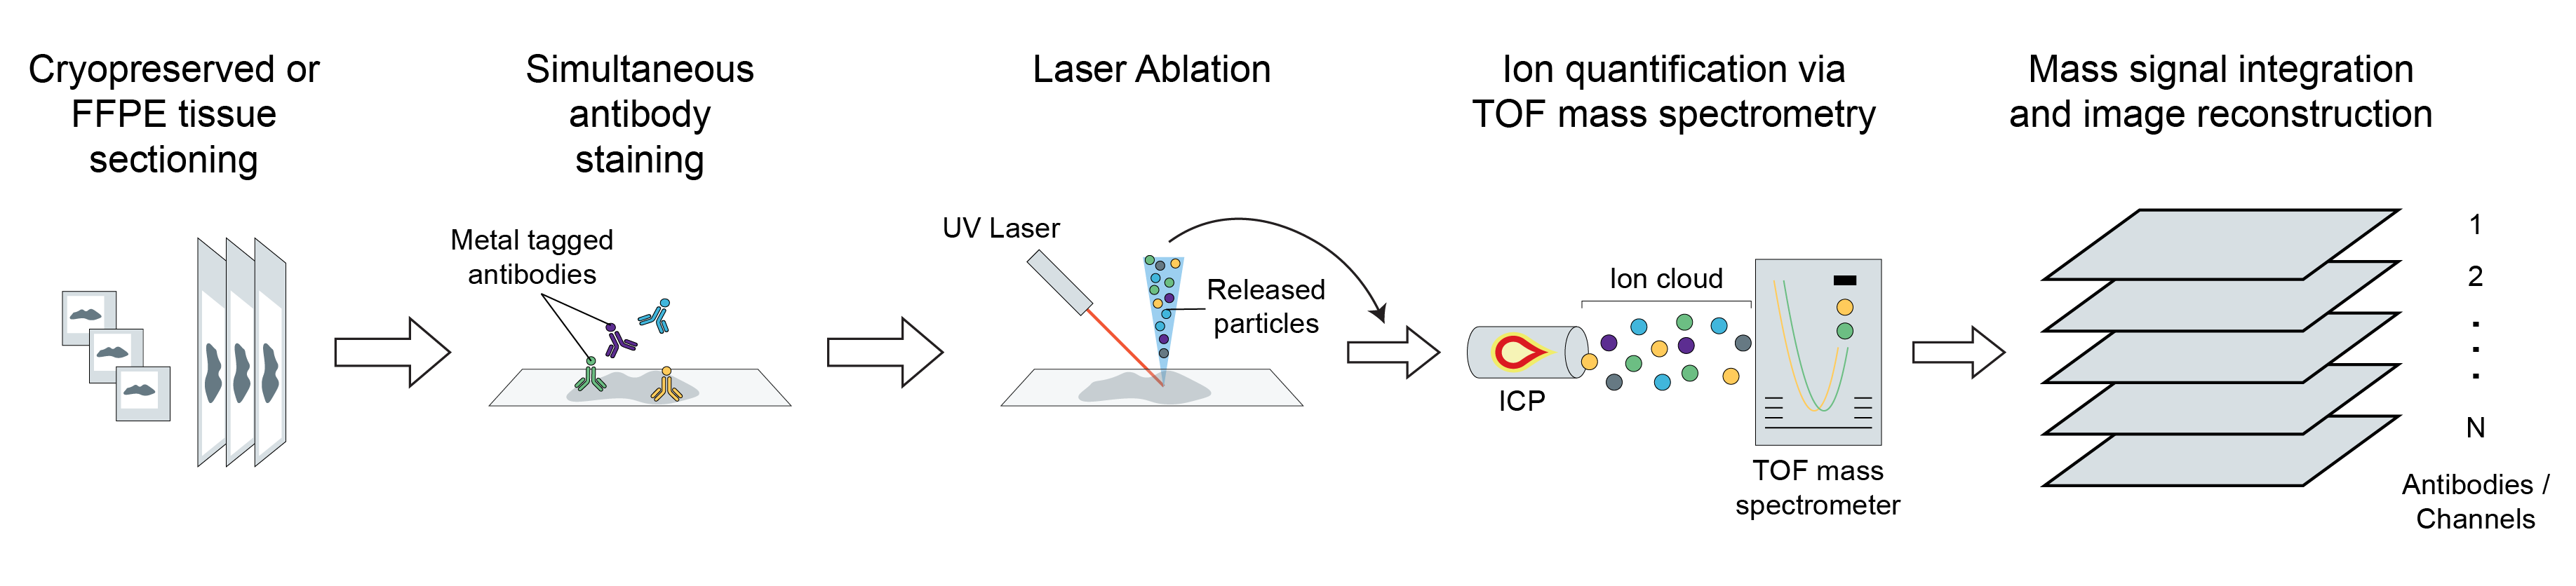
\includegraphics[width=\linewidth]{Chapter1/Fig/F1-12-01.png}
    \caption[Overview of Imaging Mass Cytometry workflow]{\textbf{High-dimensional imaging analysis of tissue sections with \glslink{imc}{IMC}.} Tissue sections from cryopreserved or \glslink{ffpe}{FFPE} samples are stained with heavy metal-tagged antibodies simultaneously. The stained sections are placed in the \glslink{imc}{IMC} analyzer wherein a laser ablates the tissue pixel-by-pixel, releasing particles which are ionized and quantified by a mass spectrometer. Based on ion cloud composition, an image of the ablated area is created for each antibody/channel. Abbreviations: FFPE, formalin-fixed paraffin embedded; ICP, inductively coupled plasma; TOF, time-of-flight. \textit{This image is adapted from }\textbf{\cite{damond_map_2019,hartmann_immune_2020}}. \textit{Reproduced with permission from Springer Nature.}}
    \label{fig:chp1_imc_workflow}
\end{figure}

\par \gls{imc} represents a significant advancement in the field of \gls{cytof}, by combining the fluorescence-based imaging techniques with laser ablation and detection by mass cytometry to generate multiplexed images \textbf{\cite{veenstra_research_2021,chang_imaging_2017}}. In brief, tissue sections (either frozen or \glslink{ffpe}{FFPE}) are stained with a user-determined panel of probes conjugated with stable metal isotopes. The use of non-biological metal isotopes mainly belonging to the lanthanide series nearly eliminates tissue background signals. The stained sections are then ablated by a focused laser beam with 1\textmu m spot size. The laser ablation releases plumes of ions which are carried by an inert gas to the coupled mass spectrometer to be detected and analysed. This allows for tracing back the signals for multiple probes from each spot back to the respective coordinates in the scanned area. The mass resolution of the mass spectrometer enables low spectral overlap \textbf{(Fig. \ref{fig:chp1_imc_workflow})}
\textbf{\cite{veenstra_research_2021,chang_imaging_2017}}.\\


%\clearpage

\par After image acquisition, conversion of the raw \gls{imc} images enables the extraction of multi-modal, multi-region, multi-channel information. Individual acquisitions can be extracted as \glslink{tiff}{TIFF} and \glslink{otiff}{OME-TIFF} files and the user can specify which channels to retain for downstream analysis. Following conversion, data preprocessing allows for the correction for any instrumental or experimental artifacts such as weak marker signal, low signal-to-noise ratio, signal spillover, background noise and artifacts in 

\begin{figure}[H]
    \centering
    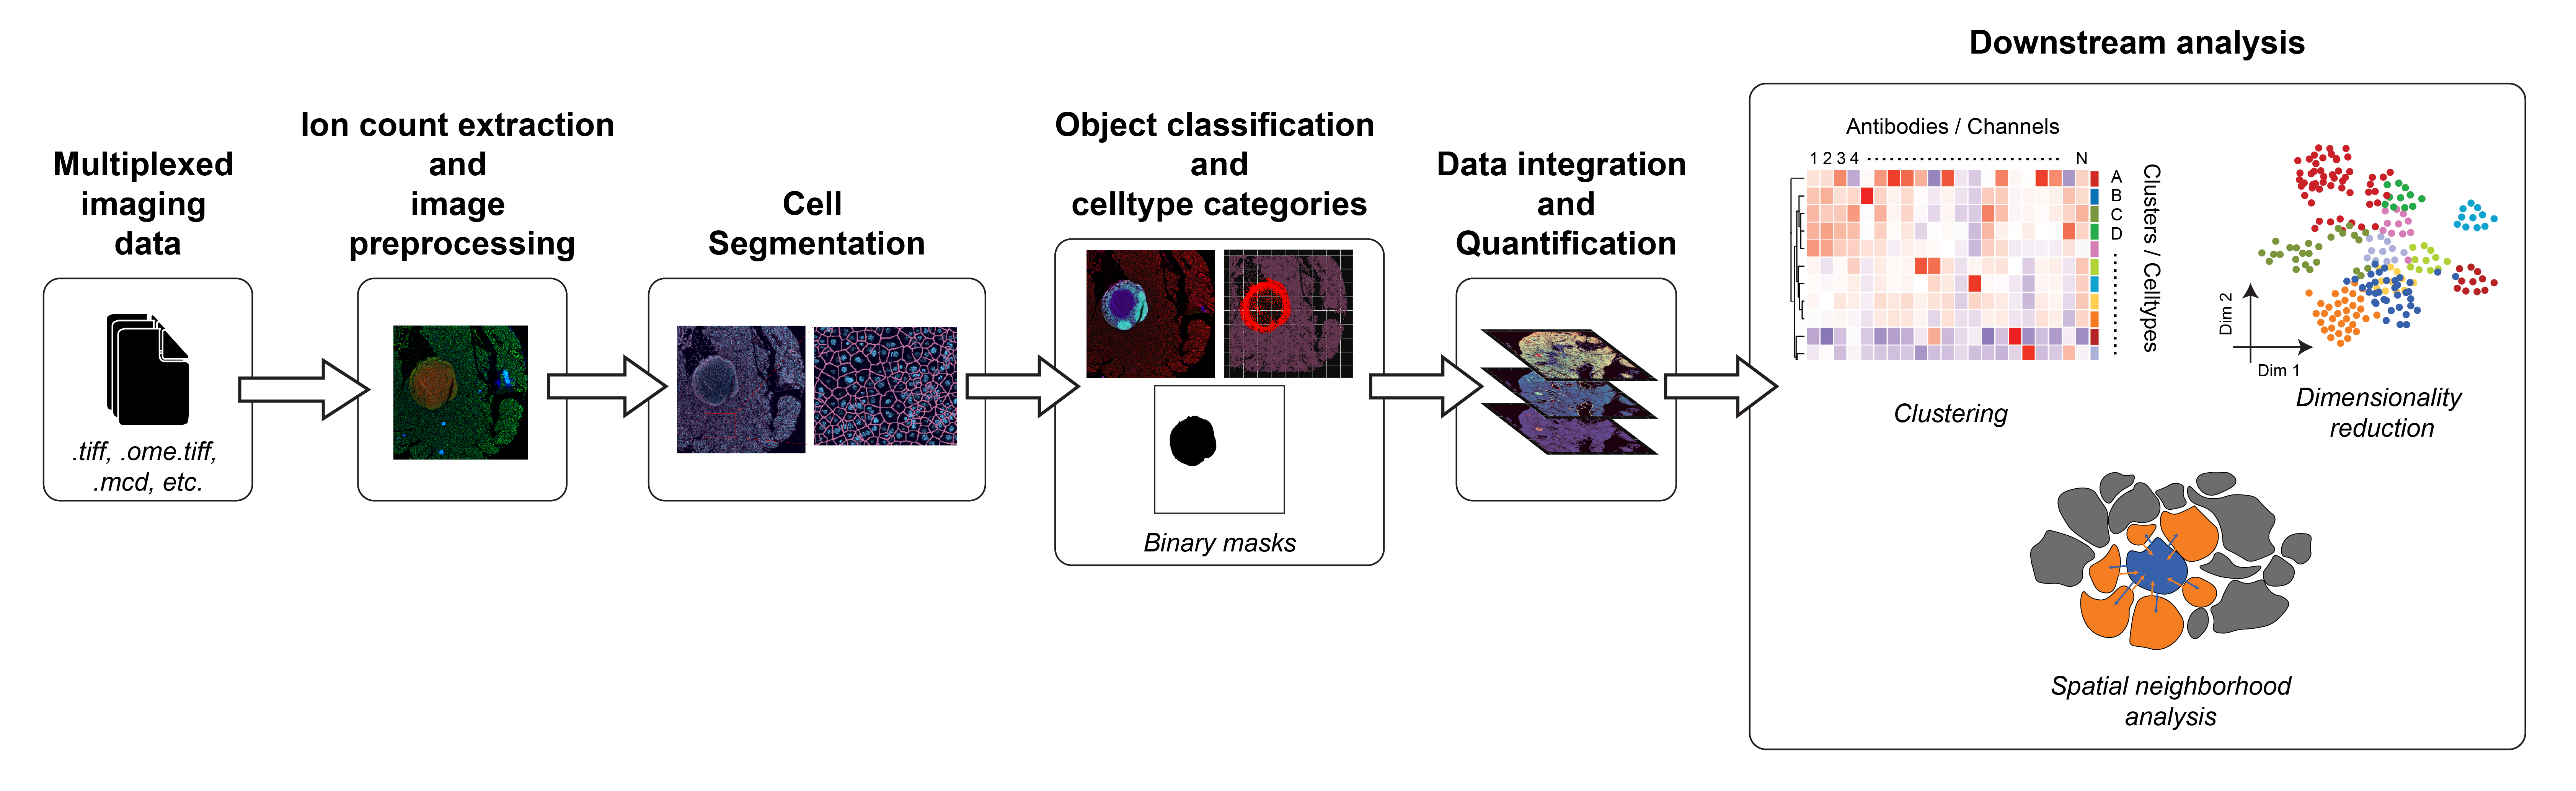
\includegraphics[width=\linewidth]{Chapter1/Fig/F1-14-01.png}
    \caption[Overview of Imaging Mass Cytometry data analysis workflow]{\textbf{Pipeline for processing of multiplexed imaging data from \gls{imc}.} Raw image data extracted from \gls{imc} acquisitions can be used to assess data quality and exploratory visualization. Following pre-processing, the cell-segmentation step involves performing pixel-wise classification into cellular components (nuclei, cytoplasm, cell membrane) or cell-types depending on intended downstream analysis strategies. Segmented images can then used to generate cell binary masks or object binary masks which can be subsequently used to extract cell-level or cell-type information. Several such segmented images and masks can be integrated and quantified to extract the channel intensity across all single-cells. The single-cell data can then be processed with single-cell analysis methods like clustering and \gls{dr}, and additional spatial analysis methods can be employed to obtain a comprehensive understanding of the tissue architecture. \textit{This figure was originally generated by Dr. Matthias Barone and has been adapted here with permission.}}
    \label{fig:chp1_imc_analysis}
\end{figure}


pixel intensity such as hot pixels and speckles \textbf{\cite{milosevic_different_2023}}. Next, cell segmentation represents the most critical step, whereby, certain areas and pixels in the images are defined as objects, cell and cellular compartments. The downstream analyses and the accuracy of the subsequent data and biological interpretation directly depend on the quality and accuracy of this step \textbf{\cite{milosevic_different_2023}}. Therefore, this step must be approached with utmost care, and if necessary, iterations of segmentation should be performed. Advanced techniques using deep convolutional neural networks can help speed up the segmentation process \textbf{\cite{jung_automatic_2019,fujita_cell_2021}}. %The resulting single-cell data can be analyzed with same analysis pipelines used to analyze CyTOF data, with the added dimensions of cell shape, size and, localization. 
Finally, the single-cell, segmented, preprocessed \gls{imc} data can be analyzed with same analysis pipelines used to analyze \gls{cytof} data \textbf{\cite{veenstra_research_2021}}, such as \gls{dr} to simplify data visualization, clustering to identify distinct cellular populations and spatial analysis to examine the distribution and relationship among cell-types. Further, integration with other \textit{-omics} data enrich the biological insights obtained, thereby enabling a comprehensive understanding of tissue architecture and cellular interactions \textbf{(Fig. \ref{fig:chp1_imc_analysis})} \textbf{\cite{veenstra_research_2021}}. \gls{imc} can align with \gls{scr} by providing a detailed spatial context to the molecular profiles obtained from \textit{-omics} analyses. \gls{imc} can map the location of specific cell-types and states identified by \gls{scr} within tissue sections, validate findings from \gls{scr} studies and generate hypotheses about the role of cellular microenvironments in regulating gene expression patterns.\\

\par \gls{imc} has found applications in various research areas including the study of structure and function of normal tissues \textbf{\cite{chang_imaging_2017}} in immunology \textbf{\cite{zhao_spatiotemporal_2018,li_memory_2019}}, the study of the tumor microenvironment \textbf{\cite{jackson_single-cell_2020,moldoveanu_spatially_2022}}, in \gls{t1d} research \textbf{\cite{damond_map_2019,wang_multiplexed_2019}} and in Covid-19 \textbf{\cite{wang_imaging_2020}}. 

% % ***************************************************************
% %************************ %seventh Section %****************************************************************
% \section{Thesis Outline}  %Section - 1.t
% \label{sec:outline}

% The overarching topic of this thesis is the pathogenesis of Type-2 diabetes. 

% investigation of pancreatic islet inflammation and $\beta$-cell dysfunction, on a single-cell level, in the context of \gls{t2d} pathogenesis, using mouse models.  microenvironment in response to 

%\newpage\null\thispagestyle{empty}\newpage